\documentclass[twoside]{book}

% Packages required by doxygen
\usepackage{fixltx2e}
\usepackage{calc}
\usepackage{doxygen}
\usepackage[export]{adjustbox} % also loads graphicx
\usepackage{graphicx}
\usepackage[utf8]{inputenc}
\usepackage{makeidx}
\usepackage{multicol}
\usepackage{multirow}
\PassOptionsToPackage{warn}{textcomp}
\usepackage{textcomp}
\usepackage[nointegrals]{wasysym}
\usepackage[table]{xcolor}

% Font selection
\usepackage[T1]{fontenc}
\usepackage[scaled=.90]{helvet}
\usepackage{courier}
\usepackage{amssymb}
\usepackage{sectsty}
\renewcommand{\familydefault}{\sfdefault}
\allsectionsfont{%
  \fontseries{bc}\selectfont%
  \color{darkgray}%
}
\renewcommand{\DoxyLabelFont}{%
  \fontseries{bc}\selectfont%
  \color{darkgray}%
}
\newcommand{\+}{\discretionary{\mbox{\scriptsize$\hookleftarrow$}}{}{}}

% Page & text layout
\usepackage{geometry}
\geometry{%
  a4paper,%
  top=2.5cm,%
  bottom=2.5cm,%
  left=2.5cm,%
  right=2.5cm%
}
\tolerance=750
\hfuzz=15pt
\hbadness=750
\setlength{\emergencystretch}{15pt}
\setlength{\parindent}{0cm}
\setlength{\parskip}{3ex plus 2ex minus 2ex}
\makeatletter
\renewcommand{\paragraph}{%
  \@startsection{paragraph}{4}{0ex}{-1.0ex}{1.0ex}{%
    \normalfont\normalsize\bfseries\SS@parafont%
  }%
}
\renewcommand{\subparagraph}{%
  \@startsection{subparagraph}{5}{0ex}{-1.0ex}{1.0ex}{%
    \normalfont\normalsize\bfseries\SS@subparafont%
  }%
}
\makeatother

% Headers & footers
\usepackage{fancyhdr}
\pagestyle{fancyplain}
\fancyhead[LE]{\fancyplain{}{\bfseries\thepage}}
\fancyhead[CE]{\fancyplain{}{}}
\fancyhead[RE]{\fancyplain{}{\bfseries\leftmark}}
\fancyhead[LO]{\fancyplain{}{\bfseries\rightmark}}
\fancyhead[CO]{\fancyplain{}{}}
\fancyhead[RO]{\fancyplain{}{\bfseries\thepage}}
\fancyfoot[LE]{\fancyplain{}{}}
\fancyfoot[CE]{\fancyplain{}{}}
\fancyfoot[RE]{\fancyplain{}{\bfseries\scriptsize Generated by Doxygen }}
\fancyfoot[LO]{\fancyplain{}{\bfseries\scriptsize Generated by Doxygen }}
\fancyfoot[CO]{\fancyplain{}{}}
\fancyfoot[RO]{\fancyplain{}{}}
\renewcommand{\footrulewidth}{0.4pt}
\renewcommand{\chaptermark}[1]{%
  \markboth{#1}{}%
}
\renewcommand{\sectionmark}[1]{%
  \markright{\thesection\ #1}%
}

% Indices & bibliography
\usepackage{natbib}
\usepackage[titles]{tocloft}
\setcounter{tocdepth}{3}
\setcounter{secnumdepth}{5}
\makeindex

% Hyperlinks (required, but should be loaded last)
\usepackage{ifpdf}
\ifpdf
  \usepackage[pdftex,pagebackref=true]{hyperref}
\else
  \usepackage[ps2pdf,pagebackref=true]{hyperref}
\fi
\hypersetup{%
  colorlinks=true,%
  linkcolor=blue,%
  citecolor=blue,%
  unicode%
}

% Custom commands
\newcommand{\clearemptydoublepage}{%
  \newpage{\pagestyle{empty}\cleardoublepage}%
}

\usepackage{caption}
\captionsetup{labelsep=space,justification=centering,font={bf},singlelinecheck=off,skip=4pt,position=top}

%===== C O N T E N T S =====

\begin{document}

% Titlepage & ToC
\hypersetup{pageanchor=false,
             bookmarksnumbered=true,
             pdfencoding=unicode
            }
\pagenumbering{alph}
\begin{titlepage}
\vspace*{7cm}
\begin{center}%
{\Large Projeto A\+E\+DA \\[1ex]\large 2 }\\
\vspace*{1cm}
{\large Generated by Doxygen 1.8.12}\\
\end{center}
\end{titlepage}
\clearemptydoublepage
\pagenumbering{roman}
\tableofcontents
\clearemptydoublepage
\pagenumbering{arabic}
\hypersetup{pageanchor=true}

%--- Begin generated contents ---
\chapter{Hierarchical Index}
\section{Class Hierarchy}
This inheritance list is sorted roughly, but not completely, alphabetically\+:\begin{DoxyCompactList}
\item \contentsline{section}{Binary\+Node$<$ Comparable $>$}{\pageref{class_binary_node}}{}
\item \contentsline{section}{Binary\+Node$<$ Player\+\_\+node $>$}{\pageref{class_binary_node}}{}
\item \contentsline{section}{B\+ST$<$ Comparable $>$}{\pageref{class_b_s_t}}{}
\item \contentsline{section}{B\+ST$<$ Player\+\_\+node $>$}{\pageref{class_b_s_t}}{}
\item \contentsline{section}{B\+S\+T\+Itr\+In$<$ Comparable $>$}{\pageref{class_b_s_t_itr_in}}{}
\item \contentsline{section}{B\+S\+T\+Itr\+Level$<$ Comparable $>$}{\pageref{class_b_s_t_itr_level}}{}
\item \contentsline{section}{B\+S\+T\+Itr\+Post$<$ Comparable $>$}{\pageref{class_b_s_t_itr_post}}{}
\item \contentsline{section}{B\+S\+T\+Itr\+Pre$<$ Comparable $>$}{\pageref{class_b_s_t_itr_pre}}{}
\item \contentsline{section}{Club}{\pageref{class_club}}{}
\item \contentsline{section}{Date}{\pageref{class_date}}{}
\item \contentsline{section}{Duplicate\+Name}{\pageref{class_duplicate_name}}{}
\item \contentsline{section}{Event}{\pageref{class_event}}{}
\begin{DoxyCompactList}
\item \contentsline{section}{Tournament}{\pageref{class_tournament}}{}
\item \contentsline{section}{Training}{\pageref{class_training}}{}
\end{DoxyCompactList}
\item \contentsline{section}{hash\+Funcs}{\pageref{structhash_funcs}}{}
\item \contentsline{section}{Invalid\+Date}{\pageref{class_invalid_date}}{}
\item \contentsline{section}{Invalid\+Player}{\pageref{class_invalid_player}}{}
\item \contentsline{section}{Level}{\pageref{class_level}}{}
\begin{DoxyCompactList}
\item \contentsline{section}{Juniors}{\pageref{class_juniors}}{}
\item \contentsline{section}{Juveniles}{\pageref{class_juveniles}}{}
\item \contentsline{section}{Minis}{\pageref{class_minis}}{}
\item \contentsline{section}{Seniors}{\pageref{class_seniors}}{}
\end{DoxyCompactList}
\item \contentsline{section}{Player}{\pageref{class_player}}{}
\item \contentsline{section}{Player\+\_\+node}{\pageref{struct_player__node}}{}
\item \contentsline{section}{Player\+\_\+queue}{\pageref{struct_player__queue}}{}
\end{DoxyCompactList}

\chapter{Class Index}
\section{Class List}
Here are the classes, structs, unions and interfaces with brief descriptions\+:\begin{DoxyCompactList}
\item\contentsline{section}{\hyperlink{class_binary_node}{Binary\+Node$<$ Comparable $>$} }{\pageref{class_binary_node}}{}
\item\contentsline{section}{\hyperlink{class_b_s_t}{B\+S\+T$<$ Comparable $>$} }{\pageref{class_b_s_t}}{}
\item\contentsline{section}{\hyperlink{class_b_s_t_itr_in}{B\+S\+T\+Itr\+In$<$ Comparable $>$} }{\pageref{class_b_s_t_itr_in}}{}
\item\contentsline{section}{\hyperlink{class_b_s_t_itr_level}{B\+S\+T\+Itr\+Level$<$ Comparable $>$} }{\pageref{class_b_s_t_itr_level}}{}
\item\contentsline{section}{\hyperlink{class_b_s_t_itr_post}{B\+S\+T\+Itr\+Post$<$ Comparable $>$} }{\pageref{class_b_s_t_itr_post}}{}
\item\contentsline{section}{\hyperlink{class_b_s_t_itr_pre}{B\+S\+T\+Itr\+Pre$<$ Comparable $>$} }{\pageref{class_b_s_t_itr_pre}}{}
\item\contentsline{section}{\hyperlink{class_club}{Club} \\*Holds all the information about the \hyperlink{class_club}{Club} }{\pageref{class_club}}{}
\item\contentsline{section}{\hyperlink{class_date}{Date} \\*Class that represents a \hyperlink{class_date}{Date} of the calendar }{\pageref{class_date}}{}
\item\contentsline{section}{\hyperlink{class_duplicate_name}{Duplicate\+Name} \\*Represents an Invalid Players }{\pageref{class_duplicate_name}}{}
\item\contentsline{section}{\hyperlink{class_event}{Event} \\*Class to hold information about an event }{\pageref{class_event}}{}
\item\contentsline{section}{\hyperlink{structhash_funcs}{hash\+Funcs} \\*Functions used in \hyperlink{class_club}{Club} member variable future\+\_\+birthdays Chained Hash-\/\+Table }{\pageref{structhash_funcs}}{}
\item\contentsline{section}{\hyperlink{class_invalid_date}{Invalid\+Date} \\*Represents an Invalid \hyperlink{class_date}{Date} }{\pageref{class_invalid_date}}{}
\item\contentsline{section}{\hyperlink{class_invalid_player}{Invalid\+Player} \\*Represents an Invalid Players }{\pageref{class_invalid_player}}{}
\item\contentsline{section}{\hyperlink{class_juniors}{Juniors} \\*Holds all the information about the \hyperlink{class_level}{Level} \hyperlink{class_juniors}{Juniors} }{\pageref{class_juniors}}{}
\item\contentsline{section}{\hyperlink{class_juveniles}{Juveniles} \\*Holds all the information about the \hyperlink{class_level}{Level} \hyperlink{class_juveniles}{Juveniles} }{\pageref{class_juveniles}}{}
\item\contentsline{section}{\hyperlink{class_level}{Level} \\*Holds all the information about the \hyperlink{class_club}{Club} }{\pageref{class_level}}{}
\item\contentsline{section}{\hyperlink{class_minis}{Minis} \\*Holds all the information about the \hyperlink{class_level}{Level} \hyperlink{class_minis}{Minis} }{\pageref{class_minis}}{}
\item\contentsline{section}{\hyperlink{class_player}{Player} \\*Holds all the information about a given \hyperlink{class_player}{Player} }{\pageref{class_player}}{}
\item\contentsline{section}{\hyperlink{struct_player__node}{Player\+\_\+node} \\*Struct to store the \hyperlink{class_player}{Player} in a \hyperlink{class_b_s_t}{B\+ST} }{\pageref{struct_player__node}}{}
\item\contentsline{section}{\hyperlink{struct_player__queue}{Player\+\_\+queue} \\*Struct to store the \hyperlink{class_player}{Player} in a priority queue }{\pageref{struct_player__queue}}{}
\item\contentsline{section}{\hyperlink{class_seniors}{Seniors} \\*Holds all the information about the \hyperlink{class_level}{Level} \hyperlink{class_seniors}{Seniors} }{\pageref{class_seniors}}{}
\item\contentsline{section}{\hyperlink{class_tournament}{Tournament} \\*Used to host information about a single \hyperlink{class_tournament}{Tournament} }{\pageref{class_tournament}}{}
\item\contentsline{section}{\hyperlink{class_training}{Training} \\*Used to host information about a single \hyperlink{class_training}{Training} }{\pageref{class_training}}{}
\end{DoxyCompactList}

\chapter{File Index}
\section{File List}
Here is a list of all files with brief descriptions\+:\begin{DoxyCompactList}
\item\contentsline{section}{/home/oco/\+Documents/\+Cprojects/\+Athletes/projecto -\/ V2/\+Headers/\hyperlink{_b_s_t_8h}{B\+S\+T.\+h} }{\pageref{_b_s_t_8h}}{}
\item\contentsline{section}{/home/oco/\+Documents/\+Cprojects/\+Athletes/projecto -\/ V2/\+Headers/\hyperlink{_club_8h}{Club.\+h} }{\pageref{_club_8h}}{}
\item\contentsline{section}{/home/oco/\+Documents/\+Cprojects/\+Athletes/projecto -\/ V2/\+Headers/\hyperlink{_date_8h}{Date.\+h} }{\pageref{_date_8h}}{}
\item\contentsline{section}{/home/oco/\+Documents/\+Cprojects/\+Athletes/projecto -\/ V2/\+Headers/\hyperlink{_event_8h}{Event.\+h} }{\pageref{_event_8h}}{}
\item\contentsline{section}{/home/oco/\+Documents/\+Cprojects/\+Athletes/projecto -\/ V2/\+Headers/\hyperlink{exceptions_8h}{exceptions.\+h} }{\pageref{exceptions_8h}}{}
\item\contentsline{section}{/home/oco/\+Documents/\+Cprojects/\+Athletes/projecto -\/ V2/\+Headers/\hyperlink{_juniors_8h}{Juniors.\+h} }{\pageref{_juniors_8h}}{}
\item\contentsline{section}{/home/oco/\+Documents/\+Cprojects/\+Athletes/projecto -\/ V2/\+Headers/\hyperlink{_juveniles_8h}{Juveniles.\+h} }{\pageref{_juveniles_8h}}{}
\item\contentsline{section}{/home/oco/\+Documents/\+Cprojects/\+Athletes/projecto -\/ V2/\+Headers/\hyperlink{_level_8h}{Level.\+h} }{\pageref{_level_8h}}{}
\item\contentsline{section}{/home/oco/\+Documents/\+Cprojects/\+Athletes/projecto -\/ V2/\+Headers/\hyperlink{menus_8h}{menus.\+h} }{\pageref{menus_8h}}{}
\item\contentsline{section}{/home/oco/\+Documents/\+Cprojects/\+Athletes/projecto -\/ V2/\+Headers/\hyperlink{_minis_8h}{Minis.\+h} }{\pageref{_minis_8h}}{}
\item\contentsline{section}{/home/oco/\+Documents/\+Cprojects/\+Athletes/projecto -\/ V2/\+Headers/\hyperlink{_player_8h}{Player.\+h} }{\pageref{_player_8h}}{}
\item\contentsline{section}{/home/oco/\+Documents/\+Cprojects/\+Athletes/projecto -\/ V2/\+Headers/\hyperlink{_seniors_8h}{Seniors.\+h} }{\pageref{_seniors_8h}}{}
\item\contentsline{section}{/home/oco/\+Documents/\+Cprojects/\+Athletes/projecto -\/ V2/\+Headers/\hyperlink{_tournament_8h}{Tournament.\+h} }{\pageref{_tournament_8h}}{}
\item\contentsline{section}{/home/oco/\+Documents/\+Cprojects/\+Athletes/projecto -\/ V2/\+Headers/\hyperlink{_training_8h}{Training.\+h} }{\pageref{_training_8h}}{}
\item\contentsline{section}{/home/oco/\+Documents/\+Cprojects/\+Athletes/projecto -\/ V2/\+Headers/\hyperlink{utilities_8h}{utilities.\+h} }{\pageref{utilities_8h}}{}
\item\contentsline{section}{/home/oco/\+Documents/\+Cprojects/\+Athletes/projecto -\/ V2/\+Source/\hyperlink{_club_8cpp}{Club.\+cpp} }{\pageref{_club_8cpp}}{}
\item\contentsline{section}{/home/oco/\+Documents/\+Cprojects/\+Athletes/projecto -\/ V2/\+Source/\hyperlink{_date_8cpp}{Date.\+cpp} }{\pageref{_date_8cpp}}{}
\item\contentsline{section}{/home/oco/\+Documents/\+Cprojects/\+Athletes/projecto -\/ V2/\+Source/\hyperlink{exceptions_8cpp}{exceptions.\+cpp} }{\pageref{exceptions_8cpp}}{}
\item\contentsline{section}{/home/oco/\+Documents/\+Cprojects/\+Athletes/projecto -\/ V2/\+Source/\hyperlink{_juniors_8cpp}{Juniors.\+cpp} }{\pageref{_juniors_8cpp}}{}
\item\contentsline{section}{/home/oco/\+Documents/\+Cprojects/\+Athletes/projecto -\/ V2/\+Source/\hyperlink{_juveniles_8cpp}{Juveniles.\+cpp} }{\pageref{_juveniles_8cpp}}{}
\item\contentsline{section}{/home/oco/\+Documents/\+Cprojects/\+Athletes/projecto -\/ V2/\+Source/\hyperlink{_level_8cpp}{Level.\+cpp} }{\pageref{_level_8cpp}}{}
\item\contentsline{section}{/home/oco/\+Documents/\+Cprojects/\+Athletes/projecto -\/ V2/\+Source/\hyperlink{main_8cpp}{main.\+cpp} }{\pageref{main_8cpp}}{}
\item\contentsline{section}{/home/oco/\+Documents/\+Cprojects/\+Athletes/projecto -\/ V2/\+Source/\hyperlink{menus_8cpp}{menus.\+cpp} }{\pageref{menus_8cpp}}{}
\item\contentsline{section}{/home/oco/\+Documents/\+Cprojects/\+Athletes/projecto -\/ V2/\+Source/\hyperlink{_minis_8cpp}{Minis.\+cpp} }{\pageref{_minis_8cpp}}{}
\item\contentsline{section}{/home/oco/\+Documents/\+Cprojects/\+Athletes/projecto -\/ V2/\+Source/\hyperlink{_player_8cpp}{Player.\+cpp} }{\pageref{_player_8cpp}}{}
\item\contentsline{section}{/home/oco/\+Documents/\+Cprojects/\+Athletes/projecto -\/ V2/\+Source/\hyperlink{_seniors_8cpp}{Seniors.\+cpp} }{\pageref{_seniors_8cpp}}{}
\item\contentsline{section}{/home/oco/\+Documents/\+Cprojects/\+Athletes/projecto -\/ V2/\+Source/\hyperlink{_tournament_8cpp}{Tournament.\+cpp} }{\pageref{_tournament_8cpp}}{}
\item\contentsline{section}{/home/oco/\+Documents/\+Cprojects/\+Athletes/projecto -\/ V2/\+Source/\hyperlink{_training_8cpp}{Training.\+cpp} }{\pageref{_training_8cpp}}{}
\item\contentsline{section}{/home/oco/\+Documents/\+Cprojects/\+Athletes/projecto -\/ V2/\+Source/\hyperlink{utilities_8cpp}{utilities.\+cpp} }{\pageref{utilities_8cpp}}{}
\end{DoxyCompactList}

\chapter{Class Documentation}
\hypertarget{class_binary_node}{}\section{Binary\+Node$<$ Comparable $>$ Class Template Reference}
\label{class_binary_node}\index{Binary\+Node$<$ Comparable $>$@{Binary\+Node$<$ Comparable $>$}}


{\ttfamily \#include $<$B\+S\+T.\+h$>$}

\subsection*{Friends}
\begin{DoxyCompactItemize}
\item 
class \hyperlink{class_binary_node_a28a1adb9906f3ff7e12c2cb6fa2bd54e}{B\+S\+T$<$ Comparable $>$}
\item 
class \hyperlink{class_binary_node_aab3993acac2ab24a0b59edb0c3acc775}{B\+S\+T\+Itr\+In$<$ Comparable $>$}
\item 
class \hyperlink{class_binary_node_a45a55df6f11541416d4ea7684c575c1a}{B\+S\+T\+Itr\+Pre$<$ Comparable $>$}
\item 
class \hyperlink{class_binary_node_a5dc153694be266f6e772659486219da7}{B\+S\+T\+Itr\+Post$<$ Comparable $>$}
\item 
class \hyperlink{class_binary_node_a26ff00bc0d87069aed877f10fd3c80a8}{B\+S\+T\+Itr\+Level$<$ Comparable $>$}
\end{DoxyCompactItemize}


\subsection{Detailed Description}
\subsubsection*{template$<$class Comparable$>$\newline
class Binary\+Node$<$ Comparable $>$}



Definition at line 38 of file B\+S\+T.\+h.



\subsection{Friends And Related Function Documentation}
\hypertarget{class_binary_node_a28a1adb9906f3ff7e12c2cb6fa2bd54e}{}\label{class_binary_node_a28a1adb9906f3ff7e12c2cb6fa2bd54e} 
\index{Binary\+Node@{Binary\+Node}!B\+S\+T$<$ Comparable $>$@{B\+S\+T$<$ Comparable $>$}}
\index{B\+S\+T$<$ Comparable $>$@{B\+S\+T$<$ Comparable $>$}!Binary\+Node@{Binary\+Node}}
\subsubsection{\texorpdfstring{B\+S\+T$<$ Comparable $>$}{BST< Comparable >}}
{\footnotesize\ttfamily template$<$class Comparable$>$ \\
friend class \hyperlink{class_b_s_t}{B\+ST}$<$ Comparable $>$\hspace{0.3cm}{\ttfamily [friend]}}



Definition at line 47 of file B\+S\+T.\+h.

\hypertarget{class_binary_node_aab3993acac2ab24a0b59edb0c3acc775}{}\label{class_binary_node_aab3993acac2ab24a0b59edb0c3acc775} 
\index{Binary\+Node@{Binary\+Node}!B\+S\+T\+Itr\+In$<$ Comparable $>$@{B\+S\+T\+Itr\+In$<$ Comparable $>$}}
\index{B\+S\+T\+Itr\+In$<$ Comparable $>$@{B\+S\+T\+Itr\+In$<$ Comparable $>$}!Binary\+Node@{Binary\+Node}}
\subsubsection{\texorpdfstring{B\+S\+T\+Itr\+In$<$ Comparable $>$}{BSTItrIn< Comparable >}}
{\footnotesize\ttfamily template$<$class Comparable$>$ \\
friend class \hyperlink{class_b_s_t_itr_in}{B\+S\+T\+Itr\+In}$<$ Comparable $>$\hspace{0.3cm}{\ttfamily [friend]}}



Definition at line 48 of file B\+S\+T.\+h.

\hypertarget{class_binary_node_a26ff00bc0d87069aed877f10fd3c80a8}{}\label{class_binary_node_a26ff00bc0d87069aed877f10fd3c80a8} 
\index{Binary\+Node@{Binary\+Node}!B\+S\+T\+Itr\+Level$<$ Comparable $>$@{B\+S\+T\+Itr\+Level$<$ Comparable $>$}}
\index{B\+S\+T\+Itr\+Level$<$ Comparable $>$@{B\+S\+T\+Itr\+Level$<$ Comparable $>$}!Binary\+Node@{Binary\+Node}}
\subsubsection{\texorpdfstring{B\+S\+T\+Itr\+Level$<$ Comparable $>$}{BSTItrLevel< Comparable >}}
{\footnotesize\ttfamily template$<$class Comparable$>$ \\
friend class \hyperlink{class_b_s_t_itr_level}{B\+S\+T\+Itr\+Level}$<$ Comparable $>$\hspace{0.3cm}{\ttfamily [friend]}}



Definition at line 51 of file B\+S\+T.\+h.

\hypertarget{class_binary_node_a5dc153694be266f6e772659486219da7}{}\label{class_binary_node_a5dc153694be266f6e772659486219da7} 
\index{Binary\+Node@{Binary\+Node}!B\+S\+T\+Itr\+Post$<$ Comparable $>$@{B\+S\+T\+Itr\+Post$<$ Comparable $>$}}
\index{B\+S\+T\+Itr\+Post$<$ Comparable $>$@{B\+S\+T\+Itr\+Post$<$ Comparable $>$}!Binary\+Node@{Binary\+Node}}
\subsubsection{\texorpdfstring{B\+S\+T\+Itr\+Post$<$ Comparable $>$}{BSTItrPost< Comparable >}}
{\footnotesize\ttfamily template$<$class Comparable$>$ \\
friend class \hyperlink{class_b_s_t_itr_post}{B\+S\+T\+Itr\+Post}$<$ Comparable $>$\hspace{0.3cm}{\ttfamily [friend]}}



Definition at line 50 of file B\+S\+T.\+h.

\hypertarget{class_binary_node_a45a55df6f11541416d4ea7684c575c1a}{}\label{class_binary_node_a45a55df6f11541416d4ea7684c575c1a} 
\index{Binary\+Node@{Binary\+Node}!B\+S\+T\+Itr\+Pre$<$ Comparable $>$@{B\+S\+T\+Itr\+Pre$<$ Comparable $>$}}
\index{B\+S\+T\+Itr\+Pre$<$ Comparable $>$@{B\+S\+T\+Itr\+Pre$<$ Comparable $>$}!Binary\+Node@{Binary\+Node}}
\subsubsection{\texorpdfstring{B\+S\+T\+Itr\+Pre$<$ Comparable $>$}{BSTItrPre< Comparable >}}
{\footnotesize\ttfamily template$<$class Comparable$>$ \\
friend class \hyperlink{class_b_s_t_itr_pre}{B\+S\+T\+Itr\+Pre}$<$ Comparable $>$\hspace{0.3cm}{\ttfamily [friend]}}



Definition at line 49 of file B\+S\+T.\+h.



The documentation for this class was generated from the following file\+:\begin{DoxyCompactItemize}
\item 
/home/oco/\+Documents/\+Cprojects/\+Athletes/projecto -\/ V2/\+Headers/\hyperlink{_b_s_t_8h}{B\+S\+T.\+h}\end{DoxyCompactItemize}

\hypertarget{class_b_s_t}{}\section{B\+ST$<$ Comparable $>$ Class Template Reference}
\label{class_b_s_t}\index{B\+S\+T$<$ Comparable $>$@{B\+S\+T$<$ Comparable $>$}}


{\ttfamily \#include $<$B\+S\+T.\+h$>$}

\subsection*{Public Member Functions}
\begin{DoxyCompactItemize}
\item 
\hyperlink{class_b_s_t_a3185a79cf472271f122a97d0f59022d1}{B\+ST} (const Comparable \&not\+Found)
\item 
\hyperlink{class_b_s_t_a163232cc6ffcbd1a51707efcc3fa36ca}{B\+ST} (const \hyperlink{class_b_s_t}{B\+ST} \&rhs)
\item 
\hyperlink{class_b_s_t_abf3125f968641c8726101c5dd18f36be}{$\sim$\+B\+ST} ()
\item 
const Comparable \& \hyperlink{class_b_s_t_aa52491ff35aec517961937a17a9fa493}{find\+Min} () const
\item 
const Comparable \& \hyperlink{class_b_s_t_a03485f3b0b150f1e69a12c28d26d8092}{find\+Max} () const
\item 
const Comparable \& \hyperlink{class_b_s_t_aaf4eb6869f68db0069534f7b2dfbe53b}{find} (const Comparable \&x) const
\item 
bool \hyperlink{class_b_s_t_a10fd737b2be62437023407fdc123f728}{is\+Empty} () const
\item 
void \hyperlink{class_b_s_t_a91e830925c48040d4c4dbb7d971c3bfe}{print\+Tree} () const
\item 
void \hyperlink{class_b_s_t_a050d829503a88714c4ad0773cf6d3af6}{make\+Empty} ()
\item 
void \hyperlink{class_b_s_t_a2b117df6521c7d61dac75ff2c938bae7}{insert} (const Comparable \&x)
\item 
void \hyperlink{class_b_s_t_a6f01a0b44daf82a42022b6eb4c0df7a2}{remove} (const Comparable \&x)
\item 
const \hyperlink{class_b_s_t}{B\+ST} \& \hyperlink{class_b_s_t_aa80c39f454c89d4a202be3d1445823f3}{operator=} (const \hyperlink{class_b_s_t}{B\+ST} \&rhs)
\end{DoxyCompactItemize}
\subsection*{Friends}
\begin{DoxyCompactItemize}
\item 
class \hyperlink{class_b_s_t_aab3993acac2ab24a0b59edb0c3acc775}{B\+S\+T\+Itr\+In$<$ Comparable $>$}
\item 
class \hyperlink{class_b_s_t_a45a55df6f11541416d4ea7684c575c1a}{B\+S\+T\+Itr\+Pre$<$ Comparable $>$}
\item 
class \hyperlink{class_b_s_t_a5dc153694be266f6e772659486219da7}{B\+S\+T\+Itr\+Post$<$ Comparable $>$}
\item 
class \hyperlink{class_b_s_t_a26ff00bc0d87069aed877f10fd3c80a8}{B\+S\+T\+Itr\+Level$<$ Comparable $>$}
\end{DoxyCompactItemize}


\subsection{Detailed Description}
\subsubsection*{template$<$class Comparable$>$\newline
class B\+S\+T$<$ Comparable $>$}



Definition at line 35 of file B\+S\+T.\+h.



\subsection{Constructor \& Destructor Documentation}
\hypertarget{class_b_s_t_a3185a79cf472271f122a97d0f59022d1}{}\label{class_b_s_t_a3185a79cf472271f122a97d0f59022d1} 
\index{B\+ST@{B\+ST}!B\+ST@{B\+ST}}
\index{B\+ST@{B\+ST}!B\+ST@{B\+ST}}
\subsubsection{\texorpdfstring{B\+S\+T()}{BST()}\hspace{0.1cm}{\footnotesize\ttfamily [1/2]}}
{\footnotesize\ttfamily template$<$class Comparable$>$ \\
\hyperlink{class_b_s_t}{B\+ST}$<$ Comparable $>$\+::\hyperlink{class_b_s_t}{B\+ST} (\begin{DoxyParamCaption}\item[{const Comparable \&}]{not\+Found }\end{DoxyParamCaption})\hspace{0.3cm}{\ttfamily [explicit]}}



Definition at line 98 of file B\+S\+T.\+h.

\hypertarget{class_b_s_t_a163232cc6ffcbd1a51707efcc3fa36ca}{}\label{class_b_s_t_a163232cc6ffcbd1a51707efcc3fa36ca} 
\index{B\+ST@{B\+ST}!B\+ST@{B\+ST}}
\index{B\+ST@{B\+ST}!B\+ST@{B\+ST}}
\subsubsection{\texorpdfstring{B\+S\+T()}{BST()}\hspace{0.1cm}{\footnotesize\ttfamily [2/2]}}
{\footnotesize\ttfamily template$<$class Comparable$>$ \\
\hyperlink{class_b_s_t}{B\+ST}$<$ Comparable $>$\+::\hyperlink{class_b_s_t}{B\+ST} (\begin{DoxyParamCaption}\item[{const \hyperlink{class_b_s_t}{B\+ST}$<$ Comparable $>$ \&}]{rhs }\end{DoxyParamCaption})}



Definition at line 103 of file B\+S\+T.\+h.

\hypertarget{class_b_s_t_abf3125f968641c8726101c5dd18f36be}{}\label{class_b_s_t_abf3125f968641c8726101c5dd18f36be} 
\index{B\+ST@{B\+ST}!````~B\+ST@{$\sim$\+B\+ST}}
\index{````~B\+ST@{$\sim$\+B\+ST}!B\+ST@{B\+ST}}
\subsubsection{\texorpdfstring{$\sim$\+B\+S\+T()}{~BST()}}
{\footnotesize\ttfamily template$<$class Comparable $>$ \\
\hyperlink{class_b_s_t}{B\+ST}$<$ Comparable $>$\+::$\sim$\hyperlink{class_b_s_t}{B\+ST} (\begin{DoxyParamCaption}{ }\end{DoxyParamCaption})}



Definition at line 110 of file B\+S\+T.\+h.



\subsection{Member Function Documentation}
\hypertarget{class_b_s_t_aaf4eb6869f68db0069534f7b2dfbe53b}{}\label{class_b_s_t_aaf4eb6869f68db0069534f7b2dfbe53b} 
\index{B\+ST@{B\+ST}!find@{find}}
\index{find@{find}!B\+ST@{B\+ST}}
\subsubsection{\texorpdfstring{find()}{find()}}
{\footnotesize\ttfamily template$<$class Comparable$>$ \\
const Comparable \& \hyperlink{class_b_s_t}{B\+ST}$<$ Comparable $>$\+::find (\begin{DoxyParamCaption}\item[{const Comparable \&}]{x }\end{DoxyParamCaption}) const}



Definition at line 141 of file B\+S\+T.\+h.

\hypertarget{class_b_s_t_a03485f3b0b150f1e69a12c28d26d8092}{}\label{class_b_s_t_a03485f3b0b150f1e69a12c28d26d8092} 
\index{B\+ST@{B\+ST}!find\+Max@{find\+Max}}
\index{find\+Max@{find\+Max}!B\+ST@{B\+ST}}
\subsubsection{\texorpdfstring{find\+Max()}{findMax()}}
{\footnotesize\ttfamily template$<$class Comparable $>$ \\
const Comparable \& \hyperlink{class_b_s_t}{B\+ST}$<$ Comparable $>$\+::find\+Max (\begin{DoxyParamCaption}{ }\end{DoxyParamCaption}) const}



Definition at line 134 of file B\+S\+T.\+h.

\hypertarget{class_b_s_t_aa52491ff35aec517961937a17a9fa493}{}\label{class_b_s_t_aa52491ff35aec517961937a17a9fa493} 
\index{B\+ST@{B\+ST}!find\+Min@{find\+Min}}
\index{find\+Min@{find\+Min}!B\+ST@{B\+ST}}
\subsubsection{\texorpdfstring{find\+Min()}{findMin()}}
{\footnotesize\ttfamily template$<$class Comparable $>$ \\
const Comparable \& \hyperlink{class_b_s_t}{B\+ST}$<$ Comparable $>$\+::find\+Min (\begin{DoxyParamCaption}{ }\end{DoxyParamCaption}) const}



Definition at line 128 of file B\+S\+T.\+h.

\hypertarget{class_b_s_t_a2b117df6521c7d61dac75ff2c938bae7}{}\label{class_b_s_t_a2b117df6521c7d61dac75ff2c938bae7} 
\index{B\+ST@{B\+ST}!insert@{insert}}
\index{insert@{insert}!B\+ST@{B\+ST}}
\subsubsection{\texorpdfstring{insert()}{insert()}}
{\footnotesize\ttfamily template$<$class Comparable$>$ \\
void \hyperlink{class_b_s_t}{B\+ST}$<$ Comparable $>$\+::insert (\begin{DoxyParamCaption}\item[{const Comparable \&}]{x }\end{DoxyParamCaption})}



Definition at line 116 of file B\+S\+T.\+h.

\hypertarget{class_b_s_t_a10fd737b2be62437023407fdc123f728}{}\label{class_b_s_t_a10fd737b2be62437023407fdc123f728} 
\index{B\+ST@{B\+ST}!is\+Empty@{is\+Empty}}
\index{is\+Empty@{is\+Empty}!B\+ST@{B\+ST}}
\subsubsection{\texorpdfstring{is\+Empty()}{isEmpty()}}
{\footnotesize\ttfamily template$<$class Comparable $>$ \\
bool \hyperlink{class_b_s_t}{B\+ST}$<$ Comparable $>$\+::is\+Empty (\begin{DoxyParamCaption}{ }\end{DoxyParamCaption}) const}



Definition at line 153 of file B\+S\+T.\+h.

\hypertarget{class_b_s_t_a050d829503a88714c4ad0773cf6d3af6}{}\label{class_b_s_t_a050d829503a88714c4ad0773cf6d3af6} 
\index{B\+ST@{B\+ST}!make\+Empty@{make\+Empty}}
\index{make\+Empty@{make\+Empty}!B\+ST@{B\+ST}}
\subsubsection{\texorpdfstring{make\+Empty()}{makeEmpty()}}
{\footnotesize\ttfamily template$<$class Comparable $>$ \\
void \hyperlink{class_b_s_t}{B\+ST}$<$ Comparable $>$\+::make\+Empty (\begin{DoxyParamCaption}{ }\end{DoxyParamCaption})}



Definition at line 147 of file B\+S\+T.\+h.

\hypertarget{class_b_s_t_aa80c39f454c89d4a202be3d1445823f3}{}\label{class_b_s_t_aa80c39f454c89d4a202be3d1445823f3} 
\index{B\+ST@{B\+ST}!operator=@{operator=}}
\index{operator=@{operator=}!B\+ST@{B\+ST}}
\subsubsection{\texorpdfstring{operator=()}{operator=()}}
{\footnotesize\ttfamily template$<$class Comparable $>$ \\
const \hyperlink{class_b_s_t}{B\+ST}$<$ Comparable $>$ \& \hyperlink{class_b_s_t}{B\+ST}$<$ Comparable $>$\+::operator= (\begin{DoxyParamCaption}\item[{const \hyperlink{class_b_s_t}{B\+ST}$<$ Comparable $>$ \&}]{rhs }\end{DoxyParamCaption})}



Definition at line 171 of file B\+S\+T.\+h.

\hypertarget{class_b_s_t_a91e830925c48040d4c4dbb7d971c3bfe}{}\label{class_b_s_t_a91e830925c48040d4c4dbb7d971c3bfe} 
\index{B\+ST@{B\+ST}!print\+Tree@{print\+Tree}}
\index{print\+Tree@{print\+Tree}!B\+ST@{B\+ST}}
\subsubsection{\texorpdfstring{print\+Tree()}{printTree()}}
{\footnotesize\ttfamily template$<$class Comparable $>$ \\
void \hyperlink{class_b_s_t}{B\+ST}$<$ Comparable $>$\+::print\+Tree (\begin{DoxyParamCaption}{ }\end{DoxyParamCaption}) const}



Definition at line 160 of file B\+S\+T.\+h.

\hypertarget{class_b_s_t_a6f01a0b44daf82a42022b6eb4c0df7a2}{}\label{class_b_s_t_a6f01a0b44daf82a42022b6eb4c0df7a2} 
\index{B\+ST@{B\+ST}!remove@{remove}}
\index{remove@{remove}!B\+ST@{B\+ST}}
\subsubsection{\texorpdfstring{remove()}{remove()}}
{\footnotesize\ttfamily template$<$class Comparable$>$ \\
void \hyperlink{class_b_s_t}{B\+ST}$<$ Comparable $>$\+::remove (\begin{DoxyParamCaption}\item[{const Comparable \&}]{x }\end{DoxyParamCaption})}



Definition at line 122 of file B\+S\+T.\+h.



\subsection{Friends And Related Function Documentation}
\hypertarget{class_b_s_t_aab3993acac2ab24a0b59edb0c3acc775}{}\label{class_b_s_t_aab3993acac2ab24a0b59edb0c3acc775} 
\index{B\+ST@{B\+ST}!B\+S\+T\+Itr\+In$<$ Comparable $>$@{B\+S\+T\+Itr\+In$<$ Comparable $>$}}
\index{B\+S\+T\+Itr\+In$<$ Comparable $>$@{B\+S\+T\+Itr\+In$<$ Comparable $>$}!B\+ST@{B\+ST}}
\subsubsection{\texorpdfstring{B\+S\+T\+Itr\+In$<$ Comparable $>$}{BSTItrIn< Comparable >}}
{\footnotesize\ttfamily template$<$class Comparable$>$ \\
friend class \hyperlink{class_b_s_t_itr_in}{B\+S\+T\+Itr\+In}$<$ Comparable $>$\hspace{0.3cm}{\ttfamily [friend]}}



Definition at line 89 of file B\+S\+T.\+h.

\hypertarget{class_b_s_t_a26ff00bc0d87069aed877f10fd3c80a8}{}\label{class_b_s_t_a26ff00bc0d87069aed877f10fd3c80a8} 
\index{B\+ST@{B\+ST}!B\+S\+T\+Itr\+Level$<$ Comparable $>$@{B\+S\+T\+Itr\+Level$<$ Comparable $>$}}
\index{B\+S\+T\+Itr\+Level$<$ Comparable $>$@{B\+S\+T\+Itr\+Level$<$ Comparable $>$}!B\+ST@{B\+ST}}
\subsubsection{\texorpdfstring{B\+S\+T\+Itr\+Level$<$ Comparable $>$}{BSTItrLevel< Comparable >}}
{\footnotesize\ttfamily template$<$class Comparable$>$ \\
friend class \hyperlink{class_b_s_t_itr_level}{B\+S\+T\+Itr\+Level}$<$ Comparable $>$\hspace{0.3cm}{\ttfamily [friend]}}



Definition at line 92 of file B\+S\+T.\+h.

\hypertarget{class_b_s_t_a5dc153694be266f6e772659486219da7}{}\label{class_b_s_t_a5dc153694be266f6e772659486219da7} 
\index{B\+ST@{B\+ST}!B\+S\+T\+Itr\+Post$<$ Comparable $>$@{B\+S\+T\+Itr\+Post$<$ Comparable $>$}}
\index{B\+S\+T\+Itr\+Post$<$ Comparable $>$@{B\+S\+T\+Itr\+Post$<$ Comparable $>$}!B\+ST@{B\+ST}}
\subsubsection{\texorpdfstring{B\+S\+T\+Itr\+Post$<$ Comparable $>$}{BSTItrPost< Comparable >}}
{\footnotesize\ttfamily template$<$class Comparable$>$ \\
friend class \hyperlink{class_b_s_t_itr_post}{B\+S\+T\+Itr\+Post}$<$ Comparable $>$\hspace{0.3cm}{\ttfamily [friend]}}



Definition at line 91 of file B\+S\+T.\+h.

\hypertarget{class_b_s_t_a45a55df6f11541416d4ea7684c575c1a}{}\label{class_b_s_t_a45a55df6f11541416d4ea7684c575c1a} 
\index{B\+ST@{B\+ST}!B\+S\+T\+Itr\+Pre$<$ Comparable $>$@{B\+S\+T\+Itr\+Pre$<$ Comparable $>$}}
\index{B\+S\+T\+Itr\+Pre$<$ Comparable $>$@{B\+S\+T\+Itr\+Pre$<$ Comparable $>$}!B\+ST@{B\+ST}}
\subsubsection{\texorpdfstring{B\+S\+T\+Itr\+Pre$<$ Comparable $>$}{BSTItrPre< Comparable >}}
{\footnotesize\ttfamily template$<$class Comparable$>$ \\
friend class \hyperlink{class_b_s_t_itr_pre}{B\+S\+T\+Itr\+Pre}$<$ Comparable $>$\hspace{0.3cm}{\ttfamily [friend]}}



Definition at line 90 of file B\+S\+T.\+h.



The documentation for this class was generated from the following file\+:\begin{DoxyCompactItemize}
\item 
/home/oco/\+Documents/\+Cprojects/\+Athletes/projecto -\/ V2/\+Headers/\hyperlink{_b_s_t_8h}{B\+S\+T.\+h}\end{DoxyCompactItemize}

\hypertarget{class_b_s_t_itr_in}{}\section{B\+S\+T\+Itr\+In$<$ Comparable $>$ Class Template Reference}
\label{class_b_s_t_itr_in}\index{B\+S\+T\+Itr\+In$<$ Comparable $>$@{B\+S\+T\+Itr\+In$<$ Comparable $>$}}


{\ttfamily \#include $<$B\+S\+T.\+h$>$}

\subsection*{Public Member Functions}
\begin{DoxyCompactItemize}
\item 
\hyperlink{class_b_s_t_itr_in_ac836e2f560fed9cc7ef8e5431a2836cc}{B\+S\+T\+Itr\+In} (const \hyperlink{class_b_s_t}{B\+ST}$<$ Comparable $>$ \&bt)
\item 
void \hyperlink{class_b_s_t_itr_in_ac772d3ebbac748c5f8cf9bc659f2e32c}{advance} ()
\item 
Comparable \& \hyperlink{class_b_s_t_itr_in_ac7ac215c1247bd25fc1fdb8053826a32}{retrieve} ()
\item 
bool \hyperlink{class_b_s_t_itr_in_a6f9a43217862c263a9bf15b9a08b889a}{is\+At\+End} ()
\end{DoxyCompactItemize}


\subsection{Detailed Description}
\subsubsection*{template$<$class Comparable$>$\newline
class B\+S\+T\+Itr\+In$<$ Comparable $>$}



Definition at line 23 of file B\+S\+T.\+h.



\subsection{Constructor \& Destructor Documentation}
\hypertarget{class_b_s_t_itr_in_ac836e2f560fed9cc7ef8e5431a2836cc}{}\label{class_b_s_t_itr_in_ac836e2f560fed9cc7ef8e5431a2836cc} 
\index{B\+S\+T\+Itr\+In@{B\+S\+T\+Itr\+In}!B\+S\+T\+Itr\+In@{B\+S\+T\+Itr\+In}}
\index{B\+S\+T\+Itr\+In@{B\+S\+T\+Itr\+In}!B\+S\+T\+Itr\+In@{B\+S\+T\+Itr\+In}}
\subsubsection{\texorpdfstring{B\+S\+T\+Itr\+In()}{BSTItrIn()}}
{\footnotesize\ttfamily template$<$class Comparable $>$ \\
\hyperlink{class_b_s_t_itr_in}{B\+S\+T\+Itr\+In}$<$ Comparable $>$\+::\hyperlink{class_b_s_t_itr_in}{B\+S\+T\+Itr\+In} (\begin{DoxyParamCaption}\item[{const \hyperlink{class_b_s_t}{B\+ST}$<$ Comparable $>$ \&}]{bt }\end{DoxyParamCaption})}



Definition at line 441 of file B\+S\+T.\+h.



\subsection{Member Function Documentation}
\hypertarget{class_b_s_t_itr_in_ac772d3ebbac748c5f8cf9bc659f2e32c}{}\label{class_b_s_t_itr_in_ac772d3ebbac748c5f8cf9bc659f2e32c} 
\index{B\+S\+T\+Itr\+In@{B\+S\+T\+Itr\+In}!advance@{advance}}
\index{advance@{advance}!B\+S\+T\+Itr\+In@{B\+S\+T\+Itr\+In}}
\subsubsection{\texorpdfstring{advance()}{advance()}}
{\footnotesize\ttfamily template$<$class Comparable $>$ \\
void \hyperlink{class_b_s_t_itr_in}{B\+S\+T\+Itr\+In}$<$ Comparable $>$\+::advance (\begin{DoxyParamCaption}{ }\end{DoxyParamCaption})}



Definition at line 457 of file B\+S\+T.\+h.

\hypertarget{class_b_s_t_itr_in_a6f9a43217862c263a9bf15b9a08b889a}{}\label{class_b_s_t_itr_in_a6f9a43217862c263a9bf15b9a08b889a} 
\index{B\+S\+T\+Itr\+In@{B\+S\+T\+Itr\+In}!is\+At\+End@{is\+At\+End}}
\index{is\+At\+End@{is\+At\+End}!B\+S\+T\+Itr\+In@{B\+S\+T\+Itr\+In}}
\subsubsection{\texorpdfstring{is\+At\+End()}{isAtEnd()}}
{\footnotesize\ttfamily template$<$class Comparable$>$ \\
bool \hyperlink{class_b_s_t_itr_in}{B\+S\+T\+Itr\+In}$<$ Comparable $>$\+::is\+At\+End (\begin{DoxyParamCaption}{ }\end{DoxyParamCaption})\hspace{0.3cm}{\ttfamily [inline]}}



Definition at line 432 of file B\+S\+T.\+h.

\hypertarget{class_b_s_t_itr_in_ac7ac215c1247bd25fc1fdb8053826a32}{}\label{class_b_s_t_itr_in_ac7ac215c1247bd25fc1fdb8053826a32} 
\index{B\+S\+T\+Itr\+In@{B\+S\+T\+Itr\+In}!retrieve@{retrieve}}
\index{retrieve@{retrieve}!B\+S\+T\+Itr\+In@{B\+S\+T\+Itr\+In}}
\subsubsection{\texorpdfstring{retrieve()}{retrieve()}}
{\footnotesize\ttfamily template$<$class Comparable$>$ \\
Comparable\& \hyperlink{class_b_s_t_itr_in}{B\+S\+T\+Itr\+In}$<$ Comparable $>$\+::retrieve (\begin{DoxyParamCaption}{ }\end{DoxyParamCaption})\hspace{0.3cm}{\ttfamily [inline]}}



Definition at line 431 of file B\+S\+T.\+h.



The documentation for this class was generated from the following file\+:\begin{DoxyCompactItemize}
\item 
/home/oco/\+Documents/\+Cprojects/\+Athletes/projecto -\/ V2/\+Headers/\hyperlink{_b_s_t_8h}{B\+S\+T.\+h}\end{DoxyCompactItemize}

\hypertarget{class_b_s_t_itr_level}{}\section{B\+S\+T\+Itr\+Level$<$ Comparable $>$ Class Template Reference}
\label{class_b_s_t_itr_level}\index{B\+S\+T\+Itr\+Level$<$ Comparable $>$@{B\+S\+T\+Itr\+Level$<$ Comparable $>$}}


{\ttfamily \#include $<$B\+S\+T.\+h$>$}

\subsection*{Public Member Functions}
\begin{DoxyCompactItemize}
\item 
\hyperlink{class_b_s_t_itr_level_a8fd5cdde93eb182c4cd5cf6b2c5efaeb}{B\+S\+T\+Itr\+Level} (const \hyperlink{class_b_s_t}{B\+ST}$<$ Comparable $>$ \&bt)
\item 
void \hyperlink{class_b_s_t_itr_level_ad54a6fa289a59d6050b507abe40d463b}{advance} ()
\item 
Comparable \& \hyperlink{class_b_s_t_itr_level_a0340bd9f21f72ae25348f383e67e7f91}{retrieve} ()
\item 
bool \hyperlink{class_b_s_t_itr_level_a89bc8e81dde255fd6bad917cacc0d489}{is\+At\+End} ()
\end{DoxyCompactItemize}


\subsection{Detailed Description}
\subsubsection*{template$<$class Comparable$>$\newline
class B\+S\+T\+Itr\+Level$<$ Comparable $>$}



Definition at line 32 of file B\+S\+T.\+h.



\subsection{Constructor \& Destructor Documentation}
\hypertarget{class_b_s_t_itr_level_a8fd5cdde93eb182c4cd5cf6b2c5efaeb}{}\label{class_b_s_t_itr_level_a8fd5cdde93eb182c4cd5cf6b2c5efaeb} 
\index{B\+S\+T\+Itr\+Level@{B\+S\+T\+Itr\+Level}!B\+S\+T\+Itr\+Level@{B\+S\+T\+Itr\+Level}}
\index{B\+S\+T\+Itr\+Level@{B\+S\+T\+Itr\+Level}!B\+S\+T\+Itr\+Level@{B\+S\+T\+Itr\+Level}}
\subsubsection{\texorpdfstring{B\+S\+T\+Itr\+Level()}{BSTItrLevel()}}
{\footnotesize\ttfamily template$<$class Comparable $>$ \\
\hyperlink{class_b_s_t_itr_level}{B\+S\+T\+Itr\+Level}$<$ Comparable $>$\+::\hyperlink{class_b_s_t_itr_level}{B\+S\+T\+Itr\+Level} (\begin{DoxyParamCaption}\item[{const \hyperlink{class_b_s_t}{B\+ST}$<$ Comparable $>$ \&}]{bt }\end{DoxyParamCaption})}



Definition at line 482 of file B\+S\+T.\+h.



\subsection{Member Function Documentation}
\hypertarget{class_b_s_t_itr_level_ad54a6fa289a59d6050b507abe40d463b}{}\label{class_b_s_t_itr_level_ad54a6fa289a59d6050b507abe40d463b} 
\index{B\+S\+T\+Itr\+Level@{B\+S\+T\+Itr\+Level}!advance@{advance}}
\index{advance@{advance}!B\+S\+T\+Itr\+Level@{B\+S\+T\+Itr\+Level}}
\subsubsection{\texorpdfstring{advance()}{advance()}}
{\footnotesize\ttfamily template$<$class Comparable $>$ \\
void \hyperlink{class_b_s_t_itr_level}{B\+S\+T\+Itr\+Level}$<$ Comparable $>$\+::advance (\begin{DoxyParamCaption}{ }\end{DoxyParamCaption})}



Definition at line 489 of file B\+S\+T.\+h.

\hypertarget{class_b_s_t_itr_level_a89bc8e81dde255fd6bad917cacc0d489}{}\label{class_b_s_t_itr_level_a89bc8e81dde255fd6bad917cacc0d489} 
\index{B\+S\+T\+Itr\+Level@{B\+S\+T\+Itr\+Level}!is\+At\+End@{is\+At\+End}}
\index{is\+At\+End@{is\+At\+End}!B\+S\+T\+Itr\+Level@{B\+S\+T\+Itr\+Level}}
\subsubsection{\texorpdfstring{is\+At\+End()}{isAtEnd()}}
{\footnotesize\ttfamily template$<$class Comparable $>$ \\
bool \hyperlink{class_b_s_t_itr_level}{B\+S\+T\+Itr\+Level}$<$ Comparable $>$\+::is\+At\+End (\begin{DoxyParamCaption}{ }\end{DoxyParamCaption})\hspace{0.3cm}{\ttfamily [inline]}}



Definition at line 474 of file B\+S\+T.\+h.

\hypertarget{class_b_s_t_itr_level_a0340bd9f21f72ae25348f383e67e7f91}{}\label{class_b_s_t_itr_level_a0340bd9f21f72ae25348f383e67e7f91} 
\index{B\+S\+T\+Itr\+Level@{B\+S\+T\+Itr\+Level}!retrieve@{retrieve}}
\index{retrieve@{retrieve}!B\+S\+T\+Itr\+Level@{B\+S\+T\+Itr\+Level}}
\subsubsection{\texorpdfstring{retrieve()}{retrieve()}}
{\footnotesize\ttfamily template$<$class Comparable $>$ \\
Comparable\& \hyperlink{class_b_s_t_itr_level}{B\+S\+T\+Itr\+Level}$<$ Comparable $>$\+::retrieve (\begin{DoxyParamCaption}{ }\end{DoxyParamCaption})\hspace{0.3cm}{\ttfamily [inline]}}



Definition at line 473 of file B\+S\+T.\+h.



The documentation for this class was generated from the following file\+:\begin{DoxyCompactItemize}
\item 
/home/oco/\+Documents/\+Cprojects/\+Athletes/projecto -\/ V2/\+Headers/\hyperlink{_b_s_t_8h}{B\+S\+T.\+h}\end{DoxyCompactItemize}

\hypertarget{class_b_s_t_itr_post}{}\section{B\+S\+T\+Itr\+Post$<$ Comparable $>$ Class Template Reference}
\label{class_b_s_t_itr_post}\index{B\+S\+T\+Itr\+Post$<$ Comparable $>$@{B\+S\+T\+Itr\+Post$<$ Comparable $>$}}


{\ttfamily \#include $<$B\+S\+T.\+h$>$}

\subsection*{Public Member Functions}
\begin{DoxyCompactItemize}
\item 
\hyperlink{class_b_s_t_itr_post_acf7e537dea01978f40c40909c55c56c2}{B\+S\+T\+Itr\+Post} (const \hyperlink{class_b_s_t}{B\+ST}$<$ Comparable $>$ \&bt)
\item 
void \hyperlink{class_b_s_t_itr_post_a376098e5a82cd02118dd4dcdec49bb26}{advance} ()
\item 
Comparable \& \hyperlink{class_b_s_t_itr_post_a72446e4d0df0bcafc14294a78faeb56e}{retrieve} ()
\item 
bool \hyperlink{class_b_s_t_itr_post_a2f330e73bb817e8bd1c797805e66ddb7}{is\+At\+End} ()
\end{DoxyCompactItemize}


\subsection{Detailed Description}
\subsubsection*{template$<$class Comparable$>$\newline
class B\+S\+T\+Itr\+Post$<$ Comparable $>$}



Definition at line 29 of file B\+S\+T.\+h.



\subsection{Constructor \& Destructor Documentation}
\hypertarget{class_b_s_t_itr_post_acf7e537dea01978f40c40909c55c56c2}{}\label{class_b_s_t_itr_post_acf7e537dea01978f40c40909c55c56c2} 
\index{B\+S\+T\+Itr\+Post@{B\+S\+T\+Itr\+Post}!B\+S\+T\+Itr\+Post@{B\+S\+T\+Itr\+Post}}
\index{B\+S\+T\+Itr\+Post@{B\+S\+T\+Itr\+Post}!B\+S\+T\+Itr\+Post@{B\+S\+T\+Itr\+Post}}
\subsubsection{\texorpdfstring{B\+S\+T\+Itr\+Post()}{BSTItrPost()}}
{\footnotesize\ttfamily template$<$class Comparable $>$ \\
\hyperlink{class_b_s_t_itr_post}{B\+S\+T\+Itr\+Post}$<$ Comparable $>$\+::\hyperlink{class_b_s_t_itr_post}{B\+S\+T\+Itr\+Post} (\begin{DoxyParamCaption}\item[{const \hyperlink{class_b_s_t}{B\+ST}$<$ Comparable $>$ \&}]{bt }\end{DoxyParamCaption})}



Definition at line 344 of file B\+S\+T.\+h.



\subsection{Member Function Documentation}
\hypertarget{class_b_s_t_itr_post_a376098e5a82cd02118dd4dcdec49bb26}{}\label{class_b_s_t_itr_post_a376098e5a82cd02118dd4dcdec49bb26} 
\index{B\+S\+T\+Itr\+Post@{B\+S\+T\+Itr\+Post}!advance@{advance}}
\index{advance@{advance}!B\+S\+T\+Itr\+Post@{B\+S\+T\+Itr\+Post}}
\subsubsection{\texorpdfstring{advance()}{advance()}}
{\footnotesize\ttfamily template$<$class Comparable $>$ \\
void \hyperlink{class_b_s_t_itr_post}{B\+S\+T\+Itr\+Post}$<$ Comparable $>$\+::advance (\begin{DoxyParamCaption}{ }\end{DoxyParamCaption})}



Definition at line 351 of file B\+S\+T.\+h.

\hypertarget{class_b_s_t_itr_post_a2f330e73bb817e8bd1c797805e66ddb7}{}\label{class_b_s_t_itr_post_a2f330e73bb817e8bd1c797805e66ddb7} 
\index{B\+S\+T\+Itr\+Post@{B\+S\+T\+Itr\+Post}!is\+At\+End@{is\+At\+End}}
\index{is\+At\+End@{is\+At\+End}!B\+S\+T\+Itr\+Post@{B\+S\+T\+Itr\+Post}}
\subsubsection{\texorpdfstring{is\+At\+End()}{isAtEnd()}}
{\footnotesize\ttfamily template$<$class Comparable $>$ \\
bool \hyperlink{class_b_s_t_itr_post}{B\+S\+T\+Itr\+Post}$<$ Comparable $>$\+::is\+At\+End (\begin{DoxyParamCaption}{ }\end{DoxyParamCaption})\hspace{0.3cm}{\ttfamily [inline]}}



Definition at line 334 of file B\+S\+T.\+h.

\hypertarget{class_b_s_t_itr_post_a72446e4d0df0bcafc14294a78faeb56e}{}\label{class_b_s_t_itr_post_a72446e4d0df0bcafc14294a78faeb56e} 
\index{B\+S\+T\+Itr\+Post@{B\+S\+T\+Itr\+Post}!retrieve@{retrieve}}
\index{retrieve@{retrieve}!B\+S\+T\+Itr\+Post@{B\+S\+T\+Itr\+Post}}
\subsubsection{\texorpdfstring{retrieve()}{retrieve()}}
{\footnotesize\ttfamily template$<$class Comparable $>$ \\
Comparable\& \hyperlink{class_b_s_t_itr_post}{B\+S\+T\+Itr\+Post}$<$ Comparable $>$\+::retrieve (\begin{DoxyParamCaption}{ }\end{DoxyParamCaption})\hspace{0.3cm}{\ttfamily [inline]}}



Definition at line 333 of file B\+S\+T.\+h.



The documentation for this class was generated from the following file\+:\begin{DoxyCompactItemize}
\item 
/home/oco/\+Documents/\+Cprojects/\+Athletes/projecto -\/ V2/\+Headers/\hyperlink{_b_s_t_8h}{B\+S\+T.\+h}\end{DoxyCompactItemize}

\hypertarget{class_b_s_t_itr_pre}{}\section{B\+S\+T\+Itr\+Pre$<$ Comparable $>$ Class Template Reference}
\label{class_b_s_t_itr_pre}\index{B\+S\+T\+Itr\+Pre$<$ Comparable $>$@{B\+S\+T\+Itr\+Pre$<$ Comparable $>$}}


{\ttfamily \#include $<$B\+S\+T.\+h$>$}

\subsection*{Public Member Functions}
\begin{DoxyCompactItemize}
\item 
\hyperlink{class_b_s_t_itr_pre_a11b1cd4e783f153b9c1b64ce2ec8077e}{B\+S\+T\+Itr\+Pre} (const \hyperlink{class_b_s_t}{B\+ST}$<$ Comparable $>$ \&bt)
\item 
void \hyperlink{class_b_s_t_itr_pre_a7a743d66a842018fd833fb2b0737254d}{advance} ()
\item 
Comparable \& \hyperlink{class_b_s_t_itr_pre_af40033e97f63bf025c2e33a9fdce4c43}{retrieve} ()
\item 
bool \hyperlink{class_b_s_t_itr_pre_ae282a7b9ffa9d250bb0f6a6d79f6e8d0}{is\+At\+End} ()
\end{DoxyCompactItemize}


\subsection{Detailed Description}
\subsubsection*{template$<$class Comparable$>$\newline
class B\+S\+T\+Itr\+Pre$<$ Comparable $>$}



Definition at line 26 of file B\+S\+T.\+h.



\subsection{Constructor \& Destructor Documentation}
\hypertarget{class_b_s_t_itr_pre_a11b1cd4e783f153b9c1b64ce2ec8077e}{}\label{class_b_s_t_itr_pre_a11b1cd4e783f153b9c1b64ce2ec8077e} 
\index{B\+S\+T\+Itr\+Pre@{B\+S\+T\+Itr\+Pre}!B\+S\+T\+Itr\+Pre@{B\+S\+T\+Itr\+Pre}}
\index{B\+S\+T\+Itr\+Pre@{B\+S\+T\+Itr\+Pre}!B\+S\+T\+Itr\+Pre@{B\+S\+T\+Itr\+Pre}}
\subsubsection{\texorpdfstring{B\+S\+T\+Itr\+Pre()}{BSTItrPre()}}
{\footnotesize\ttfamily template$<$class Comparable $>$ \\
\hyperlink{class_b_s_t_itr_pre}{B\+S\+T\+Itr\+Pre}$<$ Comparable $>$\+::\hyperlink{class_b_s_t_itr_pre}{B\+S\+T\+Itr\+Pre} (\begin{DoxyParamCaption}\item[{const \hyperlink{class_b_s_t}{B\+ST}$<$ Comparable $>$ \&}]{bt }\end{DoxyParamCaption})}



Definition at line 398 of file B\+S\+T.\+h.



\subsection{Member Function Documentation}
\hypertarget{class_b_s_t_itr_pre_a7a743d66a842018fd833fb2b0737254d}{}\label{class_b_s_t_itr_pre_a7a743d66a842018fd833fb2b0737254d} 
\index{B\+S\+T\+Itr\+Pre@{B\+S\+T\+Itr\+Pre}!advance@{advance}}
\index{advance@{advance}!B\+S\+T\+Itr\+Pre@{B\+S\+T\+Itr\+Pre}}
\subsubsection{\texorpdfstring{advance()}{advance()}}
{\footnotesize\ttfamily template$<$class Comparable $>$ \\
void \hyperlink{class_b_s_t_itr_pre}{B\+S\+T\+Itr\+Pre}$<$ Comparable $>$\+::advance (\begin{DoxyParamCaption}{ }\end{DoxyParamCaption})}



Definition at line 405 of file B\+S\+T.\+h.

\hypertarget{class_b_s_t_itr_pre_ae282a7b9ffa9d250bb0f6a6d79f6e8d0}{}\label{class_b_s_t_itr_pre_ae282a7b9ffa9d250bb0f6a6d79f6e8d0} 
\index{B\+S\+T\+Itr\+Pre@{B\+S\+T\+Itr\+Pre}!is\+At\+End@{is\+At\+End}}
\index{is\+At\+End@{is\+At\+End}!B\+S\+T\+Itr\+Pre@{B\+S\+T\+Itr\+Pre}}
\subsubsection{\texorpdfstring{is\+At\+End()}{isAtEnd()}}
{\footnotesize\ttfamily template$<$class Comparable $>$ \\
bool \hyperlink{class_b_s_t_itr_pre}{B\+S\+T\+Itr\+Pre}$<$ Comparable $>$\+::is\+At\+End (\begin{DoxyParamCaption}{ }\end{DoxyParamCaption})\hspace{0.3cm}{\ttfamily [inline]}}



Definition at line 390 of file B\+S\+T.\+h.

\hypertarget{class_b_s_t_itr_pre_af40033e97f63bf025c2e33a9fdce4c43}{}\label{class_b_s_t_itr_pre_af40033e97f63bf025c2e33a9fdce4c43} 
\index{B\+S\+T\+Itr\+Pre@{B\+S\+T\+Itr\+Pre}!retrieve@{retrieve}}
\index{retrieve@{retrieve}!B\+S\+T\+Itr\+Pre@{B\+S\+T\+Itr\+Pre}}
\subsubsection{\texorpdfstring{retrieve()}{retrieve()}}
{\footnotesize\ttfamily template$<$class Comparable $>$ \\
Comparable\& \hyperlink{class_b_s_t_itr_pre}{B\+S\+T\+Itr\+Pre}$<$ Comparable $>$\+::retrieve (\begin{DoxyParamCaption}{ }\end{DoxyParamCaption})\hspace{0.3cm}{\ttfamily [inline]}}



Definition at line 389 of file B\+S\+T.\+h.



The documentation for this class was generated from the following file\+:\begin{DoxyCompactItemize}
\item 
/home/oco/\+Documents/\+Cprojects/\+Athletes/projecto -\/ V2/\+Headers/\hyperlink{_b_s_t_8h}{B\+S\+T.\+h}\end{DoxyCompactItemize}

\hypertarget{class_club}{}\section{Club Class Reference}
\label{class_club}\index{Club@{Club}}


Holds all the information about the \hyperlink{class_club}{Club}.  




{\ttfamily \#include $<$Club.\+h$>$}

\subsection*{Public Member Functions}
\begin{DoxyCompactItemize}
\item 
\hyperlink{class_club_a1c2993e141cfa6468284274359cc7de5}{$\sim$\+Club} ()
\begin{DoxyCompactList}\small\item\em Destructor. \end{DoxyCompactList}\item 
string \hyperlink{class_club_aca473ab431cc852ad0f99479aace788c}{getname} () const
\begin{DoxyCompactList}\small\item\em Gets the name of the \hyperlink{class_club}{Club}. \end{DoxyCompactList}\item 
bool \hyperlink{class_club_a08eeadedcdbf4cfd5eaada3066b668dd}{getleaveprogram} () const
\begin{DoxyCompactList}\small\item\em Gets member variable leaveprogram. \end{DoxyCompactList}\item 
void \hyperlink{class_club_a797110a5f4b779fec91a6fecbc0e3dda}{setleaveprogram} (bool leaveprogram)
\begin{DoxyCompactList}\small\item\em Change value of member variable setleaveprogram. \end{DoxyCompactList}\item 
string \hyperlink{class_club_a8c96af96a3b46adf1d3d46694452b422}{getfilename\+\_\+players} () const
\begin{DoxyCompactList}\small\item\em Gets member variable filename\+\_\+players. \end{DoxyCompactList}\item 
string \hyperlink{class_club_a0807e91626c347847a36551c66e38985}{getfilename\+\_\+trainings} () const
\begin{DoxyCompactList}\small\item\em Gets member variable filename\+\_\+trainings. \end{DoxyCompactList}\item 
string \hyperlink{class_club_a95dd9fae1bd73060b8a64176aef5b848}{getfilename\+\_\+tournaments} () const
\begin{DoxyCompactList}\small\item\em Gets member variable filename\+\_\+tournaments. \end{DoxyCompactList}\item 
void \hyperlink{class_club_a215b1c939a82ae2d442d05bc58457cd4}{setfilename\+\_\+players} (string filename\+\_\+players)
\begin{DoxyCompactList}\small\item\em Changes value of member variable filename\+\_\+players. \end{DoxyCompactList}\item 
void \hyperlink{class_club_af1693f8321d273f68b3bcfebff5d4ac9}{setfilename\+\_\+trainings} (string filename\+\_\+trainings)
\begin{DoxyCompactList}\small\item\em Changes value of member variable filename\+\_\+trainings. \end{DoxyCompactList}\item 
void \hyperlink{class_club_a5bd4d91fd403f73a9b74778568e3e639}{setfilename\+\_\+tournaments} (string filename\+\_\+tournaments)
\begin{DoxyCompactList}\small\item\em Changes value of member variable filename\+\_\+tournaments. \end{DoxyCompactList}\item 
void \hyperlink{class_club_a8bae0203ecc348fa338ff5fcfd0cd6fb}{readplayers} (istream \&in)
\begin{DoxyCompactList}\small\item\em Input operation to read all Players from a text file. \end{DoxyCompactList}\item 
void \hyperlink{class_club_a918827ec97985e5f98d471f116098902}{readtrainings} (istream \&in)
\begin{DoxyCompactList}\small\item\em Input operation to read all Trainings from a text file. \end{DoxyCompactList}\item 
void \hyperlink{class_club_ae7453aa640951df46424975ecfcbbbca}{readtournaments} (istream \&in)
\begin{DoxyCompactList}\small\item\em Input operation to read all Tournaments from a text file. \end{DoxyCompactList}\item 
void \hyperlink{class_club_acc8a8c5175c6f90db4056dd6a1e98b67}{writeplayers} ()
\begin{DoxyCompactList}\small\item\em Output operation to store all Players in a text file. \end{DoxyCompactList}\item 
void \hyperlink{class_club_a4784eaf929c6c72559ad0f6ba2895a8f}{writetrainings} ()
\begin{DoxyCompactList}\small\item\em Output operation to store all Trainings in a text file. \end{DoxyCompactList}\item 
void \hyperlink{class_club_a89dfe233c69897a1d5abd9d7951990d8}{writetournaments} ()
\begin{DoxyCompactList}\small\item\em Output operation to store all Tournaments in a text file. \end{DoxyCompactList}\item 
vector$<$ \hyperlink{class_level}{Level} $\ast$ $>$ \hyperlink{class_club_ad196e0999b3c18c1ed3e757ccf70b92d}{get\+Levels} () const
\begin{DoxyCompactList}\small\item\em Used to get a vector with all levels. \end{DoxyCompactList}\item 
vector$<$ string $>$ \hyperlink{class_club_ae3423e40b8af98a1e3844cbdc0ca87f7}{get\+Players} () const
\begin{DoxyCompactList}\small\item\em Used to get a vector with all current Players. \end{DoxyCompactList}\item 
void \hyperlink{class_club_a44a4556487884659d9b316dc6c961e86}{make\+Tree} ()
\begin{DoxyCompactList}\small\item\em Constructs the binary Tree for each \hyperlink{class_level}{Level}. \end{DoxyCompactList}\item 
void \hyperlink{class_club_a389972412da4a5b1cd62965ceefad7fe}{make\+Queue} ()
\begin{DoxyCompactList}\small\item\em Contructs the member variable E\+C\+G\+\_\+queue. \end{DoxyCompactList}\item 
void \hyperlink{class_club_aecaa2826d91ec8efdc8b8ecc5543f9d0}{add\+Player\+Queue} (\hyperlink{class_player}{Player} $\ast$pl)
\begin{DoxyCompactList}\small\item\em Adds a \hyperlink{class_player}{Player} to member variable E\+C\+G\+\_\+queue. \end{DoxyCompactList}\item 
void \hyperlink{class_club_ad09dd0ccccf5bd9dd465778ad127f41a}{remove\+Player\+Queue} (\hyperlink{class_player}{Player} $\ast$pl)
\begin{DoxyCompactList}\small\item\em Removes a player from the member variable E\+C\+G\+\_\+queue. \end{DoxyCompactList}\item 
bool \hyperlink{class_club_a085dd799d98de3efc6e43d81718f54a3}{add\+Birthday} (\hyperlink{class_player}{Player} $\ast$p1)
\begin{DoxyCompactList}\small\item\em Adds the player to the hash table for future birthdays. \end{DoxyCompactList}\item 
bool \hyperlink{class_club_afccacb082df30292238e2da709c9c044}{remove\+Birthday} (\hyperlink{class_player}{Player} $\ast$p1)
\begin{DoxyCompactList}\small\item\em Removes the given \hyperlink{class_player}{Player} from the future birthday list. \end{DoxyCompactList}\item 
vector$<$ \hyperlink{class_player}{Player} $\ast$ $>$ \hyperlink{class_club_a63871ced4b025d0a3ab488c9a47a4d07}{next\+Birthdays} (int days) const
\begin{DoxyCompactList}\small\item\em Gets a list of players whose birthday is within parameter days. \end{DoxyCompactList}\item 
bool \hyperlink{class_club_aefc39e233faadeb0463e959628ab4a0d}{find\+Old\+Player} (\hyperlink{class_player}{Player} $\ast$p1)
\begin{DoxyCompactList}\small\item\em Tries to find p1 in the future\+\_\+birthdays hash table. \end{DoxyCompactList}\item 
void \hyperlink{class_club_aad02197c0f3431dbe8c2e12033e24f63}{E\+C\+G\+\_\+notify} ()
\begin{DoxyCompactList}\small\item\em Sends a notification to the first player in the member variable E\+C\+G\+\_\+queue. \end{DoxyCompactList}\item 
void \hyperlink{class_club_a7ef23c55751610bc2cb98a356a6bee46}{show\+Queue} ()
\begin{DoxyCompactList}\small\item\em Used to print the member variable E\+C\+G\+\_\+queue on the screen. \end{DoxyCompactList}\end{DoxyCompactItemize}
\subsection*{Static Public Member Functions}
\begin{DoxyCompactItemize}
\item 
static \hyperlink{class_club}{Club} $\ast$ \hyperlink{class_club_aefc364f93d7b49202fe8fa35c01da4cf}{getinstance} ()
\begin{DoxyCompactList}\small\item\em Gets an object of class \hyperlink{class_club}{Club}. \end{DoxyCompactList}\end{DoxyCompactItemize}


\subsection{Detailed Description}
Holds all the information about the \hyperlink{class_club}{Club}. 

Definition at line 84 of file Club.\+h.



\subsection{Constructor \& Destructor Documentation}
\hypertarget{class_club_a1c2993e141cfa6468284274359cc7de5}{}\label{class_club_a1c2993e141cfa6468284274359cc7de5} 
\index{Club@{Club}!````~Club@{$\sim$\+Club}}
\index{````~Club@{$\sim$\+Club}!Club@{Club}}
\subsubsection{\texorpdfstring{$\sim$\+Club()}{~Club()}}
{\footnotesize\ttfamily Club\+::$\sim$\+Club (\begin{DoxyParamCaption}{ }\end{DoxyParamCaption})}



Destructor. 



Definition at line 20 of file Club.\+cpp.



\subsection{Member Function Documentation}
\hypertarget{class_club_a085dd799d98de3efc6e43d81718f54a3}{}\label{class_club_a085dd799d98de3efc6e43d81718f54a3} 
\index{Club@{Club}!add\+Birthday@{add\+Birthday}}
\index{add\+Birthday@{add\+Birthday}!Club@{Club}}
\subsubsection{\texorpdfstring{add\+Birthday()}{addBirthday()}}
{\footnotesize\ttfamily bool Club\+::add\+Birthday (\begin{DoxyParamCaption}\item[{\hyperlink{class_player}{Player} $\ast$}]{p1 }\end{DoxyParamCaption})}



Adds the player to the hash table for future birthdays. 


\begin{DoxyParams}{Parameters}
{\em p1} & Pointer to player to be added\\
\hline
\end{DoxyParams}
\hyperlink{class_player}{Player} can only be inserted if he is older than team maximum age (defined in \hyperlink{_seniors_8h}{seniors.\+h})

if not it cannot be added to the future birthday list

\begin{DoxyReturn}{Returns}
true if insert successful , false if it cannot insert player 
\end{DoxyReturn}


Definition at line 442 of file Club.\+cpp.

\hypertarget{class_club_aecaa2826d91ec8efdc8b8ecc5543f9d0}{}\label{class_club_aecaa2826d91ec8efdc8b8ecc5543f9d0} 
\index{Club@{Club}!add\+Player\+Queue@{add\+Player\+Queue}}
\index{add\+Player\+Queue@{add\+Player\+Queue}!Club@{Club}}
\subsubsection{\texorpdfstring{add\+Player\+Queue()}{addPlayerQueue()}}
{\footnotesize\ttfamily void Club\+::add\+Player\+Queue (\begin{DoxyParamCaption}\item[{\hyperlink{class_player}{Player} $\ast$}]{pl }\end{DoxyParamCaption})}



Adds a \hyperlink{class_player}{Player} to member variable E\+C\+G\+\_\+queue. 



Definition at line 397 of file Club.\+cpp.

\hypertarget{class_club_aad02197c0f3431dbe8c2e12033e24f63}{}\label{class_club_aad02197c0f3431dbe8c2e12033e24f63} 
\index{Club@{Club}!E\+C\+G\+\_\+notify@{E\+C\+G\+\_\+notify}}
\index{E\+C\+G\+\_\+notify@{E\+C\+G\+\_\+notify}!Club@{Club}}
\subsubsection{\texorpdfstring{E\+C\+G\+\_\+notify()}{ECG\_notify()}}
{\footnotesize\ttfamily void Club\+::\+E\+C\+G\+\_\+notify (\begin{DoxyParamCaption}{ }\end{DoxyParamCaption})\hspace{0.3cm}{\ttfamily [inline]}}



Sends a notification to the first player in the member variable E\+C\+G\+\_\+queue. 



Definition at line 255 of file Club.\+h.

\hypertarget{class_club_aefc39e233faadeb0463e959628ab4a0d}{}\label{class_club_aefc39e233faadeb0463e959628ab4a0d} 
\index{Club@{Club}!find\+Old\+Player@{find\+Old\+Player}}
\index{find\+Old\+Player@{find\+Old\+Player}!Club@{Club}}
\subsubsection{\texorpdfstring{find\+Old\+Player()}{findOldPlayer()}}
{\footnotesize\ttfamily bool Club\+::find\+Old\+Player (\begin{DoxyParamCaption}\item[{\hyperlink{class_player}{Player} $\ast$}]{p1 }\end{DoxyParamCaption})}



Tries to find p1 in the future\+\_\+birthdays hash table. 


\begin{DoxyParams}{Parameters}
{\em p1} & Pointer to player to be found \\
\hline
\end{DoxyParams}
\begin{DoxyReturn}{Returns}
1 if player found , 0 if player not found 
\end{DoxyReturn}


Definition at line 475 of file Club.\+cpp.

\hypertarget{class_club_a8c96af96a3b46adf1d3d46694452b422}{}\label{class_club_a8c96af96a3b46adf1d3d46694452b422} 
\index{Club@{Club}!getfilename\+\_\+players@{getfilename\+\_\+players}}
\index{getfilename\+\_\+players@{getfilename\+\_\+players}!Club@{Club}}
\subsubsection{\texorpdfstring{getfilename\+\_\+players()}{getfilename\_players()}}
{\footnotesize\ttfamily string Club\+::getfilename\+\_\+players (\begin{DoxyParamCaption}{ }\end{DoxyParamCaption}) const\hspace{0.3cm}{\ttfamily [inline]}}



Gets member variable filename\+\_\+players. 

\begin{DoxyReturn}{Returns}
filename\+\_\+players (member variable) 
\end{DoxyReturn}


Definition at line 133 of file Club.\+h.

\hypertarget{class_club_a95dd9fae1bd73060b8a64176aef5b848}{}\label{class_club_a95dd9fae1bd73060b8a64176aef5b848} 
\index{Club@{Club}!getfilename\+\_\+tournaments@{getfilename\+\_\+tournaments}}
\index{getfilename\+\_\+tournaments@{getfilename\+\_\+tournaments}!Club@{Club}}
\subsubsection{\texorpdfstring{getfilename\+\_\+tournaments()}{getfilename\_tournaments()}}
{\footnotesize\ttfamily string Club\+::getfilename\+\_\+tournaments (\begin{DoxyParamCaption}{ }\end{DoxyParamCaption}) const\hspace{0.3cm}{\ttfamily [inline]}}



Gets member variable filename\+\_\+tournaments. 

\begin{DoxyReturn}{Returns}
filename\+\_\+tournaments (member variable) 
\end{DoxyReturn}


Definition at line 143 of file Club.\+h.

\hypertarget{class_club_a0807e91626c347847a36551c66e38985}{}\label{class_club_a0807e91626c347847a36551c66e38985} 
\index{Club@{Club}!getfilename\+\_\+trainings@{getfilename\+\_\+trainings}}
\index{getfilename\+\_\+trainings@{getfilename\+\_\+trainings}!Club@{Club}}
\subsubsection{\texorpdfstring{getfilename\+\_\+trainings()}{getfilename\_trainings()}}
{\footnotesize\ttfamily string Club\+::getfilename\+\_\+trainings (\begin{DoxyParamCaption}{ }\end{DoxyParamCaption}) const\hspace{0.3cm}{\ttfamily [inline]}}



Gets member variable filename\+\_\+trainings. 

\begin{DoxyReturn}{Returns}
filename\+\_\+trainings (member variable) 
\end{DoxyReturn}


Definition at line 138 of file Club.\+h.

\hypertarget{class_club_aefc364f93d7b49202fe8fa35c01da4cf}{}\label{class_club_aefc364f93d7b49202fe8fa35c01da4cf} 
\index{Club@{Club}!getinstance@{getinstance}}
\index{getinstance@{getinstance}!Club@{Club}}
\subsubsection{\texorpdfstring{getinstance()}{getinstance()}}
{\footnotesize\ttfamily \hyperlink{class_club}{Club} $\ast$ Club\+::getinstance (\begin{DoxyParamCaption}{ }\end{DoxyParamCaption})\hspace{0.3cm}{\ttfamily [static]}}



Gets an object of class \hyperlink{class_club}{Club}. 

\begin{DoxyReturn}{Returns}
singleton\+\_\+instance (member variable)
\end{DoxyReturn}
Checks whether member variable singleton\+\_\+instance already points to an object, if it does

return it, if not then it initializes singleton\+\_\+instance then returns it 

Definition at line 32 of file Club.\+cpp.

\hypertarget{class_club_a08eeadedcdbf4cfd5eaada3066b668dd}{}\label{class_club_a08eeadedcdbf4cfd5eaada3066b668dd} 
\index{Club@{Club}!getleaveprogram@{getleaveprogram}}
\index{getleaveprogram@{getleaveprogram}!Club@{Club}}
\subsubsection{\texorpdfstring{getleaveprogram()}{getleaveprogram()}}
{\footnotesize\ttfamily bool Club\+::getleaveprogram (\begin{DoxyParamCaption}{ }\end{DoxyParamCaption}) const\hspace{0.3cm}{\ttfamily [inline]}}



Gets member variable leaveprogram. 

\begin{DoxyReturn}{Returns}
leaveprogram (member variable) 
\end{DoxyReturn}


Definition at line 124 of file Club.\+h.

\hypertarget{class_club_ad196e0999b3c18c1ed3e757ccf70b92d}{}\label{class_club_ad196e0999b3c18c1ed3e757ccf70b92d} 
\index{Club@{Club}!get\+Levels@{get\+Levels}}
\index{get\+Levels@{get\+Levels}!Club@{Club}}
\subsubsection{\texorpdfstring{get\+Levels()}{getLevels()}}
{\footnotesize\ttfamily vector$<$\hyperlink{class_level}{Level} $\ast$$>$ Club\+::get\+Levels (\begin{DoxyParamCaption}{ }\end{DoxyParamCaption}) const\hspace{0.3cm}{\ttfamily [inline]}}



Used to get a vector with all levels. 

\begin{DoxyReturn}{Returns}
Vector of pointer to levels with Minis$\ast$ at 0 , Juveniles$\ast$ at 1 , Juniors$\ast$ at 2 , Seniors$\ast$ at 3 
\end{DoxyReturn}


Definition at line 193 of file Club.\+h.

\hypertarget{class_club_aca473ab431cc852ad0f99479aace788c}{}\label{class_club_aca473ab431cc852ad0f99479aace788c} 
\index{Club@{Club}!getname@{getname}}
\index{getname@{getname}!Club@{Club}}
\subsubsection{\texorpdfstring{getname()}{getname()}}
{\footnotesize\ttfamily string Club\+::getname (\begin{DoxyParamCaption}{ }\end{DoxyParamCaption}) const\hspace{0.3cm}{\ttfamily [inline]}}



Gets the name of the \hyperlink{class_club}{Club}. 

\begin{DoxyReturn}{Returns}
name (member variable) 
\end{DoxyReturn}


Definition at line 119 of file Club.\+h.

\hypertarget{class_club_ae3423e40b8af98a1e3844cbdc0ca87f7}{}\label{class_club_ae3423e40b8af98a1e3844cbdc0ca87f7} 
\index{Club@{Club}!get\+Players@{get\+Players}}
\index{get\+Players@{get\+Players}!Club@{Club}}
\subsubsection{\texorpdfstring{get\+Players()}{getPlayers()}}
{\footnotesize\ttfamily vector$<$ string $>$ Club\+::get\+Players (\begin{DoxyParamCaption}{ }\end{DoxyParamCaption}) const}



Used to get a vector with all current Players. 

\begin{DoxyReturn}{Returns}
Vector with the names of all the players of the \hyperlink{class_club}{Club}, including old Players if they participated in Events 
\end{DoxyReturn}


Definition at line 310 of file Club.\+cpp.

\hypertarget{class_club_a389972412da4a5b1cd62965ceefad7fe}{}\label{class_club_a389972412da4a5b1cd62965ceefad7fe} 
\index{Club@{Club}!make\+Queue@{make\+Queue}}
\index{make\+Queue@{make\+Queue}!Club@{Club}}
\subsubsection{\texorpdfstring{make\+Queue()}{makeQueue()}}
{\footnotesize\ttfamily void Club\+::make\+Queue (\begin{DoxyParamCaption}{ }\end{DoxyParamCaption})}



Contructs the member variable E\+C\+G\+\_\+queue. 

The queue contains the current players of the club of all levels 

Definition at line 354 of file Club.\+cpp.

\hypertarget{class_club_a44a4556487884659d9b316dc6c961e86}{}\label{class_club_a44a4556487884659d9b316dc6c961e86} 
\index{Club@{Club}!make\+Tree@{make\+Tree}}
\index{make\+Tree@{make\+Tree}!Club@{Club}}
\subsubsection{\texorpdfstring{make\+Tree()}{makeTree()}}
{\footnotesize\ttfamily void Club\+::make\+Tree (\begin{DoxyParamCaption}{ }\end{DoxyParamCaption})}



Constructs the binary Tree for each \hyperlink{class_level}{Level}. 

First it updates the information on all current Players, by resetting their assiduities and computing them again

after updating it adds them to the respective \hyperlink{class_b_s_t}{B\+ST}. 

Definition at line 338 of file Club.\+cpp.

\hypertarget{class_club_a63871ced4b025d0a3ab488c9a47a4d07}{}\label{class_club_a63871ced4b025d0a3ab488c9a47a4d07} 
\index{Club@{Club}!next\+Birthdays@{next\+Birthdays}}
\index{next\+Birthdays@{next\+Birthdays}!Club@{Club}}
\subsubsection{\texorpdfstring{next\+Birthdays()}{nextBirthdays()}}
{\footnotesize\ttfamily vector$<$ \hyperlink{class_player}{Player} $\ast$ $>$ Club\+::next\+Birthdays (\begin{DoxyParamCaption}\item[{int}]{days = {\ttfamily 10} }\end{DoxyParamCaption}) const}



Gets a list of players whose birthday is within parameter days. 


\begin{DoxyParams}{Parameters}
{\em days} & Number of days to use\\
\hline
\end{DoxyParams}
Iterates all possible dates from the current day to (current\+\_\+day + days) it iterates it from

end day to current day so that list is ordered by the closest birthday to the farthest birthdays \begin{DoxyReturn}{Returns}
List of pointer to those players 
\end{DoxyReturn}


Definition at line 483 of file Club.\+cpp.

\hypertarget{class_club_a8bae0203ecc348fa338ff5fcfd0cd6fb}{}\label{class_club_a8bae0203ecc348fa338ff5fcfd0cd6fb} 
\index{Club@{Club}!readplayers@{readplayers}}
\index{readplayers@{readplayers}!Club@{Club}}
\subsubsection{\texorpdfstring{readplayers()}{readplayers()}}
{\footnotesize\ttfamily void Club\+::readplayers (\begin{DoxyParamCaption}\item[{istream \&}]{in }\end{DoxyParamCaption})}



Input operation to read all Players from a text file. 


\begin{DoxyParams}{Parameters}
{\em in} & Istream to read the players from\\
\hline
\end{DoxyParams}
First it reads the current players of the club, then it reads the old players of the club 

Definition at line 43 of file Club.\+cpp.

\hypertarget{class_club_ae7453aa640951df46424975ecfcbbbca}{}\label{class_club_ae7453aa640951df46424975ecfcbbbca} 
\index{Club@{Club}!readtournaments@{readtournaments}}
\index{readtournaments@{readtournaments}!Club@{Club}}
\subsubsection{\texorpdfstring{readtournaments()}{readtournaments()}}
{\footnotesize\ttfamily void Club\+::readtournaments (\begin{DoxyParamCaption}\item[{istream \&}]{in }\end{DoxyParamCaption})}



Input operation to read all Tournaments from a text file. 


\begin{DoxyParams}{Parameters}
{\em in} & Istream to read the trainings from\\
\hline
\end{DoxyParams}
Sistematically reads the Tournaments by level 

Definition at line 122 of file Club.\+cpp.

\hypertarget{class_club_a918827ec97985e5f98d471f116098902}{}\label{class_club_a918827ec97985e5f98d471f116098902} 
\index{Club@{Club}!readtrainings@{readtrainings}}
\index{readtrainings@{readtrainings}!Club@{Club}}
\subsubsection{\texorpdfstring{readtrainings()}{readtrainings()}}
{\footnotesize\ttfamily void Club\+::readtrainings (\begin{DoxyParamCaption}\item[{istream \&}]{in }\end{DoxyParamCaption})}



Input operation to read all Trainings from a text file. 


\begin{DoxyParams}{Parameters}
{\em in} & Istream to read the trainings from\\
\hline
\end{DoxyParams}
Sistematically reads the Trainings by level 

Definition at line 68 of file Club.\+cpp.

\hypertarget{class_club_afccacb082df30292238e2da709c9c044}{}\label{class_club_afccacb082df30292238e2da709c9c044} 
\index{Club@{Club}!remove\+Birthday@{remove\+Birthday}}
\index{remove\+Birthday@{remove\+Birthday}!Club@{Club}}
\subsubsection{\texorpdfstring{remove\+Birthday()}{removeBirthday()}}
{\footnotesize\ttfamily bool Club\+::remove\+Birthday (\begin{DoxyParamCaption}\item[{\hyperlink{class_player}{Player} $\ast$}]{p1 }\end{DoxyParamCaption})}



Removes the given \hyperlink{class_player}{Player} from the future birthday list. 


\begin{DoxyParams}{Parameters}
{\em p1} & Pointer to player to be removed\\
\hline
\end{DoxyParams}
Compares the players by name

\begin{DoxyReturn}{Returns}
true if removed successfuly, false if player not found 
\end{DoxyReturn}


Definition at line 459 of file Club.\+cpp.

\hypertarget{class_club_ad09dd0ccccf5bd9dd465778ad127f41a}{}\label{class_club_ad09dd0ccccf5bd9dd465778ad127f41a} 
\index{Club@{Club}!remove\+Player\+Queue@{remove\+Player\+Queue}}
\index{remove\+Player\+Queue@{remove\+Player\+Queue}!Club@{Club}}
\subsubsection{\texorpdfstring{remove\+Player\+Queue()}{removePlayerQueue()}}
{\footnotesize\ttfamily void Club\+::remove\+Player\+Queue (\begin{DoxyParamCaption}\item[{\hyperlink{class_player}{Player} $\ast$}]{pl }\end{DoxyParamCaption})}



Removes a player from the member variable E\+C\+G\+\_\+queue. 

If the player is not found the Queue simply remains the same 

Definition at line 411 of file Club.\+cpp.

\hypertarget{class_club_a215b1c939a82ae2d442d05bc58457cd4}{}\label{class_club_a215b1c939a82ae2d442d05bc58457cd4} 
\index{Club@{Club}!setfilename\+\_\+players@{setfilename\+\_\+players}}
\index{setfilename\+\_\+players@{setfilename\+\_\+players}!Club@{Club}}
\subsubsection{\texorpdfstring{setfilename\+\_\+players()}{setfilename\_players()}}
{\footnotesize\ttfamily void Club\+::setfilename\+\_\+players (\begin{DoxyParamCaption}\item[{string}]{filename\+\_\+players }\end{DoxyParamCaption})\hspace{0.3cm}{\ttfamily [inline]}}



Changes value of member variable filename\+\_\+players. 



Definition at line 147 of file Club.\+h.

\hypertarget{class_club_a5bd4d91fd403f73a9b74778568e3e639}{}\label{class_club_a5bd4d91fd403f73a9b74778568e3e639} 
\index{Club@{Club}!setfilename\+\_\+tournaments@{setfilename\+\_\+tournaments}}
\index{setfilename\+\_\+tournaments@{setfilename\+\_\+tournaments}!Club@{Club}}
\subsubsection{\texorpdfstring{setfilename\+\_\+tournaments()}{setfilename\_tournaments()}}
{\footnotesize\ttfamily void Club\+::setfilename\+\_\+tournaments (\begin{DoxyParamCaption}\item[{string}]{filename\+\_\+tournaments }\end{DoxyParamCaption})\hspace{0.3cm}{\ttfamily [inline]}}



Changes value of member variable filename\+\_\+tournaments. 



Definition at line 155 of file Club.\+h.

\hypertarget{class_club_af1693f8321d273f68b3bcfebff5d4ac9}{}\label{class_club_af1693f8321d273f68b3bcfebff5d4ac9} 
\index{Club@{Club}!setfilename\+\_\+trainings@{setfilename\+\_\+trainings}}
\index{setfilename\+\_\+trainings@{setfilename\+\_\+trainings}!Club@{Club}}
\subsubsection{\texorpdfstring{setfilename\+\_\+trainings()}{setfilename\_trainings()}}
{\footnotesize\ttfamily void Club\+::setfilename\+\_\+trainings (\begin{DoxyParamCaption}\item[{string}]{filename\+\_\+trainings }\end{DoxyParamCaption})\hspace{0.3cm}{\ttfamily [inline]}}



Changes value of member variable filename\+\_\+trainings. 



Definition at line 151 of file Club.\+h.

\hypertarget{class_club_a797110a5f4b779fec91a6fecbc0e3dda}{}\label{class_club_a797110a5f4b779fec91a6fecbc0e3dda} 
\index{Club@{Club}!setleaveprogram@{setleaveprogram}}
\index{setleaveprogram@{setleaveprogram}!Club@{Club}}
\subsubsection{\texorpdfstring{setleaveprogram()}{setleaveprogram()}}
{\footnotesize\ttfamily void Club\+::setleaveprogram (\begin{DoxyParamCaption}\item[{bool}]{leaveprogram }\end{DoxyParamCaption})\hspace{0.3cm}{\ttfamily [inline]}}



Change value of member variable setleaveprogram. 



Definition at line 128 of file Club.\+h.

\hypertarget{class_club_a7ef23c55751610bc2cb98a356a6bee46}{}\label{class_club_a7ef23c55751610bc2cb98a356a6bee46} 
\index{Club@{Club}!show\+Queue@{show\+Queue}}
\index{show\+Queue@{show\+Queue}!Club@{Club}}
\subsubsection{\texorpdfstring{show\+Queue()}{showQueue()}}
{\footnotesize\ttfamily void Club\+::show\+Queue (\begin{DoxyParamCaption}{ }\end{DoxyParamCaption})}



Used to print the member variable E\+C\+G\+\_\+queue on the screen. 



Definition at line 427 of file Club.\+cpp.

\hypertarget{class_club_acc8a8c5175c6f90db4056dd6a1e98b67}{}\label{class_club_acc8a8c5175c6f90db4056dd6a1e98b67} 
\index{Club@{Club}!writeplayers@{writeplayers}}
\index{writeplayers@{writeplayers}!Club@{Club}}
\subsubsection{\texorpdfstring{writeplayers()}{writeplayers()}}
{\footnotesize\ttfamily void Club\+::writeplayers (\begin{DoxyParamCaption}{ }\end{DoxyParamCaption})}



Output operation to store all Players in a text file. 

First it stores the current players of the club, then the old players of the club 

Definition at line 157 of file Club.\+cpp.

\hypertarget{class_club_a89dfe233c69897a1d5abd9d7951990d8}{}\label{class_club_a89dfe233c69897a1d5abd9d7951990d8} 
\index{Club@{Club}!writetournaments@{writetournaments}}
\index{writetournaments@{writetournaments}!Club@{Club}}
\subsubsection{\texorpdfstring{writetournaments()}{writetournaments()}}
{\footnotesize\ttfamily void Club\+::writetournaments (\begin{DoxyParamCaption}{ }\end{DoxyParamCaption})}



Output operation to store all Tournaments in a text file. 

Sistematically stores the Tournaments by level 

Definition at line 249 of file Club.\+cpp.

\hypertarget{class_club_a4784eaf929c6c72559ad0f6ba2895a8f}{}\label{class_club_a4784eaf929c6c72559ad0f6ba2895a8f} 
\index{Club@{Club}!writetrainings@{writetrainings}}
\index{writetrainings@{writetrainings}!Club@{Club}}
\subsubsection{\texorpdfstring{writetrainings()}{writetrainings()}}
{\footnotesize\ttfamily void Club\+::writetrainings (\begin{DoxyParamCaption}{ }\end{DoxyParamCaption})}



Output operation to store all Trainings in a text file. 

Sistematically stores the Trainings by level 

Definition at line 188 of file Club.\+cpp.



The documentation for this class was generated from the following files\+:\begin{DoxyCompactItemize}
\item 
/home/oco/\+Documents/\+Cprojects/\+Athletes/projecto -\/ V2/\+Headers/\hyperlink{_club_8h}{Club.\+h}\item 
/home/oco/\+Documents/\+Cprojects/\+Athletes/projecto -\/ V2/\+Source/\hyperlink{_club_8cpp}{Club.\+cpp}\end{DoxyCompactItemize}

\hypertarget{class_date}{}\section{Date Class Reference}
\label{class_date}\index{Date@{Date}}


Class that represents a \hyperlink{class_date}{Date} of the calendar.  




{\ttfamily \#include $<$Date.\+h$>$}

\subsection*{Public Member Functions}
\begin{DoxyCompactItemize}
\item 
\hyperlink{class_date_a4e59ed4ba66eec61c27460c5d09fa1bd}{Date} ()
\begin{DoxyCompactList}\small\item\em Default Constructor. \end{DoxyCompactList}\item 
\hyperlink{class_date_a28c6604a0f8ed8216becf24abc20cf5b}{Date} (unsigned int day, unsigned int month, unsigned int year)
\begin{DoxyCompactList}\small\item\em Contructor with day, month and year. \end{DoxyCompactList}\item 
int \hyperlink{class_date_a0f253815240e70f4c39cb93cc68bd3f4}{get\+Day} () const
\begin{DoxyCompactList}\small\item\em Gets the day of the \hyperlink{class_date}{Date}. \end{DoxyCompactList}\item 
int \hyperlink{class_date_a332f6e3a2f6a40d73742b6dab7be0f64}{get\+Month} () const
\begin{DoxyCompactList}\small\item\em Gets the month of the \hyperlink{class_date}{Date}. \end{DoxyCompactList}\item 
int \hyperlink{class_date_a8b0869f34c2b38d108ab83ee2e770e5d}{get\+Year} () const
\begin{DoxyCompactList}\small\item\em Gets the year of the \hyperlink{class_date}{Date}. \end{DoxyCompactList}\item 
bool \hyperlink{class_date_aa4c0f619e51dca5ef53284e548d4d0af}{operator$>$} (const \hyperlink{class_date}{Date} \&d1) const
\begin{DoxyCompactList}\small\item\em Operator $>$ compares two dates. \end{DoxyCompactList}\item 
bool \hyperlink{class_date_ae5a781b0f45775eece17d7f3dd5b3703}{operator$>$=} (const \hyperlink{class_date}{Date} \&d1) const
\begin{DoxyCompactList}\small\item\em Operator $>$= compares two dates. \end{DoxyCompactList}\item 
bool \hyperlink{class_date_a352ad2bec798ce5802231d49bf0a16e8}{operator$<$} (const \hyperlink{class_date}{Date} \&d1) const
\begin{DoxyCompactList}\small\item\em Operator $<$ compares two dates. \end{DoxyCompactList}\item 
bool \hyperlink{class_date_a50265b854c407eb0f3247b41f5cd1258}{operator$<$=} (const \hyperlink{class_date}{Date} \&d1) const
\begin{DoxyCompactList}\small\item\em Operator $<$= compares two dates. \end{DoxyCompactList}\item 
bool \hyperlink{class_date_ac906e253d7d1343e3e161fb9e1aee707}{operator==} (const \hyperlink{class_date}{Date} \&d1) const
\begin{DoxyCompactList}\small\item\em Operator == compares two dates. \end{DoxyCompactList}\item 
\hyperlink{class_date}{Date} \hyperlink{class_date_a48e19b5b03c19466bfe245d5ae2b979a}{add\+Days} (unsigned int n) const
\begin{DoxyCompactList}\small\item\em Sums n days to the date in the object. \end{DoxyCompactList}\item 
\hyperlink{class_date}{Date} \hyperlink{class_date_a16e8cb570b74e2d7a7050b53c0767542}{subtract\+Days} (unsigned int n) const
\begin{DoxyCompactList}\small\item\em Subtracts n days to the date in the object. \end{DoxyCompactList}\item 
unsigned int \hyperlink{class_date_a93d53878c07ee506c78971b762a47265}{diff\+Days} ()
\begin{DoxyCompactList}\small\item\em Computates the difference in days between the date of the object and the current date. \end{DoxyCompactList}\item 
\hyperlink{class_date}{Date} \hyperlink{class_date_a0ec9ecc48a4e5a4a582ff8344ae51acb}{year\+\_\+date} (unsigned int year) const
\begin{DoxyCompactList}\small\item\em Changes the year of the date. \end{DoxyCompactList}\item 
vector$<$ int $>$ \hyperlink{class_date_a23dcdfa5167af68543c2b1cd7bb0360f}{operator-\/} (const \hyperlink{class_date}{Date} \&d1) const
\begin{DoxyCompactList}\small\item\em Computes the time between the two date. \end{DoxyCompactList}\item 
void \hyperlink{class_date_a37f8fc7ca1692df7a8b265099c061721}{show} () const
\begin{DoxyCompactList}\small\item\em Prints the date on the screen. \end{DoxyCompactList}\end{DoxyCompactItemize}


\subsection{Detailed Description}
Class that represents a \hyperlink{class_date}{Date} of the calendar. 

Definition at line 28 of file Date.\+h.



\subsection{Constructor \& Destructor Documentation}
\hypertarget{class_date_a4e59ed4ba66eec61c27460c5d09fa1bd}{}\label{class_date_a4e59ed4ba66eec61c27460c5d09fa1bd} 
\index{Date@{Date}!Date@{Date}}
\index{Date@{Date}!Date@{Date}}
\subsubsection{\texorpdfstring{Date()}{Date()}\hspace{0.1cm}{\footnotesize\ttfamily [1/2]}}
{\footnotesize\ttfamily Date\+::\+Date (\begin{DoxyParamCaption}{ }\end{DoxyParamCaption})}



Default Constructor. 

Sets date to current time on the system 

Definition at line 8 of file Date.\+cpp.

\hypertarget{class_date_a28c6604a0f8ed8216becf24abc20cf5b}{}\label{class_date_a28c6604a0f8ed8216becf24abc20cf5b} 
\index{Date@{Date}!Date@{Date}}
\index{Date@{Date}!Date@{Date}}
\subsubsection{\texorpdfstring{Date()}{Date()}\hspace{0.1cm}{\footnotesize\ttfamily [2/2]}}
{\footnotesize\ttfamily Date\+::\+Date (\begin{DoxyParamCaption}\item[{unsigned int}]{day,  }\item[{unsigned int}]{month,  }\item[{unsigned int}]{year }\end{DoxyParamCaption})}



Contructor with day, month and year. 


\begin{DoxyParams}{Parameters}
{\em day} & Day of the \hyperlink{class_date}{Date} \\
\hline
{\em month} & Month of the \hyperlink{class_date}{Date} \\
\hline
{\em year} & Year of the \hyperlink{class_date}{Date}\\
\hline
\end{DoxyParams}
Checks the parameters to see if all is correct, including Leap years 

Definition at line 19 of file Date.\+cpp.



\subsection{Member Function Documentation}
\hypertarget{class_date_a48e19b5b03c19466bfe245d5ae2b979a}{}\label{class_date_a48e19b5b03c19466bfe245d5ae2b979a} 
\index{Date@{Date}!add\+Days@{add\+Days}}
\index{add\+Days@{add\+Days}!Date@{Date}}
\subsubsection{\texorpdfstring{add\+Days()}{addDays()}}
{\footnotesize\ttfamily \hyperlink{class_date}{Date} Date\+::add\+Days (\begin{DoxyParamCaption}\item[{unsigned int}]{n }\end{DoxyParamCaption}) const}



Sums n days to the date in the object. 


\begin{DoxyParams}{Parameters}
{\em n} & Number of days to sum\\
\hline
\end{DoxyParams}
Used only on hash table , takes into consideration leap years

\begin{DoxyReturn}{Returns}
New object with correct date 
\end{DoxyReturn}


Definition at line 73 of file Date.\+cpp.

\hypertarget{class_date_a93d53878c07ee506c78971b762a47265}{}\label{class_date_a93d53878c07ee506c78971b762a47265} 
\index{Date@{Date}!diff\+Days@{diff\+Days}}
\index{diff\+Days@{diff\+Days}!Date@{Date}}
\subsubsection{\texorpdfstring{diff\+Days()}{diffDays()}}
{\footnotesize\ttfamily unsigned int Date\+::diff\+Days (\begin{DoxyParamCaption}{ }\end{DoxyParamCaption})}



Computates the difference in days between the date of the object and the current date. 

\begin{DoxyReturn}{Returns}
If object date $>$ current date returns number of days 
\end{DoxyReturn}


Definition at line 119 of file Date.\+cpp.

\hypertarget{class_date_a0f253815240e70f4c39cb93cc68bd3f4}{}\label{class_date_a0f253815240e70f4c39cb93cc68bd3f4} 
\index{Date@{Date}!get\+Day@{get\+Day}}
\index{get\+Day@{get\+Day}!Date@{Date}}
\subsubsection{\texorpdfstring{get\+Day()}{getDay()}}
{\footnotesize\ttfamily int Date\+::get\+Day (\begin{DoxyParamCaption}{ }\end{DoxyParamCaption}) const\hspace{0.3cm}{\ttfamily [inline]}}



Gets the day of the \hyperlink{class_date}{Date}. 

\begin{DoxyReturn}{Returns}
day (member varible) 
\end{DoxyReturn}


Definition at line 51 of file Date.\+h.

\hypertarget{class_date_a332f6e3a2f6a40d73742b6dab7be0f64}{}\label{class_date_a332f6e3a2f6a40d73742b6dab7be0f64} 
\index{Date@{Date}!get\+Month@{get\+Month}}
\index{get\+Month@{get\+Month}!Date@{Date}}
\subsubsection{\texorpdfstring{get\+Month()}{getMonth()}}
{\footnotesize\ttfamily int Date\+::get\+Month (\begin{DoxyParamCaption}{ }\end{DoxyParamCaption}) const\hspace{0.3cm}{\ttfamily [inline]}}



Gets the month of the \hyperlink{class_date}{Date}. 

\begin{DoxyReturn}{Returns}
month (member varible) 
\end{DoxyReturn}


Definition at line 56 of file Date.\+h.

\hypertarget{class_date_a8b0869f34c2b38d108ab83ee2e770e5d}{}\label{class_date_a8b0869f34c2b38d108ab83ee2e770e5d} 
\index{Date@{Date}!get\+Year@{get\+Year}}
\index{get\+Year@{get\+Year}!Date@{Date}}
\subsubsection{\texorpdfstring{get\+Year()}{getYear()}}
{\footnotesize\ttfamily int Date\+::get\+Year (\begin{DoxyParamCaption}{ }\end{DoxyParamCaption}) const\hspace{0.3cm}{\ttfamily [inline]}}



Gets the year of the \hyperlink{class_date}{Date}. 

\begin{DoxyReturn}{Returns}
year (member varible) 
\end{DoxyReturn}


Definition at line 61 of file Date.\+h.

\hypertarget{class_date_a23dcdfa5167af68543c2b1cd7bb0360f}{}\label{class_date_a23dcdfa5167af68543c2b1cd7bb0360f} 
\index{Date@{Date}!operator-\/@{operator-\/}}
\index{operator-\/@{operator-\/}!Date@{Date}}
\subsubsection{\texorpdfstring{operator-\/()}{operator-()}}
{\footnotesize\ttfamily vector$<$ int $>$ Date\+::operator-\/ (\begin{DoxyParamCaption}\item[{const \hyperlink{class_date}{Date} \&}]{d1 }\end{DoxyParamCaption}) const}



Computes the time between the two date. 


\begin{DoxyParams}{Parameters}
{\em d1} & \hyperlink{class_date}{Date} to use to compute the time \\
\hline
\end{DoxyParams}
\begin{DoxyReturn}{Returns}
vector with days passed at 0 , months passed at 1, years passed at 2 
\end{DoxyReturn}


Definition at line 162 of file Date.\+cpp.

\hypertarget{class_date_a352ad2bec798ce5802231d49bf0a16e8}{}\label{class_date_a352ad2bec798ce5802231d49bf0a16e8} 
\index{Date@{Date}!operator$<$@{operator$<$}}
\index{operator$<$@{operator$<$}!Date@{Date}}
\subsubsection{\texorpdfstring{operator$<$()}{operator<()}}
{\footnotesize\ttfamily bool Date\+::operator$<$ (\begin{DoxyParamCaption}\item[{const \hyperlink{class_date}{Date} \&}]{d1 }\end{DoxyParamCaption}) const}



Operator $<$ compares two dates. 

A date is smaller than another if it is sooner 

Definition at line 65 of file Date.\+cpp.

\hypertarget{class_date_a50265b854c407eb0f3247b41f5cd1258}{}\label{class_date_a50265b854c407eb0f3247b41f5cd1258} 
\index{Date@{Date}!operator$<$=@{operator$<$=}}
\index{operator$<$=@{operator$<$=}!Date@{Date}}
\subsubsection{\texorpdfstring{operator$<$=()}{operator<=()}}
{\footnotesize\ttfamily bool Date\+::operator$<$= (\begin{DoxyParamCaption}\item[{const \hyperlink{class_date}{Date} \&}]{d1 }\end{DoxyParamCaption}) const}



Operator $<$= compares two dates. 

A date is smaller or equal than another if it is sooner or the same 

Definition at line 61 of file Date.\+cpp.

\hypertarget{class_date_ac906e253d7d1343e3e161fb9e1aee707}{}\label{class_date_ac906e253d7d1343e3e161fb9e1aee707} 
\index{Date@{Date}!operator==@{operator==}}
\index{operator==@{operator==}!Date@{Date}}
\subsubsection{\texorpdfstring{operator==()}{operator==()}}
{\footnotesize\ttfamily bool Date\+::operator== (\begin{DoxyParamCaption}\item[{const \hyperlink{class_date}{Date} \&}]{d1 }\end{DoxyParamCaption}) const}



Operator == compares two dates. 

A date is equal to another if the day, month and year are the same 

Definition at line 69 of file Date.\+cpp.

\hypertarget{class_date_aa4c0f619e51dca5ef53284e548d4d0af}{}\label{class_date_aa4c0f619e51dca5ef53284e548d4d0af} 
\index{Date@{Date}!operator$>$@{operator$>$}}
\index{operator$>$@{operator$>$}!Date@{Date}}
\subsubsection{\texorpdfstring{operator$>$()}{operator>()}}
{\footnotesize\ttfamily bool Date\+::operator$>$ (\begin{DoxyParamCaption}\item[{const \hyperlink{class_date}{Date} \&}]{d1 }\end{DoxyParamCaption}) const}



Operator $>$ compares two dates. 

A date is bigger than another if it is later 

Definition at line 27 of file Date.\+cpp.

\hypertarget{class_date_ae5a781b0f45775eece17d7f3dd5b3703}{}\label{class_date_ae5a781b0f45775eece17d7f3dd5b3703} 
\index{Date@{Date}!operator$>$=@{operator$>$=}}
\index{operator$>$=@{operator$>$=}!Date@{Date}}
\subsubsection{\texorpdfstring{operator$>$=()}{operator>=()}}
{\footnotesize\ttfamily bool Date\+::operator$>$= (\begin{DoxyParamCaption}\item[{const \hyperlink{class_date}{Date} \&}]{d1 }\end{DoxyParamCaption}) const}



Operator $>$= compares two dates. 

A date is bigger or equal than another if it is later or the same 

Definition at line 44 of file Date.\+cpp.

\hypertarget{class_date_a37f8fc7ca1692df7a8b265099c061721}{}\label{class_date_a37f8fc7ca1692df7a8b265099c061721} 
\index{Date@{Date}!show@{show}}
\index{show@{show}!Date@{Date}}
\subsubsection{\texorpdfstring{show()}{show()}}
{\footnotesize\ttfamily void Date\+::show (\begin{DoxyParamCaption}{ }\end{DoxyParamCaption}) const}



Prints the date on the screen. 



Definition at line 235 of file Date.\+cpp.

\hypertarget{class_date_a16e8cb570b74e2d7a7050b53c0767542}{}\label{class_date_a16e8cb570b74e2d7a7050b53c0767542} 
\index{Date@{Date}!subtract\+Days@{subtract\+Days}}
\index{subtract\+Days@{subtract\+Days}!Date@{Date}}
\subsubsection{\texorpdfstring{subtract\+Days()}{subtractDays()}}
{\footnotesize\ttfamily \hyperlink{class_date}{Date} Date\+::subtract\+Days (\begin{DoxyParamCaption}\item[{unsigned int}]{n }\end{DoxyParamCaption}) const}



Subtracts n days to the date in the object. 


\begin{DoxyParams}{Parameters}
{\em n} & Number of days to subtract\\
\hline
\end{DoxyParams}
Used only on hash table , takes into consideration leap years

\begin{DoxyReturn}{Returns}
New object with correct date 
\end{DoxyReturn}


Definition at line 99 of file Date.\+cpp.

\hypertarget{class_date_a0ec9ecc48a4e5a4a582ff8344ae51acb}{}\label{class_date_a0ec9ecc48a4e5a4a582ff8344ae51acb} 
\index{Date@{Date}!year\+\_\+date@{year\+\_\+date}}
\index{year\+\_\+date@{year\+\_\+date}!Date@{Date}}
\subsubsection{\texorpdfstring{year\+\_\+date()}{year\_date()}}
{\footnotesize\ttfamily \hyperlink{class_date}{Date} Date\+::year\+\_\+date (\begin{DoxyParamCaption}\item[{unsigned int}]{year }\end{DoxyParamCaption}) const}



Changes the year of the date. 


\begin{DoxyParams}{Parameters}
{\em year} & Year to change the date into \\
\hline
\end{DoxyParams}
\begin{DoxyReturn}{Returns}
A new date with same day and month as original but year equal to param year 
\end{DoxyReturn}


Definition at line 149 of file Date.\+cpp.



The documentation for this class was generated from the following files\+:\begin{DoxyCompactItemize}
\item 
/home/oco/\+Documents/\+Cprojects/\+Athletes/projecto -\/ V2/\+Headers/\hyperlink{_date_8h}{Date.\+h}\item 
/home/oco/\+Documents/\+Cprojects/\+Athletes/projecto -\/ V2/\+Source/\hyperlink{_date_8cpp}{Date.\+cpp}\end{DoxyCompactItemize}

\hypertarget{class_duplicate_name}{}\section{Duplicate\+Name Class Reference}
\label{class_duplicate_name}\index{Duplicate\+Name@{Duplicate\+Name}}


Represents an Invalid Players.  




{\ttfamily \#include $<$exceptions.\+h$>$}

\subsection*{Public Member Functions}
\begin{DoxyCompactItemize}
\item 
\hyperlink{class_duplicate_name_a09b45905e407bc63fa159cbbe27b7c27}{Duplicate\+Name} (const string \&n)
\begin{DoxyCompactList}\small\item\em Full-\/\+Constructor. \end{DoxyCompactList}\item 
void \hyperlink{class_duplicate_name_a65a60c94f9cf8d06e8fbf81559741d65}{show} () const
\begin{DoxyCompactList}\small\item\em Prints the name on the screen. \end{DoxyCompactList}\end{DoxyCompactItemize}


\subsection{Detailed Description}
Represents an Invalid Players. 

Definition at line 74 of file exceptions.\+h.



\subsection{Constructor \& Destructor Documentation}
\hypertarget{class_duplicate_name_a09b45905e407bc63fa159cbbe27b7c27}{}\label{class_duplicate_name_a09b45905e407bc63fa159cbbe27b7c27} 
\index{Duplicate\+Name@{Duplicate\+Name}!Duplicate\+Name@{Duplicate\+Name}}
\index{Duplicate\+Name@{Duplicate\+Name}!Duplicate\+Name@{Duplicate\+Name}}
\subsubsection{\texorpdfstring{Duplicate\+Name()}{DuplicateName()}}
{\footnotesize\ttfamily Duplicate\+Name\+::\+Duplicate\+Name (\begin{DoxyParamCaption}\item[{const string \&}]{n }\end{DoxyParamCaption})\hspace{0.3cm}{\ttfamily [inline]}}



Full-\/\+Constructor. 


\begin{DoxyParams}{Parameters}
{\em n} & Duplicate n \\
\hline
\end{DoxyParams}


Definition at line 81 of file exceptions.\+h.



\subsection{Member Function Documentation}
\hypertarget{class_duplicate_name_a65a60c94f9cf8d06e8fbf81559741d65}{}\label{class_duplicate_name_a65a60c94f9cf8d06e8fbf81559741d65} 
\index{Duplicate\+Name@{Duplicate\+Name}!show@{show}}
\index{show@{show}!Duplicate\+Name@{Duplicate\+Name}}
\subsubsection{\texorpdfstring{show()}{show()}}
{\footnotesize\ttfamily void Duplicate\+Name\+::show (\begin{DoxyParamCaption}{ }\end{DoxyParamCaption}) const\hspace{0.3cm}{\ttfamily [inline]}}



Prints the name on the screen. 



Definition at line 85 of file exceptions.\+h.



The documentation for this class was generated from the following file\+:\begin{DoxyCompactItemize}
\item 
/home/oco/\+Documents/\+Cprojects/\+Athletes/projecto -\/ V2/\+Headers/\hyperlink{exceptions_8h}{exceptions.\+h}\end{DoxyCompactItemize}

\hypertarget{class_event}{}\section{Event Class Reference}
\label{class_event}\index{Event@{Event}}


Class to hold information about an event.  




{\ttfamily \#include $<$Event.\+h$>$}

Inheritance diagram for Event\+:\begin{figure}[H]
\begin{center}
\leavevmode
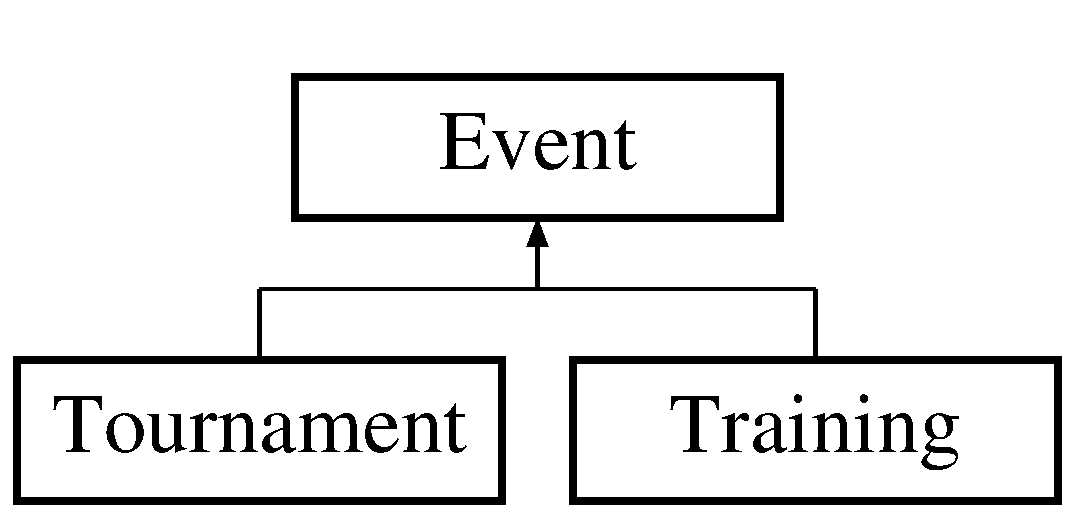
\includegraphics[height=2.000000cm]{class_event}
\end{center}
\end{figure}
\subsection*{Public Member Functions}
\begin{DoxyCompactItemize}
\item 
\hyperlink{class_event_a5a40dd4708297f7031e29b39e039ae10}{Event} ()
\begin{DoxyCompactList}\small\item\em Default Constructor. \end{DoxyCompactList}\item 
virtual \hyperlink{class_event_ab864fd85c758006c42cd7a1b3369b483}{$\sim$\+Event} ()
\begin{DoxyCompactList}\small\item\em Destructor. \end{DoxyCompactList}\item 
\hyperlink{class_event_aa79f43b0c42280875280ec071aa2eea1}{Event} (const \hyperlink{class_event}{Event} \&ev)
\begin{DoxyCompactList}\small\item\em Copy Constructor. \end{DoxyCompactList}\item 
\hyperlink{class_event_ad13c7b9652c4e3ab546d86406097d23a}{Event} (\hyperlink{class_date}{Date} day)
\begin{DoxyCompactList}\small\item\em Contructor. \end{DoxyCompactList}\item 
\hyperlink{class_event}{Event} \& \hyperlink{class_event_a8115e592203a26166924dcae5b064e06}{operator=} (const \hyperlink{class_event}{Event} \&ev)
\begin{DoxyCompactList}\small\item\em operator= Used to copy contents of one \hyperlink{class_event}{Event} to other \end{DoxyCompactList}\item 
vector$<$ string $>$ \hyperlink{class_event_a67677233149ff7e2ebe038d3cfa35223}{get\+Presences} () const
\begin{DoxyCompactList}\small\item\em Gets the member variable presences. \end{DoxyCompactList}\item 
\hyperlink{class_date}{Date} \hyperlink{class_event_a9c016f59ee7116b2397a4823911e1a65}{get\+Day} () const
\begin{DoxyCompactList}\small\item\em Gets the member variable day. \end{DoxyCompactList}\item 
void \hyperlink{class_event_a7e9fa73e721c69bdf05b894ec3178e9b}{set\+Day} (\hyperlink{class_date}{Date} day)
\begin{DoxyCompactList}\small\item\em Changes the value of member variable day. \end{DoxyCompactList}\item 
void \hyperlink{class_event_a2e63387b12ece5fc8b38c6b1142df219}{set\+Presences} (vector$<$ string $>$ presences)
\begin{DoxyCompactList}\small\item\em Changes the value of member variable presences. \end{DoxyCompactList}\item 
void \hyperlink{class_event_a3efb47d783affa24203f4ba13b355c56}{add\+Presence} (string presence)
\begin{DoxyCompactList}\small\item\em Adds a name of \hyperlink{class_player}{Player} to member variable presences. \end{DoxyCompactList}\item 
virtual bool \hyperlink{class_event_a08af9b350f32520dca26d552d6f415b2}{Istraining} () const =0
\begin{DoxyCompactList}\small\item\em Used to check if this \hyperlink{class_event}{Event} is a Trainings. \end{DoxyCompactList}\item 
virtual bool \hyperlink{class_event_add36e9739215f6744040c11de50b26b7}{is\+Game} () const =0
\begin{DoxyCompactList}\small\item\em Used to check if this \hyperlink{class_event}{Event} is a game (only possible in \hyperlink{class_training}{Training}) \end{DoxyCompactList}\item 
virtual unsigned int \hyperlink{class_event_ab267b8e94c78ca51636792d75101acb5}{get\+Rank} () const =0
\begin{DoxyCompactList}\small\item\em Used get rank of team in \hyperlink{class_tournament}{Tournament}. \end{DoxyCompactList}\item 
virtual bool \hyperlink{class_event_ad1a1a9cb471d664a2ca99effc102259b}{is\+Major} () const =0
\begin{DoxyCompactList}\small\item\em Used to check if this \hyperlink{class_event}{Event} is a major \hyperlink{class_tournament}{Tournament} (only possible in \hyperlink{class_tournament}{Tournament}) \end{DoxyCompactList}\item 
virtual vector$<$ pair$<$ pair$<$ unsigned int, unsigned int $>$, string $>$ $>$ \hyperlink{class_event_a9d29f8c725da32b5fbf70ccf7961f02b}{get\+Results} () const =0
\begin{DoxyCompactList}\small\item\em Get the results of the \hyperlink{class_level}{Level} in a \hyperlink{class_tournament}{Tournament} (only possible in \hyperlink{class_tournament}{Tournament}) \end{DoxyCompactList}\item 
virtual void \hyperlink{class_event_a5ddb261642035be78677d668f9238339}{set\+Results} (vector$<$ pair$<$ pair$<$ unsigned int, unsigned int $>$, string $>$$>$ results)=0
\begin{DoxyCompactList}\small\item\em Changes the results of the \hyperlink{class_level}{Level} in a \hyperlink{class_tournament}{Tournament} (only possible in \hyperlink{class_tournament}{Tournament}) \end{DoxyCompactList}\item 
virtual void \hyperlink{class_event_a5bccaba301e9038957ec4138df404524}{set\+Rank} (unsigned int rank)=0
\begin{DoxyCompactList}\small\item\em Changes the rank of the \hyperlink{class_level}{Level} in a \hyperlink{class_tournament}{Tournament} (only possible in \hyperlink{class_tournament}{Tournament}) \end{DoxyCompactList}\item 
virtual void \hyperlink{class_event_af53c2db83404a045087a271ed3c2604f}{show} () const =0
\begin{DoxyCompactList}\small\item\em Printf the \hyperlink{class_event}{Event} in the screen, output of Trainings different from Tournaments. \end{DoxyCompactList}\item 
virtual void \hyperlink{class_event_a0c263fb7398dc2f0969a2bb22b47a40a}{writetofile} (ostream \&out) const =0
\begin{DoxyCompactList}\small\item\em Writes information about the Evento to an output stream. \end{DoxyCompactList}\item 
bool \hyperlink{class_event_a7bdc01f67b0ebca8feb9650d63c8ff08}{operator$<$} (const \hyperlink{class_event}{Event} \&ev1) const
\begin{DoxyCompactList}\small\item\em Operator $<$ compares two events. \end{DoxyCompactList}\end{DoxyCompactItemize}


\subsection{Detailed Description}
Class to hold information about an event. 

Definition at line 23 of file Event.\+h.



\subsection{Constructor \& Destructor Documentation}
\hypertarget{class_event_a5a40dd4708297f7031e29b39e039ae10}{}\label{class_event_a5a40dd4708297f7031e29b39e039ae10} 
\index{Event@{Event}!Event@{Event}}
\index{Event@{Event}!Event@{Event}}
\subsubsection{\texorpdfstring{Event()}{Event()}\hspace{0.1cm}{\footnotesize\ttfamily [1/3]}}
{\footnotesize\ttfamily Event\+::\+Event (\begin{DoxyParamCaption}{ }\end{DoxyParamCaption})\hspace{0.3cm}{\ttfamily [inline]}}



Default Constructor. 



Definition at line 30 of file Event.\+h.

\hypertarget{class_event_ab864fd85c758006c42cd7a1b3369b483}{}\label{class_event_ab864fd85c758006c42cd7a1b3369b483} 
\index{Event@{Event}!````~Event@{$\sim$\+Event}}
\index{````~Event@{$\sim$\+Event}!Event@{Event}}
\subsubsection{\texorpdfstring{$\sim$\+Event()}{~Event()}}
{\footnotesize\ttfamily virtual Event\+::$\sim$\+Event (\begin{DoxyParamCaption}{ }\end{DoxyParamCaption})\hspace{0.3cm}{\ttfamily [inline]}, {\ttfamily [virtual]}}



Destructor. 



Definition at line 34 of file Event.\+h.

\hypertarget{class_event_aa79f43b0c42280875280ec071aa2eea1}{}\label{class_event_aa79f43b0c42280875280ec071aa2eea1} 
\index{Event@{Event}!Event@{Event}}
\index{Event@{Event}!Event@{Event}}
\subsubsection{\texorpdfstring{Event()}{Event()}\hspace{0.1cm}{\footnotesize\ttfamily [2/3]}}
{\footnotesize\ttfamily Event\+::\+Event (\begin{DoxyParamCaption}\item[{const \hyperlink{class_event}{Event} \&}]{ev }\end{DoxyParamCaption})\hspace{0.3cm}{\ttfamily [inline]}}



Copy Constructor. 


\begin{DoxyParams}{Parameters}
{\em ev} & Object of class \hyperlink{class_event}{Event} to be copied \\
\hline
\end{DoxyParams}


Definition at line 39 of file Event.\+h.

\hypertarget{class_event_ad13c7b9652c4e3ab546d86406097d23a}{}\label{class_event_ad13c7b9652c4e3ab546d86406097d23a} 
\index{Event@{Event}!Event@{Event}}
\index{Event@{Event}!Event@{Event}}
\subsubsection{\texorpdfstring{Event()}{Event()}\hspace{0.1cm}{\footnotesize\ttfamily [3/3]}}
{\footnotesize\ttfamily Event\+::\+Event (\begin{DoxyParamCaption}\item[{\hyperlink{class_date}{Date}}]{day }\end{DoxyParamCaption})\hspace{0.3cm}{\ttfamily [inline]}}



Contructor. 


\begin{DoxyParams}{Parameters}
{\em day} & \hyperlink{class_date}{Date} of the \hyperlink{class_event}{Event} \\
\hline
\end{DoxyParams}


Definition at line 44 of file Event.\+h.



\subsection{Member Function Documentation}
\hypertarget{class_event_a3efb47d783affa24203f4ba13b355c56}{}\label{class_event_a3efb47d783affa24203f4ba13b355c56} 
\index{Event@{Event}!add\+Presence@{add\+Presence}}
\index{add\+Presence@{add\+Presence}!Event@{Event}}
\subsubsection{\texorpdfstring{add\+Presence()}{addPresence()}}
{\footnotesize\ttfamily void Event\+::add\+Presence (\begin{DoxyParamCaption}\item[{string}]{presence }\end{DoxyParamCaption})\hspace{0.3cm}{\ttfamily [inline]}}



Adds a name of \hyperlink{class_player}{Player} to member variable presences. 



Definition at line 73 of file Event.\+h.

\hypertarget{class_event_a9c016f59ee7116b2397a4823911e1a65}{}\label{class_event_a9c016f59ee7116b2397a4823911e1a65} 
\index{Event@{Event}!get\+Day@{get\+Day}}
\index{get\+Day@{get\+Day}!Event@{Event}}
\subsubsection{\texorpdfstring{get\+Day()}{getDay()}}
{\footnotesize\ttfamily \hyperlink{class_date}{Date} Event\+::get\+Day (\begin{DoxyParamCaption}{ }\end{DoxyParamCaption}) const\hspace{0.3cm}{\ttfamily [inline]}}



Gets the member variable day. 

\begin{DoxyReturn}{Returns}
day (member variable) 
\end{DoxyReturn}


Definition at line 61 of file Event.\+h.

\hypertarget{class_event_a67677233149ff7e2ebe038d3cfa35223}{}\label{class_event_a67677233149ff7e2ebe038d3cfa35223} 
\index{Event@{Event}!get\+Presences@{get\+Presences}}
\index{get\+Presences@{get\+Presences}!Event@{Event}}
\subsubsection{\texorpdfstring{get\+Presences()}{getPresences()}}
{\footnotesize\ttfamily vector$<$string$>$ Event\+::get\+Presences (\begin{DoxyParamCaption}{ }\end{DoxyParamCaption}) const\hspace{0.3cm}{\ttfamily [inline]}}



Gets the member variable presences. 

\begin{DoxyReturn}{Returns}
presences (member variable) 
\end{DoxyReturn}


Definition at line 56 of file Event.\+h.

\hypertarget{class_event_ab267b8e94c78ca51636792d75101acb5}{}\label{class_event_ab267b8e94c78ca51636792d75101acb5} 
\index{Event@{Event}!get\+Rank@{get\+Rank}}
\index{get\+Rank@{get\+Rank}!Event@{Event}}
\subsubsection{\texorpdfstring{get\+Rank()}{getRank()}}
{\footnotesize\ttfamily virtual unsigned int Event\+::get\+Rank (\begin{DoxyParamCaption}{ }\end{DoxyParamCaption}) const\hspace{0.3cm}{\ttfamily [pure virtual]}}



Used get rank of team in \hyperlink{class_tournament}{Tournament}. 

\begin{DoxyReturn}{Returns}
\hyperlink{class_tournament}{Tournament} member variable rank or 0 if object is not a \hyperlink{class_tournament}{Tournament}
\end{DoxyReturn}
Pure virtual, to be implemented by derived classes 

Implemented in \hyperlink{class_tournament_ae021dc9d9aa7fb8b18bd065bfccc4b7e}{Tournament}, and \hyperlink{class_training_ada723ff1f8340338a99e720a1b472334}{Training}.

\hypertarget{class_event_a9d29f8c725da32b5fbf70ccf7961f02b}{}\label{class_event_a9d29f8c725da32b5fbf70ccf7961f02b} 
\index{Event@{Event}!get\+Results@{get\+Results}}
\index{get\+Results@{get\+Results}!Event@{Event}}
\subsubsection{\texorpdfstring{get\+Results()}{getResults()}}
{\footnotesize\ttfamily virtual vector$<$pair$<$pair$<$unsigned int, unsigned int$>$, string $>$ $>$ Event\+::get\+Results (\begin{DoxyParamCaption}{ }\end{DoxyParamCaption}) const\hspace{0.3cm}{\ttfamily [pure virtual]}}



Get the results of the \hyperlink{class_level}{Level} in a \hyperlink{class_tournament}{Tournament} (only possible in \hyperlink{class_tournament}{Tournament}) 

\begin{DoxyReturn}{Returns}
Vector with results of games and the Clubs played against, or empty if object is not \hyperlink{class_tournament}{Tournament}
\end{DoxyReturn}
Pure virtual, to be implemented by derived classes 

Implemented in \hyperlink{class_tournament_abacd2d5489099f31a9688a7da4d64c40}{Tournament}, and \hyperlink{class_training_aa37e2baeee2b94cb15521e1768b99cc9}{Training}.

\hypertarget{class_event_add36e9739215f6744040c11de50b26b7}{}\label{class_event_add36e9739215f6744040c11de50b26b7} 
\index{Event@{Event}!is\+Game@{is\+Game}}
\index{is\+Game@{is\+Game}!Event@{Event}}
\subsubsection{\texorpdfstring{is\+Game()}{isGame()}}
{\footnotesize\ttfamily virtual bool Event\+::is\+Game (\begin{DoxyParamCaption}{ }\end{DoxyParamCaption}) const\hspace{0.3cm}{\ttfamily [pure virtual]}}



Used to check if this \hyperlink{class_event}{Event} is a game (only possible in \hyperlink{class_training}{Training}) 

\begin{DoxyReturn}{Returns}
true if \hyperlink{class_event}{Event} is a game, false if not or if not a \hyperlink{class_training}{Training}
\end{DoxyReturn}
Pure virtual, to be implemented by derived classes 

Implemented in \hyperlink{class_tournament_a62adb322a6d5268d4ec3e267570ff4ed}{Tournament}, and \hyperlink{class_training_a55530cc22aa771cf3e452c7158b5396e}{Training}.

\hypertarget{class_event_ad1a1a9cb471d664a2ca99effc102259b}{}\label{class_event_ad1a1a9cb471d664a2ca99effc102259b} 
\index{Event@{Event}!is\+Major@{is\+Major}}
\index{is\+Major@{is\+Major}!Event@{Event}}
\subsubsection{\texorpdfstring{is\+Major()}{isMajor()}}
{\footnotesize\ttfamily virtual bool Event\+::is\+Major (\begin{DoxyParamCaption}{ }\end{DoxyParamCaption}) const\hspace{0.3cm}{\ttfamily [pure virtual]}}



Used to check if this \hyperlink{class_event}{Event} is a major \hyperlink{class_tournament}{Tournament} (only possible in \hyperlink{class_tournament}{Tournament}) 

\begin{DoxyReturn}{Returns}
true if \hyperlink{class_event}{Event} is a major \hyperlink{class_tournament}{Tournament}, false if not or if not a \hyperlink{class_training}{Training}
\end{DoxyReturn}
Pure virtual, to be implemented by derived classes 

Implemented in \hyperlink{class_tournament_af733baa05b3ae1465d6b5271929b5061}{Tournament}, and \hyperlink{class_training_aaf1c4d96664a16ca141dd5a3582f9426}{Training}.

\hypertarget{class_event_a08af9b350f32520dca26d552d6f415b2}{}\label{class_event_a08af9b350f32520dca26d552d6f415b2} 
\index{Event@{Event}!Istraining@{Istraining}}
\index{Istraining@{Istraining}!Event@{Event}}
\subsubsection{\texorpdfstring{Istraining()}{Istraining()}}
{\footnotesize\ttfamily virtual bool Event\+::\+Istraining (\begin{DoxyParamCaption}{ }\end{DoxyParamCaption}) const\hspace{0.3cm}{\ttfamily [pure virtual]}}



Used to check if this \hyperlink{class_event}{Event} is a Trainings. 

\begin{DoxyReturn}{Returns}
true if \hyperlink{class_event}{Event} is Trainings, false if not
\end{DoxyReturn}
Pure virtual, to be implemented by derived classes 

Implemented in \hyperlink{class_tournament_ab6fde765568ea9779fc10f0f2811c163}{Tournament}, and \hyperlink{class_training_ab70fe087f382d0de9dca69ce519be91e}{Training}.

\hypertarget{class_event_a7bdc01f67b0ebca8feb9650d63c8ff08}{}\label{class_event_a7bdc01f67b0ebca8feb9650d63c8ff08} 
\index{Event@{Event}!operator$<$@{operator$<$}}
\index{operator$<$@{operator$<$}!Event@{Event}}
\subsubsection{\texorpdfstring{operator$<$()}{operator<()}}
{\footnotesize\ttfamily bool Event\+::operator$<$ (\begin{DoxyParamCaption}\item[{const \hyperlink{class_event}{Event} \&}]{ev1 }\end{DoxyParamCaption}) const\hspace{0.3cm}{\ttfamily [inline]}}



Operator $<$ compares two events. 


\begin{DoxyParams}{Parameters}
{\em ev1} & \hyperlink{class_event}{Event} to be used for comparison \\
\hline
\end{DoxyParams}
\begin{DoxyReturn}{Returns}
True if $\ast$this is sooner than parameter ev1
\end{DoxyReturn}
The Events are compared by \hyperlink{class_date}{Date} such that an \hyperlink{class_event}{Event} is bigger than another if it happened later 

Definition at line 134 of file Event.\+h.

\hypertarget{class_event_a8115e592203a26166924dcae5b064e06}{}\label{class_event_a8115e592203a26166924dcae5b064e06} 
\index{Event@{Event}!operator=@{operator=}}
\index{operator=@{operator=}!Event@{Event}}
\subsubsection{\texorpdfstring{operator=()}{operator=()}}
{\footnotesize\ttfamily \hyperlink{class_event}{Event}\& Event\+::operator= (\begin{DoxyParamCaption}\item[{const \hyperlink{class_event}{Event} \&}]{ev }\end{DoxyParamCaption})\hspace{0.3cm}{\ttfamily [inline]}}



operator= Used to copy contents of one \hyperlink{class_event}{Event} to other 


\begin{DoxyParams}{Parameters}
{\em ev} & Object of \hyperlink{class_event}{Event} to be copied \\
\hline
\end{DoxyParams}
\begin{DoxyReturn}{Returns}
Object of \hyperlink{class_event}{Event} into which parameter ev was copied
\end{DoxyReturn}
Copies all of the member variables 

Definition at line 51 of file Event.\+h.

\hypertarget{class_event_a7e9fa73e721c69bdf05b894ec3178e9b}{}\label{class_event_a7e9fa73e721c69bdf05b894ec3178e9b} 
\index{Event@{Event}!set\+Day@{set\+Day}}
\index{set\+Day@{set\+Day}!Event@{Event}}
\subsubsection{\texorpdfstring{set\+Day()}{setDay()}}
{\footnotesize\ttfamily void Event\+::set\+Day (\begin{DoxyParamCaption}\item[{\hyperlink{class_date}{Date}}]{day }\end{DoxyParamCaption})\hspace{0.3cm}{\ttfamily [inline]}}



Changes the value of member variable day. 



Definition at line 65 of file Event.\+h.

\hypertarget{class_event_a2e63387b12ece5fc8b38c6b1142df219}{}\label{class_event_a2e63387b12ece5fc8b38c6b1142df219} 
\index{Event@{Event}!set\+Presences@{set\+Presences}}
\index{set\+Presences@{set\+Presences}!Event@{Event}}
\subsubsection{\texorpdfstring{set\+Presences()}{setPresences()}}
{\footnotesize\ttfamily void Event\+::set\+Presences (\begin{DoxyParamCaption}\item[{vector$<$ string $>$}]{presences }\end{DoxyParamCaption})\hspace{0.3cm}{\ttfamily [inline]}}



Changes the value of member variable presences. 



Definition at line 69 of file Event.\+h.

\hypertarget{class_event_a5bccaba301e9038957ec4138df404524}{}\label{class_event_a5bccaba301e9038957ec4138df404524} 
\index{Event@{Event}!set\+Rank@{set\+Rank}}
\index{set\+Rank@{set\+Rank}!Event@{Event}}
\subsubsection{\texorpdfstring{set\+Rank()}{setRank()}}
{\footnotesize\ttfamily virtual void Event\+::set\+Rank (\begin{DoxyParamCaption}\item[{unsigned int}]{rank }\end{DoxyParamCaption})\hspace{0.3cm}{\ttfamily [pure virtual]}}



Changes the rank of the \hyperlink{class_level}{Level} in a \hyperlink{class_tournament}{Tournament} (only possible in \hyperlink{class_tournament}{Tournament}) 


\begin{DoxyParams}{Parameters}
{\em rank} & The rank of the \hyperlink{class_level}{Level}\\
\hline
\end{DoxyParams}
Pure virtual, to be implemented by derived classes 

Implemented in \hyperlink{class_tournament_a724f8fb0c0507975b6bb4817d8b5de7d}{Tournament}, and \hyperlink{class_training_a15d38322bd6a2ee8e17441bd4798b236}{Training}.

\hypertarget{class_event_a5ddb261642035be78677d668f9238339}{}\label{class_event_a5ddb261642035be78677d668f9238339} 
\index{Event@{Event}!set\+Results@{set\+Results}}
\index{set\+Results@{set\+Results}!Event@{Event}}
\subsubsection{\texorpdfstring{set\+Results()}{setResults()}}
{\footnotesize\ttfamily virtual void Event\+::set\+Results (\begin{DoxyParamCaption}\item[{vector$<$ pair$<$ pair$<$ unsigned int, unsigned int $>$, string $>$$>$}]{results }\end{DoxyParamCaption})\hspace{0.3cm}{\ttfamily [pure virtual]}}



Changes the results of the \hyperlink{class_level}{Level} in a \hyperlink{class_tournament}{Tournament} (only possible in \hyperlink{class_tournament}{Tournament}) 


\begin{DoxyParams}{Parameters}
{\em results} & The results of the \hyperlink{class_level}{Level}\\
\hline
\end{DoxyParams}
Pure virtual, to be implemented by derived classes 

Implemented in \hyperlink{class_tournament_acab9ee32169ba590f4ffdb5b59b28a86}{Tournament}, and \hyperlink{class_training_ad587b59c44a6e95a4e52f3d3f6b89480}{Training}.

\hypertarget{class_event_af53c2db83404a045087a271ed3c2604f}{}\label{class_event_af53c2db83404a045087a271ed3c2604f} 
\index{Event@{Event}!show@{show}}
\index{show@{show}!Event@{Event}}
\subsubsection{\texorpdfstring{show()}{show()}}
{\footnotesize\ttfamily virtual void Event\+::show (\begin{DoxyParamCaption}{ }\end{DoxyParamCaption}) const\hspace{0.3cm}{\ttfamily [pure virtual]}}



Printf the \hyperlink{class_event}{Event} in the screen, output of Trainings different from Tournaments. 

Pure virtual, to be implemented by derived classes 

Implemented in \hyperlink{class_tournament_a35bd5292194edb5d5c220838b68cda75}{Tournament}, and \hyperlink{class_training_a9391fa1f4862855341d6243e75f9efef}{Training}.

\hypertarget{class_event_a0c263fb7398dc2f0969a2bb22b47a40a}{}\label{class_event_a0c263fb7398dc2f0969a2bb22b47a40a} 
\index{Event@{Event}!writetofile@{writetofile}}
\index{writetofile@{writetofile}!Event@{Event}}
\subsubsection{\texorpdfstring{writetofile()}{writetofile()}}
{\footnotesize\ttfamily virtual void Event\+::writetofile (\begin{DoxyParamCaption}\item[{ostream \&}]{out }\end{DoxyParamCaption}) const\hspace{0.3cm}{\ttfamily [pure virtual]}}



Writes information about the Evento to an output stream. 


\begin{DoxyParams}{Parameters}
{\em out} & Output Stream to write to\\
\hline
\end{DoxyParams}
Used to output \hyperlink{class_event}{Event} information on a text file 

Implemented in \hyperlink{class_tournament_a4aa375c287d890b9117a91058dcffb0c}{Tournament}, and \hyperlink{class_training_a1755abc9faafbe06fb2825cb5f879016}{Training}.



The documentation for this class was generated from the following file\+:\begin{DoxyCompactItemize}
\item 
/home/oco/\+Documents/\+Cprojects/\+Athletes/projecto -\/ V2/\+Headers/\hyperlink{_event_8h}{Event.\+h}\end{DoxyCompactItemize}

\hypertarget{structhash_funcs}{}\section{hash\+Funcs Struct Reference}
\label{structhash_funcs}\index{hash\+Funcs@{hash\+Funcs}}


Functions used in \hyperlink{class_club}{Club} member variable future\+\_\+birthdays Chained Hash-\/\+Table.  




{\ttfamily \#include $<$Club.\+h$>$}

\subsection*{Public Member Functions}
\begin{DoxyCompactItemize}
\item 
size\+\_\+t \hyperlink{structhash_funcs_a521b1888977a80fcd935e8e03c09d916}{operator()} (const \hyperlink{class_player}{Player} $\ast$p1) const
\begin{DoxyCompactList}\small\item\em Computates the difference in days between the birthday date and current date. \end{DoxyCompactList}\item 
bool \hyperlink{structhash_funcs_a9e171ebf004435ea1d1ceb8a30f6a954}{operator()} (const \hyperlink{class_player}{Player} $\ast$p1, const \hyperlink{class_player}{Player} $\ast$p2) const
\begin{DoxyCompactList}\small\item\em Compares two pointer to players to see if the Players they are pointing is the same (needed for hash table) \end{DoxyCompactList}\end{DoxyCompactItemize}


\subsection{Detailed Description}
Functions used in \hyperlink{class_club}{Club} member variable future\+\_\+birthdays Chained Hash-\/\+Table. 

Definition at line 37 of file Club.\+h.



\subsection{Member Function Documentation}
\hypertarget{structhash_funcs_a521b1888977a80fcd935e8e03c09d916}{}\label{structhash_funcs_a521b1888977a80fcd935e8e03c09d916} 
\index{hash\+Funcs@{hash\+Funcs}!operator()@{operator()}}
\index{operator()@{operator()}!hash\+Funcs@{hash\+Funcs}}
\subsubsection{\texorpdfstring{operator()()}{operator()()}\hspace{0.1cm}{\footnotesize\ttfamily [1/2]}}
{\footnotesize\ttfamily size\+\_\+t hash\+Funcs\+::operator() (\begin{DoxyParamCaption}\item[{const \hyperlink{class_player}{Player} $\ast$}]{p1 }\end{DoxyParamCaption}) const\hspace{0.3cm}{\ttfamily [inline]}}



Computates the difference in days between the birthday date and current date. 


\begin{DoxyParams}{Parameters}
{\em p1} & Used has hash function \\
\hline
\end{DoxyParams}
\begin{DoxyReturn}{Returns}
If birthday $>$ current date returns number of days, else returns -\/1 
\end{DoxyReturn}


Definition at line 44 of file Club.\+h.

\hypertarget{structhash_funcs_a9e171ebf004435ea1d1ceb8a30f6a954}{}\label{structhash_funcs_a9e171ebf004435ea1d1ceb8a30f6a954} 
\index{hash\+Funcs@{hash\+Funcs}!operator()@{operator()}}
\index{operator()@{operator()}!hash\+Funcs@{hash\+Funcs}}
\subsubsection{\texorpdfstring{operator()()}{operator()()}\hspace{0.1cm}{\footnotesize\ttfamily [2/2]}}
{\footnotesize\ttfamily bool hash\+Funcs\+::operator() (\begin{DoxyParamCaption}\item[{const \hyperlink{class_player}{Player} $\ast$}]{p1,  }\item[{const \hyperlink{class_player}{Player} $\ast$}]{p2 }\end{DoxyParamCaption}) const\hspace{0.3cm}{\ttfamily [inline]}}



Compares two pointer to players to see if the Players they are pointing is the same (needed for hash table) 


\begin{DoxyParams}{Parameters}
{\em p1} & Pointer to \hyperlink{class_player}{Player} 1 \\
\hline
{\em p2} & Pointer to \hyperlink{class_player}{Player} 2 Used as compare function for hash table used. We are only interested if the day and month are equal, the year may be different \\
\hline
\end{DoxyParams}
\begin{DoxyReturn}{Returns}
1 if Players are the same , 0 if not 
\end{DoxyReturn}


Definition at line 55 of file Club.\+h.



The documentation for this struct was generated from the following file\+:\begin{DoxyCompactItemize}
\item 
/home/oco/\+Documents/\+Cprojects/\+Athletes/projecto -\/ V2/\+Headers/\hyperlink{_club_8h}{Club.\+h}\end{DoxyCompactItemize}

\hypertarget{class_invalid_date}{}\section{Invalid\+Date Class Reference}
\label{class_invalid_date}\index{Invalid\+Date@{Invalid\+Date}}


Represents an Invalid \hyperlink{class_date}{Date}.  




{\ttfamily \#include $<$exceptions.\+h$>$}

\subsection*{Public Member Functions}
\begin{DoxyCompactItemize}
\item 
\hyperlink{class_invalid_date_aec8bd136d7adb6bccf44bf6d9f078a40}{Invalid\+Date} (unsigned int day, unsigned int month, unsigned int year)
\begin{DoxyCompactList}\small\item\em Full-\/\+Constructor. \end{DoxyCompactList}\item 
void \hyperlink{class_invalid_date_a665b9e90ec4cab29d400010cd73bb8ed}{show} () const
\begin{DoxyCompactList}\small\item\em Prints the date on the screen. \end{DoxyCompactList}\end{DoxyCompactItemize}


\subsection{Detailed Description}
Represents an Invalid \hyperlink{class_date}{Date}. 

Definition at line 25 of file exceptions.\+h.



\subsection{Constructor \& Destructor Documentation}
\hypertarget{class_invalid_date_aec8bd136d7adb6bccf44bf6d9f078a40}{}\label{class_invalid_date_aec8bd136d7adb6bccf44bf6d9f078a40} 
\index{Invalid\+Date@{Invalid\+Date}!Invalid\+Date@{Invalid\+Date}}
\index{Invalid\+Date@{Invalid\+Date}!Invalid\+Date@{Invalid\+Date}}
\subsubsection{\texorpdfstring{Invalid\+Date()}{InvalidDate()}}
{\footnotesize\ttfamily Invalid\+Date\+::\+Invalid\+Date (\begin{DoxyParamCaption}\item[{unsigned int}]{day,  }\item[{unsigned int}]{month,  }\item[{unsigned int}]{year }\end{DoxyParamCaption})\hspace{0.3cm}{\ttfamily [inline]}}



Full-\/\+Constructor. 


\begin{DoxyParams}{Parameters}
{\em day} & Day of the \hyperlink{class_date}{Date} \\
\hline
{\em month} & Month of the \hyperlink{class_date}{Date} \\
\hline
{\em year} & Year of the \hyperlink{class_date}{Date} \\
\hline
\end{DoxyParams}


Definition at line 36 of file exceptions.\+h.



\subsection{Member Function Documentation}
\hypertarget{class_invalid_date_a665b9e90ec4cab29d400010cd73bb8ed}{}\label{class_invalid_date_a665b9e90ec4cab29d400010cd73bb8ed} 
\index{Invalid\+Date@{Invalid\+Date}!show@{show}}
\index{show@{show}!Invalid\+Date@{Invalid\+Date}}
\subsubsection{\texorpdfstring{show()}{show()}}
{\footnotesize\ttfamily void Invalid\+Date\+::show (\begin{DoxyParamCaption}{ }\end{DoxyParamCaption}) const\hspace{0.3cm}{\ttfamily [inline]}}



Prints the date on the screen. 



Definition at line 40 of file exceptions.\+h.



The documentation for this class was generated from the following file\+:\begin{DoxyCompactItemize}
\item 
/home/oco/\+Documents/\+Cprojects/\+Athletes/projecto -\/ V2/\+Headers/\hyperlink{exceptions_8h}{exceptions.\+h}\end{DoxyCompactItemize}

\hypertarget{class_invalid_player}{}\section{Invalid\+Player Class Reference}
\label{class_invalid_player}\index{Invalid\+Player@{Invalid\+Player}}


Represents an Invalid Players.  




{\ttfamily \#include $<$exceptions.\+h$>$}

\subsection*{Public Member Functions}
\begin{DoxyCompactItemize}
\item 
\hyperlink{class_invalid_player_a311099a3c76237e49e448de25aef4a89}{Invalid\+Player} (string name, \hyperlink{class_date}{Date} birth)
\begin{DoxyCompactList}\small\item\em Full-\/\+Constructor. \end{DoxyCompactList}\item 
void \hyperlink{class_invalid_player_a5254e7755b435020a786a2de1c20418f}{show} () const
\begin{DoxyCompactList}\small\item\em Prints the \hyperlink{class_player}{Player} on the screen. \end{DoxyCompactList}\end{DoxyCompactItemize}


\subsection{Detailed Description}
Represents an Invalid Players. 

Definition at line 51 of file exceptions.\+h.



\subsection{Constructor \& Destructor Documentation}
\hypertarget{class_invalid_player_a311099a3c76237e49e448de25aef4a89}{}\label{class_invalid_player_a311099a3c76237e49e448de25aef4a89} 
\index{Invalid\+Player@{Invalid\+Player}!Invalid\+Player@{Invalid\+Player}}
\index{Invalid\+Player@{Invalid\+Player}!Invalid\+Player@{Invalid\+Player}}
\subsubsection{\texorpdfstring{Invalid\+Player()}{InvalidPlayer()}}
{\footnotesize\ttfamily Invalid\+Player\+::\+Invalid\+Player (\begin{DoxyParamCaption}\item[{string}]{name,  }\item[{\hyperlink{class_date}{Date}}]{birth }\end{DoxyParamCaption})}



Full-\/\+Constructor. 


\begin{DoxyParams}{Parameters}
{\em name} & Name of \hyperlink{class_player}{Player} \\
\hline
{\em birth} & Birthday of \hyperlink{class_player}{Player} \\
\hline
\end{DoxyParams}


Definition at line 6 of file exceptions.\+cpp.



\subsection{Member Function Documentation}
\hypertarget{class_invalid_player_a5254e7755b435020a786a2de1c20418f}{}\label{class_invalid_player_a5254e7755b435020a786a2de1c20418f} 
\index{Invalid\+Player@{Invalid\+Player}!show@{show}}
\index{show@{show}!Invalid\+Player@{Invalid\+Player}}
\subsubsection{\texorpdfstring{show()}{show()}}
{\footnotesize\ttfamily void Invalid\+Player\+::show (\begin{DoxyParamCaption}{ }\end{DoxyParamCaption}) const}



Prints the \hyperlink{class_player}{Player} on the screen. 



Definition at line 11 of file exceptions.\+cpp.



The documentation for this class was generated from the following files\+:\begin{DoxyCompactItemize}
\item 
/home/oco/\+Documents/\+Cprojects/\+Athletes/projecto -\/ V2/\+Headers/\hyperlink{exceptions_8h}{exceptions.\+h}\item 
/home/oco/\+Documents/\+Cprojects/\+Athletes/projecto -\/ V2/\+Source/\hyperlink{exceptions_8cpp}{exceptions.\+cpp}\end{DoxyCompactItemize}

\hypertarget{class_juniors}{}\section{Juniors Class Reference}
\label{class_juniors}\index{Juniors@{Juniors}}


Holds all the information about the \hyperlink{class_level}{Level} \hyperlink{class_juniors}{Juniors}.  




{\ttfamily \#include $<$Juniors.\+h$>$}

Inheritance diagram for Juniors\+:\begin{figure}[H]
\begin{center}
\leavevmode
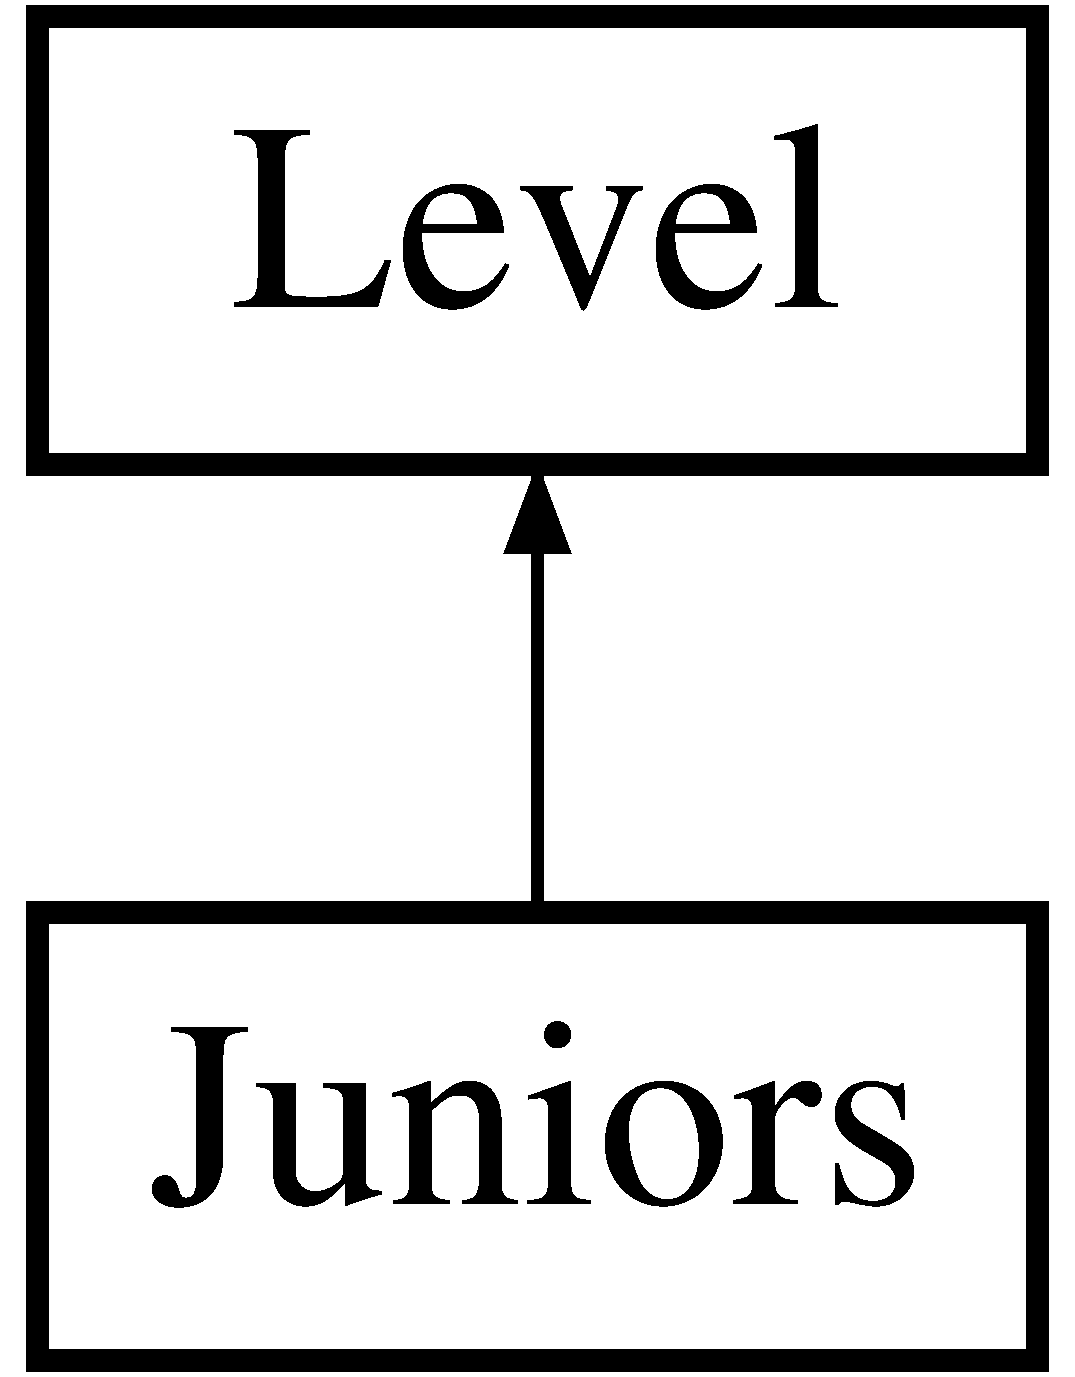
\includegraphics[height=2.000000cm]{class_juniors}
\end{center}
\end{figure}
\subsection*{Public Member Functions}
\begin{DoxyCompactItemize}
\item 
\hyperlink{class_juniors_a36519a818f54755dfd1bd14e15b4fcea}{Juniors} ()
\begin{DoxyCompactList}\small\item\em Default Constructor. \end{DoxyCompactList}\item 
\hyperlink{class_juniors_ae9087dae0157d9a4539f5fc7e68e7478}{$\sim$\+Juniors} ()
\begin{DoxyCompactList}\small\item\em Destructor. \end{DoxyCompactList}\item 
\hyperlink{class_juniors_ab9b00b26e59661ee5aee18a3a6beb53c}{Juniors} (const \hyperlink{class_juniors}{Juniors} \&juniors)
\begin{DoxyCompactList}\small\item\em Copy Constructor. \end{DoxyCompactList}\item 
\hyperlink{class_juniors}{Juniors} \& \hyperlink{class_juniors_adf648456072b60a7f99973c764c01c85}{operator=} (const \hyperlink{class_juniors}{Juniors} \&juniors)
\begin{DoxyCompactList}\small\item\em Copy Operator. \end{DoxyCompactList}\item 
virtual unsigned int \hyperlink{class_juniors_a98c28047a2d5ff2b14651ee9eccfd2b6}{get\+Max\+Age} ()
\begin{DoxyCompactList}\small\item\em Gets the member variable age\+\_\+max. \end{DoxyCompactList}\item 
virtual unsigned int \hyperlink{class_juniors_a3110bdbaa344b2bfefa2ddcb8be8d7c6}{get\+Min\+Age} ()
\begin{DoxyCompactList}\small\item\em Gets the member variable age\+\_\+min. \end{DoxyCompactList}\item 
virtual bool \hyperlink{class_juniors_a23915dab5b0c30a978f08a653483db53}{add\+Player} (\hyperlink{class_player}{Player} $\ast$player)
\begin{DoxyCompactList}\small\item\em Adds a new \hyperlink{class_player}{Player} to this \hyperlink{class_level}{Level}. \end{DoxyCompactList}\item 
virtual void \hyperlink{class_juniors_aa312c32ccc0c9d3193036c20849b8669}{showplayers} () const
\begin{DoxyCompactList}\small\item\em Outputs the Players of this \hyperlink{class_level}{Level} on the screen. \end{DoxyCompactList}\item 
virtual void \hyperlink{class_juniors_ad74d069390fffeda607de3584a0453de}{showtrainings} () const
\begin{DoxyCompactList}\small\item\em Outputs the Trainings of this \hyperlink{class_level}{Level} on the screen. \end{DoxyCompactList}\item 
virtual void \hyperlink{class_juniors_a05afe7596b708ad635ac709499e66bc1}{showtournaments} () const
\begin{DoxyCompactList}\small\item\em Outputs the Tournaments of this \hyperlink{class_level}{Level} on the screen. \end{DoxyCompactList}\item 
virtual vector$<$ string $>$ \hyperlink{class_juniors_ace1da8267f2a92dbfb9e27f7b6b95d26}{get\+Call} (unsigned int size)
\begin{DoxyCompactList}\small\item\em Gets names of players to be called to a \hyperlink{class_tournament}{Tournament}. \end{DoxyCompactList}\end{DoxyCompactItemize}


\subsection{Detailed Description}
Holds all the information about the \hyperlink{class_level}{Level} \hyperlink{class_juniors}{Juniors}. 

Definition at line 23 of file Juniors.\+h.



\subsection{Constructor \& Destructor Documentation}
\hypertarget{class_juniors_a36519a818f54755dfd1bd14e15b4fcea}{}\label{class_juniors_a36519a818f54755dfd1bd14e15b4fcea} 
\index{Juniors@{Juniors}!Juniors@{Juniors}}
\index{Juniors@{Juniors}!Juniors@{Juniors}}
\subsubsection{\texorpdfstring{Juniors()}{Juniors()}\hspace{0.1cm}{\footnotesize\ttfamily [1/2]}}
{\footnotesize\ttfamily Juniors\+::\+Juniors (\begin{DoxyParamCaption}{ }\end{DoxyParamCaption})\hspace{0.3cm}{\ttfamily [inline]}}



Default Constructor. 



Definition at line 29 of file Juniors.\+h.

\hypertarget{class_juniors_ae9087dae0157d9a4539f5fc7e68e7478}{}\label{class_juniors_ae9087dae0157d9a4539f5fc7e68e7478} 
\index{Juniors@{Juniors}!````~Juniors@{$\sim$\+Juniors}}
\index{````~Juniors@{$\sim$\+Juniors}!Juniors@{Juniors}}
\subsubsection{\texorpdfstring{$\sim$\+Juniors()}{~Juniors()}}
{\footnotesize\ttfamily Juniors\+::$\sim$\+Juniors (\begin{DoxyParamCaption}{ }\end{DoxyParamCaption})\hspace{0.3cm}{\ttfamily [inline]}}



Destructor. 



Definition at line 33 of file Juniors.\+h.

\hypertarget{class_juniors_ab9b00b26e59661ee5aee18a3a6beb53c}{}\label{class_juniors_ab9b00b26e59661ee5aee18a3a6beb53c} 
\index{Juniors@{Juniors}!Juniors@{Juniors}}
\index{Juniors@{Juniors}!Juniors@{Juniors}}
\subsubsection{\texorpdfstring{Juniors()}{Juniors()}\hspace{0.1cm}{\footnotesize\ttfamily [2/2]}}
{\footnotesize\ttfamily Juniors\+::\+Juniors (\begin{DoxyParamCaption}\item[{const \hyperlink{class_juniors}{Juniors} \&}]{juniors }\end{DoxyParamCaption})\hspace{0.3cm}{\ttfamily [inline]}}



Copy Constructor. 


\begin{DoxyParams}{Parameters}
{\em juniors} & Object of class to be copied \\
\hline
\end{DoxyParams}


Definition at line 38 of file Juniors.\+h.



\subsection{Member Function Documentation}
\hypertarget{class_juniors_a23915dab5b0c30a978f08a653483db53}{}\label{class_juniors_a23915dab5b0c30a978f08a653483db53} 
\index{Juniors@{Juniors}!add\+Player@{add\+Player}}
\index{add\+Player@{add\+Player}!Juniors@{Juniors}}
\subsubsection{\texorpdfstring{add\+Player()}{addPlayer()}}
{\footnotesize\ttfamily bool Juniors\+::add\+Player (\begin{DoxyParamCaption}\item[{\hyperlink{class_player}{Player} $\ast$}]{player }\end{DoxyParamCaption})\hspace{0.3cm}{\ttfamily [virtual]}}



Adds a new \hyperlink{class_player}{Player} to this \hyperlink{class_level}{Level}. 


\begin{DoxyParams}{Parameters}
{\em player} & Pointer to \hyperlink{class_player}{Player} to be added \\
\hline
\end{DoxyParams}
\begin{DoxyReturn}{Returns}
true if it was added successfuly, false if not 
\end{DoxyReturn}


Reimplemented from \hyperlink{class_level_a66290778fa4bcd2f29b9ff3e605b2902}{Level}.



Definition at line 13 of file Juniors.\+cpp.

\hypertarget{class_juniors_ace1da8267f2a92dbfb9e27f7b6b95d26}{}\label{class_juniors_ace1da8267f2a92dbfb9e27f7b6b95d26} 
\index{Juniors@{Juniors}!get\+Call@{get\+Call}}
\index{get\+Call@{get\+Call}!Juniors@{Juniors}}
\subsubsection{\texorpdfstring{get\+Call()}{getCall()}}
{\footnotesize\ttfamily vector$<$ string $>$ Juniors\+::get\+Call (\begin{DoxyParamCaption}\item[{unsigned int}]{size }\end{DoxyParamCaption})\hspace{0.3cm}{\ttfamily [virtual]}}



Gets names of players to be called to a \hyperlink{class_tournament}{Tournament}. 


\begin{DoxyParams}{Parameters}
{\em size} & How many players to be called \\
\hline
\end{DoxyParams}
\begin{DoxyReturn}{Returns}
Vector with names of Players to be called 
\end{DoxyReturn}


Implements \hyperlink{class_level_ac118b390f16a75b9a0e9df198b3190ad}{Level}.



Definition at line 77 of file Juniors.\+cpp.

\hypertarget{class_juniors_a98c28047a2d5ff2b14651ee9eccfd2b6}{}\label{class_juniors_a98c28047a2d5ff2b14651ee9eccfd2b6} 
\index{Juniors@{Juniors}!get\+Max\+Age@{get\+Max\+Age}}
\index{get\+Max\+Age@{get\+Max\+Age}!Juniors@{Juniors}}
\subsubsection{\texorpdfstring{get\+Max\+Age()}{getMaxAge()}}
{\footnotesize\ttfamily virtual unsigned int Juniors\+::get\+Max\+Age (\begin{DoxyParamCaption}{ }\end{DoxyParamCaption})\hspace{0.3cm}{\ttfamily [inline]}, {\ttfamily [virtual]}}



Gets the member variable age\+\_\+max. 

\begin{DoxyReturn}{Returns}
age\+\_\+max (member variable) 
\end{DoxyReturn}


Implements \hyperlink{class_level_ae7b28ba0cb8d49372c4657fbe42706e1}{Level}.



Definition at line 49 of file Juniors.\+h.

\hypertarget{class_juniors_a3110bdbaa344b2bfefa2ddcb8be8d7c6}{}\label{class_juniors_a3110bdbaa344b2bfefa2ddcb8be8d7c6} 
\index{Juniors@{Juniors}!get\+Min\+Age@{get\+Min\+Age}}
\index{get\+Min\+Age@{get\+Min\+Age}!Juniors@{Juniors}}
\subsubsection{\texorpdfstring{get\+Min\+Age()}{getMinAge()}}
{\footnotesize\ttfamily virtual unsigned int Juniors\+::get\+Min\+Age (\begin{DoxyParamCaption}{ }\end{DoxyParamCaption})\hspace{0.3cm}{\ttfamily [inline]}, {\ttfamily [virtual]}}



Gets the member variable age\+\_\+min. 

\begin{DoxyReturn}{Returns}
age\+\_\+min (member variable) 
\end{DoxyReturn}


Implements \hyperlink{class_level_a161cf8c238fd499c112d90504cb6f587}{Level}.



Definition at line 54 of file Juniors.\+h.

\hypertarget{class_juniors_adf648456072b60a7f99973c764c01c85}{}\label{class_juniors_adf648456072b60a7f99973c764c01c85} 
\index{Juniors@{Juniors}!operator=@{operator=}}
\index{operator=@{operator=}!Juniors@{Juniors}}
\subsubsection{\texorpdfstring{operator=()}{operator=()}}
{\footnotesize\ttfamily \hyperlink{class_juniors}{Juniors}\& Juniors\+::operator= (\begin{DoxyParamCaption}\item[{const \hyperlink{class_juniors}{Juniors} \&}]{juniors }\end{DoxyParamCaption})\hspace{0.3cm}{\ttfamily [inline]}}



Copy Operator. 


\begin{DoxyParams}{Parameters}
{\em juniors} & Object of class to be copied\\
\hline
\end{DoxyParams}
Calls the base class \hyperlink{class_level_a60eb04b65c900ae8dddf3d6251fac7b1}{Level\+::operator=} 

Definition at line 44 of file Juniors.\+h.

\hypertarget{class_juniors_aa312c32ccc0c9d3193036c20849b8669}{}\label{class_juniors_aa312c32ccc0c9d3193036c20849b8669} 
\index{Juniors@{Juniors}!showplayers@{showplayers}}
\index{showplayers@{showplayers}!Juniors@{Juniors}}
\subsubsection{\texorpdfstring{showplayers()}{showplayers()}}
{\footnotesize\ttfamily void Juniors\+::showplayers (\begin{DoxyParamCaption}{ }\end{DoxyParamCaption}) const\hspace{0.3cm}{\ttfamily [virtual]}}



Outputs the Players of this \hyperlink{class_level}{Level} on the screen. 



Reimplemented from \hyperlink{class_level_a40d22b376e72950a07de5e0a9e288029}{Level}.



Definition at line 27 of file Juniors.\+cpp.

\hypertarget{class_juniors_a05afe7596b708ad635ac709499e66bc1}{}\label{class_juniors_a05afe7596b708ad635ac709499e66bc1} 
\index{Juniors@{Juniors}!showtournaments@{showtournaments}}
\index{showtournaments@{showtournaments}!Juniors@{Juniors}}
\subsubsection{\texorpdfstring{showtournaments()}{showtournaments()}}
{\footnotesize\ttfamily void Juniors\+::showtournaments (\begin{DoxyParamCaption}{ }\end{DoxyParamCaption}) const\hspace{0.3cm}{\ttfamily [virtual]}}



Outputs the Tournaments of this \hyperlink{class_level}{Level} on the screen. 



Reimplemented from \hyperlink{class_level_a757c4547f3b8f7c7ecb02c7e0e6cd7c9}{Level}.



Definition at line 43 of file Juniors.\+cpp.

\hypertarget{class_juniors_ad74d069390fffeda607de3584a0453de}{}\label{class_juniors_ad74d069390fffeda607de3584a0453de} 
\index{Juniors@{Juniors}!showtrainings@{showtrainings}}
\index{showtrainings@{showtrainings}!Juniors@{Juniors}}
\subsubsection{\texorpdfstring{showtrainings()}{showtrainings()}}
{\footnotesize\ttfamily void Juniors\+::showtrainings (\begin{DoxyParamCaption}{ }\end{DoxyParamCaption}) const\hspace{0.3cm}{\ttfamily [virtual]}}



Outputs the Trainings of this \hyperlink{class_level}{Level} on the screen. 



Reimplemented from \hyperlink{class_level_a4101cb725b1fd0c0836834c92b190363}{Level}.



Definition at line 35 of file Juniors.\+cpp.



The documentation for this class was generated from the following files\+:\begin{DoxyCompactItemize}
\item 
/home/oco/\+Documents/\+Cprojects/\+Athletes/projecto -\/ V2/\+Headers/\hyperlink{_juniors_8h}{Juniors.\+h}\item 
/home/oco/\+Documents/\+Cprojects/\+Athletes/projecto -\/ V2/\+Source/\hyperlink{_juniors_8cpp}{Juniors.\+cpp}\end{DoxyCompactItemize}

\hypertarget{class_juveniles}{}\section{Juveniles Class Reference}
\label{class_juveniles}\index{Juveniles@{Juveniles}}


Holds all the information about the \hyperlink{class_level}{Level} \hyperlink{class_juveniles}{Juveniles}.  




{\ttfamily \#include $<$Juveniles.\+h$>$}

Inheritance diagram for Juveniles\+:\begin{figure}[H]
\begin{center}
\leavevmode
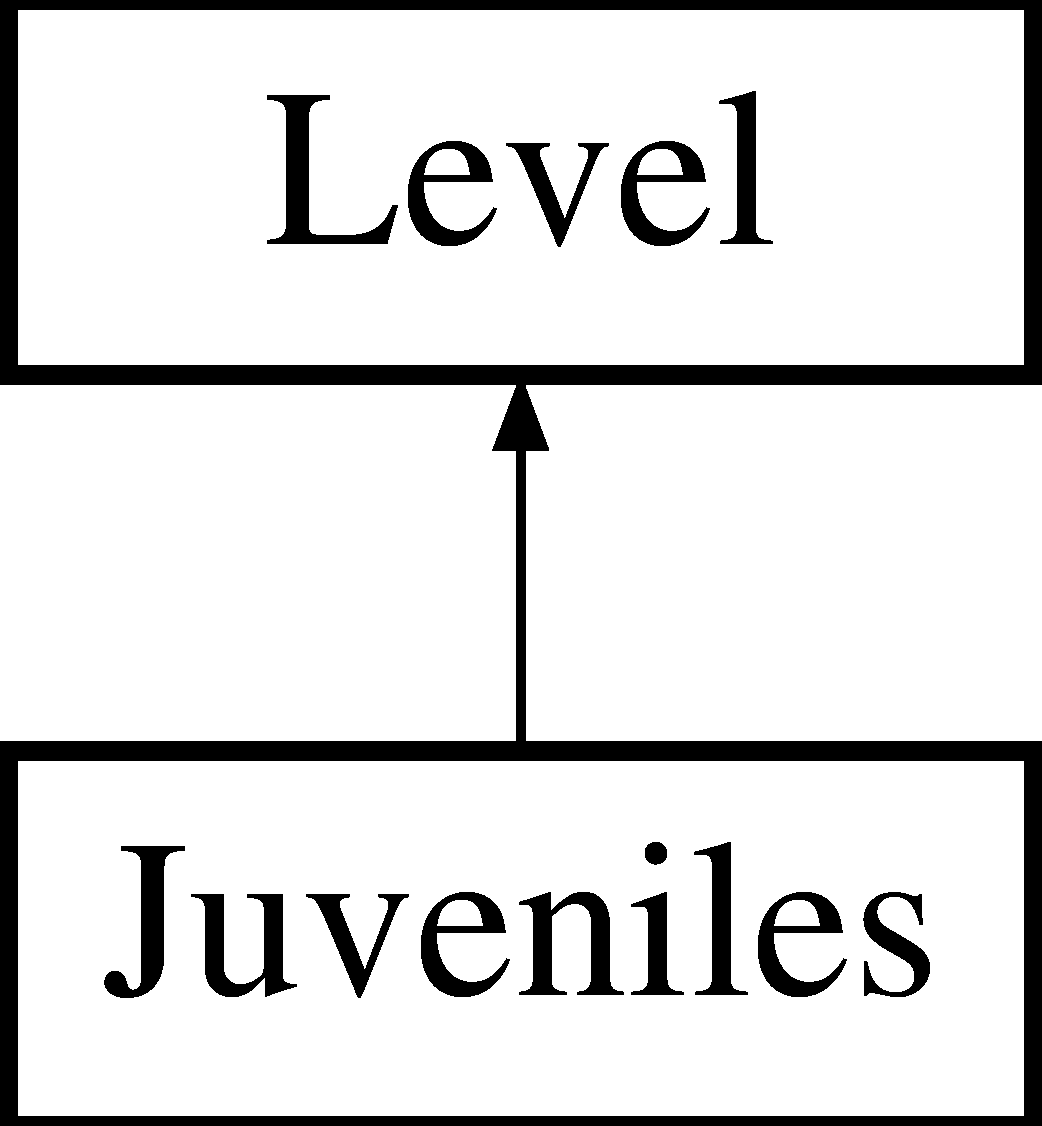
\includegraphics[height=2.000000cm]{class_juveniles}
\end{center}
\end{figure}
\subsection*{Public Member Functions}
\begin{DoxyCompactItemize}
\item 
\hyperlink{class_juveniles_a01be3288bd98fed2069a5a4d230a6a45}{Juveniles} ()
\begin{DoxyCompactList}\small\item\em Default Constructor. \end{DoxyCompactList}\item 
\hyperlink{class_juveniles_a10fac329b43ff6a3c66f115ef61e166c}{$\sim$\+Juveniles} ()
\begin{DoxyCompactList}\small\item\em Destructor. \end{DoxyCompactList}\item 
\hyperlink{class_juveniles_a8a0e4b739295e6ec014de47125e3479f}{Juveniles} (const \hyperlink{class_juveniles}{Juveniles} \&juveniles)
\begin{DoxyCompactList}\small\item\em Copy Constructor. \end{DoxyCompactList}\item 
\hyperlink{class_juveniles}{Juveniles} \& \hyperlink{class_juveniles_ac08c2dbd72b4ffeb33de675fd4a8d411}{operator=} (const \hyperlink{class_juveniles}{Juveniles} \&juveniles)
\begin{DoxyCompactList}\small\item\em Copy Operator. \end{DoxyCompactList}\item 
virtual unsigned int \hyperlink{class_juveniles_a6b7825beb91d790fc5432902aedcc1fc}{get\+Max\+Age} ()
\begin{DoxyCompactList}\small\item\em Gets the member variable age\+\_\+max. \end{DoxyCompactList}\item 
virtual unsigned int \hyperlink{class_juveniles_a033b591527e3398a05da40e5ab954b40}{get\+Min\+Age} ()
\begin{DoxyCompactList}\small\item\em Gets the member variable age\+\_\+min. \end{DoxyCompactList}\item 
virtual bool \hyperlink{class_juveniles_a596c6380325142d8c49c8d8db7b9fa31}{add\+Player} (\hyperlink{class_player}{Player} $\ast$player)
\begin{DoxyCompactList}\small\item\em Adds a new \hyperlink{class_player}{Player} to this \hyperlink{class_level}{Level}. \end{DoxyCompactList}\item 
virtual void \hyperlink{class_juveniles_ae66be24e5e17ce8583ff59c45ff4a772}{showplayers} () const
\begin{DoxyCompactList}\small\item\em Outputs the Players of this \hyperlink{class_level}{Level} on the screen. \end{DoxyCompactList}\item 
virtual void \hyperlink{class_juveniles_a168139683f59bca317a7d55cd33be5ac}{showtrainings} () const
\begin{DoxyCompactList}\small\item\em Outputs the Trainings of this \hyperlink{class_level}{Level} on the screen. \end{DoxyCompactList}\item 
virtual void \hyperlink{class_juveniles_a8502c64d6a2cefda618003da25db3cda}{showtournaments} () const
\begin{DoxyCompactList}\small\item\em Outputs the Tournaments of this \hyperlink{class_level}{Level} on the screen. \end{DoxyCompactList}\item 
virtual vector$<$ string $>$ \hyperlink{class_juveniles_a062cff0b64c844c3e9cc9b41e768cce6}{get\+Call} (unsigned int size)
\begin{DoxyCompactList}\small\item\em Gets names of players to be called to a \hyperlink{class_tournament}{Tournament}. \end{DoxyCompactList}\end{DoxyCompactItemize}


\subsection{Detailed Description}
Holds all the information about the \hyperlink{class_level}{Level} \hyperlink{class_juveniles}{Juveniles}. 

Definition at line 21 of file Juveniles.\+h.



\subsection{Constructor \& Destructor Documentation}
\hypertarget{class_juveniles_a01be3288bd98fed2069a5a4d230a6a45}{}\label{class_juveniles_a01be3288bd98fed2069a5a4d230a6a45} 
\index{Juveniles@{Juveniles}!Juveniles@{Juveniles}}
\index{Juveniles@{Juveniles}!Juveniles@{Juveniles}}
\subsubsection{\texorpdfstring{Juveniles()}{Juveniles()}\hspace{0.1cm}{\footnotesize\ttfamily [1/2]}}
{\footnotesize\ttfamily Juveniles\+::\+Juveniles (\begin{DoxyParamCaption}{ }\end{DoxyParamCaption})\hspace{0.3cm}{\ttfamily [inline]}}



Default Constructor. 



Definition at line 27 of file Juveniles.\+h.

\hypertarget{class_juveniles_a10fac329b43ff6a3c66f115ef61e166c}{}\label{class_juveniles_a10fac329b43ff6a3c66f115ef61e166c} 
\index{Juveniles@{Juveniles}!````~Juveniles@{$\sim$\+Juveniles}}
\index{````~Juveniles@{$\sim$\+Juveniles}!Juveniles@{Juveniles}}
\subsubsection{\texorpdfstring{$\sim$\+Juveniles()}{~Juveniles()}}
{\footnotesize\ttfamily Juveniles\+::$\sim$\+Juveniles (\begin{DoxyParamCaption}{ }\end{DoxyParamCaption})\hspace{0.3cm}{\ttfamily [inline]}}



Destructor. 



Definition at line 31 of file Juveniles.\+h.

\hypertarget{class_juveniles_a8a0e4b739295e6ec014de47125e3479f}{}\label{class_juveniles_a8a0e4b739295e6ec014de47125e3479f} 
\index{Juveniles@{Juveniles}!Juveniles@{Juveniles}}
\index{Juveniles@{Juveniles}!Juveniles@{Juveniles}}
\subsubsection{\texorpdfstring{Juveniles()}{Juveniles()}\hspace{0.1cm}{\footnotesize\ttfamily [2/2]}}
{\footnotesize\ttfamily Juveniles\+::\+Juveniles (\begin{DoxyParamCaption}\item[{const \hyperlink{class_juveniles}{Juveniles} \&}]{juveniles }\end{DoxyParamCaption})\hspace{0.3cm}{\ttfamily [inline]}}



Copy Constructor. 


\begin{DoxyParams}{Parameters}
{\em juveniles} & Object of class to be copied \\
\hline
\end{DoxyParams}


Definition at line 36 of file Juveniles.\+h.



\subsection{Member Function Documentation}
\hypertarget{class_juveniles_a596c6380325142d8c49c8d8db7b9fa31}{}\label{class_juveniles_a596c6380325142d8c49c8d8db7b9fa31} 
\index{Juveniles@{Juveniles}!add\+Player@{add\+Player}}
\index{add\+Player@{add\+Player}!Juveniles@{Juveniles}}
\subsubsection{\texorpdfstring{add\+Player()}{addPlayer()}}
{\footnotesize\ttfamily bool Juveniles\+::add\+Player (\begin{DoxyParamCaption}\item[{\hyperlink{class_player}{Player} $\ast$}]{player }\end{DoxyParamCaption})\hspace{0.3cm}{\ttfamily [virtual]}}



Adds a new \hyperlink{class_player}{Player} to this \hyperlink{class_level}{Level}. 


\begin{DoxyParams}{Parameters}
{\em player} & Pointer to \hyperlink{class_player}{Player} to be added \\
\hline
\end{DoxyParams}
\begin{DoxyReturn}{Returns}
true if it was added successfuly, false if not 
\end{DoxyReturn}


Reimplemented from \hyperlink{class_level_a66290778fa4bcd2f29b9ff3e605b2902}{Level}.



Definition at line 15 of file Juveniles.\+cpp.

\hypertarget{class_juveniles_a062cff0b64c844c3e9cc9b41e768cce6}{}\label{class_juveniles_a062cff0b64c844c3e9cc9b41e768cce6} 
\index{Juveniles@{Juveniles}!get\+Call@{get\+Call}}
\index{get\+Call@{get\+Call}!Juveniles@{Juveniles}}
\subsubsection{\texorpdfstring{get\+Call()}{getCall()}}
{\footnotesize\ttfamily vector$<$ string $>$ Juveniles\+::get\+Call (\begin{DoxyParamCaption}\item[{unsigned int}]{size }\end{DoxyParamCaption})\hspace{0.3cm}{\ttfamily [virtual]}}



Gets names of players to be called to a \hyperlink{class_tournament}{Tournament}. 


\begin{DoxyParams}{Parameters}
{\em size} & How many players to be called \\
\hline
\end{DoxyParams}
\begin{DoxyReturn}{Returns}
Vector with names of Players to be called 
\end{DoxyReturn}


Implements \hyperlink{class_level_ac118b390f16a75b9a0e9df198b3190ad}{Level}.



Definition at line 78 of file Juveniles.\+cpp.

\hypertarget{class_juveniles_a6b7825beb91d790fc5432902aedcc1fc}{}\label{class_juveniles_a6b7825beb91d790fc5432902aedcc1fc} 
\index{Juveniles@{Juveniles}!get\+Max\+Age@{get\+Max\+Age}}
\index{get\+Max\+Age@{get\+Max\+Age}!Juveniles@{Juveniles}}
\subsubsection{\texorpdfstring{get\+Max\+Age()}{getMaxAge()}}
{\footnotesize\ttfamily virtual unsigned int Juveniles\+::get\+Max\+Age (\begin{DoxyParamCaption}{ }\end{DoxyParamCaption})\hspace{0.3cm}{\ttfamily [inline]}, {\ttfamily [virtual]}}



Gets the member variable age\+\_\+max. 

\begin{DoxyReturn}{Returns}
age\+\_\+max (member variable) 
\end{DoxyReturn}


Implements \hyperlink{class_level_ae7b28ba0cb8d49372c4657fbe42706e1}{Level}.



Definition at line 47 of file Juveniles.\+h.

\hypertarget{class_juveniles_a033b591527e3398a05da40e5ab954b40}{}\label{class_juveniles_a033b591527e3398a05da40e5ab954b40} 
\index{Juveniles@{Juveniles}!get\+Min\+Age@{get\+Min\+Age}}
\index{get\+Min\+Age@{get\+Min\+Age}!Juveniles@{Juveniles}}
\subsubsection{\texorpdfstring{get\+Min\+Age()}{getMinAge()}}
{\footnotesize\ttfamily virtual unsigned int Juveniles\+::get\+Min\+Age (\begin{DoxyParamCaption}{ }\end{DoxyParamCaption})\hspace{0.3cm}{\ttfamily [inline]}, {\ttfamily [virtual]}}



Gets the member variable age\+\_\+min. 

\begin{DoxyReturn}{Returns}
age\+\_\+min (member variable) 
\end{DoxyReturn}


Implements \hyperlink{class_level_a161cf8c238fd499c112d90504cb6f587}{Level}.



Definition at line 52 of file Juveniles.\+h.

\hypertarget{class_juveniles_ac08c2dbd72b4ffeb33de675fd4a8d411}{}\label{class_juveniles_ac08c2dbd72b4ffeb33de675fd4a8d411} 
\index{Juveniles@{Juveniles}!operator=@{operator=}}
\index{operator=@{operator=}!Juveniles@{Juveniles}}
\subsubsection{\texorpdfstring{operator=()}{operator=()}}
{\footnotesize\ttfamily \hyperlink{class_juveniles}{Juveniles}\& Juveniles\+::operator= (\begin{DoxyParamCaption}\item[{const \hyperlink{class_juveniles}{Juveniles} \&}]{juveniles }\end{DoxyParamCaption})\hspace{0.3cm}{\ttfamily [inline]}}



Copy Operator. 


\begin{DoxyParams}{Parameters}
{\em juveniles} & Object of class to be copied\\
\hline
\end{DoxyParams}
Calls the base class \hyperlink{class_level_a60eb04b65c900ae8dddf3d6251fac7b1}{Level\+::operator=} 

Definition at line 42 of file Juveniles.\+h.

\hypertarget{class_juveniles_ae66be24e5e17ce8583ff59c45ff4a772}{}\label{class_juveniles_ae66be24e5e17ce8583ff59c45ff4a772} 
\index{Juveniles@{Juveniles}!showplayers@{showplayers}}
\index{showplayers@{showplayers}!Juveniles@{Juveniles}}
\subsubsection{\texorpdfstring{showplayers()}{showplayers()}}
{\footnotesize\ttfamily void Juveniles\+::showplayers (\begin{DoxyParamCaption}{ }\end{DoxyParamCaption}) const\hspace{0.3cm}{\ttfamily [virtual]}}



Outputs the Players of this \hyperlink{class_level}{Level} on the screen. 



Reimplemented from \hyperlink{class_level_a40d22b376e72950a07de5e0a9e288029}{Level}.



Definition at line 29 of file Juveniles.\+cpp.

\hypertarget{class_juveniles_a8502c64d6a2cefda618003da25db3cda}{}\label{class_juveniles_a8502c64d6a2cefda618003da25db3cda} 
\index{Juveniles@{Juveniles}!showtournaments@{showtournaments}}
\index{showtournaments@{showtournaments}!Juveniles@{Juveniles}}
\subsubsection{\texorpdfstring{showtournaments()}{showtournaments()}}
{\footnotesize\ttfamily void Juveniles\+::showtournaments (\begin{DoxyParamCaption}{ }\end{DoxyParamCaption}) const\hspace{0.3cm}{\ttfamily [virtual]}}



Outputs the Tournaments of this \hyperlink{class_level}{Level} on the screen. 



Reimplemented from \hyperlink{class_level_a757c4547f3b8f7c7ecb02c7e0e6cd7c9}{Level}.



Definition at line 45 of file Juveniles.\+cpp.

\hypertarget{class_juveniles_a168139683f59bca317a7d55cd33be5ac}{}\label{class_juveniles_a168139683f59bca317a7d55cd33be5ac} 
\index{Juveniles@{Juveniles}!showtrainings@{showtrainings}}
\index{showtrainings@{showtrainings}!Juveniles@{Juveniles}}
\subsubsection{\texorpdfstring{showtrainings()}{showtrainings()}}
{\footnotesize\ttfamily void Juveniles\+::showtrainings (\begin{DoxyParamCaption}{ }\end{DoxyParamCaption}) const\hspace{0.3cm}{\ttfamily [virtual]}}



Outputs the Trainings of this \hyperlink{class_level}{Level} on the screen. 



Reimplemented from \hyperlink{class_level_a4101cb725b1fd0c0836834c92b190363}{Level}.



Definition at line 37 of file Juveniles.\+cpp.



The documentation for this class was generated from the following files\+:\begin{DoxyCompactItemize}
\item 
/home/oco/\+Documents/\+Cprojects/\+Athletes/projecto -\/ V2/\+Headers/\hyperlink{_juveniles_8h}{Juveniles.\+h}\item 
/home/oco/\+Documents/\+Cprojects/\+Athletes/projecto -\/ V2/\+Source/\hyperlink{_juveniles_8cpp}{Juveniles.\+cpp}\end{DoxyCompactItemize}

\hypertarget{class_level}{}\section{Level Class Reference}
\label{class_level}\index{Level@{Level}}


Holds all the information about the \hyperlink{class_club}{Club}.  




{\ttfamily \#include $<$Level.\+h$>$}

Inheritance diagram for Level\+:\begin{figure}[H]
\begin{center}
\leavevmode
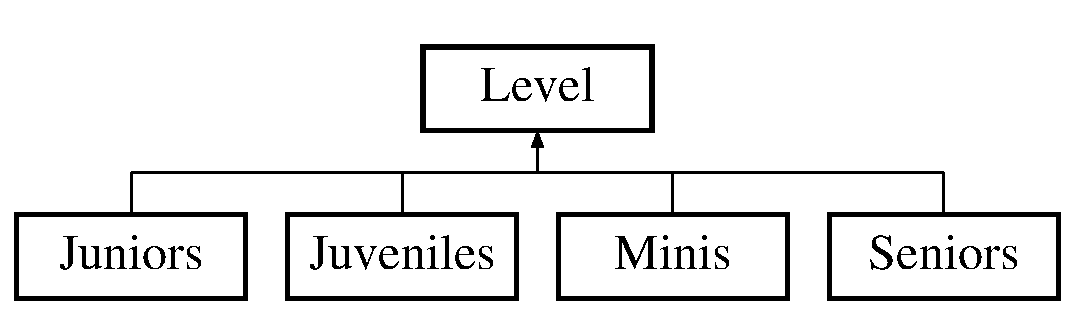
\includegraphics[height=2.000000cm]{class_level}
\end{center}
\end{figure}
\subsection*{Public Member Functions}
\begin{DoxyCompactItemize}
\item 
\hyperlink{class_level_a7a696c928ca5d5354db6e50e46d0f67d}{Level} ()
\begin{DoxyCompactList}\small\item\em Default constructor. \end{DoxyCompactList}\item 
virtual \hyperlink{class_level_a249eac1e8f19ff44134efa5e986feaca}{$\sim$\+Level} ()
\begin{DoxyCompactList}\small\item\em Destructor. \end{DoxyCompactList}\item 
\hyperlink{class_level_a098e3e980b18013bf7f0683acbe5e2f6}{Level} (const \hyperlink{class_level}{Level} \&level)
\begin{DoxyCompactList}\small\item\em Copy constructor. \end{DoxyCompactList}\item 
\hyperlink{class_level}{Level} \& \hyperlink{class_level_a60eb04b65c900ae8dddf3d6251fac7b1}{operator=} (const \hyperlink{class_level}{Level} \&level)
\begin{DoxyCompactList}\small\item\em Copy Operator. \end{DoxyCompactList}\item 
virtual unsigned int \hyperlink{class_level_ae7b28ba0cb8d49372c4657fbe42706e1}{get\+Max\+Age} ()=0
\begin{DoxyCompactList}\small\item\em Get the maximum age to be on this \hyperlink{class_level}{Level}. \end{DoxyCompactList}\item 
virtual unsigned int \hyperlink{class_level_a161cf8c238fd499c112d90504cb6f587}{get\+Min\+Age} ()=0
\begin{DoxyCompactList}\small\item\em Get the minimum age to be on this \hyperlink{class_level}{Level}. \end{DoxyCompactList}\item 
vector$<$ \hyperlink{class_player}{Player} $\ast$ $>$ \hyperlink{class_level_a51ff82259c62111618aed20f96ec9f88}{get\+Players} () const
\begin{DoxyCompactList}\small\item\em Gets all of the Players on this \hyperlink{class_level}{Level}. \end{DoxyCompactList}\item 
vector$<$ \hyperlink{class_event}{Event} $\ast$ $>$ \hyperlink{class_level_aa03432096cfcf42293cebf2c801b7437}{get\+Events} () const
\begin{DoxyCompactList}\small\item\em Gets all of the Events on this \hyperlink{class_level}{Level}. \end{DoxyCompactList}\item 
string \hyperlink{class_level_a6c4d3f153c3285aeaf3ec954981c5be8}{get\+Coach} () const
\begin{DoxyCompactList}\small\item\em Gets the coach of this \hyperlink{class_level}{Level}. \end{DoxyCompactList}\item 
\hyperlink{class_b_s_t}{B\+ST}$<$ \hyperlink{struct_player__node}{Player\+\_\+node} $>$ \hyperlink{class_level_ae24a0ba5c352e1cb0fa64282a89e559f}{get\+Players\+\_\+tree} () const
\begin{DoxyCompactList}\small\item\em Gets the \hyperlink{class_b_s_t}{B\+ST} of players on this \hyperlink{class_level}{Level}. \end{DoxyCompactList}\item 
vector$<$ \hyperlink{class_event}{Event} $\ast$ $>$ \hyperlink{class_level_a58a416953fdf79d4b6388cd6bd0b4e95}{get\+Trainings} () const
\begin{DoxyCompactList}\small\item\em Gets all of the Trainings of this \hyperlink{class_level}{Level}. \end{DoxyCompactList}\item 
vector$<$ \hyperlink{class_event}{Event} $\ast$ $>$ \hyperlink{class_level_a20beb75d82f194ad901e6193ee728d81}{get\+Tournaments} () const
\begin{DoxyCompactList}\small\item\em Gets all of the Tournaments of this \hyperlink{class_level}{Level}. \end{DoxyCompactList}\item 
virtual bool \hyperlink{class_level_a66290778fa4bcd2f29b9ff3e605b2902}{add\+Player} (\hyperlink{class_player}{Player} $\ast$player)
\begin{DoxyCompactList}\small\item\em Adds a new \hyperlink{class_player}{Player} to this \hyperlink{class_level}{Level}. \end{DoxyCompactList}\item 
void \hyperlink{class_level_a86b0d3ec7bb14fd7002c332b328dd96d}{add\+Event} (\hyperlink{class_event}{Event} $\ast$event)
\begin{DoxyCompactList}\small\item\em Adds a new \hyperlink{class_event}{Event} to this \hyperlink{class_level}{Level}. \end{DoxyCompactList}\item 
void \hyperlink{class_level_aa666e5fe87af336fd7350ac0b72b7c8c}{set\+Coach} (std\+::string coach)
\begin{DoxyCompactList}\small\item\em Changes coach name. \end{DoxyCompactList}\item 
virtual void \hyperlink{class_level_a40d22b376e72950a07de5e0a9e288029}{showplayers} () const
\begin{DoxyCompactList}\small\item\em Outputs the Players of this \hyperlink{class_level}{Level} to the screen. \end{DoxyCompactList}\item 
virtual void \hyperlink{class_level_a4101cb725b1fd0c0836834c92b190363}{showtrainings} () const
\begin{DoxyCompactList}\small\item\em Outputs the Trainings of this \hyperlink{class_level}{Level} to the screen. \end{DoxyCompactList}\item 
virtual void \hyperlink{class_level_a757c4547f3b8f7c7ecb02c7e0e6cd7c9}{showtournaments} () const
\begin{DoxyCompactList}\small\item\em Outputs the Tournaments of this \hyperlink{class_level}{Level} to the screen. \end{DoxyCompactList}\item 
virtual void \hyperlink{class_level_a8115b8f2e69ce1fdc21c64525c61a957}{showevents} () const
\begin{DoxyCompactList}\small\item\em Outputs the next events to happen. \end{DoxyCompactList}\item 
void \hyperlink{class_level_a68ca29bc1f8796b8ee89f6d9a77b3e2a}{removeplayer} (unsigned int id)
\begin{DoxyCompactList}\small\item\em Removes a \hyperlink{class_player}{Player} from this \hyperlink{class_level}{Level}. \end{DoxyCompactList}\item 
void \hyperlink{class_level_a8f38f4c5bc05c7c7c4d4ea1321d91b84}{remove\+Event} (unsigned int id)
\begin{DoxyCompactList}\small\item\em Removes an \hyperlink{class_event}{Event} from this \hyperlink{class_level}{Level}. \end{DoxyCompactList}\item 
vector$<$ \hyperlink{class_event}{Event} $\ast$ $>$ \hyperlink{class_level_a2c4cb023c042409bd7551a91f369a990}{get\+Future\+Events} ()
\begin{DoxyCompactList}\small\item\em Gets Events that will happen in the future. \end{DoxyCompactList}\item 
void \hyperlink{class_level_ac7ecbf06c831f2a02cad567bcfb52ec9}{raiseassiduity} (vector$<$ string $>$ players)
\begin{DoxyCompactList}\small\item\em Raises the assiduity of the Players. \end{DoxyCompactList}\item 
void \hyperlink{class_level_ab4e4b8c386063fd8244042f7eefa3427}{lowerassiduity} (vector$<$ string $>$ players)
\begin{DoxyCompactList}\small\item\em Lowers the assiduity of the Players. \end{DoxyCompactList}\item 
void \hyperlink{class_level_a2d64a6f446a4d6c7c4959c7bc0972a84}{raisepgames} (vector$<$ string $>$ players)
\begin{DoxyCompactList}\small\item\em Raises the presences in games of the Players. \end{DoxyCompactList}\item 
void \hyperlink{class_level_a336a54c2ef7e4307e9353a200a11537e}{lowerpgames} (vector$<$ string $>$ players)
\begin{DoxyCompactList}\small\item\em Lowers the presences in games of the Players. \end{DoxyCompactList}\item 
void \hyperlink{class_level_ac592cc97524f49de9114f4af20312aad}{raiseptournaments} (vector$<$ string $>$ players)
\begin{DoxyCompactList}\small\item\em Raises the presences in tournaments of the Players. \end{DoxyCompactList}\item 
void \hyperlink{class_level_afbb999a489e4e185bb26e965939a97e5}{lowerptournaments} (vector$<$ string $>$ players)
\begin{DoxyCompactList}\small\item\em Lowers the presences in tournaments of the Players. \end{DoxyCompactList}\item 
void \hyperlink{class_level_af91bf73255a171a3f2a256778e075fb7}{raisegames\+\_\+won} (vector$<$ string $>$ players, int value, vector$<$ pair$<$ pair$<$ unsigned int, unsigned int $>$, string $>$$>$ results)
\begin{DoxyCompactList}\small\item\em Raises the number of games in which this \hyperlink{class_level}{Level} won that the Players participated. \end{DoxyCompactList}\item 
void \hyperlink{class_level_a2634c6743f1a56592c97e6cfb7a9a8b6}{raiseassiduity\+\_\+curr} (vector$<$ string $>$ player, int value)
\begin{DoxyCompactList}\small\item\em Increases the value of assiduity of Players. \end{DoxyCompactList}\item 
virtual vector$<$ string $>$ \hyperlink{class_level_ac118b390f16a75b9a0e9df198b3190ad}{get\+Call} (unsigned int size)=0
\begin{DoxyCompactList}\small\item\em Makes a call for an \hyperlink{class_event}{Event}. \end{DoxyCompactList}\item 
void \hyperlink{class_level_a09a28b62e9b593db54b220533a5dd567}{actualize\+\_\+curr\+\_\+parameters} ()
\begin{DoxyCompactList}\small\item\em Re-\/computes the assiduities of all the Players in this \hyperlink{class_level}{Level}. \end{DoxyCompactList}\item 
void \hyperlink{class_level_a45217bde102ee160f4852d093f51ed83}{make\+Tree} ()
\begin{DoxyCompactList}\small\item\em Constructs the member variable players\+\_\+tree with the current Players. \end{DoxyCompactList}\item 
void \hyperlink{class_level_a2752e4f84d3de5e8b72e4cf87cb0131b}{remove\+\_\+\+Tree} (\hyperlink{struct_player__node}{Player\+\_\+node} pl)
\begin{DoxyCompactList}\small\item\em Removes a \hyperlink{class_player}{Player} from the member variable players\+\_\+tree. \end{DoxyCompactList}\end{DoxyCompactItemize}


\subsection{Detailed Description}
Holds all the information about the \hyperlink{class_club}{Club}. 

Definition at line 36 of file Level.\+h.



\subsection{Constructor \& Destructor Documentation}
\hypertarget{class_level_a7a696c928ca5d5354db6e50e46d0f67d}{}\label{class_level_a7a696c928ca5d5354db6e50e46d0f67d} 
\index{Level@{Level}!Level@{Level}}
\index{Level@{Level}!Level@{Level}}
\subsubsection{\texorpdfstring{Level()}{Level()}\hspace{0.1cm}{\footnotesize\ttfamily [1/2]}}
{\footnotesize\ttfamily Level\+::\+Level (\begin{DoxyParamCaption}{ }\end{DoxyParamCaption})\hspace{0.3cm}{\ttfamily [inline]}}



Default constructor. 

Initializes the \hyperlink{class_b_s_t}{B\+ST} 

Definition at line 46 of file Level.\+h.

\hypertarget{class_level_a249eac1e8f19ff44134efa5e986feaca}{}\label{class_level_a249eac1e8f19ff44134efa5e986feaca} 
\index{Level@{Level}!````~Level@{$\sim$\+Level}}
\index{````~Level@{$\sim$\+Level}!Level@{Level}}
\subsubsection{\texorpdfstring{$\sim$\+Level()}{~Level()}}
{\footnotesize\ttfamily Level\+::$\sim$\+Level (\begin{DoxyParamCaption}{ }\end{DoxyParamCaption})\hspace{0.3cm}{\ttfamily [virtual]}}



Destructor. 



Definition at line 8 of file Level.\+cpp.

\hypertarget{class_level_a098e3e980b18013bf7f0683acbe5e2f6}{}\label{class_level_a098e3e980b18013bf7f0683acbe5e2f6} 
\index{Level@{Level}!Level@{Level}}
\index{Level@{Level}!Level@{Level}}
\subsubsection{\texorpdfstring{Level()}{Level()}\hspace{0.1cm}{\footnotesize\ttfamily [2/2]}}
{\footnotesize\ttfamily Level\+::\+Level (\begin{DoxyParamCaption}\item[{const \hyperlink{class_level}{Level} \&}]{level }\end{DoxyParamCaption})}



Copy constructor. 


\begin{DoxyParams}{Parameters}
{\em level} & Object of \hyperlink{class_level}{Level} to be copied \\
\hline
\end{DoxyParams}


Definition at line 20 of file Level.\+cpp.



\subsection{Member Function Documentation}
\hypertarget{class_level_a09a28b62e9b593db54b220533a5dd567}{}\label{class_level_a09a28b62e9b593db54b220533a5dd567} 
\index{Level@{Level}!actualize\+\_\+curr\+\_\+parameters@{actualize\+\_\+curr\+\_\+parameters}}
\index{actualize\+\_\+curr\+\_\+parameters@{actualize\+\_\+curr\+\_\+parameters}!Level@{Level}}
\subsubsection{\texorpdfstring{actualize\+\_\+curr\+\_\+parameters()}{actualize\_curr\_parameters()}}
{\footnotesize\ttfamily void Level\+::actualize\+\_\+curr\+\_\+parameters (\begin{DoxyParamCaption}{ }\end{DoxyParamCaption})}



Re-\/computes the assiduities of all the Players in this \hyperlink{class_level}{Level}. 



Definition at line 338 of file Level.\+cpp.

\hypertarget{class_level_a86b0d3ec7bb14fd7002c332b328dd96d}{}\label{class_level_a86b0d3ec7bb14fd7002c332b328dd96d} 
\index{Level@{Level}!add\+Event@{add\+Event}}
\index{add\+Event@{add\+Event}!Level@{Level}}
\subsubsection{\texorpdfstring{add\+Event()}{addEvent()}}
{\footnotesize\ttfamily void Level\+::add\+Event (\begin{DoxyParamCaption}\item[{\hyperlink{class_event}{Event} $\ast$}]{event }\end{DoxyParamCaption})}



Adds a new \hyperlink{class_event}{Event} to this \hyperlink{class_level}{Level}. 


\begin{DoxyParams}{Parameters}
{\em event} & New \hyperlink{class_event}{Event} to be added \\
\hline
\end{DoxyParams}


Definition at line 103 of file Level.\+cpp.

\hypertarget{class_level_a66290778fa4bcd2f29b9ff3e605b2902}{}\label{class_level_a66290778fa4bcd2f29b9ff3e605b2902} 
\index{Level@{Level}!add\+Player@{add\+Player}}
\index{add\+Player@{add\+Player}!Level@{Level}}
\subsubsection{\texorpdfstring{add\+Player()}{addPlayer()}}
{\footnotesize\ttfamily bool Level\+::add\+Player (\begin{DoxyParamCaption}\item[{\hyperlink{class_player}{Player} $\ast$}]{player }\end{DoxyParamCaption})\hspace{0.3cm}{\ttfamily [virtual]}}



Adds a new \hyperlink{class_player}{Player} to this \hyperlink{class_level}{Level}. 


\begin{DoxyParams}{Parameters}
{\em player} & New \hyperlink{class_player}{Player} to be added \\
\hline
\end{DoxyParams}
\begin{DoxyReturn}{Returns}
True if the \hyperlink{class_player}{Player} was inserted successfuly, false if not
\end{DoxyReturn}
The \hyperlink{class_player}{Player} can not be added to the \hyperlink{class_level}{Level} if his age is not within the range of admitted ages 

Reimplemented in \hyperlink{class_juniors_a23915dab5b0c30a978f08a653483db53}{Juniors}, \hyperlink{class_seniors_a4ee5683212625ee909b5c04d08bc8823}{Seniors}, \hyperlink{class_juveniles_a596c6380325142d8c49c8d8db7b9fa31}{Juveniles}, and \hyperlink{class_minis_a75f45698aaf057d11e083694bfd31d17}{Minis}.



Definition at line 85 of file Level.\+cpp.

\hypertarget{class_level_ac118b390f16a75b9a0e9df198b3190ad}{}\label{class_level_ac118b390f16a75b9a0e9df198b3190ad} 
\index{Level@{Level}!get\+Call@{get\+Call}}
\index{get\+Call@{get\+Call}!Level@{Level}}
\subsubsection{\texorpdfstring{get\+Call()}{getCall()}}
{\footnotesize\ttfamily virtual vector$<$string$>$ Level\+::get\+Call (\begin{DoxyParamCaption}\item[{unsigned int}]{size }\end{DoxyParamCaption})\hspace{0.3cm}{\ttfamily [pure virtual]}}



Makes a call for an \hyperlink{class_event}{Event}. 


\begin{DoxyParams}{Parameters}
{\em size} & How many Players to call \\
\hline
\end{DoxyParams}
\begin{DoxyReturn}{Returns}
Vector with the players called to the \hyperlink{class_event}{Event}
\end{DoxyReturn}
Pure Virtual, to be implemented by derived classes 

Implemented in \hyperlink{class_juniors_ace1da8267f2a92dbfb9e27f7b6b95d26}{Juniors}, \hyperlink{class_seniors_a3b2fbe1e5d735c7659a195cea6333a0b}{Seniors}, \hyperlink{class_juveniles_a062cff0b64c844c3e9cc9b41e768cce6}{Juveniles}, and \hyperlink{class_minis_ad2c86c585b05e735bb6e38f672b9bbab}{Minis}.

\hypertarget{class_level_a6c4d3f153c3285aeaf3ec954981c5be8}{}\label{class_level_a6c4d3f153c3285aeaf3ec954981c5be8} 
\index{Level@{Level}!get\+Coach@{get\+Coach}}
\index{get\+Coach@{get\+Coach}!Level@{Level}}
\subsubsection{\texorpdfstring{get\+Coach()}{getCoach()}}
{\footnotesize\ttfamily string Level\+::get\+Coach (\begin{DoxyParamCaption}{ }\end{DoxyParamCaption}) const\hspace{0.3cm}{\ttfamily [inline]}}



Gets the coach of this \hyperlink{class_level}{Level}. 

\begin{DoxyReturn}{Returns}
coach (member variable) 
\end{DoxyReturn}


Definition at line 85 of file Level.\+h.

\hypertarget{class_level_aa03432096cfcf42293cebf2c801b7437}{}\label{class_level_aa03432096cfcf42293cebf2c801b7437} 
\index{Level@{Level}!get\+Events@{get\+Events}}
\index{get\+Events@{get\+Events}!Level@{Level}}
\subsubsection{\texorpdfstring{get\+Events()}{getEvents()}}
{\footnotesize\ttfamily vector$<$\hyperlink{class_event}{Event} $\ast$$>$ Level\+::get\+Events (\begin{DoxyParamCaption}{ }\end{DoxyParamCaption}) const\hspace{0.3cm}{\ttfamily [inline]}}



Gets all of the Events on this \hyperlink{class_level}{Level}. 

\begin{DoxyReturn}{Returns}
events (member variable) 
\end{DoxyReturn}


Definition at line 80 of file Level.\+h.

\hypertarget{class_level_a2c4cb023c042409bd7551a91f369a990}{}\label{class_level_a2c4cb023c042409bd7551a91f369a990} 
\index{Level@{Level}!get\+Future\+Events@{get\+Future\+Events}}
\index{get\+Future\+Events@{get\+Future\+Events}!Level@{Level}}
\subsubsection{\texorpdfstring{get\+Future\+Events()}{getFutureEvents()}}
{\footnotesize\ttfamily vector$<$ \hyperlink{class_event}{Event} $\ast$ $>$ Level\+::get\+Future\+Events (\begin{DoxyParamCaption}{ }\end{DoxyParamCaption})}



Gets Events that will happen in the future. 

\begin{DoxyReturn}{Returns}
Vector of the Events to happen 
\end{DoxyReturn}


Definition at line 217 of file Level.\+cpp.

\hypertarget{class_level_ae7b28ba0cb8d49372c4657fbe42706e1}{}\label{class_level_ae7b28ba0cb8d49372c4657fbe42706e1} 
\index{Level@{Level}!get\+Max\+Age@{get\+Max\+Age}}
\index{get\+Max\+Age@{get\+Max\+Age}!Level@{Level}}
\subsubsection{\texorpdfstring{get\+Max\+Age()}{getMaxAge()}}
{\footnotesize\ttfamily virtual unsigned int Level\+::get\+Max\+Age (\begin{DoxyParamCaption}{ }\end{DoxyParamCaption})\hspace{0.3cm}{\ttfamily [pure virtual]}}



Get the maximum age to be on this \hyperlink{class_level}{Level}. 

Pure Virtual, to be inherited by derived classes 

Implemented in \hyperlink{class_juniors_a98c28047a2d5ff2b14651ee9eccfd2b6}{Juniors}, \hyperlink{class_seniors_a856a5d37a9dbda1e1b3ad8eb90db1f2a}{Seniors}, \hyperlink{class_juveniles_a6b7825beb91d790fc5432902aedcc1fc}{Juveniles}, and \hyperlink{class_minis_a995e2db860e3a5c110cbead80ab61caa}{Minis}.

\hypertarget{class_level_a161cf8c238fd499c112d90504cb6f587}{}\label{class_level_a161cf8c238fd499c112d90504cb6f587} 
\index{Level@{Level}!get\+Min\+Age@{get\+Min\+Age}}
\index{get\+Min\+Age@{get\+Min\+Age}!Level@{Level}}
\subsubsection{\texorpdfstring{get\+Min\+Age()}{getMinAge()}}
{\footnotesize\ttfamily virtual unsigned int Level\+::get\+Min\+Age (\begin{DoxyParamCaption}{ }\end{DoxyParamCaption})\hspace{0.3cm}{\ttfamily [pure virtual]}}



Get the minimum age to be on this \hyperlink{class_level}{Level}. 

Pure Virtual, to be inherited by derived classes 

Implemented in \hyperlink{class_juniors_a3110bdbaa344b2bfefa2ddcb8be8d7c6}{Juniors}, \hyperlink{class_seniors_a1843edaf8811f4728f76c11c79fe5450}{Seniors}, \hyperlink{class_juveniles_a033b591527e3398a05da40e5ab954b40}{Juveniles}, and \hyperlink{class_minis_a062e99b463e0dd1e370b46e6fb37087a}{Minis}.

\hypertarget{class_level_a51ff82259c62111618aed20f96ec9f88}{}\label{class_level_a51ff82259c62111618aed20f96ec9f88} 
\index{Level@{Level}!get\+Players@{get\+Players}}
\index{get\+Players@{get\+Players}!Level@{Level}}
\subsubsection{\texorpdfstring{get\+Players()}{getPlayers()}}
{\footnotesize\ttfamily vector$<$\hyperlink{class_player}{Player} $\ast$$>$ Level\+::get\+Players (\begin{DoxyParamCaption}{ }\end{DoxyParamCaption}) const\hspace{0.3cm}{\ttfamily [inline]}}



Gets all of the Players on this \hyperlink{class_level}{Level}. 

\begin{DoxyReturn}{Returns}
players (member variable) 
\end{DoxyReturn}


Definition at line 75 of file Level.\+h.

\hypertarget{class_level_ae24a0ba5c352e1cb0fa64282a89e559f}{}\label{class_level_ae24a0ba5c352e1cb0fa64282a89e559f} 
\index{Level@{Level}!get\+Players\+\_\+tree@{get\+Players\+\_\+tree}}
\index{get\+Players\+\_\+tree@{get\+Players\+\_\+tree}!Level@{Level}}
\subsubsection{\texorpdfstring{get\+Players\+\_\+tree()}{getPlayers\_tree()}}
{\footnotesize\ttfamily \hyperlink{class_b_s_t}{B\+ST}$<$\hyperlink{struct_player__node}{Player\+\_\+node}$>$ Level\+::get\+Players\+\_\+tree (\begin{DoxyParamCaption}{ }\end{DoxyParamCaption}) const\hspace{0.3cm}{\ttfamily [inline]}}



Gets the \hyperlink{class_b_s_t}{B\+ST} of players on this \hyperlink{class_level}{Level}. 

\begin{DoxyReturn}{Returns}
players\+\_\+tree (member variable) 
\end{DoxyReturn}


Definition at line 90 of file Level.\+h.

\hypertarget{class_level_a20beb75d82f194ad901e6193ee728d81}{}\label{class_level_a20beb75d82f194ad901e6193ee728d81} 
\index{Level@{Level}!get\+Tournaments@{get\+Tournaments}}
\index{get\+Tournaments@{get\+Tournaments}!Level@{Level}}
\subsubsection{\texorpdfstring{get\+Tournaments()}{getTournaments()}}
{\footnotesize\ttfamily vector$<$ \hyperlink{class_event}{Event} $\ast$ $>$ Level\+::get\+Tournaments (\begin{DoxyParamCaption}{ }\end{DoxyParamCaption}) const}



Gets all of the Tournaments of this \hyperlink{class_level}{Level}. 

\begin{DoxyReturn}{Returns}
Vector only with Tournaments 
\end{DoxyReturn}


Definition at line 69 of file Level.\+cpp.

\hypertarget{class_level_a58a416953fdf79d4b6388cd6bd0b4e95}{}\label{class_level_a58a416953fdf79d4b6388cd6bd0b4e95} 
\index{Level@{Level}!get\+Trainings@{get\+Trainings}}
\index{get\+Trainings@{get\+Trainings}!Level@{Level}}
\subsubsection{\texorpdfstring{get\+Trainings()}{getTrainings()}}
{\footnotesize\ttfamily vector$<$ \hyperlink{class_event}{Event} $\ast$ $>$ Level\+::get\+Trainings (\begin{DoxyParamCaption}{ }\end{DoxyParamCaption}) const}



Gets all of the Trainings of this \hyperlink{class_level}{Level}. 

\begin{DoxyReturn}{Returns}
Vector only with Trainings 
\end{DoxyReturn}


Definition at line 56 of file Level.\+cpp.

\hypertarget{class_level_ab4e4b8c386063fd8244042f7eefa3427}{}\label{class_level_ab4e4b8c386063fd8244042f7eefa3427} 
\index{Level@{Level}!lowerassiduity@{lowerassiduity}}
\index{lowerassiduity@{lowerassiduity}!Level@{Level}}
\subsubsection{\texorpdfstring{lowerassiduity()}{lowerassiduity()}}
{\footnotesize\ttfamily void Level\+::lowerassiduity (\begin{DoxyParamCaption}\item[{vector$<$ string $>$}]{players }\end{DoxyParamCaption})}



Lowers the assiduity of the Players. 


\begin{DoxyParams}{Parameters}
{\em players} & Vector of players to lower the assiduity (member varible in \hyperlink{class_player}{Player}) \\
\hline
\end{DoxyParams}


Definition at line 244 of file Level.\+cpp.

\hypertarget{class_level_a336a54c2ef7e4307e9353a200a11537e}{}\label{class_level_a336a54c2ef7e4307e9353a200a11537e} 
\index{Level@{Level}!lowerpgames@{lowerpgames}}
\index{lowerpgames@{lowerpgames}!Level@{Level}}
\subsubsection{\texorpdfstring{lowerpgames()}{lowerpgames()}}
{\footnotesize\ttfamily void Level\+::lowerpgames (\begin{DoxyParamCaption}\item[{vector$<$ string $>$}]{players }\end{DoxyParamCaption})}



Lowers the presences in games of the Players. 


\begin{DoxyParams}{Parameters}
{\em players} & Vector of players to lower the pgames (member varible in \hyperlink{class_player}{Player}) \\
\hline
\end{DoxyParams}


Definition at line 269 of file Level.\+cpp.

\hypertarget{class_level_afbb999a489e4e185bb26e965939a97e5}{}\label{class_level_afbb999a489e4e185bb26e965939a97e5} 
\index{Level@{Level}!lowerptournaments@{lowerptournaments}}
\index{lowerptournaments@{lowerptournaments}!Level@{Level}}
\subsubsection{\texorpdfstring{lowerptournaments()}{lowerptournaments()}}
{\footnotesize\ttfamily void Level\+::lowerptournaments (\begin{DoxyParamCaption}\item[{vector$<$ string $>$}]{players }\end{DoxyParamCaption})}



Lowers the presences in tournaments of the Players. 


\begin{DoxyParams}{Parameters}
{\em players} & Vector of players to lower the ptournaments (member varible in \hyperlink{class_player}{Player}) \\
\hline
\end{DoxyParams}


Definition at line 293 of file Level.\+cpp.

\hypertarget{class_level_a45217bde102ee160f4852d093f51ed83}{}\label{class_level_a45217bde102ee160f4852d093f51ed83} 
\index{Level@{Level}!make\+Tree@{make\+Tree}}
\index{make\+Tree@{make\+Tree}!Level@{Level}}
\subsubsection{\texorpdfstring{make\+Tree()}{makeTree()}}
{\footnotesize\ttfamily void Level\+::make\+Tree (\begin{DoxyParamCaption}{ }\end{DoxyParamCaption})}



Constructs the member variable players\+\_\+tree with the current Players. 



Definition at line 359 of file Level.\+cpp.

\hypertarget{class_level_a60eb04b65c900ae8dddf3d6251fac7b1}{}\label{class_level_a60eb04b65c900ae8dddf3d6251fac7b1} 
\index{Level@{Level}!operator=@{operator=}}
\index{operator=@{operator=}!Level@{Level}}
\subsubsection{\texorpdfstring{operator=()}{operator=()}}
{\footnotesize\ttfamily \hyperlink{class_level}{Level} \& Level\+::operator= (\begin{DoxyParamCaption}\item[{const \hyperlink{class_level}{Level} \&}]{level }\end{DoxyParamCaption})}



Copy Operator. 


\begin{DoxyParams}{Parameters}
{\em level} & Object of \hyperlink{class_level}{Level} to be copied \\
\hline
\end{DoxyParams}


Definition at line 38 of file Level.\+cpp.

\hypertarget{class_level_ac7ecbf06c831f2a02cad567bcfb52ec9}{}\label{class_level_ac7ecbf06c831f2a02cad567bcfb52ec9} 
\index{Level@{Level}!raiseassiduity@{raiseassiduity}}
\index{raiseassiduity@{raiseassiduity}!Level@{Level}}
\subsubsection{\texorpdfstring{raiseassiduity()}{raiseassiduity()}}
{\footnotesize\ttfamily void Level\+::raiseassiduity (\begin{DoxyParamCaption}\item[{vector$<$ string $>$}]{players }\end{DoxyParamCaption})}



Raises the assiduity of the Players. 


\begin{DoxyParams}{Parameters}
{\em players} & Vector of players to raise the assiduity (member varible in \hyperlink{class_player}{Player}) \\
\hline
\end{DoxyParams}


Definition at line 232 of file Level.\+cpp.

\hypertarget{class_level_a2634c6743f1a56592c97e6cfb7a9a8b6}{}\label{class_level_a2634c6743f1a56592c97e6cfb7a9a8b6} 
\index{Level@{Level}!raiseassiduity\+\_\+curr@{raiseassiduity\+\_\+curr}}
\index{raiseassiduity\+\_\+curr@{raiseassiduity\+\_\+curr}!Level@{Level}}
\subsubsection{\texorpdfstring{raiseassiduity\+\_\+curr()}{raiseassiduity\_curr()}}
{\footnotesize\ttfamily void Level\+::raiseassiduity\+\_\+curr (\begin{DoxyParamCaption}\item[{vector$<$ string $>$}]{player,  }\item[{int}]{value }\end{DoxyParamCaption})}



Increases the value of assiduity of Players. 


\begin{DoxyParams}{Parameters}
{\em player} & Vector of names of \hyperlink{class_player}{Player} to be increased \\
\hline
{\em value} & Number of points to be increased \\
\hline
\end{DoxyParams}


Definition at line 326 of file Level.\+cpp.

\hypertarget{class_level_af91bf73255a171a3f2a256778e075fb7}{}\label{class_level_af91bf73255a171a3f2a256778e075fb7} 
\index{Level@{Level}!raisegames\+\_\+won@{raisegames\+\_\+won}}
\index{raisegames\+\_\+won@{raisegames\+\_\+won}!Level@{Level}}
\subsubsection{\texorpdfstring{raisegames\+\_\+won()}{raisegames\_won()}}
{\footnotesize\ttfamily void Level\+::raisegames\+\_\+won (\begin{DoxyParamCaption}\item[{vector$<$ string $>$}]{players,  }\item[{int}]{value,  }\item[{vector$<$ pair$<$ pair$<$ unsigned int, unsigned int $>$, string $>$$>$}]{results }\end{DoxyParamCaption})}



Raises the number of games in which this \hyperlink{class_level}{Level} won that the Players participated. 


\begin{DoxyParams}{Parameters}
{\em players} & Players to be raised \\
\hline
{\em value} & Amount to be raised \\
\hline
{\em results} & Results achieved by the \hyperlink{class_level}{Level}\\
\hline
\end{DoxyParams}
Computes how many games where won from the parameter results then multiplies it by value and adds to each player 

Definition at line 307 of file Level.\+cpp.

\hypertarget{class_level_a2d64a6f446a4d6c7c4959c7bc0972a84}{}\label{class_level_a2d64a6f446a4d6c7c4959c7bc0972a84} 
\index{Level@{Level}!raisepgames@{raisepgames}}
\index{raisepgames@{raisepgames}!Level@{Level}}
\subsubsection{\texorpdfstring{raisepgames()}{raisepgames()}}
{\footnotesize\ttfamily void Level\+::raisepgames (\begin{DoxyParamCaption}\item[{vector$<$ string $>$}]{players }\end{DoxyParamCaption})}



Raises the presences in games of the Players. 


\begin{DoxyParams}{Parameters}
{\em players} & Vector of players to raise the pgames (member variable in \hyperlink{class_player}{Player}) \\
\hline
\end{DoxyParams}


Definition at line 257 of file Level.\+cpp.

\hypertarget{class_level_ac592cc97524f49de9114f4af20312aad}{}\label{class_level_ac592cc97524f49de9114f4af20312aad} 
\index{Level@{Level}!raiseptournaments@{raiseptournaments}}
\index{raiseptournaments@{raiseptournaments}!Level@{Level}}
\subsubsection{\texorpdfstring{raiseptournaments()}{raiseptournaments()}}
{\footnotesize\ttfamily void Level\+::raiseptournaments (\begin{DoxyParamCaption}\item[{vector$<$ string $>$}]{players }\end{DoxyParamCaption})}



Raises the presences in tournaments of the Players. 


\begin{DoxyParams}{Parameters}
{\em players} & Vector of players to raise the ptournaments (member variable in \hyperlink{class_player}{Player}) \\
\hline
\end{DoxyParams}


Definition at line 281 of file Level.\+cpp.

\hypertarget{class_level_a2752e4f84d3de5e8b72e4cf87cb0131b}{}\label{class_level_a2752e4f84d3de5e8b72e4cf87cb0131b} 
\index{Level@{Level}!remove\+\_\+\+Tree@{remove\+\_\+\+Tree}}
\index{remove\+\_\+\+Tree@{remove\+\_\+\+Tree}!Level@{Level}}
\subsubsection{\texorpdfstring{remove\+\_\+\+Tree()}{remove\_Tree()}}
{\footnotesize\ttfamily void Level\+::remove\+\_\+\+Tree (\begin{DoxyParamCaption}\item[{\hyperlink{struct_player__node}{Player\+\_\+node}}]{pl }\end{DoxyParamCaption})\hspace{0.3cm}{\ttfamily [inline]}}



Removes a \hyperlink{class_player}{Player} from the member variable players\+\_\+tree. 


\begin{DoxyParams}{Parameters}
{\em pl} & \hyperlink{class_player}{Player} to be removed from players\+\_\+tree \\
\hline
\end{DoxyParams}


Definition at line 216 of file Level.\+h.

\hypertarget{class_level_a8f38f4c5bc05c7c7c4d4ea1321d91b84}{}\label{class_level_a8f38f4c5bc05c7c7c4d4ea1321d91b84} 
\index{Level@{Level}!remove\+Event@{remove\+Event}}
\index{remove\+Event@{remove\+Event}!Level@{Level}}
\subsubsection{\texorpdfstring{remove\+Event()}{removeEvent()}}
{\footnotesize\ttfamily void Level\+::remove\+Event (\begin{DoxyParamCaption}\item[{unsigned int}]{id }\end{DoxyParamCaption})}



Removes an \hyperlink{class_event}{Event} from this \hyperlink{class_level}{Level}. 


\begin{DoxyParams}{Parameters}
{\em id} & Position in the member variable events \\
\hline
\end{DoxyParams}


Definition at line 210 of file Level.\+cpp.

\hypertarget{class_level_a68ca29bc1f8796b8ee89f6d9a77b3e2a}{}\label{class_level_a68ca29bc1f8796b8ee89f6d9a77b3e2a} 
\index{Level@{Level}!removeplayer@{removeplayer}}
\index{removeplayer@{removeplayer}!Level@{Level}}
\subsubsection{\texorpdfstring{removeplayer()}{removeplayer()}}
{\footnotesize\ttfamily void Level\+::removeplayer (\begin{DoxyParamCaption}\item[{unsigned int}]{id }\end{DoxyParamCaption})}



Removes a \hyperlink{class_player}{Player} from this \hyperlink{class_level}{Level}. 


\begin{DoxyParams}{Parameters}
{\em id} & Position in the member variable players \\
\hline
\end{DoxyParams}


Definition at line 197 of file Level.\+cpp.

\hypertarget{class_level_aa666e5fe87af336fd7350ac0b72b7c8c}{}\label{class_level_aa666e5fe87af336fd7350ac0b72b7c8c} 
\index{Level@{Level}!set\+Coach@{set\+Coach}}
\index{set\+Coach@{set\+Coach}!Level@{Level}}
\subsubsection{\texorpdfstring{set\+Coach()}{setCoach()}}
{\footnotesize\ttfamily void Level\+::set\+Coach (\begin{DoxyParamCaption}\item[{std\+::string}]{coach }\end{DoxyParamCaption})\hspace{0.3cm}{\ttfamily [inline]}}



Changes coach name. 


\begin{DoxyParams}{Parameters}
{\em coach} & Name of the coach \\
\hline
\end{DoxyParams}


Definition at line 117 of file Level.\+h.

\hypertarget{class_level_a8115b8f2e69ce1fdc21c64525c61a957}{}\label{class_level_a8115b8f2e69ce1fdc21c64525c61a957} 
\index{Level@{Level}!showevents@{showevents}}
\index{showevents@{showevents}!Level@{Level}}
\subsubsection{\texorpdfstring{showevents()}{showevents()}}
{\footnotesize\ttfamily void Level\+::showevents (\begin{DoxyParamCaption}{ }\end{DoxyParamCaption}) const\hspace{0.3cm}{\ttfamily [virtual]}}



Outputs the next events to happen. 

Includes both Trainings and Tournaments 

Definition at line 164 of file Level.\+cpp.

\hypertarget{class_level_a40d22b376e72950a07de5e0a9e288029}{}\label{class_level_a40d22b376e72950a07de5e0a9e288029} 
\index{Level@{Level}!showplayers@{showplayers}}
\index{showplayers@{showplayers}!Level@{Level}}
\subsubsection{\texorpdfstring{showplayers()}{showplayers()}}
{\footnotesize\ttfamily void Level\+::showplayers (\begin{DoxyParamCaption}{ }\end{DoxyParamCaption}) const\hspace{0.3cm}{\ttfamily [virtual]}}



Outputs the Players of this \hyperlink{class_level}{Level} to the screen. 

Pure Virtual, to be inherited by derived classes 

Reimplemented in \hyperlink{class_juniors_aa312c32ccc0c9d3193036c20849b8669}{Juniors}, \hyperlink{class_seniors_a671c22ddbb0c2df27adf12364db0380a}{Seniors}, \hyperlink{class_juveniles_ae66be24e5e17ce8583ff59c45ff4a772}{Juveniles}, and \hyperlink{class_minis_a062ba8858c80dcf52c792e5304ccbfeb}{Minis}.



Definition at line 116 of file Level.\+cpp.

\hypertarget{class_level_a757c4547f3b8f7c7ecb02c7e0e6cd7c9}{}\label{class_level_a757c4547f3b8f7c7ecb02c7e0e6cd7c9} 
\index{Level@{Level}!showtournaments@{showtournaments}}
\index{showtournaments@{showtournaments}!Level@{Level}}
\subsubsection{\texorpdfstring{showtournaments()}{showtournaments()}}
{\footnotesize\ttfamily void Level\+::showtournaments (\begin{DoxyParamCaption}{ }\end{DoxyParamCaption}) const\hspace{0.3cm}{\ttfamily [virtual]}}



Outputs the Tournaments of this \hyperlink{class_level}{Level} to the screen. 

Pure Virtual, to be inherited by derived classes 

Reimplemented in \hyperlink{class_juniors_a05afe7596b708ad635ac709499e66bc1}{Juniors}, \hyperlink{class_seniors_a5782adf80e1221220aa9e7bcaca5a3e3}{Seniors}, \hyperlink{class_juveniles_a8502c64d6a2cefda618003da25db3cda}{Juveniles}, and \hyperlink{class_minis_a1a8d585f0c4b745c9c703cc6449c778d}{Minis}.



Definition at line 146 of file Level.\+cpp.

\hypertarget{class_level_a4101cb725b1fd0c0836834c92b190363}{}\label{class_level_a4101cb725b1fd0c0836834c92b190363} 
\index{Level@{Level}!showtrainings@{showtrainings}}
\index{showtrainings@{showtrainings}!Level@{Level}}
\subsubsection{\texorpdfstring{showtrainings()}{showtrainings()}}
{\footnotesize\ttfamily void Level\+::showtrainings (\begin{DoxyParamCaption}{ }\end{DoxyParamCaption}) const\hspace{0.3cm}{\ttfamily [virtual]}}



Outputs the Trainings of this \hyperlink{class_level}{Level} to the screen. 

Pure Virtual, to be inherited by derived classes 

Reimplemented in \hyperlink{class_juniors_ad74d069390fffeda607de3584a0453de}{Juniors}, \hyperlink{class_seniors_a1f993a8ff143cc2e6dee8f3c81ed4cf3}{Seniors}, \hyperlink{class_juveniles_a168139683f59bca317a7d55cd33be5ac}{Juveniles}, and \hyperlink{class_minis_a69059ad5f89289c70ce6dec4906e02f3}{Minis}.



Definition at line 128 of file Level.\+cpp.



The documentation for this class was generated from the following files\+:\begin{DoxyCompactItemize}
\item 
/home/oco/\+Documents/\+Cprojects/\+Athletes/projecto -\/ V2/\+Headers/\hyperlink{_level_8h}{Level.\+h}\item 
/home/oco/\+Documents/\+Cprojects/\+Athletes/projecto -\/ V2/\+Source/\hyperlink{_level_8cpp}{Level.\+cpp}\end{DoxyCompactItemize}

\hypertarget{class_minis}{}\section{Minis Class Reference}
\label{class_minis}\index{Minis@{Minis}}


Holds all the information about the \hyperlink{class_level}{Level} \hyperlink{class_minis}{Minis}.  




{\ttfamily \#include $<$Minis.\+h$>$}

Inheritance diagram for Minis\+:\begin{figure}[H]
\begin{center}
\leavevmode
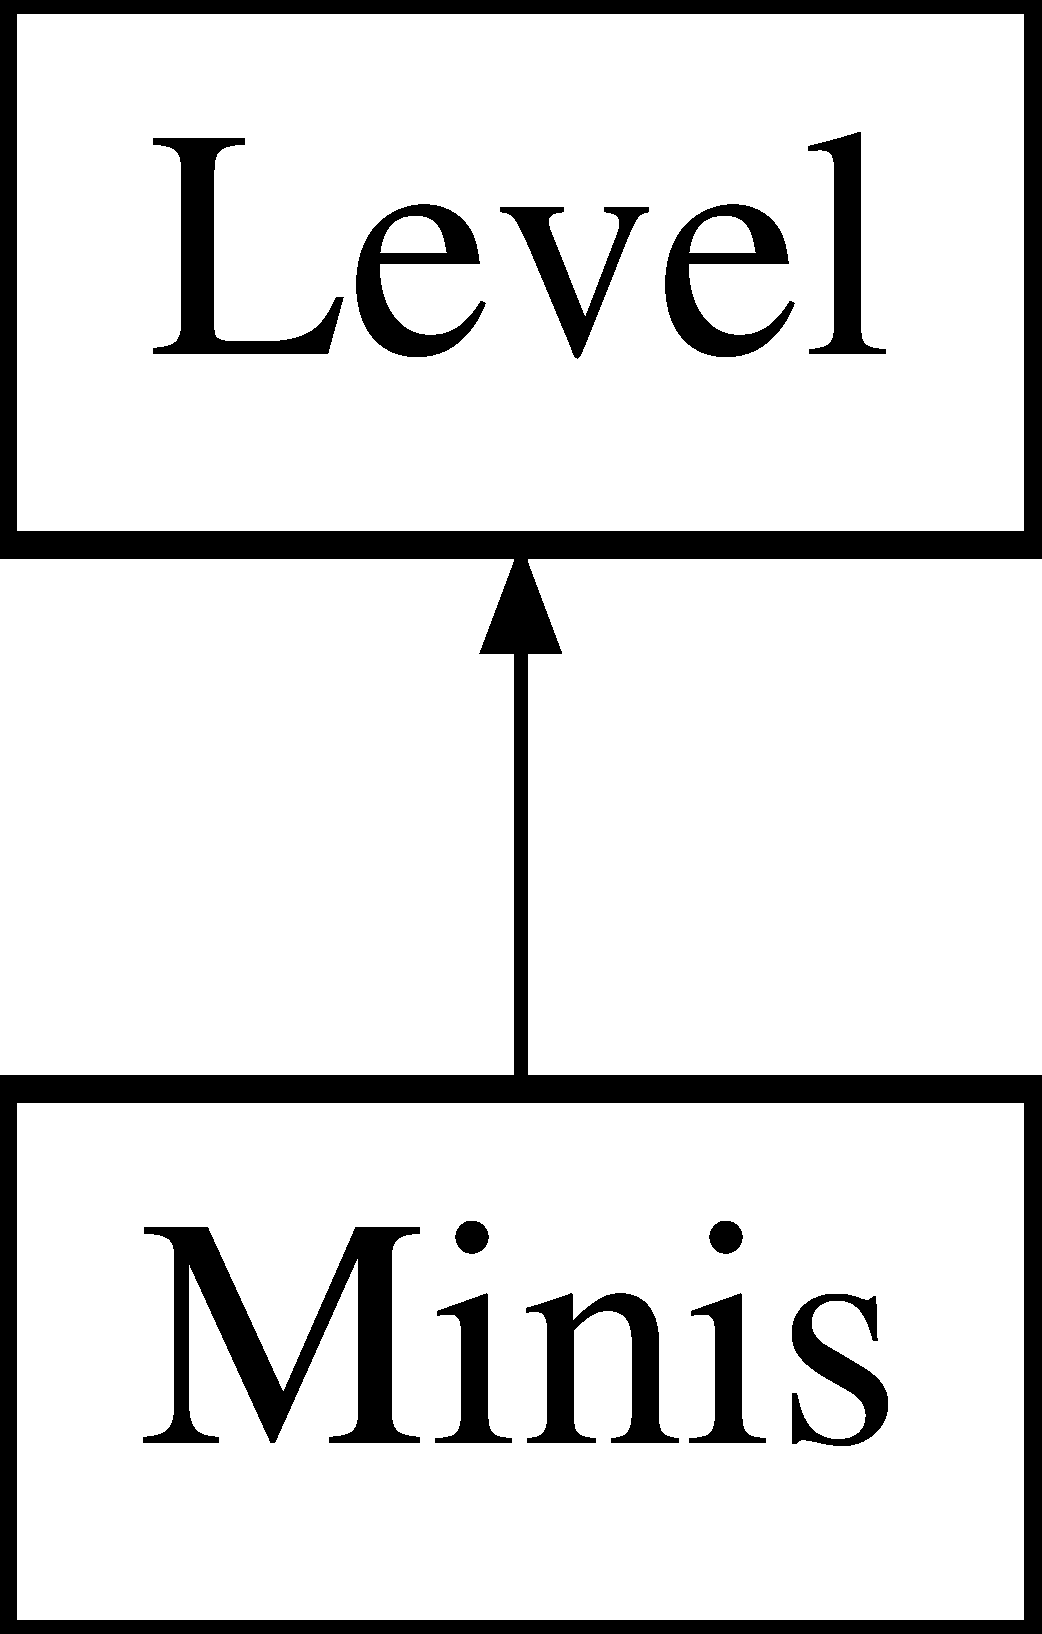
\includegraphics[height=2.000000cm]{class_minis}
\end{center}
\end{figure}
\subsection*{Public Member Functions}
\begin{DoxyCompactItemize}
\item 
\hyperlink{class_minis_a05a964e8cd328440070a970e95a69aaa}{Minis} ()
\begin{DoxyCompactList}\small\item\em Default Constructor. \end{DoxyCompactList}\item 
\hyperlink{class_minis_a0ce29fd41f5c3f412401128a9dc7dc3b}{$\sim$\+Minis} ()
\begin{DoxyCompactList}\small\item\em Destructor. \end{DoxyCompactList}\item 
\hyperlink{class_minis_a8f19940186bb60864cbf4b2a50a62f44}{Minis} (const \hyperlink{class_minis}{Minis} \&minis)
\begin{DoxyCompactList}\small\item\em Copy Constructor. \end{DoxyCompactList}\item 
\hyperlink{class_minis}{Minis} \& \hyperlink{class_minis_a25cdc8631f19c04d7ddd16507a4bc48c}{operator=} (const \hyperlink{class_minis}{Minis} \&minis)
\begin{DoxyCompactList}\small\item\em Copy Operator. \end{DoxyCompactList}\item 
virtual unsigned int \hyperlink{class_minis_a995e2db860e3a5c110cbead80ab61caa}{get\+Max\+Age} ()
\begin{DoxyCompactList}\small\item\em Gets the member variable age\+\_\+max. \end{DoxyCompactList}\item 
virtual unsigned int \hyperlink{class_minis_a062e99b463e0dd1e370b46e6fb37087a}{get\+Min\+Age} ()
\begin{DoxyCompactList}\small\item\em Gets the member variable age\+\_\+min. \end{DoxyCompactList}\item 
virtual bool \hyperlink{class_minis_a75f45698aaf057d11e083694bfd31d17}{add\+Player} (\hyperlink{class_player}{Player} $\ast$player)
\begin{DoxyCompactList}\small\item\em Adds a new \hyperlink{class_player}{Player} to this \hyperlink{class_level}{Level}. \end{DoxyCompactList}\item 
virtual void \hyperlink{class_minis_a062ba8858c80dcf52c792e5304ccbfeb}{showplayers} () const
\begin{DoxyCompactList}\small\item\em Outputs the Players of this \hyperlink{class_level}{Level} on the screen. \end{DoxyCompactList}\item 
virtual void \hyperlink{class_minis_a69059ad5f89289c70ce6dec4906e02f3}{showtrainings} () const
\begin{DoxyCompactList}\small\item\em Outputs the Trainings of this \hyperlink{class_level}{Level} on the screen. \end{DoxyCompactList}\item 
virtual void \hyperlink{class_minis_a1a8d585f0c4b745c9c703cc6449c778d}{showtournaments} () const
\begin{DoxyCompactList}\small\item\em Outputs the Tournaments of this \hyperlink{class_level}{Level} on the screen. \end{DoxyCompactList}\item 
virtual vector$<$ string $>$ \hyperlink{class_minis_ad2c86c585b05e735bb6e38f672b9bbab}{get\+Call} (unsigned int size)
\begin{DoxyCompactList}\small\item\em Gets names of players to be called to a \hyperlink{class_tournament}{Tournament}. \end{DoxyCompactList}\end{DoxyCompactItemize}


\subsection{Detailed Description}
Holds all the information about the \hyperlink{class_level}{Level} \hyperlink{class_minis}{Minis}. 

Definition at line 21 of file Minis.\+h.



\subsection{Constructor \& Destructor Documentation}
\hypertarget{class_minis_a05a964e8cd328440070a970e95a69aaa}{}\label{class_minis_a05a964e8cd328440070a970e95a69aaa} 
\index{Minis@{Minis}!Minis@{Minis}}
\index{Minis@{Minis}!Minis@{Minis}}
\subsubsection{\texorpdfstring{Minis()}{Minis()}\hspace{0.1cm}{\footnotesize\ttfamily [1/2]}}
{\footnotesize\ttfamily Minis\+::\+Minis (\begin{DoxyParamCaption}{ }\end{DoxyParamCaption})\hspace{0.3cm}{\ttfamily [inline]}}



Default Constructor. 



Definition at line 27 of file Minis.\+h.

\hypertarget{class_minis_a0ce29fd41f5c3f412401128a9dc7dc3b}{}\label{class_minis_a0ce29fd41f5c3f412401128a9dc7dc3b} 
\index{Minis@{Minis}!````~Minis@{$\sim$\+Minis}}
\index{````~Minis@{$\sim$\+Minis}!Minis@{Minis}}
\subsubsection{\texorpdfstring{$\sim$\+Minis()}{~Minis()}}
{\footnotesize\ttfamily Minis\+::$\sim$\+Minis (\begin{DoxyParamCaption}{ }\end{DoxyParamCaption})\hspace{0.3cm}{\ttfamily [inline]}}



Destructor. 



Definition at line 31 of file Minis.\+h.

\hypertarget{class_minis_a8f19940186bb60864cbf4b2a50a62f44}{}\label{class_minis_a8f19940186bb60864cbf4b2a50a62f44} 
\index{Minis@{Minis}!Minis@{Minis}}
\index{Minis@{Minis}!Minis@{Minis}}
\subsubsection{\texorpdfstring{Minis()}{Minis()}\hspace{0.1cm}{\footnotesize\ttfamily [2/2]}}
{\footnotesize\ttfamily Minis\+::\+Minis (\begin{DoxyParamCaption}\item[{const \hyperlink{class_minis}{Minis} \&}]{minis }\end{DoxyParamCaption})\hspace{0.3cm}{\ttfamily [inline]}}



Copy Constructor. 


\begin{DoxyParams}{Parameters}
{\em minis} & Object of class to be copied \\
\hline
\end{DoxyParams}


Definition at line 36 of file Minis.\+h.



\subsection{Member Function Documentation}
\hypertarget{class_minis_a75f45698aaf057d11e083694bfd31d17}{}\label{class_minis_a75f45698aaf057d11e083694bfd31d17} 
\index{Minis@{Minis}!add\+Player@{add\+Player}}
\index{add\+Player@{add\+Player}!Minis@{Minis}}
\subsubsection{\texorpdfstring{add\+Player()}{addPlayer()}}
{\footnotesize\ttfamily bool Minis\+::add\+Player (\begin{DoxyParamCaption}\item[{\hyperlink{class_player}{Player} $\ast$}]{player }\end{DoxyParamCaption})\hspace{0.3cm}{\ttfamily [virtual]}}



Adds a new \hyperlink{class_player}{Player} to this \hyperlink{class_level}{Level}. 


\begin{DoxyParams}{Parameters}
{\em player} & Pointer to \hyperlink{class_player}{Player} to be added \\
\hline
\end{DoxyParams}
\begin{DoxyReturn}{Returns}
true if it was added successfuly, false if not 
\end{DoxyReturn}


Reimplemented from \hyperlink{class_level_a66290778fa4bcd2f29b9ff3e605b2902}{Level}.



Definition at line 12 of file Minis.\+cpp.

\hypertarget{class_minis_ad2c86c585b05e735bb6e38f672b9bbab}{}\label{class_minis_ad2c86c585b05e735bb6e38f672b9bbab} 
\index{Minis@{Minis}!get\+Call@{get\+Call}}
\index{get\+Call@{get\+Call}!Minis@{Minis}}
\subsubsection{\texorpdfstring{get\+Call()}{getCall()}}
{\footnotesize\ttfamily vector$<$ string $>$ Minis\+::get\+Call (\begin{DoxyParamCaption}\item[{unsigned int}]{size }\end{DoxyParamCaption})\hspace{0.3cm}{\ttfamily [virtual]}}



Gets names of players to be called to a \hyperlink{class_tournament}{Tournament}. 


\begin{DoxyParams}{Parameters}
{\em size} & How many players to be called \\
\hline
\end{DoxyParams}
\begin{DoxyReturn}{Returns}
Vector with names of Players to be called 
\end{DoxyReturn}


Implements \hyperlink{class_level_ac118b390f16a75b9a0e9df198b3190ad}{Level}.



Definition at line 75 of file Minis.\+cpp.

\hypertarget{class_minis_a995e2db860e3a5c110cbead80ab61caa}{}\label{class_minis_a995e2db860e3a5c110cbead80ab61caa} 
\index{Minis@{Minis}!get\+Max\+Age@{get\+Max\+Age}}
\index{get\+Max\+Age@{get\+Max\+Age}!Minis@{Minis}}
\subsubsection{\texorpdfstring{get\+Max\+Age()}{getMaxAge()}}
{\footnotesize\ttfamily virtual unsigned int Minis\+::get\+Max\+Age (\begin{DoxyParamCaption}{ }\end{DoxyParamCaption})\hspace{0.3cm}{\ttfamily [inline]}, {\ttfamily [virtual]}}



Gets the member variable age\+\_\+max. 

\begin{DoxyReturn}{Returns}
age\+\_\+max (member variable) 
\end{DoxyReturn}


Implements \hyperlink{class_level_ae7b28ba0cb8d49372c4657fbe42706e1}{Level}.



Definition at line 47 of file Minis.\+h.

\hypertarget{class_minis_a062e99b463e0dd1e370b46e6fb37087a}{}\label{class_minis_a062e99b463e0dd1e370b46e6fb37087a} 
\index{Minis@{Minis}!get\+Min\+Age@{get\+Min\+Age}}
\index{get\+Min\+Age@{get\+Min\+Age}!Minis@{Minis}}
\subsubsection{\texorpdfstring{get\+Min\+Age()}{getMinAge()}}
{\footnotesize\ttfamily virtual unsigned int Minis\+::get\+Min\+Age (\begin{DoxyParamCaption}{ }\end{DoxyParamCaption})\hspace{0.3cm}{\ttfamily [inline]}, {\ttfamily [virtual]}}



Gets the member variable age\+\_\+min. 

\begin{DoxyReturn}{Returns}
age\+\_\+min (member variable) 
\end{DoxyReturn}


Implements \hyperlink{class_level_a161cf8c238fd499c112d90504cb6f587}{Level}.



Definition at line 52 of file Minis.\+h.

\hypertarget{class_minis_a25cdc8631f19c04d7ddd16507a4bc48c}{}\label{class_minis_a25cdc8631f19c04d7ddd16507a4bc48c} 
\index{Minis@{Minis}!operator=@{operator=}}
\index{operator=@{operator=}!Minis@{Minis}}
\subsubsection{\texorpdfstring{operator=()}{operator=()}}
{\footnotesize\ttfamily \hyperlink{class_minis}{Minis}\& Minis\+::operator= (\begin{DoxyParamCaption}\item[{const \hyperlink{class_minis}{Minis} \&}]{minis }\end{DoxyParamCaption})\hspace{0.3cm}{\ttfamily [inline]}}



Copy Operator. 


\begin{DoxyParams}{Parameters}
{\em minis} & Object of class to be copied\\
\hline
\end{DoxyParams}
Calls the base class \hyperlink{class_level_a60eb04b65c900ae8dddf3d6251fac7b1}{Level\+::operator=} 

Definition at line 42 of file Minis.\+h.

\hypertarget{class_minis_a062ba8858c80dcf52c792e5304ccbfeb}{}\label{class_minis_a062ba8858c80dcf52c792e5304ccbfeb} 
\index{Minis@{Minis}!showplayers@{showplayers}}
\index{showplayers@{showplayers}!Minis@{Minis}}
\subsubsection{\texorpdfstring{showplayers()}{showplayers()}}
{\footnotesize\ttfamily void Minis\+::showplayers (\begin{DoxyParamCaption}{ }\end{DoxyParamCaption}) const\hspace{0.3cm}{\ttfamily [virtual]}}



Outputs the Players of this \hyperlink{class_level}{Level} on the screen. 



Reimplemented from \hyperlink{class_level_a40d22b376e72950a07de5e0a9e288029}{Level}.



Definition at line 25 of file Minis.\+cpp.

\hypertarget{class_minis_a1a8d585f0c4b745c9c703cc6449c778d}{}\label{class_minis_a1a8d585f0c4b745c9c703cc6449c778d} 
\index{Minis@{Minis}!showtournaments@{showtournaments}}
\index{showtournaments@{showtournaments}!Minis@{Minis}}
\subsubsection{\texorpdfstring{showtournaments()}{showtournaments()}}
{\footnotesize\ttfamily void Minis\+::showtournaments (\begin{DoxyParamCaption}{ }\end{DoxyParamCaption}) const\hspace{0.3cm}{\ttfamily [virtual]}}



Outputs the Tournaments of this \hyperlink{class_level}{Level} on the screen. 



Reimplemented from \hyperlink{class_level_a757c4547f3b8f7c7ecb02c7e0e6cd7c9}{Level}.



Definition at line 41 of file Minis.\+cpp.

\hypertarget{class_minis_a69059ad5f89289c70ce6dec4906e02f3}{}\label{class_minis_a69059ad5f89289c70ce6dec4906e02f3} 
\index{Minis@{Minis}!showtrainings@{showtrainings}}
\index{showtrainings@{showtrainings}!Minis@{Minis}}
\subsubsection{\texorpdfstring{showtrainings()}{showtrainings()}}
{\footnotesize\ttfamily void Minis\+::showtrainings (\begin{DoxyParamCaption}{ }\end{DoxyParamCaption}) const\hspace{0.3cm}{\ttfamily [virtual]}}



Outputs the Trainings of this \hyperlink{class_level}{Level} on the screen. 



Reimplemented from \hyperlink{class_level_a4101cb725b1fd0c0836834c92b190363}{Level}.



Definition at line 33 of file Minis.\+cpp.



The documentation for this class was generated from the following files\+:\begin{DoxyCompactItemize}
\item 
/home/oco/\+Documents/\+Cprojects/\+Athletes/projecto -\/ V2/\+Headers/\hyperlink{_minis_8h}{Minis.\+h}\item 
/home/oco/\+Documents/\+Cprojects/\+Athletes/projecto -\/ V2/\+Source/\hyperlink{_minis_8cpp}{Minis.\+cpp}\end{DoxyCompactItemize}

\hypertarget{class_player}{}\section{Player Class Reference}
\label{class_player}\index{Player@{Player}}


Holds all the information about a given \hyperlink{class_player}{Player}.  




{\ttfamily \#include $<$Player.\+h$>$}

\subsection*{Public Member Functions}
\begin{DoxyCompactItemize}
\item 
\hyperlink{class_player_affe0cc3cb714f6deb4e62f0c0d3f1fd8}{Player} ()
\begin{DoxyCompactList}\small\item\em Default constructor. \end{DoxyCompactList}\item 
\hyperlink{class_player_a74b724a1381ef548891d0f1a583450e0}{Player} (\hyperlink{class_date}{Date} birth\+\_\+date)
\begin{DoxyCompactList}\small\item\em Partial Constructor. \end{DoxyCompactList}\item 
\hyperlink{class_player_a61933c5f779b97caea5e13b58bbb06da}{Player} (string name, \hyperlink{class_date}{Date} birth\+\_\+date, unsigned int height)
\begin{DoxyCompactList}\small\item\em Full Constructor. \end{DoxyCompactList}\item 
string \hyperlink{class_player_a4939193fc637f75bf7a11118334dae7e}{get\+Name} () const
\begin{DoxyCompactList}\small\item\em Gets the name of the \hyperlink{class_player}{Player}. \end{DoxyCompactList}\item 
\hyperlink{class_date}{Date} \hyperlink{class_player_a40d25243f37af60da51b8020f7518700}{get\+Birth} () const
\begin{DoxyCompactList}\small\item\em Gets the birthday of the \hyperlink{class_player}{Player}. \end{DoxyCompactList}\item 
vector$<$ \hyperlink{class_date}{Date} $>$ \hyperlink{class_player_a2d1d0a9a28323caa4003d1e09645389e}{get\+E\+CG} () const
\begin{DoxyCompactList}\small\item\em Gets the E\+CG history of the \hyperlink{class_player}{Player}. \end{DoxyCompactList}\item 
bool \hyperlink{class_player_a4885775d191fbfbac59cf284388c6b0b}{get\+Present} () const
\begin{DoxyCompactList}\small\item\em Checks if the \hyperlink{class_player}{Player} got a present. \end{DoxyCompactList}\item 
unsigned int \hyperlink{class_player_a35448f9c66824c2adfc643245758ce37}{get\+Height} () const
\begin{DoxyCompactList}\small\item\em Gets the height of the \hyperlink{class_player}{Player}. \end{DoxyCompactList}\item 
unsigned int \hyperlink{class_player_ad9192cb7e7d2537cdabcdc249de10e5b}{get\+Assiduity} () const
\begin{DoxyCompactList}\small\item\em Gets the assiduity in Trainings of the \hyperlink{class_player}{Player}. \end{DoxyCompactList}\item 
unsigned int \hyperlink{class_player_ae004ae4c13248265587f8a0d27ab3c5a}{get\+Presences\+\_\+games} () const
\begin{DoxyCompactList}\small\item\em Gets the assiduity in \hyperlink{class_training}{Training} games of the \hyperlink{class_player}{Player}. \end{DoxyCompactList}\item 
unsigned int \hyperlink{class_player_a0ed8ba4399f59a5e92239d61a99e1260}{get\+Presences\+\_\+stournaments} () const
\begin{DoxyCompactList}\small\item\em Gets the assiduity in small Tournaments of the \hyperlink{class_player}{Player}. \end{DoxyCompactList}\item 
unsigned int \hyperlink{class_player_a4b49e80e2c4b49276a4f5d1a38bf337c}{get\+Assiduity\+\_\+\+Curr\+\_\+\+Month} () const
\begin{DoxyCompactList}\small\item\em Gets the assiduity this month of the \hyperlink{class_player}{Player}. \end{DoxyCompactList}\item 
unsigned int \hyperlink{class_player_a0a7205a9a0a7b9b6bf02035ee104b690}{get\+Games\+\_\+\+Won} () const
\begin{DoxyCompactList}\small\item\em Gets the number of games won in which the \hyperlink{class_player}{Player} participated. \end{DoxyCompactList}\item 
void \hyperlink{class_player_af7e72bf68786fafad86906bf4228c467}{set\+Present} (bool b)
\begin{DoxyCompactList}\small\item\em Changes the value of get\+\_\+presents (member variable) \end{DoxyCompactList}\item 
void \hyperlink{class_player_a7e5ebb8fa4bc30bf04bad367a195864b}{set\+Assiduity} (unsigned int assiduity)
\begin{DoxyCompactList}\small\item\em Changes the value of assiduity (member variable) \end{DoxyCompactList}\item 
void \hyperlink{class_player_a6e7482dfac54ccf8c7804dd909b70143}{set\+Presences\+\_\+games} (unsigned int presences\+\_\+games)
\begin{DoxyCompactList}\small\item\em Changes the value of presences\+\_\+games (member variable) \end{DoxyCompactList}\item 
void \hyperlink{class_player_a95c04115cff22ff76782c475f288561d}{set\+Presences\+\_\+stournaments} (unsigned int presences\+\_\+stournaments)
\begin{DoxyCompactList}\small\item\em Changes the value of presences\+\_\+stournaments (member variable) \end{DoxyCompactList}\item 
void \hyperlink{class_player_a705ed15f41e065c7b03ad4ad1cb5ab91}{set\+Assiduity\+\_\+\+Curr\+\_\+\+Month} (unsigned int assiduity)
\begin{DoxyCompactList}\small\item\em Changes the value of assiduity\+\_\+curr\+\_\+month (member variable) \end{DoxyCompactList}\item 
void \hyperlink{class_player_a2ff08de789327f4b3aa82f15b354ee4e}{set\+Games\+\_\+\+Won} (unsigned int games)
\begin{DoxyCompactList}\small\item\em Changes the value of games\+\_\+won (member variable) \end{DoxyCompactList}\item 
void \hyperlink{class_player_a217985fe6c76c9e91a91f4d1c1a82c11}{set\+Height} (unsigned int height)
\begin{DoxyCompactList}\small\item\em Changes the value of height (member variable) \end{DoxyCompactList}\item 
void \hyperlink{class_player_a4309719d18274253a5d00e9940e042d9}{add\+E\+CG} (\hyperlink{class_date}{Date} last\+\_\+eletro)
\begin{DoxyCompactList}\small\item\em Adds a new E\+CG date to member varible ecg. \end{DoxyCompactList}\item 
void \hyperlink{class_player_a623da661c3b627ba79ed595fa8d9a3ea}{show} () const
\begin{DoxyCompactList}\small\item\em Prints the \hyperlink{class_player}{Player} on the screen. \end{DoxyCompactList}\item 
\hyperlink{class_date}{Date} \hyperlink{class_player_ae769d5edba7c2a1defb0d53efe5804a4}{get\+Last\+\_\+\+Eletro} () const
\begin{DoxyCompactList}\small\item\em Gets the last E\+CG date. \end{DoxyCompactList}\item 
bool \hyperlink{class_player_a27612a5782370fda6e67d3e8a2fd9a2d}{check\+E\+CG} (const \hyperlink{class_date}{Date} \&d) const
\begin{DoxyCompactList}\small\item\em Checks if \hyperlink{class_player}{Player} has E\+CG in order in the given \hyperlink{class_date}{Date}. \end{DoxyCompactList}\item 
bool \hyperlink{class_player_a743a295b67be652909a5b1c3252f0d8c}{operator$<$} (const \hyperlink{class_player}{Player} \&p1) const
\begin{DoxyCompactList}\small\item\em Operator$<$ Used to compare Players. \end{DoxyCompactList}\item 
bool \hyperlink{class_player_a81019960e40a67b0cefea0afd3a3100c}{operator==} (const \hyperlink{class_player}{Player} \&p1) const
\begin{DoxyCompactList}\small\item\em Operator== Used to compare Players. \end{DoxyCompactList}\end{DoxyCompactItemize}
\subsection*{Friends}
\begin{DoxyCompactItemize}
\item 
ostream \& \hyperlink{class_player_a7429373489b5ccfffc0c6f7d3b237b06}{operator$<$$<$} (ostream \&out, const \hyperlink{class_player}{Player} \&player)
\begin{DoxyCompactList}\small\item\em Used to write the \hyperlink{class_player}{Player} in an Output Stream. \end{DoxyCompactList}\item 
istream \& \hyperlink{class_player_ac80a9cf20cbee01df8046ca9497b0b2d}{operator$>$$>$} (istream \&in, \hyperlink{class_player}{Player} \&player)
\begin{DoxyCompactList}\small\item\em Used to read the \hyperlink{class_player}{Player} from an Input Stream. \end{DoxyCompactList}\end{DoxyCompactItemize}


\subsection{Detailed Description}
Holds all the information about a given \hyperlink{class_player}{Player}. 

Definition at line 32 of file Player.\+h.



\subsection{Constructor \& Destructor Documentation}
\hypertarget{class_player_affe0cc3cb714f6deb4e62f0c0d3f1fd8}{}\label{class_player_affe0cc3cb714f6deb4e62f0c0d3f1fd8} 
\index{Player@{Player}!Player@{Player}}
\index{Player@{Player}!Player@{Player}}
\subsubsection{\texorpdfstring{Player()}{Player()}\hspace{0.1cm}{\footnotesize\ttfamily [1/3]}}
{\footnotesize\ttfamily Player\+::\+Player (\begin{DoxyParamCaption}{ }\end{DoxyParamCaption})\hspace{0.3cm}{\ttfamily [inline]}}



Default constructor. 

Initializes the \hyperlink{class_date}{Date} with all 0 

Definition at line 48 of file Player.\+h.

\hypertarget{class_player_a74b724a1381ef548891d0f1a583450e0}{}\label{class_player_a74b724a1381ef548891d0f1a583450e0} 
\index{Player@{Player}!Player@{Player}}
\index{Player@{Player}!Player@{Player}}
\subsubsection{\texorpdfstring{Player()}{Player()}\hspace{0.1cm}{\footnotesize\ttfamily [2/3]}}
{\footnotesize\ttfamily Player\+::\+Player (\begin{DoxyParamCaption}\item[{\hyperlink{class_date}{Date}}]{birth\+\_\+date }\end{DoxyParamCaption})\hspace{0.3cm}{\ttfamily [inline]}}



Partial Constructor. 


\begin{DoxyParams}{Parameters}
{\em birth\+\_\+date} & The birthday of the \hyperlink{class_player}{Player}\\
\hline
\end{DoxyParams}
Initializes the \hyperlink{class_date}{Date} with the parameter given, the rest is either blank or 0 

Definition at line 54 of file Player.\+h.

\hypertarget{class_player_a61933c5f779b97caea5e13b58bbb06da}{}\label{class_player_a61933c5f779b97caea5e13b58bbb06da} 
\index{Player@{Player}!Player@{Player}}
\index{Player@{Player}!Player@{Player}}
\subsubsection{\texorpdfstring{Player()}{Player()}\hspace{0.1cm}{\footnotesize\ttfamily [3/3]}}
{\footnotesize\ttfamily Player\+::\+Player (\begin{DoxyParamCaption}\item[{string}]{name,  }\item[{\hyperlink{class_date}{Date}}]{birth\+\_\+date,  }\item[{unsigned int}]{height }\end{DoxyParamCaption})\hspace{0.3cm}{\ttfamily [inline]}}



Full Constructor. 


\begin{DoxyParams}{Parameters}
{\em name} & Name of the \hyperlink{class_player}{Player} \\
\hline
{\em birth\+\_\+date} & The birthday of the \hyperlink{class_player}{Player} \\
\hline
{\em height} & The height of the \hyperlink{class_player}{Player}\\
\hline
\end{DoxyParams}
All the other member variables are initialized to 0 

Definition at line 62 of file Player.\+h.



\subsection{Member Function Documentation}
\hypertarget{class_player_a4309719d18274253a5d00e9940e042d9}{}\label{class_player_a4309719d18274253a5d00e9940e042d9} 
\index{Player@{Player}!add\+E\+CG@{add\+E\+CG}}
\index{add\+E\+CG@{add\+E\+CG}!Player@{Player}}
\subsubsection{\texorpdfstring{add\+E\+C\+G()}{addECG()}}
{\footnotesize\ttfamily void Player\+::add\+E\+CG (\begin{DoxyParamCaption}\item[{\hyperlink{class_date}{Date}}]{last\+\_\+eletro }\end{DoxyParamCaption})}



Adds a new E\+CG date to member varible ecg. 


\begin{DoxyParams}{Parameters}
{\em last\+\_\+eletro} & \hyperlink{class_date}{Date} to be added \\
\hline
\end{DoxyParams}


Definition at line 13 of file Player.\+cpp.

\hypertarget{class_player_a27612a5782370fda6e67d3e8a2fd9a2d}{}\label{class_player_a27612a5782370fda6e67d3e8a2fd9a2d} 
\index{Player@{Player}!check\+E\+CG@{check\+E\+CG}}
\index{check\+E\+CG@{check\+E\+CG}!Player@{Player}}
\subsubsection{\texorpdfstring{check\+E\+C\+G()}{checkECG()}}
{\footnotesize\ttfamily bool Player\+::check\+E\+CG (\begin{DoxyParamCaption}\item[{const \hyperlink{class_date}{Date} \&}]{d }\end{DoxyParamCaption}) const}



Checks if \hyperlink{class_player}{Player} has E\+CG in order in the given \hyperlink{class_date}{Date}. 


\begin{DoxyParams}{Parameters}
{\em d} & \hyperlink{class_date}{Date} to use \\
\hline
\end{DoxyParams}


Definition at line 52 of file Player.\+cpp.

\hypertarget{class_player_ad9192cb7e7d2537cdabcdc249de10e5b}{}\label{class_player_ad9192cb7e7d2537cdabcdc249de10e5b} 
\index{Player@{Player}!get\+Assiduity@{get\+Assiduity}}
\index{get\+Assiduity@{get\+Assiduity}!Player@{Player}}
\subsubsection{\texorpdfstring{get\+Assiduity()}{getAssiduity()}}
{\footnotesize\ttfamily unsigned int Player\+::get\+Assiduity (\begin{DoxyParamCaption}{ }\end{DoxyParamCaption}) const\hspace{0.3cm}{\ttfamily [inline]}}



Gets the assiduity in Trainings of the \hyperlink{class_player}{Player}. 

\begin{DoxyReturn}{Returns}
assiduity (member variable) 
\end{DoxyReturn}


Definition at line 93 of file Player.\+h.

\hypertarget{class_player_a4b49e80e2c4b49276a4f5d1a38bf337c}{}\label{class_player_a4b49e80e2c4b49276a4f5d1a38bf337c} 
\index{Player@{Player}!get\+Assiduity\+\_\+\+Curr\+\_\+\+Month@{get\+Assiduity\+\_\+\+Curr\+\_\+\+Month}}
\index{get\+Assiduity\+\_\+\+Curr\+\_\+\+Month@{get\+Assiduity\+\_\+\+Curr\+\_\+\+Month}!Player@{Player}}
\subsubsection{\texorpdfstring{get\+Assiduity\+\_\+\+Curr\+\_\+\+Month()}{getAssiduity\_Curr\_Month()}}
{\footnotesize\ttfamily unsigned int Player\+::get\+Assiduity\+\_\+\+Curr\+\_\+\+Month (\begin{DoxyParamCaption}{ }\end{DoxyParamCaption}) const\hspace{0.3cm}{\ttfamily [inline]}}



Gets the assiduity this month of the \hyperlink{class_player}{Player}. 

\begin{DoxyReturn}{Returns}
assiduity\+\_\+curr\+\_\+month (member variable) 
\end{DoxyReturn}


Definition at line 108 of file Player.\+h.

\hypertarget{class_player_a40d25243f37af60da51b8020f7518700}{}\label{class_player_a40d25243f37af60da51b8020f7518700} 
\index{Player@{Player}!get\+Birth@{get\+Birth}}
\index{get\+Birth@{get\+Birth}!Player@{Player}}
\subsubsection{\texorpdfstring{get\+Birth()}{getBirth()}}
{\footnotesize\ttfamily \hyperlink{class_date}{Date} Player\+::get\+Birth (\begin{DoxyParamCaption}{ }\end{DoxyParamCaption}) const\hspace{0.3cm}{\ttfamily [inline]}}



Gets the birthday of the \hyperlink{class_player}{Player}. 

\begin{DoxyReturn}{Returns}
birth\+\_\+date (member variable) 
\end{DoxyReturn}


Definition at line 73 of file Player.\+h.

\hypertarget{class_player_a2d1d0a9a28323caa4003d1e09645389e}{}\label{class_player_a2d1d0a9a28323caa4003d1e09645389e} 
\index{Player@{Player}!get\+E\+CG@{get\+E\+CG}}
\index{get\+E\+CG@{get\+E\+CG}!Player@{Player}}
\subsubsection{\texorpdfstring{get\+E\+C\+G()}{getECG()}}
{\footnotesize\ttfamily vector$<$\hyperlink{class_date}{Date}$>$ Player\+::get\+E\+CG (\begin{DoxyParamCaption}{ }\end{DoxyParamCaption}) const\hspace{0.3cm}{\ttfamily [inline]}}



Gets the E\+CG history of the \hyperlink{class_player}{Player}. 

\begin{DoxyReturn}{Returns}
ecg (member variable) 
\end{DoxyReturn}


Definition at line 78 of file Player.\+h.

\hypertarget{class_player_a0a7205a9a0a7b9b6bf02035ee104b690}{}\label{class_player_a0a7205a9a0a7b9b6bf02035ee104b690} 
\index{Player@{Player}!get\+Games\+\_\+\+Won@{get\+Games\+\_\+\+Won}}
\index{get\+Games\+\_\+\+Won@{get\+Games\+\_\+\+Won}!Player@{Player}}
\subsubsection{\texorpdfstring{get\+Games\+\_\+\+Won()}{getGames\_Won()}}
{\footnotesize\ttfamily unsigned int Player\+::get\+Games\+\_\+\+Won (\begin{DoxyParamCaption}{ }\end{DoxyParamCaption}) const\hspace{0.3cm}{\ttfamily [inline]}}



Gets the number of games won in which the \hyperlink{class_player}{Player} participated. 

\begin{DoxyReturn}{Returns}
games\+\_\+won (member variable) 
\end{DoxyReturn}


Definition at line 113 of file Player.\+h.

\hypertarget{class_player_a35448f9c66824c2adfc643245758ce37}{}\label{class_player_a35448f9c66824c2adfc643245758ce37} 
\index{Player@{Player}!get\+Height@{get\+Height}}
\index{get\+Height@{get\+Height}!Player@{Player}}
\subsubsection{\texorpdfstring{get\+Height()}{getHeight()}}
{\footnotesize\ttfamily unsigned int Player\+::get\+Height (\begin{DoxyParamCaption}{ }\end{DoxyParamCaption}) const\hspace{0.3cm}{\ttfamily [inline]}}



Gets the height of the \hyperlink{class_player}{Player}. 

\begin{DoxyReturn}{Returns}
height (member variable) 
\end{DoxyReturn}


Definition at line 88 of file Player.\+h.

\hypertarget{class_player_ae769d5edba7c2a1defb0d53efe5804a4}{}\label{class_player_ae769d5edba7c2a1defb0d53efe5804a4} 
\index{Player@{Player}!get\+Last\+\_\+\+Eletro@{get\+Last\+\_\+\+Eletro}}
\index{get\+Last\+\_\+\+Eletro@{get\+Last\+\_\+\+Eletro}!Player@{Player}}
\subsubsection{\texorpdfstring{get\+Last\+\_\+\+Eletro()}{getLast\_Eletro()}}
{\footnotesize\ttfamily \hyperlink{class_date}{Date} Player\+::get\+Last\+\_\+\+Eletro (\begin{DoxyParamCaption}{ }\end{DoxyParamCaption}) const}



Gets the last E\+CG date. 

\begin{DoxyReturn}{Returns}
Last E\+CG date 
\end{DoxyReturn}


Definition at line 37 of file Player.\+cpp.

\hypertarget{class_player_a4939193fc637f75bf7a11118334dae7e}{}\label{class_player_a4939193fc637f75bf7a11118334dae7e} 
\index{Player@{Player}!get\+Name@{get\+Name}}
\index{get\+Name@{get\+Name}!Player@{Player}}
\subsubsection{\texorpdfstring{get\+Name()}{getName()}}
{\footnotesize\ttfamily string Player\+::get\+Name (\begin{DoxyParamCaption}{ }\end{DoxyParamCaption}) const\hspace{0.3cm}{\ttfamily [inline]}}



Gets the name of the \hyperlink{class_player}{Player}. 

\begin{DoxyReturn}{Returns}
name (member variable) 
\end{DoxyReturn}


Definition at line 68 of file Player.\+h.

\hypertarget{class_player_ae004ae4c13248265587f8a0d27ab3c5a}{}\label{class_player_ae004ae4c13248265587f8a0d27ab3c5a} 
\index{Player@{Player}!get\+Presences\+\_\+games@{get\+Presences\+\_\+games}}
\index{get\+Presences\+\_\+games@{get\+Presences\+\_\+games}!Player@{Player}}
\subsubsection{\texorpdfstring{get\+Presences\+\_\+games()}{getPresences\_games()}}
{\footnotesize\ttfamily unsigned int Player\+::get\+Presences\+\_\+games (\begin{DoxyParamCaption}{ }\end{DoxyParamCaption}) const\hspace{0.3cm}{\ttfamily [inline]}}



Gets the assiduity in \hyperlink{class_training}{Training} games of the \hyperlink{class_player}{Player}. 

\begin{DoxyReturn}{Returns}
presences\+\_\+games (member variable) 
\end{DoxyReturn}


Definition at line 98 of file Player.\+h.

\hypertarget{class_player_a0ed8ba4399f59a5e92239d61a99e1260}{}\label{class_player_a0ed8ba4399f59a5e92239d61a99e1260} 
\index{Player@{Player}!get\+Presences\+\_\+stournaments@{get\+Presences\+\_\+stournaments}}
\index{get\+Presences\+\_\+stournaments@{get\+Presences\+\_\+stournaments}!Player@{Player}}
\subsubsection{\texorpdfstring{get\+Presences\+\_\+stournaments()}{getPresences\_stournaments()}}
{\footnotesize\ttfamily unsigned int Player\+::get\+Presences\+\_\+stournaments (\begin{DoxyParamCaption}{ }\end{DoxyParamCaption}) const\hspace{0.3cm}{\ttfamily [inline]}}



Gets the assiduity in small Tournaments of the \hyperlink{class_player}{Player}. 

\begin{DoxyReturn}{Returns}
presences\+\_\+stournaments (member variable) 
\end{DoxyReturn}


Definition at line 103 of file Player.\+h.

\hypertarget{class_player_a4885775d191fbfbac59cf284388c6b0b}{}\label{class_player_a4885775d191fbfbac59cf284388c6b0b} 
\index{Player@{Player}!get\+Present@{get\+Present}}
\index{get\+Present@{get\+Present}!Player@{Player}}
\subsubsection{\texorpdfstring{get\+Present()}{getPresent()}}
{\footnotesize\ttfamily bool Player\+::get\+Present (\begin{DoxyParamCaption}{ }\end{DoxyParamCaption}) const\hspace{0.3cm}{\ttfamily [inline]}}



Checks if the \hyperlink{class_player}{Player} got a present. 

\begin{DoxyReturn}{Returns}
got\+\_\+present (member variable) 
\end{DoxyReturn}


Definition at line 83 of file Player.\+h.

\hypertarget{class_player_a743a295b67be652909a5b1c3252f0d8c}{}\label{class_player_a743a295b67be652909a5b1c3252f0d8c} 
\index{Player@{Player}!operator$<$@{operator$<$}}
\index{operator$<$@{operator$<$}!Player@{Player}}
\subsubsection{\texorpdfstring{operator$<$()}{operator<()}}
{\footnotesize\ttfamily bool Player\+::operator$<$ (\begin{DoxyParamCaption}\item[{const \hyperlink{class_player}{Player} \&}]{p1 }\end{DoxyParamCaption}) const\hspace{0.3cm}{\ttfamily [inline]}}



Operator$<$ Used to compare Players. 


\begin{DoxyParams}{Parameters}
{\em p1} & \hyperlink{class_player}{Player} with which to compare \\
\hline
\end{DoxyParams}
\begin{DoxyReturn}{Returns}
True if this \hyperlink{class_player}{Player} is smaller than p1
\end{DoxyReturn}
A \hyperlink{class_player}{Player} is considered smaller than another if its name is first alphabetically than the other 

Definition at line 174 of file Player.\+h.

\hypertarget{class_player_a81019960e40a67b0cefea0afd3a3100c}{}\label{class_player_a81019960e40a67b0cefea0afd3a3100c} 
\index{Player@{Player}!operator==@{operator==}}
\index{operator==@{operator==}!Player@{Player}}
\subsubsection{\texorpdfstring{operator==()}{operator==()}}
{\footnotesize\ttfamily bool Player\+::operator== (\begin{DoxyParamCaption}\item[{const \hyperlink{class_player}{Player} \&}]{p1 }\end{DoxyParamCaption}) const\hspace{0.3cm}{\ttfamily [inline]}}



Operator== Used to compare Players. 


\begin{DoxyParams}{Parameters}
{\em p1} & \hyperlink{class_player}{Player} with which to compare \\
\hline
\end{DoxyParams}
\begin{DoxyReturn}{Returns}
True if this \hyperlink{class_player}{Player} is equal to p1
\end{DoxyReturn}
A \hyperlink{class_player}{Player} is considered equal to another if their names are the same 

Definition at line 181 of file Player.\+h.

\hypertarget{class_player_a7e5ebb8fa4bc30bf04bad367a195864b}{}\label{class_player_a7e5ebb8fa4bc30bf04bad367a195864b} 
\index{Player@{Player}!set\+Assiduity@{set\+Assiduity}}
\index{set\+Assiduity@{set\+Assiduity}!Player@{Player}}
\subsubsection{\texorpdfstring{set\+Assiduity()}{setAssiduity()}}
{\footnotesize\ttfamily void Player\+::set\+Assiduity (\begin{DoxyParamCaption}\item[{unsigned int}]{assiduity }\end{DoxyParamCaption})\hspace{0.3cm}{\ttfamily [inline]}}



Changes the value of assiduity (member variable) 


\begin{DoxyParams}{Parameters}
{\em assiduity} & Value to change the member value into \\
\hline
\end{DoxyParams}


Definition at line 123 of file Player.\+h.

\hypertarget{class_player_a705ed15f41e065c7b03ad4ad1cb5ab91}{}\label{class_player_a705ed15f41e065c7b03ad4ad1cb5ab91} 
\index{Player@{Player}!set\+Assiduity\+\_\+\+Curr\+\_\+\+Month@{set\+Assiduity\+\_\+\+Curr\+\_\+\+Month}}
\index{set\+Assiduity\+\_\+\+Curr\+\_\+\+Month@{set\+Assiduity\+\_\+\+Curr\+\_\+\+Month}!Player@{Player}}
\subsubsection{\texorpdfstring{set\+Assiduity\+\_\+\+Curr\+\_\+\+Month()}{setAssiduity\_Curr\_Month()}}
{\footnotesize\ttfamily void Player\+::set\+Assiduity\+\_\+\+Curr\+\_\+\+Month (\begin{DoxyParamCaption}\item[{unsigned int}]{assiduity }\end{DoxyParamCaption})\hspace{0.3cm}{\ttfamily [inline]}}



Changes the value of assiduity\+\_\+curr\+\_\+month (member variable) 


\begin{DoxyParams}{Parameters}
{\em assiduity} & Value to change the member value into \\
\hline
\end{DoxyParams}


Definition at line 138 of file Player.\+h.

\hypertarget{class_player_a2ff08de789327f4b3aa82f15b354ee4e}{}\label{class_player_a2ff08de789327f4b3aa82f15b354ee4e} 
\index{Player@{Player}!set\+Games\+\_\+\+Won@{set\+Games\+\_\+\+Won}}
\index{set\+Games\+\_\+\+Won@{set\+Games\+\_\+\+Won}!Player@{Player}}
\subsubsection{\texorpdfstring{set\+Games\+\_\+\+Won()}{setGames\_Won()}}
{\footnotesize\ttfamily void Player\+::set\+Games\+\_\+\+Won (\begin{DoxyParamCaption}\item[{unsigned int}]{games }\end{DoxyParamCaption})\hspace{0.3cm}{\ttfamily [inline]}}



Changes the value of games\+\_\+won (member variable) 


\begin{DoxyParams}{Parameters}
{\em games} & Value to change the member value into \\
\hline
\end{DoxyParams}


Definition at line 143 of file Player.\+h.

\hypertarget{class_player_a217985fe6c76c9e91a91f4d1c1a82c11}{}\label{class_player_a217985fe6c76c9e91a91f4d1c1a82c11} 
\index{Player@{Player}!set\+Height@{set\+Height}}
\index{set\+Height@{set\+Height}!Player@{Player}}
\subsubsection{\texorpdfstring{set\+Height()}{setHeight()}}
{\footnotesize\ttfamily void Player\+::set\+Height (\begin{DoxyParamCaption}\item[{unsigned int}]{height }\end{DoxyParamCaption})\hspace{0.3cm}{\ttfamily [inline]}}



Changes the value of height (member variable) 


\begin{DoxyParams}{Parameters}
{\em height} & Value to change the member value into \\
\hline
\end{DoxyParams}


Definition at line 148 of file Player.\+h.

\hypertarget{class_player_a6e7482dfac54ccf8c7804dd909b70143}{}\label{class_player_a6e7482dfac54ccf8c7804dd909b70143} 
\index{Player@{Player}!set\+Presences\+\_\+games@{set\+Presences\+\_\+games}}
\index{set\+Presences\+\_\+games@{set\+Presences\+\_\+games}!Player@{Player}}
\subsubsection{\texorpdfstring{set\+Presences\+\_\+games()}{setPresences\_games()}}
{\footnotesize\ttfamily void Player\+::set\+Presences\+\_\+games (\begin{DoxyParamCaption}\item[{unsigned int}]{presences\+\_\+games }\end{DoxyParamCaption})\hspace{0.3cm}{\ttfamily [inline]}}



Changes the value of presences\+\_\+games (member variable) 


\begin{DoxyParams}{Parameters}
{\em presences\+\_\+games} & Value to change the member value into \\
\hline
\end{DoxyParams}


Definition at line 128 of file Player.\+h.

\hypertarget{class_player_a95c04115cff22ff76782c475f288561d}{}\label{class_player_a95c04115cff22ff76782c475f288561d} 
\index{Player@{Player}!set\+Presences\+\_\+stournaments@{set\+Presences\+\_\+stournaments}}
\index{set\+Presences\+\_\+stournaments@{set\+Presences\+\_\+stournaments}!Player@{Player}}
\subsubsection{\texorpdfstring{set\+Presences\+\_\+stournaments()}{setPresences\_stournaments()}}
{\footnotesize\ttfamily void Player\+::set\+Presences\+\_\+stournaments (\begin{DoxyParamCaption}\item[{unsigned int}]{presences\+\_\+stournaments }\end{DoxyParamCaption})\hspace{0.3cm}{\ttfamily [inline]}}



Changes the value of presences\+\_\+stournaments (member variable) 


\begin{DoxyParams}{Parameters}
{\em presences\+\_\+stournaments} & Value to change the member value into \\
\hline
\end{DoxyParams}


Definition at line 133 of file Player.\+h.

\hypertarget{class_player_af7e72bf68786fafad86906bf4228c467}{}\label{class_player_af7e72bf68786fafad86906bf4228c467} 
\index{Player@{Player}!set\+Present@{set\+Present}}
\index{set\+Present@{set\+Present}!Player@{Player}}
\subsubsection{\texorpdfstring{set\+Present()}{setPresent()}}
{\footnotesize\ttfamily void Player\+::set\+Present (\begin{DoxyParamCaption}\item[{bool}]{b }\end{DoxyParamCaption})\hspace{0.3cm}{\ttfamily [inline]}}



Changes the value of get\+\_\+presents (member variable) 


\begin{DoxyParams}{Parameters}
{\em b} & Value to change the member value into \\
\hline
\end{DoxyParams}


Definition at line 118 of file Player.\+h.

\hypertarget{class_player_a623da661c3b627ba79ed595fa8d9a3ea}{}\label{class_player_a623da661c3b627ba79ed595fa8d9a3ea} 
\index{Player@{Player}!show@{show}}
\index{show@{show}!Player@{Player}}
\subsubsection{\texorpdfstring{show()}{show()}}
{\footnotesize\ttfamily void Player\+::show (\begin{DoxyParamCaption}{ }\end{DoxyParamCaption}) const}



Prints the \hyperlink{class_player}{Player} on the screen. 



Definition at line 21 of file Player.\+cpp.



\subsection{Friends And Related Function Documentation}
\hypertarget{class_player_a7429373489b5ccfffc0c6f7d3b237b06}{}\label{class_player_a7429373489b5ccfffc0c6f7d3b237b06} 
\index{Player@{Player}!operator$<$$<$@{operator$<$$<$}}
\index{operator$<$$<$@{operator$<$$<$}!Player@{Player}}
\subsubsection{\texorpdfstring{operator$<$$<$}{operator<<}}
{\footnotesize\ttfamily ostream\& operator$<$$<$ (\begin{DoxyParamCaption}\item[{ostream \&}]{out,  }\item[{const \hyperlink{class_player}{Player} \&}]{player }\end{DoxyParamCaption})\hspace{0.3cm}{\ttfamily [friend]}}



Used to write the \hyperlink{class_player}{Player} in an Output Stream. 


\begin{DoxyParams}{Parameters}
{\em out} & Output Stream to write the \hyperlink{class_player}{Player} to \\
\hline
{\em player} & \hyperlink{class_player}{Player} to write in the Output Stream \\
\hline
\end{DoxyParams}
\begin{DoxyReturn}{Returns}
out (parameter)
\end{DoxyReturn}
Friend function 

Definition at line 76 of file Player.\+cpp.

\hypertarget{class_player_ac80a9cf20cbee01df8046ca9497b0b2d}{}\label{class_player_ac80a9cf20cbee01df8046ca9497b0b2d} 
\index{Player@{Player}!operator$>$$>$@{operator$>$$>$}}
\index{operator$>$$>$@{operator$>$$>$}!Player@{Player}}
\subsubsection{\texorpdfstring{operator$>$$>$}{operator>>}}
{\footnotesize\ttfamily istream\& operator$>$$>$ (\begin{DoxyParamCaption}\item[{istream \&}]{in,  }\item[{\hyperlink{class_player}{Player} \&}]{player }\end{DoxyParamCaption})\hspace{0.3cm}{\ttfamily [friend]}}



Used to read the \hyperlink{class_player}{Player} from an Input Stream. 


\begin{DoxyParams}{Parameters}
{\em in} & Input Stream to read the \hyperlink{class_player}{Player} from \\
\hline
{\em player} & \hyperlink{class_player}{Player} to be read from the Input Stream \\
\hline
\end{DoxyParams}
\begin{DoxyReturn}{Returns}
in (parameter)
\end{DoxyReturn}
Friend function 

Definition at line 92 of file Player.\+cpp.



The documentation for this class was generated from the following files\+:\begin{DoxyCompactItemize}
\item 
/home/oco/\+Documents/\+Cprojects/\+Athletes/projecto -\/ V2/\+Headers/\hyperlink{_player_8h}{Player.\+h}\item 
/home/oco/\+Documents/\+Cprojects/\+Athletes/projecto -\/ V2/\+Source/\hyperlink{_player_8cpp}{Player.\+cpp}\end{DoxyCompactItemize}

\hypertarget{struct_player__node}{}\section{Player\+\_\+node Struct Reference}
\label{struct_player__node}\index{Player\+\_\+node@{Player\+\_\+node}}


Struct to store the \hyperlink{class_player}{Player} in a \hyperlink{class_b_s_t}{B\+ST}.  




{\ttfamily \#include $<$Player.\+h$>$}

\subsection*{Public Attributes}
\begin{DoxyCompactItemize}
\item 
\hyperlink{class_player}{Player} $\ast$ \hyperlink{struct_player__node_a92957e7c45b23237ef919c046436c016}{player}
\end{DoxyCompactItemize}


\subsection{Detailed Description}
Struct to store the \hyperlink{class_player}{Player} in a \hyperlink{class_b_s_t}{B\+ST}. 

Definition at line 205 of file Player.\+h.



\subsection{Member Data Documentation}
\hypertarget{struct_player__node_a92957e7c45b23237ef919c046436c016}{}\label{struct_player__node_a92957e7c45b23237ef919c046436c016} 
\index{Player\+\_\+node@{Player\+\_\+node}!player@{player}}
\index{player@{player}!Player\+\_\+node@{Player\+\_\+node}}
\subsubsection{\texorpdfstring{player}{player}}
{\footnotesize\ttfamily \hyperlink{class_player}{Player}$\ast$ Player\+\_\+node\+::player}



Definition at line 206 of file Player.\+h.



The documentation for this struct was generated from the following file\+:\begin{DoxyCompactItemize}
\item 
/home/oco/\+Documents/\+Cprojects/\+Athletes/projecto -\/ V2/\+Headers/\hyperlink{_player_8h}{Player.\+h}\end{DoxyCompactItemize}

\hypertarget{struct_player__queue}{}\section{Player\+\_\+queue Struct Reference}
\label{struct_player__queue}\index{Player\+\_\+queue@{Player\+\_\+queue}}


Struct to store the \hyperlink{class_player}{Player} in a priority queue.  




{\ttfamily \#include $<$Player.\+h$>$}

\subsection*{Public Attributes}
\begin{DoxyCompactItemize}
\item 
\hyperlink{class_player}{Player} $\ast$ \hyperlink{struct_player__queue_a993b14d06659290be7b7d1970a3c8fe3}{player}
\end{DoxyCompactItemize}


\subsection{Detailed Description}
Struct to store the \hyperlink{class_player}{Player} in a priority queue. 

Definition at line 216 of file Player.\+h.



\subsection{Member Data Documentation}
\hypertarget{struct_player__queue_a993b14d06659290be7b7d1970a3c8fe3}{}\label{struct_player__queue_a993b14d06659290be7b7d1970a3c8fe3} 
\index{Player\+\_\+queue@{Player\+\_\+queue}!player@{player}}
\index{player@{player}!Player\+\_\+queue@{Player\+\_\+queue}}
\subsubsection{\texorpdfstring{player}{player}}
{\footnotesize\ttfamily \hyperlink{class_player}{Player}$\ast$ Player\+\_\+queue\+::player}



Definition at line 217 of file Player.\+h.



The documentation for this struct was generated from the following file\+:\begin{DoxyCompactItemize}
\item 
/home/oco/\+Documents/\+Cprojects/\+Athletes/projecto -\/ V2/\+Headers/\hyperlink{_player_8h}{Player.\+h}\end{DoxyCompactItemize}

\hypertarget{class_seniors}{}\section{Seniors Class Reference}
\label{class_seniors}\index{Seniors@{Seniors}}


Holds all the information about the \hyperlink{class_level}{Level} \hyperlink{class_seniors}{Seniors}.  




{\ttfamily \#include $<$Seniors.\+h$>$}

Inheritance diagram for Seniors\+:\begin{figure}[H]
\begin{center}
\leavevmode
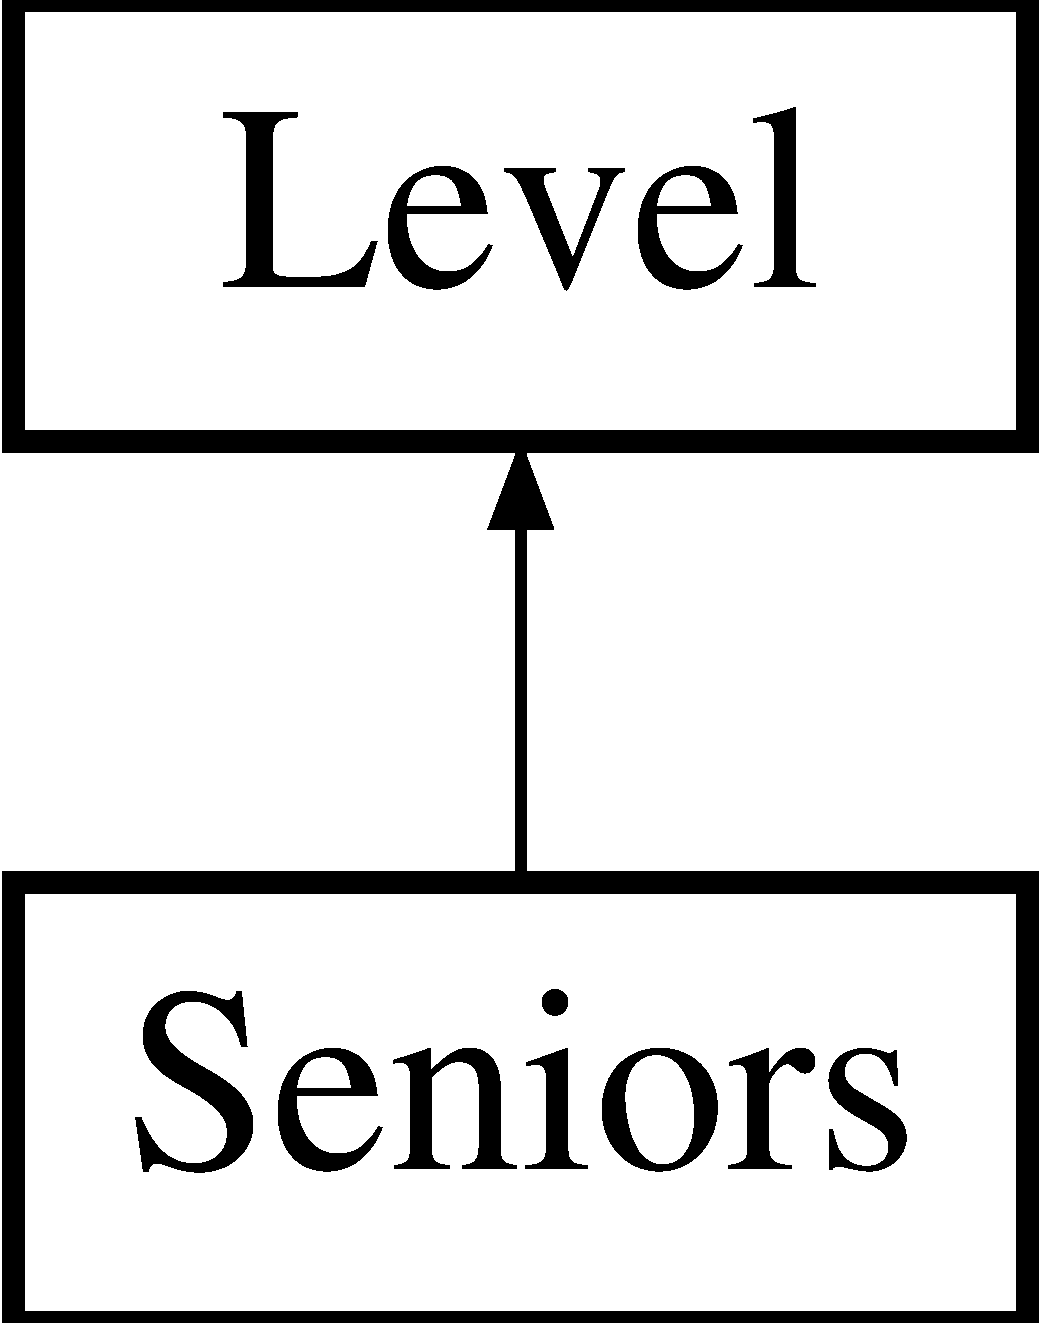
\includegraphics[height=2.000000cm]{class_seniors}
\end{center}
\end{figure}
\subsection*{Public Member Functions}
\begin{DoxyCompactItemize}
\item 
\hyperlink{class_seniors_ae02d7a048872847e295db59af893798a}{Seniors} ()
\begin{DoxyCompactList}\small\item\em Default Constructor. \end{DoxyCompactList}\item 
\hyperlink{class_seniors_a3063e1ce430ade54ec6b7a41a51bf942}{$\sim$\+Seniors} ()
\begin{DoxyCompactList}\small\item\em Destructor. \end{DoxyCompactList}\item 
\hyperlink{class_seniors_afb61156464d704b00aff866de6ee727a}{Seniors} (const \hyperlink{class_seniors}{Seniors} \&seniors)
\begin{DoxyCompactList}\small\item\em Copy Constructor. \end{DoxyCompactList}\item 
\hyperlink{class_seniors}{Seniors} \& \hyperlink{class_seniors_a6ec55b45cb67c34004c38a36fc3f8e64}{operator=} (const \hyperlink{class_seniors}{Seniors} \&seniors)
\begin{DoxyCompactList}\small\item\em Copy Operator. \end{DoxyCompactList}\item 
virtual unsigned int \hyperlink{class_seniors_a856a5d37a9dbda1e1b3ad8eb90db1f2a}{get\+Max\+Age} ()
\begin{DoxyCompactList}\small\item\em Gets the member variable age\+\_\+max. \end{DoxyCompactList}\item 
virtual unsigned int \hyperlink{class_seniors_a1843edaf8811f4728f76c11c79fe5450}{get\+Min\+Age} ()
\begin{DoxyCompactList}\small\item\em Gets the member variable age\+\_\+min. \end{DoxyCompactList}\item 
virtual bool \hyperlink{class_seniors_a4ee5683212625ee909b5c04d08bc8823}{add\+Player} (\hyperlink{class_player}{Player} $\ast$player)
\begin{DoxyCompactList}\small\item\em Adds a new \hyperlink{class_player}{Player} to this \hyperlink{class_level}{Level}. \end{DoxyCompactList}\item 
virtual void \hyperlink{class_seniors_a671c22ddbb0c2df27adf12364db0380a}{showplayers} () const
\begin{DoxyCompactList}\small\item\em Outputs the Players of this \hyperlink{class_level}{Level} on the screen. \end{DoxyCompactList}\item 
virtual void \hyperlink{class_seniors_a1f993a8ff143cc2e6dee8f3c81ed4cf3}{showtrainings} () const
\begin{DoxyCompactList}\small\item\em Outputs the Trainings of this \hyperlink{class_level}{Level} on the screen. \end{DoxyCompactList}\item 
virtual void \hyperlink{class_seniors_a5782adf80e1221220aa9e7bcaca5a3e3}{showtournaments} () const
\begin{DoxyCompactList}\small\item\em Outputs the Tournaments of this \hyperlink{class_level}{Level} on the screen. \end{DoxyCompactList}\item 
virtual vector$<$ string $>$ \hyperlink{class_seniors_a3b2fbe1e5d735c7659a195cea6333a0b}{get\+Call} (unsigned int size)
\begin{DoxyCompactList}\small\item\em Gets names of players to be called to a \hyperlink{class_tournament}{Tournament}. \end{DoxyCompactList}\end{DoxyCompactItemize}


\subsection{Detailed Description}
Holds all the information about the \hyperlink{class_level}{Level} \hyperlink{class_seniors}{Seniors}. 

Definition at line 23 of file Seniors.\+h.



\subsection{Constructor \& Destructor Documentation}
\hypertarget{class_seniors_ae02d7a048872847e295db59af893798a}{}\label{class_seniors_ae02d7a048872847e295db59af893798a} 
\index{Seniors@{Seniors}!Seniors@{Seniors}}
\index{Seniors@{Seniors}!Seniors@{Seniors}}
\subsubsection{\texorpdfstring{Seniors()}{Seniors()}\hspace{0.1cm}{\footnotesize\ttfamily [1/2]}}
{\footnotesize\ttfamily Seniors\+::\+Seniors (\begin{DoxyParamCaption}{ }\end{DoxyParamCaption})\hspace{0.3cm}{\ttfamily [inline]}}



Default Constructor. 



Definition at line 29 of file Seniors.\+h.

\hypertarget{class_seniors_a3063e1ce430ade54ec6b7a41a51bf942}{}\label{class_seniors_a3063e1ce430ade54ec6b7a41a51bf942} 
\index{Seniors@{Seniors}!````~Seniors@{$\sim$\+Seniors}}
\index{````~Seniors@{$\sim$\+Seniors}!Seniors@{Seniors}}
\subsubsection{\texorpdfstring{$\sim$\+Seniors()}{~Seniors()}}
{\footnotesize\ttfamily Seniors\+::$\sim$\+Seniors (\begin{DoxyParamCaption}{ }\end{DoxyParamCaption})\hspace{0.3cm}{\ttfamily [inline]}}



Destructor. 



Definition at line 33 of file Seniors.\+h.

\hypertarget{class_seniors_afb61156464d704b00aff866de6ee727a}{}\label{class_seniors_afb61156464d704b00aff866de6ee727a} 
\index{Seniors@{Seniors}!Seniors@{Seniors}}
\index{Seniors@{Seniors}!Seniors@{Seniors}}
\subsubsection{\texorpdfstring{Seniors()}{Seniors()}\hspace{0.1cm}{\footnotesize\ttfamily [2/2]}}
{\footnotesize\ttfamily Seniors\+::\+Seniors (\begin{DoxyParamCaption}\item[{const \hyperlink{class_seniors}{Seniors} \&}]{seniors }\end{DoxyParamCaption})\hspace{0.3cm}{\ttfamily [inline]}}



Copy Constructor. 


\begin{DoxyParams}{Parameters}
{\em seniors} & Object of class to be copied \\
\hline
\end{DoxyParams}


Definition at line 38 of file Seniors.\+h.



\subsection{Member Function Documentation}
\hypertarget{class_seniors_a4ee5683212625ee909b5c04d08bc8823}{}\label{class_seniors_a4ee5683212625ee909b5c04d08bc8823} 
\index{Seniors@{Seniors}!add\+Player@{add\+Player}}
\index{add\+Player@{add\+Player}!Seniors@{Seniors}}
\subsubsection{\texorpdfstring{add\+Player()}{addPlayer()}}
{\footnotesize\ttfamily bool Seniors\+::add\+Player (\begin{DoxyParamCaption}\item[{\hyperlink{class_player}{Player} $\ast$}]{player }\end{DoxyParamCaption})\hspace{0.3cm}{\ttfamily [virtual]}}



Adds a new \hyperlink{class_player}{Player} to this \hyperlink{class_level}{Level}. 


\begin{DoxyParams}{Parameters}
{\em player} & Pointer to \hyperlink{class_player}{Player} to be added \\
\hline
\end{DoxyParams}
\begin{DoxyReturn}{Returns}
true if it was added successfuly, false if not 
\end{DoxyReturn}


Reimplemented from \hyperlink{class_level_a66290778fa4bcd2f29b9ff3e605b2902}{Level}.



Definition at line 15 of file Seniors.\+cpp.

\hypertarget{class_seniors_a3b2fbe1e5d735c7659a195cea6333a0b}{}\label{class_seniors_a3b2fbe1e5d735c7659a195cea6333a0b} 
\index{Seniors@{Seniors}!get\+Call@{get\+Call}}
\index{get\+Call@{get\+Call}!Seniors@{Seniors}}
\subsubsection{\texorpdfstring{get\+Call()}{getCall()}}
{\footnotesize\ttfamily vector$<$ string $>$ Seniors\+::get\+Call (\begin{DoxyParamCaption}\item[{unsigned int}]{size }\end{DoxyParamCaption})\hspace{0.3cm}{\ttfamily [virtual]}}



Gets names of players to be called to a \hyperlink{class_tournament}{Tournament}. 


\begin{DoxyParams}{Parameters}
{\em size} & How many players to be called \\
\hline
\end{DoxyParams}
\begin{DoxyReturn}{Returns}
Vector with names of Players to be called 
\end{DoxyReturn}


Implements \hyperlink{class_level_ac118b390f16a75b9a0e9df198b3190ad}{Level}.



Definition at line 79 of file Seniors.\+cpp.

\hypertarget{class_seniors_a856a5d37a9dbda1e1b3ad8eb90db1f2a}{}\label{class_seniors_a856a5d37a9dbda1e1b3ad8eb90db1f2a} 
\index{Seniors@{Seniors}!get\+Max\+Age@{get\+Max\+Age}}
\index{get\+Max\+Age@{get\+Max\+Age}!Seniors@{Seniors}}
\subsubsection{\texorpdfstring{get\+Max\+Age()}{getMaxAge()}}
{\footnotesize\ttfamily virtual unsigned int Seniors\+::get\+Max\+Age (\begin{DoxyParamCaption}{ }\end{DoxyParamCaption})\hspace{0.3cm}{\ttfamily [inline]}, {\ttfamily [virtual]}}



Gets the member variable age\+\_\+max. 

\begin{DoxyReturn}{Returns}
age\+\_\+max (member variable) 
\end{DoxyReturn}


Implements \hyperlink{class_level_ae7b28ba0cb8d49372c4657fbe42706e1}{Level}.



Definition at line 49 of file Seniors.\+h.

\hypertarget{class_seniors_a1843edaf8811f4728f76c11c79fe5450}{}\label{class_seniors_a1843edaf8811f4728f76c11c79fe5450} 
\index{Seniors@{Seniors}!get\+Min\+Age@{get\+Min\+Age}}
\index{get\+Min\+Age@{get\+Min\+Age}!Seniors@{Seniors}}
\subsubsection{\texorpdfstring{get\+Min\+Age()}{getMinAge()}}
{\footnotesize\ttfamily virtual unsigned int Seniors\+::get\+Min\+Age (\begin{DoxyParamCaption}{ }\end{DoxyParamCaption})\hspace{0.3cm}{\ttfamily [inline]}, {\ttfamily [virtual]}}



Gets the member variable age\+\_\+min. 

\begin{DoxyReturn}{Returns}
age\+\_\+min (member variable) 
\end{DoxyReturn}


Implements \hyperlink{class_level_a161cf8c238fd499c112d90504cb6f587}{Level}.



Definition at line 54 of file Seniors.\+h.

\hypertarget{class_seniors_a6ec55b45cb67c34004c38a36fc3f8e64}{}\label{class_seniors_a6ec55b45cb67c34004c38a36fc3f8e64} 
\index{Seniors@{Seniors}!operator=@{operator=}}
\index{operator=@{operator=}!Seniors@{Seniors}}
\subsubsection{\texorpdfstring{operator=()}{operator=()}}
{\footnotesize\ttfamily \hyperlink{class_seniors}{Seniors}\& Seniors\+::operator= (\begin{DoxyParamCaption}\item[{const \hyperlink{class_seniors}{Seniors} \&}]{seniors }\end{DoxyParamCaption})\hspace{0.3cm}{\ttfamily [inline]}}



Copy Operator. 


\begin{DoxyParams}{Parameters}
{\em seniors} & Object of class to be copied\\
\hline
\end{DoxyParams}
Calls the base class \hyperlink{class_level_a60eb04b65c900ae8dddf3d6251fac7b1}{Level\+::operator=} 

Definition at line 44 of file Seniors.\+h.

\hypertarget{class_seniors_a671c22ddbb0c2df27adf12364db0380a}{}\label{class_seniors_a671c22ddbb0c2df27adf12364db0380a} 
\index{Seniors@{Seniors}!showplayers@{showplayers}}
\index{showplayers@{showplayers}!Seniors@{Seniors}}
\subsubsection{\texorpdfstring{showplayers()}{showplayers()}}
{\footnotesize\ttfamily void Seniors\+::showplayers (\begin{DoxyParamCaption}{ }\end{DoxyParamCaption}) const\hspace{0.3cm}{\ttfamily [virtual]}}



Outputs the Players of this \hyperlink{class_level}{Level} on the screen. 



Reimplemented from \hyperlink{class_level_a40d22b376e72950a07de5e0a9e288029}{Level}.



Definition at line 29 of file Seniors.\+cpp.

\hypertarget{class_seniors_a5782adf80e1221220aa9e7bcaca5a3e3}{}\label{class_seniors_a5782adf80e1221220aa9e7bcaca5a3e3} 
\index{Seniors@{Seniors}!showtournaments@{showtournaments}}
\index{showtournaments@{showtournaments}!Seniors@{Seniors}}
\subsubsection{\texorpdfstring{showtournaments()}{showtournaments()}}
{\footnotesize\ttfamily void Seniors\+::showtournaments (\begin{DoxyParamCaption}{ }\end{DoxyParamCaption}) const\hspace{0.3cm}{\ttfamily [virtual]}}



Outputs the Tournaments of this \hyperlink{class_level}{Level} on the screen. 



Reimplemented from \hyperlink{class_level_a757c4547f3b8f7c7ecb02c7e0e6cd7c9}{Level}.



Definition at line 45 of file Seniors.\+cpp.

\hypertarget{class_seniors_a1f993a8ff143cc2e6dee8f3c81ed4cf3}{}\label{class_seniors_a1f993a8ff143cc2e6dee8f3c81ed4cf3} 
\index{Seniors@{Seniors}!showtrainings@{showtrainings}}
\index{showtrainings@{showtrainings}!Seniors@{Seniors}}
\subsubsection{\texorpdfstring{showtrainings()}{showtrainings()}}
{\footnotesize\ttfamily void Seniors\+::showtrainings (\begin{DoxyParamCaption}{ }\end{DoxyParamCaption}) const\hspace{0.3cm}{\ttfamily [virtual]}}



Outputs the Trainings of this \hyperlink{class_level}{Level} on the screen. 



Reimplemented from \hyperlink{class_level_a4101cb725b1fd0c0836834c92b190363}{Level}.



Definition at line 37 of file Seniors.\+cpp.



The documentation for this class was generated from the following files\+:\begin{DoxyCompactItemize}
\item 
/home/oco/\+Documents/\+Cprojects/\+Athletes/projecto -\/ V2/\+Headers/\hyperlink{_seniors_8h}{Seniors.\+h}\item 
/home/oco/\+Documents/\+Cprojects/\+Athletes/projecto -\/ V2/\+Source/\hyperlink{_seniors_8cpp}{Seniors.\+cpp}\end{DoxyCompactItemize}

\hypertarget{class_tournament}{}\section{Tournament Class Reference}
\label{class_tournament}\index{Tournament@{Tournament}}


Used to host information about a single \hyperlink{class_tournament}{Tournament}.  




{\ttfamily \#include $<$Tournament.\+h$>$}

Inheritance diagram for Tournament\+:\begin{figure}[H]
\begin{center}
\leavevmode
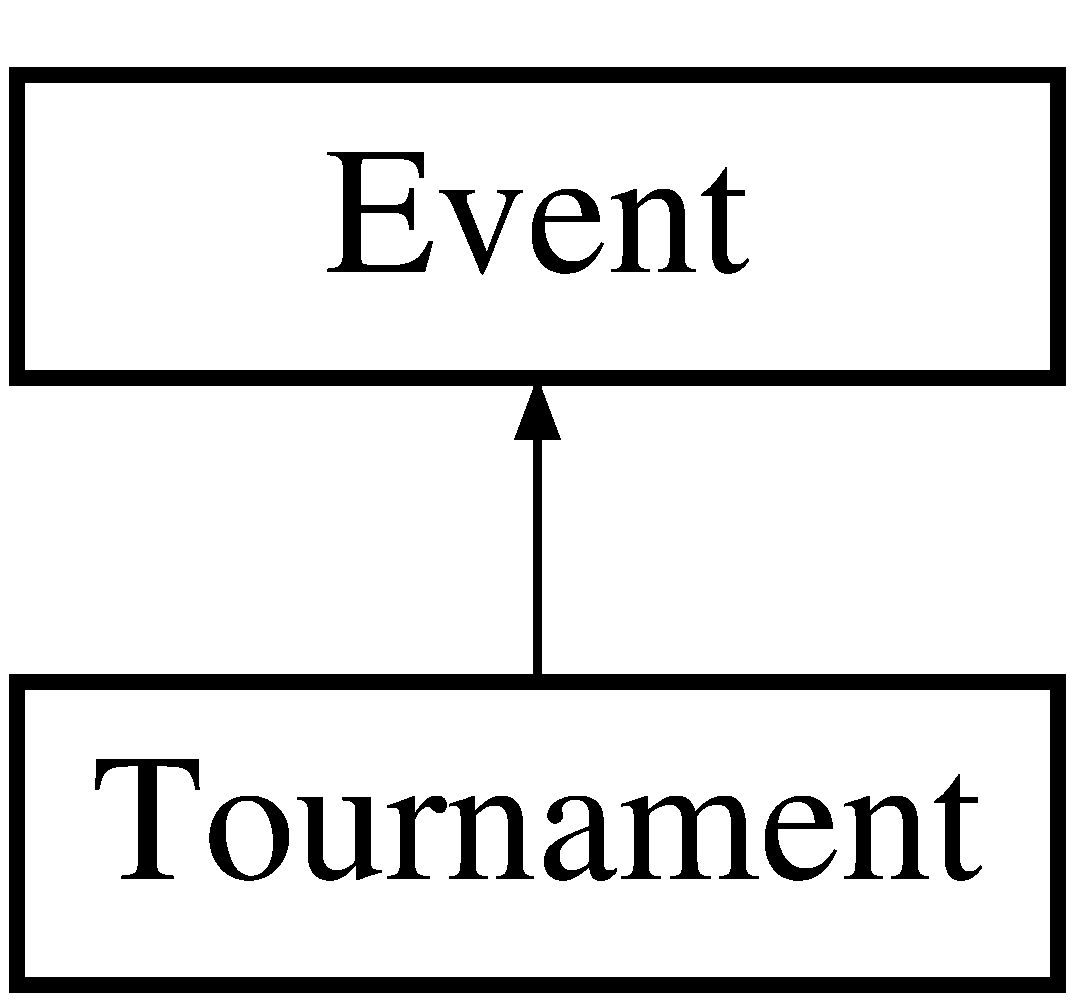
\includegraphics[height=2.000000cm]{class_tournament}
\end{center}
\end{figure}
\subsection*{Public Member Functions}
\begin{DoxyCompactItemize}
\item 
\hyperlink{class_tournament_a87cc832c6612caebcab61d1bea7ef1ac}{Tournament} ()
\begin{DoxyCompactList}\small\item\em Default Constructor. \end{DoxyCompactList}\item 
virtual \hyperlink{class_tournament_a255677d318362ae4dc23b9d6a3359f61}{$\sim$\+Tournament} ()
\begin{DoxyCompactList}\small\item\em Destructor. \end{DoxyCompactList}\item 
\hyperlink{class_tournament_a653ee8a664677bf0f757234150fa71f8}{Tournament} (const \hyperlink{class_tournament}{Tournament} \&tournament)
\begin{DoxyCompactList}\small\item\em Copy Constructor. \end{DoxyCompactList}\item 
\hyperlink{class_tournament}{Tournament} \& \hyperlink{class_tournament_a0eadb353ccff0b3c64b19d65f3353771}{operator=} (const \hyperlink{class_tournament}{Tournament} \&tournament)
\begin{DoxyCompactList}\small\item\em Copy Operator. \end{DoxyCompactList}\item 
\hyperlink{class_tournament_a38dbc53e1d0f1eaf6b661169db87c270}{Tournament} (\hyperlink{class_event}{Event} $\ast$ev)
\begin{DoxyCompactList}\small\item\em Pointer Copy Constructor. \end{DoxyCompactList}\item 
\hyperlink{class_tournament_a84c5301c50e0c4ac263ed3d74fa7c8c5}{Tournament} (\hyperlink{class_date}{Date} day, bool major)
\begin{DoxyCompactList}\small\item\em Partial Constructor. \end{DoxyCompactList}\item 
virtual bool \hyperlink{class_tournament_ab6fde765568ea9779fc10f0f2811c163}{Istraining} () const
\begin{DoxyCompactList}\small\item\em Checks if this \hyperlink{class_event}{Event} is a \hyperlink{class_training}{Training}. \end{DoxyCompactList}\item 
virtual void \hyperlink{class_tournament_a35bd5292194edb5d5c220838b68cda75}{show} () const
\begin{DoxyCompactList}\small\item\em Used to print the \hyperlink{class_tournament}{Tournament} on the screen. \end{DoxyCompactList}\item 
virtual bool \hyperlink{class_tournament_a62adb322a6d5268d4ec3e267570ff4ed}{is\+Game} () const
\begin{DoxyCompactList}\small\item\em Checks if the \hyperlink{class_training}{Training} was a game. \end{DoxyCompactList}\item 
virtual unsigned int \hyperlink{class_tournament_ae021dc9d9aa7fb8b18bd065bfccc4b7e}{get\+Rank} () const
\begin{DoxyCompactList}\small\item\em Gets the rank achieved by the \hyperlink{class_level}{Level} at a \hyperlink{class_tournament}{Tournament}. \end{DoxyCompactList}\item 
virtual bool \hyperlink{class_tournament_af733baa05b3ae1465d6b5271929b5061}{is\+Major} () const
\begin{DoxyCompactList}\small\item\em Checks if \hyperlink{class_tournament}{Tournament} was a major \hyperlink{class_tournament}{Tournament}. \end{DoxyCompactList}\item 
virtual vector$<$ pair$<$ pair$<$ unsigned int, unsigned int $>$, string $>$ $>$ \hyperlink{class_tournament_abacd2d5489099f31a9688a7da4d64c40}{get\+Results} () const
\begin{DoxyCompactList}\small\item\em Gets the results of the \hyperlink{class_level}{Level} in the \hyperlink{class_tournament}{Tournament}. \end{DoxyCompactList}\item 
virtual void \hyperlink{class_tournament_acab9ee32169ba590f4ffdb5b59b28a86}{set\+Results} (vector$<$ pair$<$ pair$<$ unsigned int, unsigned int $>$, string $>$$>$ results)
\begin{DoxyCompactList}\small\item\em Changes the results obtained on the \hyperlink{class_tournament}{Tournament}. \end{DoxyCompactList}\item 
virtual void \hyperlink{class_tournament_a724f8fb0c0507975b6bb4817d8b5de7d}{set\+Rank} (unsigned int rank)
\begin{DoxyCompactList}\small\item\em Changes the rank achieved on the \hyperlink{class_tournament}{Tournament}. \end{DoxyCompactList}\item 
virtual void \hyperlink{class_tournament_a4aa375c287d890b9117a91058dcffb0c}{writetofile} (ostream \&out) const
\begin{DoxyCompactList}\small\item\em Writes the \hyperlink{class_tournament}{Tournament} to a file using operator$<$$<$. \end{DoxyCompactList}\end{DoxyCompactItemize}
\subsection*{Friends}
\begin{DoxyCompactItemize}
\item 
ostream \& \hyperlink{class_tournament_a732b99f4a91ce76bb3db57cffd96f441}{operator$<$$<$} (ostream \&out, const \hyperlink{class_tournament}{Tournament} \&tournament)
\begin{DoxyCompactList}\small\item\em Used to write the \hyperlink{class_tournament}{Tournament} to an Output Stream. \end{DoxyCompactList}\item 
istream \& \hyperlink{class_tournament_a35e43e0ee6981515ba4442efa8cac7a7}{operator$>$$>$} (istream \&in, \hyperlink{class_tournament}{Tournament} \&tournament)
\begin{DoxyCompactList}\small\item\em Used to read the \hyperlink{class_tournament}{Tournament} from an Input Stream. \end{DoxyCompactList}\end{DoxyCompactItemize}


\subsection{Detailed Description}
Used to host information about a single \hyperlink{class_tournament}{Tournament}. 

Definition at line 25 of file Tournament.\+h.



\subsection{Constructor \& Destructor Documentation}
\hypertarget{class_tournament_a87cc832c6612caebcab61d1bea7ef1ac}{}\label{class_tournament_a87cc832c6612caebcab61d1bea7ef1ac} 
\index{Tournament@{Tournament}!Tournament@{Tournament}}
\index{Tournament@{Tournament}!Tournament@{Tournament}}
\subsubsection{\texorpdfstring{Tournament()}{Tournament()}\hspace{0.1cm}{\footnotesize\ttfamily [1/4]}}
{\footnotesize\ttfamily Tournament\+::\+Tournament (\begin{DoxyParamCaption}{ }\end{DoxyParamCaption})\hspace{0.3cm}{\ttfamily [inline]}}



Default Constructor. 



Definition at line 34 of file Tournament.\+h.

\hypertarget{class_tournament_a255677d318362ae4dc23b9d6a3359f61}{}\label{class_tournament_a255677d318362ae4dc23b9d6a3359f61} 
\index{Tournament@{Tournament}!````~Tournament@{$\sim$\+Tournament}}
\index{````~Tournament@{$\sim$\+Tournament}!Tournament@{Tournament}}
\subsubsection{\texorpdfstring{$\sim$\+Tournament()}{~Tournament()}}
{\footnotesize\ttfamily virtual Tournament\+::$\sim$\+Tournament (\begin{DoxyParamCaption}{ }\end{DoxyParamCaption})\hspace{0.3cm}{\ttfamily [inline]}, {\ttfamily [virtual]}}



Destructor. 



Definition at line 38 of file Tournament.\+h.

\hypertarget{class_tournament_a653ee8a664677bf0f757234150fa71f8}{}\label{class_tournament_a653ee8a664677bf0f757234150fa71f8} 
\index{Tournament@{Tournament}!Tournament@{Tournament}}
\index{Tournament@{Tournament}!Tournament@{Tournament}}
\subsubsection{\texorpdfstring{Tournament()}{Tournament()}\hspace{0.1cm}{\footnotesize\ttfamily [2/4]}}
{\footnotesize\ttfamily Tournament\+::\+Tournament (\begin{DoxyParamCaption}\item[{const \hyperlink{class_tournament}{Tournament} \&}]{tournament }\end{DoxyParamCaption})}



Copy Constructor. 


\begin{DoxyParams}{Parameters}
{\em tournament} & \hyperlink{class_tournament}{Tournament} object to be copied \\
\hline
\end{DoxyParams}


Definition at line 11 of file Tournament.\+cpp.

\hypertarget{class_tournament_a38dbc53e1d0f1eaf6b661169db87c270}{}\label{class_tournament_a38dbc53e1d0f1eaf6b661169db87c270} 
\index{Tournament@{Tournament}!Tournament@{Tournament}}
\index{Tournament@{Tournament}!Tournament@{Tournament}}
\subsubsection{\texorpdfstring{Tournament()}{Tournament()}\hspace{0.1cm}{\footnotesize\ttfamily [3/4]}}
{\footnotesize\ttfamily Tournament\+::\+Tournament (\begin{DoxyParamCaption}\item[{\hyperlink{class_event}{Event} $\ast$}]{ev }\end{DoxyParamCaption})}



Pointer Copy Constructor. 


\begin{DoxyParams}{Parameters}
{\em ev} & Pointer to \hyperlink{class_training}{Training} object to be copied \\
\hline
\end{DoxyParams}


Definition at line 30 of file Tournament.\+cpp.

\hypertarget{class_tournament_a84c5301c50e0c4ac263ed3d74fa7c8c5}{}\label{class_tournament_a84c5301c50e0c4ac263ed3d74fa7c8c5} 
\index{Tournament@{Tournament}!Tournament@{Tournament}}
\index{Tournament@{Tournament}!Tournament@{Tournament}}
\subsubsection{\texorpdfstring{Tournament()}{Tournament()}\hspace{0.1cm}{\footnotesize\ttfamily [4/4]}}
{\footnotesize\ttfamily Tournament\+::\+Tournament (\begin{DoxyParamCaption}\item[{\hyperlink{class_date}{Date}}]{day,  }\item[{bool}]{major }\end{DoxyParamCaption})\hspace{0.3cm}{\ttfamily [inline]}}



Partial Constructor. 


\begin{DoxyParams}{Parameters}
{\em day} & \hyperlink{class_date}{Date} of the \hyperlink{class_event}{Event} \\
\hline
{\em major} & Whether it was a Major \hyperlink{class_tournament}{Tournament} or not \\
\hline
\end{DoxyParams}


Definition at line 59 of file Tournament.\+h.



\subsection{Member Function Documentation}
\hypertarget{class_tournament_ae021dc9d9aa7fb8b18bd065bfccc4b7e}{}\label{class_tournament_ae021dc9d9aa7fb8b18bd065bfccc4b7e} 
\index{Tournament@{Tournament}!get\+Rank@{get\+Rank}}
\index{get\+Rank@{get\+Rank}!Tournament@{Tournament}}
\subsubsection{\texorpdfstring{get\+Rank()}{getRank()}}
{\footnotesize\ttfamily virtual unsigned int Tournament\+::get\+Rank (\begin{DoxyParamCaption}{ }\end{DoxyParamCaption}) const\hspace{0.3cm}{\ttfamily [inline]}, {\ttfamily [virtual]}}



Gets the rank achieved by the \hyperlink{class_level}{Level} at a \hyperlink{class_tournament}{Tournament}. 

\begin{DoxyReturn}{Returns}
rank (member variable) 
\end{DoxyReturn}


Implements \hyperlink{class_event_ab267b8e94c78ca51636792d75101acb5}{Event}.



Definition at line 78 of file Tournament.\+h.

\hypertarget{class_tournament_abacd2d5489099f31a9688a7da4d64c40}{}\label{class_tournament_abacd2d5489099f31a9688a7da4d64c40} 
\index{Tournament@{Tournament}!get\+Results@{get\+Results}}
\index{get\+Results@{get\+Results}!Tournament@{Tournament}}
\subsubsection{\texorpdfstring{get\+Results()}{getResults()}}
{\footnotesize\ttfamily virtual vector$<$pair$<$pair$<$unsigned int, unsigned int$>$, string $>$ $>$ Tournament\+::get\+Results (\begin{DoxyParamCaption}{ }\end{DoxyParamCaption}) const\hspace{0.3cm}{\ttfamily [inline]}, {\ttfamily [virtual]}}



Gets the results of the \hyperlink{class_level}{Level} in the \hyperlink{class_tournament}{Tournament}. 

\begin{DoxyReturn}{Returns}
results (member variable) 
\end{DoxyReturn}


Implements \hyperlink{class_event_a9d29f8c725da32b5fbf70ccf7961f02b}{Event}.



Definition at line 88 of file Tournament.\+h.

\hypertarget{class_tournament_a62adb322a6d5268d4ec3e267570ff4ed}{}\label{class_tournament_a62adb322a6d5268d4ec3e267570ff4ed} 
\index{Tournament@{Tournament}!is\+Game@{is\+Game}}
\index{is\+Game@{is\+Game}!Tournament@{Tournament}}
\subsubsection{\texorpdfstring{is\+Game()}{isGame()}}
{\footnotesize\ttfamily virtual bool Tournament\+::is\+Game (\begin{DoxyParamCaption}{ }\end{DoxyParamCaption}) const\hspace{0.3cm}{\ttfamily [inline]}, {\ttfamily [virtual]}}



Checks if the \hyperlink{class_training}{Training} was a game. 

\begin{DoxyReturn}{Returns}
False since all objects of this class have no game parameter 
\end{DoxyReturn}


Implements \hyperlink{class_event_add36e9739215f6744040c11de50b26b7}{Event}.



Definition at line 73 of file Tournament.\+h.

\hypertarget{class_tournament_af733baa05b3ae1465d6b5271929b5061}{}\label{class_tournament_af733baa05b3ae1465d6b5271929b5061} 
\index{Tournament@{Tournament}!is\+Major@{is\+Major}}
\index{is\+Major@{is\+Major}!Tournament@{Tournament}}
\subsubsection{\texorpdfstring{is\+Major()}{isMajor()}}
{\footnotesize\ttfamily virtual bool Tournament\+::is\+Major (\begin{DoxyParamCaption}{ }\end{DoxyParamCaption}) const\hspace{0.3cm}{\ttfamily [inline]}, {\ttfamily [virtual]}}



Checks if \hyperlink{class_tournament}{Tournament} was a major \hyperlink{class_tournament}{Tournament}. 

\begin{DoxyReturn}{Returns}
major (member variable) 
\end{DoxyReturn}


Implements \hyperlink{class_event_ad1a1a9cb471d664a2ca99effc102259b}{Event}.



Definition at line 83 of file Tournament.\+h.

\hypertarget{class_tournament_ab6fde765568ea9779fc10f0f2811c163}{}\label{class_tournament_ab6fde765568ea9779fc10f0f2811c163} 
\index{Tournament@{Tournament}!Istraining@{Istraining}}
\index{Istraining@{Istraining}!Tournament@{Tournament}}
\subsubsection{\texorpdfstring{Istraining()}{Istraining()}}
{\footnotesize\ttfamily virtual bool Tournament\+::\+Istraining (\begin{DoxyParamCaption}{ }\end{DoxyParamCaption}) const\hspace{0.3cm}{\ttfamily [inline]}, {\ttfamily [virtual]}}



Checks if this \hyperlink{class_event}{Event} is a \hyperlink{class_training}{Training}. 

\begin{DoxyReturn}{Returns}
False since all objects of this class are Tournaments 
\end{DoxyReturn}


Implements \hyperlink{class_event_a08af9b350f32520dca26d552d6f415b2}{Event}.



Definition at line 64 of file Tournament.\+h.

\hypertarget{class_tournament_a0eadb353ccff0b3c64b19d65f3353771}{}\label{class_tournament_a0eadb353ccff0b3c64b19d65f3353771} 
\index{Tournament@{Tournament}!operator=@{operator=}}
\index{operator=@{operator=}!Tournament@{Tournament}}
\subsubsection{\texorpdfstring{operator=()}{operator=()}}
{\footnotesize\ttfamily \hyperlink{class_tournament}{Tournament} \& Tournament\+::operator= (\begin{DoxyParamCaption}\item[{const \hyperlink{class_tournament}{Tournament} \&}]{tournament }\end{DoxyParamCaption})}



Copy Operator. 


\begin{DoxyParams}{Parameters}
{\em tournament} & \hyperlink{class_tournament}{Tournament} object to be copied \\
\hline
\end{DoxyParams}


Definition at line 19 of file Tournament.\+cpp.

\hypertarget{class_tournament_a724f8fb0c0507975b6bb4817d8b5de7d}{}\label{class_tournament_a724f8fb0c0507975b6bb4817d8b5de7d} 
\index{Tournament@{Tournament}!set\+Rank@{set\+Rank}}
\index{set\+Rank@{set\+Rank}!Tournament@{Tournament}}
\subsubsection{\texorpdfstring{set\+Rank()}{setRank()}}
{\footnotesize\ttfamily virtual void Tournament\+::set\+Rank (\begin{DoxyParamCaption}\item[{unsigned int}]{rank }\end{DoxyParamCaption})\hspace{0.3cm}{\ttfamily [inline]}, {\ttfamily [virtual]}}



Changes the rank achieved on the \hyperlink{class_tournament}{Tournament}. 


\begin{DoxyParams}{Parameters}
{\em rank} & Value to be changed into \\
\hline
\end{DoxyParams}


Implements \hyperlink{class_event_a5bccaba301e9038957ec4138df404524}{Event}.



Definition at line 98 of file Tournament.\+h.

\hypertarget{class_tournament_acab9ee32169ba590f4ffdb5b59b28a86}{}\label{class_tournament_acab9ee32169ba590f4ffdb5b59b28a86} 
\index{Tournament@{Tournament}!set\+Results@{set\+Results}}
\index{set\+Results@{set\+Results}!Tournament@{Tournament}}
\subsubsection{\texorpdfstring{set\+Results()}{setResults()}}
{\footnotesize\ttfamily virtual void Tournament\+::set\+Results (\begin{DoxyParamCaption}\item[{vector$<$ pair$<$ pair$<$ unsigned int, unsigned int $>$, string $>$$>$}]{results }\end{DoxyParamCaption})\hspace{0.3cm}{\ttfamily [inline]}, {\ttfamily [virtual]}}



Changes the results obtained on the \hyperlink{class_tournament}{Tournament}. 


\begin{DoxyParams}{Parameters}
{\em results} & Value to be changed into \\
\hline
\end{DoxyParams}


Implements \hyperlink{class_event_a5ddb261642035be78677d668f9238339}{Event}.



Definition at line 93 of file Tournament.\+h.

\hypertarget{class_tournament_a35bd5292194edb5d5c220838b68cda75}{}\label{class_tournament_a35bd5292194edb5d5c220838b68cda75} 
\index{Tournament@{Tournament}!show@{show}}
\index{show@{show}!Tournament@{Tournament}}
\subsubsection{\texorpdfstring{show()}{show()}}
{\footnotesize\ttfamily void Tournament\+::show (\begin{DoxyParamCaption}{ }\end{DoxyParamCaption}) const\hspace{0.3cm}{\ttfamily [virtual]}}



Used to print the \hyperlink{class_tournament}{Tournament} on the screen. 



Implements \hyperlink{class_event_af53c2db83404a045087a271ed3c2604f}{Event}.



Definition at line 40 of file Tournament.\+cpp.

\hypertarget{class_tournament_a4aa375c287d890b9117a91058dcffb0c}{}\label{class_tournament_a4aa375c287d890b9117a91058dcffb0c} 
\index{Tournament@{Tournament}!writetofile@{writetofile}}
\index{writetofile@{writetofile}!Tournament@{Tournament}}
\subsubsection{\texorpdfstring{writetofile()}{writetofile()}}
{\footnotesize\ttfamily virtual void Tournament\+::writetofile (\begin{DoxyParamCaption}\item[{ostream \&}]{out }\end{DoxyParamCaption}) const\hspace{0.3cm}{\ttfamily [inline]}, {\ttfamily [virtual]}}



Writes the \hyperlink{class_tournament}{Tournament} to a file using operator$<$$<$. 


\begin{DoxyParams}{Parameters}
{\em out} & File to write to \\
\hline
\end{DoxyParams}


Implements \hyperlink{class_event_a0c263fb7398dc2f0969a2bb22b47a40a}{Event}.



Definition at line 117 of file Tournament.\+h.



\subsection{Friends And Related Function Documentation}
\hypertarget{class_tournament_a732b99f4a91ce76bb3db57cffd96f441}{}\label{class_tournament_a732b99f4a91ce76bb3db57cffd96f441} 
\index{Tournament@{Tournament}!operator$<$$<$@{operator$<$$<$}}
\index{operator$<$$<$@{operator$<$$<$}!Tournament@{Tournament}}
\subsubsection{\texorpdfstring{operator$<$$<$}{operator<<}}
{\footnotesize\ttfamily ostream\& operator$<$$<$ (\begin{DoxyParamCaption}\item[{ostream \&}]{out,  }\item[{const \hyperlink{class_tournament}{Tournament} \&}]{tournament }\end{DoxyParamCaption})\hspace{0.3cm}{\ttfamily [friend]}}



Used to write the \hyperlink{class_tournament}{Tournament} to an Output Stream. 


\begin{DoxyParams}{Parameters}
{\em out} & Output Stream to write the \hyperlink{class_tournament}{Tournament} to \\
\hline
{\em tournament} & \hyperlink{class_tournament}{Tournament} to be written on the Output Stream \\
\hline
\end{DoxyParams}
\begin{DoxyReturn}{Returns}
out (parameter) 
\end{DoxyReturn}


Definition at line 59 of file Tournament.\+cpp.

\hypertarget{class_tournament_a35e43e0ee6981515ba4442efa8cac7a7}{}\label{class_tournament_a35e43e0ee6981515ba4442efa8cac7a7} 
\index{Tournament@{Tournament}!operator$>$$>$@{operator$>$$>$}}
\index{operator$>$$>$@{operator$>$$>$}!Tournament@{Tournament}}
\subsubsection{\texorpdfstring{operator$>$$>$}{operator>>}}
{\footnotesize\ttfamily istream\& operator$>$$>$ (\begin{DoxyParamCaption}\item[{istream \&}]{in,  }\item[{\hyperlink{class_tournament}{Tournament} \&}]{tournament }\end{DoxyParamCaption})\hspace{0.3cm}{\ttfamily [friend]}}



Used to read the \hyperlink{class_tournament}{Tournament} from an Input Stream. 


\begin{DoxyParams}{Parameters}
{\em in} & Input Stream from which to read the \hyperlink{class_tournament}{Tournament} \\
\hline
{\em tournament} & \hyperlink{class_tournament}{Tournament} to be read from the Input Stream \\
\hline
\end{DoxyParams}
\begin{DoxyReturn}{Returns}
in (parameter) 
\end{DoxyReturn}


Definition at line 79 of file Tournament.\+cpp.



The documentation for this class was generated from the following files\+:\begin{DoxyCompactItemize}
\item 
/home/oco/\+Documents/\+Cprojects/\+Athletes/projecto -\/ V2/\+Headers/\hyperlink{_tournament_8h}{Tournament.\+h}\item 
/home/oco/\+Documents/\+Cprojects/\+Athletes/projecto -\/ V2/\+Source/\hyperlink{_tournament_8cpp}{Tournament.\+cpp}\end{DoxyCompactItemize}

\hypertarget{class_training}{}\section{Training Class Reference}
\label{class_training}\index{Training@{Training}}


Used to host information about a single \hyperlink{class_training}{Training}.  




{\ttfamily \#include $<$Training.\+h$>$}

Inheritance diagram for Training\+:\begin{figure}[H]
\begin{center}
\leavevmode
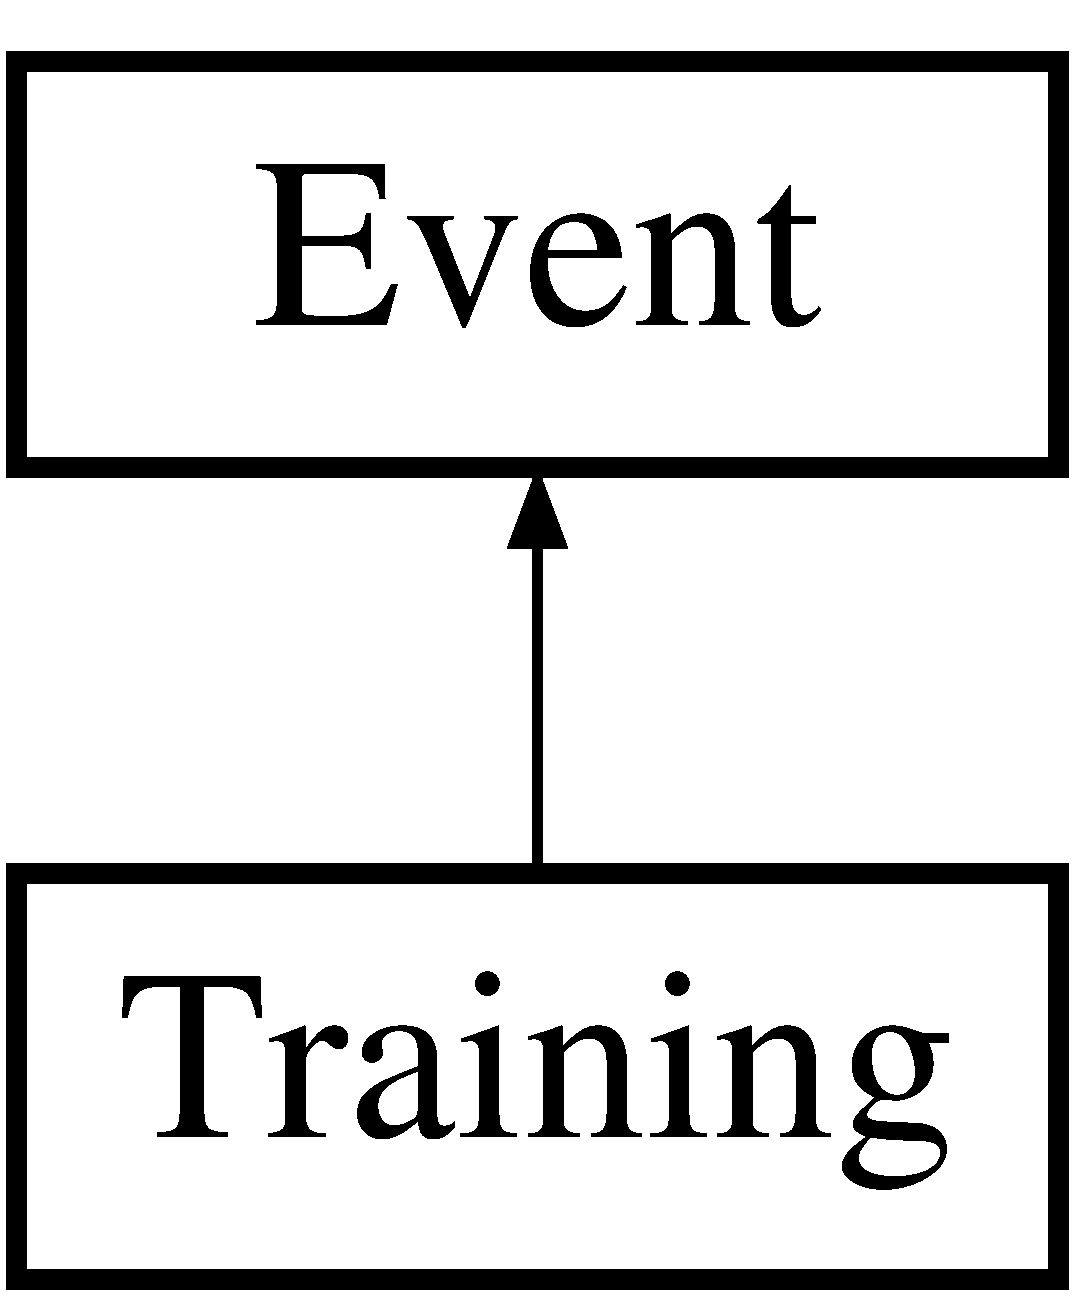
\includegraphics[height=2.000000cm]{class_training}
\end{center}
\end{figure}
\subsection*{Public Member Functions}
\begin{DoxyCompactItemize}
\item 
\hyperlink{class_training_af98b1bc7ed710e2fa008a72ad29dbdae}{Training} ()
\begin{DoxyCompactList}\small\item\em Default Constructor. \end{DoxyCompactList}\item 
virtual \hyperlink{class_training_a4a40f758a773c3c63d8558eaa78b1abd}{$\sim$\+Training} ()
\begin{DoxyCompactList}\small\item\em Destructor. \end{DoxyCompactList}\item 
\hyperlink{class_training_a923c500458737327f874067ffc7ca1c9}{Training} (const \hyperlink{class_training}{Training} \&training)
\begin{DoxyCompactList}\small\item\em Copy Constructor. \end{DoxyCompactList}\item 
\hyperlink{class_training}{Training} \& \hyperlink{class_training_aea6dff02f1a10d73ec15ceb310fb7b3f}{operator=} (const \hyperlink{class_training}{Training} \&training)
\begin{DoxyCompactList}\small\item\em Copy Operator. \end{DoxyCompactList}\item 
\hyperlink{class_training_ae39813d608325645cb3403160fc3b493}{Training} (\hyperlink{class_event}{Event} $\ast$ev)
\begin{DoxyCompactList}\small\item\em Pointer Copy Constructor. \end{DoxyCompactList}\item 
\hyperlink{class_training_a314d31d73f207b1c9cb2720da663d225}{Training} (\hyperlink{class_date}{Date} day, bool game)
\begin{DoxyCompactList}\small\item\em Partial Constructor. \end{DoxyCompactList}\item 
virtual bool \hyperlink{class_training_a55530cc22aa771cf3e452c7158b5396e}{is\+Game} () const
\begin{DoxyCompactList}\small\item\em Checks if the \hyperlink{class_training}{Training} was a game. \end{DoxyCompactList}\item 
virtual bool \hyperlink{class_training_ab70fe087f382d0de9dca69ce519be91e}{Istraining} () const
\begin{DoxyCompactList}\small\item\em Checks if this \hyperlink{class_event}{Event} is a \hyperlink{class_training}{Training}. \end{DoxyCompactList}\item 
virtual void \hyperlink{class_training_a9391fa1f4862855341d6243e75f9efef}{show} () const
\begin{DoxyCompactList}\small\item\em Prints the \hyperlink{class_training}{Training} on the screen. \end{DoxyCompactList}\item 
virtual unsigned int \hyperlink{class_training_ada723ff1f8340338a99e720a1b472334}{get\+Rank} () const
\begin{DoxyCompactList}\small\item\em Gets the rank achieved by the \hyperlink{class_level}{Level} at a \hyperlink{class_tournament}{Tournament}. \end{DoxyCompactList}\item 
virtual bool \hyperlink{class_training_aaf1c4d96664a16ca141dd5a3582f9426}{is\+Major} () const
\begin{DoxyCompactList}\small\item\em Checks if \hyperlink{class_tournament}{Tournament} was a major \hyperlink{class_tournament}{Tournament}. \end{DoxyCompactList}\item 
virtual vector$<$ pair$<$ pair$<$ unsigned int, unsigned int $>$, string $>$ $>$ \hyperlink{class_training_aa37e2baeee2b94cb15521e1768b99cc9}{get\+Results} () const
\begin{DoxyCompactList}\small\item\em Gets the results of the \hyperlink{class_level}{Level} in the \hyperlink{class_tournament}{Tournament}. \end{DoxyCompactList}\item 
virtual void \hyperlink{class_training_ad587b59c44a6e95a4e52f3d3f6b89480}{set\+Results} (vector$<$ pair$<$ pair$<$ unsigned int, unsigned int $>$, string $>$$>$ results)
\begin{DoxyCompactList}\small\item\em Does nothing since Trainings have no results. \end{DoxyCompactList}\item 
virtual void \hyperlink{class_training_a15d38322bd6a2ee8e17441bd4798b236}{set\+Rank} (unsigned int rank)
\begin{DoxyCompactList}\small\item\em Does nothing since Trainings have no rank. \end{DoxyCompactList}\item 
virtual void \hyperlink{class_training_a1755abc9faafbe06fb2825cb5f879016}{writetofile} (ostream \&out) const
\begin{DoxyCompactList}\small\item\em Writes the \hyperlink{class_training}{Training} to a file using operator$<$$<$. \end{DoxyCompactList}\end{DoxyCompactItemize}
\subsection*{Friends}
\begin{DoxyCompactItemize}
\item 
ostream \& \hyperlink{class_training_a2a462cd115913a43a1f4d7cbc8635c77}{operator$<$$<$} (ostream \&out, const \hyperlink{class_training}{Training} \&training)
\begin{DoxyCompactList}\small\item\em Used to write the \hyperlink{class_training}{Training} to an Output Stream. \end{DoxyCompactList}\item 
istream \& \hyperlink{class_training_ad76466bb3f1163c39b684ae14adf0ca1}{operator$>$$>$} (istream \&in, \hyperlink{class_training}{Training} \&training)
\begin{DoxyCompactList}\small\item\em Used to read the \hyperlink{class_training}{Training} from an Input Stream. \end{DoxyCompactList}\end{DoxyCompactItemize}


\subsection{Detailed Description}
Used to host information about a single \hyperlink{class_training}{Training}. 

Definition at line 19 of file Training.\+h.



\subsection{Constructor \& Destructor Documentation}
\hypertarget{class_training_af98b1bc7ed710e2fa008a72ad29dbdae}{}\label{class_training_af98b1bc7ed710e2fa008a72ad29dbdae} 
\index{Training@{Training}!Training@{Training}}
\index{Training@{Training}!Training@{Training}}
\subsubsection{\texorpdfstring{Training()}{Training()}\hspace{0.1cm}{\footnotesize\ttfamily [1/4]}}
{\footnotesize\ttfamily Training\+::\+Training (\begin{DoxyParamCaption}{ }\end{DoxyParamCaption})\hspace{0.3cm}{\ttfamily [inline]}}



Default Constructor. 



Definition at line 25 of file Training.\+h.

\hypertarget{class_training_a4a40f758a773c3c63d8558eaa78b1abd}{}\label{class_training_a4a40f758a773c3c63d8558eaa78b1abd} 
\index{Training@{Training}!````~Training@{$\sim$\+Training}}
\index{````~Training@{$\sim$\+Training}!Training@{Training}}
\subsubsection{\texorpdfstring{$\sim$\+Training()}{~Training()}}
{\footnotesize\ttfamily virtual Training\+::$\sim$\+Training (\begin{DoxyParamCaption}{ }\end{DoxyParamCaption})\hspace{0.3cm}{\ttfamily [inline]}, {\ttfamily [virtual]}}



Destructor. 



Definition at line 29 of file Training.\+h.

\hypertarget{class_training_a923c500458737327f874067ffc7ca1c9}{}\label{class_training_a923c500458737327f874067ffc7ca1c9} 
\index{Training@{Training}!Training@{Training}}
\index{Training@{Training}!Training@{Training}}
\subsubsection{\texorpdfstring{Training()}{Training()}\hspace{0.1cm}{\footnotesize\ttfamily [2/4]}}
{\footnotesize\ttfamily Training\+::\+Training (\begin{DoxyParamCaption}\item[{const \hyperlink{class_training}{Training} \&}]{training }\end{DoxyParamCaption})}



Copy Constructor. 


\begin{DoxyParams}{Parameters}
{\em training} & \hyperlink{class_training}{Training} object to be copied \\
\hline
\end{DoxyParams}


Definition at line 12 of file Training.\+cpp.

\hypertarget{class_training_ae39813d608325645cb3403160fc3b493}{}\label{class_training_ae39813d608325645cb3403160fc3b493} 
\index{Training@{Training}!Training@{Training}}
\index{Training@{Training}!Training@{Training}}
\subsubsection{\texorpdfstring{Training()}{Training()}\hspace{0.1cm}{\footnotesize\ttfamily [3/4]}}
{\footnotesize\ttfamily Training\+::\+Training (\begin{DoxyParamCaption}\item[{\hyperlink{class_event}{Event} $\ast$}]{ev }\end{DoxyParamCaption})}



Pointer Copy Constructor. 


\begin{DoxyParams}{Parameters}
{\em ev} & Pointer to \hyperlink{class_training}{Training} object to be copied \\
\hline
\end{DoxyParams}


Definition at line 28 of file Training.\+cpp.

\hypertarget{class_training_a314d31d73f207b1c9cb2720da663d225}{}\label{class_training_a314d31d73f207b1c9cb2720da663d225} 
\index{Training@{Training}!Training@{Training}}
\index{Training@{Training}!Training@{Training}}
\subsubsection{\texorpdfstring{Training()}{Training()}\hspace{0.1cm}{\footnotesize\ttfamily [4/4]}}
{\footnotesize\ttfamily Training\+::\+Training (\begin{DoxyParamCaption}\item[{\hyperlink{class_date}{Date}}]{day,  }\item[{bool}]{game }\end{DoxyParamCaption})\hspace{0.3cm}{\ttfamily [inline]}}



Partial Constructor. 


\begin{DoxyParams}{Parameters}
{\em day} & \hyperlink{class_date}{Date} of the \hyperlink{class_event}{Event} \\
\hline
{\em game} & Whether it was a \hyperlink{class_training}{Training} game or not \\
\hline
\end{DoxyParams}


Definition at line 50 of file Training.\+h.



\subsection{Member Function Documentation}
\hypertarget{class_training_ada723ff1f8340338a99e720a1b472334}{}\label{class_training_ada723ff1f8340338a99e720a1b472334} 
\index{Training@{Training}!get\+Rank@{get\+Rank}}
\index{get\+Rank@{get\+Rank}!Training@{Training}}
\subsubsection{\texorpdfstring{get\+Rank()}{getRank()}}
{\footnotesize\ttfamily virtual unsigned int Training\+::get\+Rank (\begin{DoxyParamCaption}{ }\end{DoxyParamCaption}) const\hspace{0.3cm}{\ttfamily [inline]}, {\ttfamily [virtual]}}



Gets the rank achieved by the \hyperlink{class_level}{Level} at a \hyperlink{class_tournament}{Tournament}. 

\begin{DoxyReturn}{Returns}
0 Since all objects of this class are Trainings not Tournaments 
\end{DoxyReturn}


Implements \hyperlink{class_event_ab267b8e94c78ca51636792d75101acb5}{Event}.



Definition at line 69 of file Training.\+h.

\hypertarget{class_training_aa37e2baeee2b94cb15521e1768b99cc9}{}\label{class_training_aa37e2baeee2b94cb15521e1768b99cc9} 
\index{Training@{Training}!get\+Results@{get\+Results}}
\index{get\+Results@{get\+Results}!Training@{Training}}
\subsubsection{\texorpdfstring{get\+Results()}{getResults()}}
{\footnotesize\ttfamily virtual vector$<$pair$<$pair$<$unsigned int, unsigned int$>$, string $>$ $>$ Training\+::get\+Results (\begin{DoxyParamCaption}{ }\end{DoxyParamCaption}) const\hspace{0.3cm}{\ttfamily [inline]}, {\ttfamily [virtual]}}



Gets the results of the \hyperlink{class_level}{Level} in the \hyperlink{class_tournament}{Tournament}. 

\begin{DoxyReturn}{Returns}
Empty vector since all objects of this class are Trainings not Tournaments 
\end{DoxyReturn}


Implements \hyperlink{class_event_a9d29f8c725da32b5fbf70ccf7961f02b}{Event}.



Definition at line 79 of file Training.\+h.

\hypertarget{class_training_a55530cc22aa771cf3e452c7158b5396e}{}\label{class_training_a55530cc22aa771cf3e452c7158b5396e} 
\index{Training@{Training}!is\+Game@{is\+Game}}
\index{is\+Game@{is\+Game}!Training@{Training}}
\subsubsection{\texorpdfstring{is\+Game()}{isGame()}}
{\footnotesize\ttfamily virtual bool Training\+::is\+Game (\begin{DoxyParamCaption}{ }\end{DoxyParamCaption}) const\hspace{0.3cm}{\ttfamily [inline]}, {\ttfamily [virtual]}}



Checks if the \hyperlink{class_training}{Training} was a game. 

\begin{DoxyReturn}{Returns}
True if it was a \hyperlink{class_training}{Training} game 
\end{DoxyReturn}


Implements \hyperlink{class_event_add36e9739215f6744040c11de50b26b7}{Event}.



Definition at line 55 of file Training.\+h.

\hypertarget{class_training_aaf1c4d96664a16ca141dd5a3582f9426}{}\label{class_training_aaf1c4d96664a16ca141dd5a3582f9426} 
\index{Training@{Training}!is\+Major@{is\+Major}}
\index{is\+Major@{is\+Major}!Training@{Training}}
\subsubsection{\texorpdfstring{is\+Major()}{isMajor()}}
{\footnotesize\ttfamily virtual bool Training\+::is\+Major (\begin{DoxyParamCaption}{ }\end{DoxyParamCaption}) const\hspace{0.3cm}{\ttfamily [inline]}, {\ttfamily [virtual]}}



Checks if \hyperlink{class_tournament}{Tournament} was a major \hyperlink{class_tournament}{Tournament}. 

\begin{DoxyReturn}{Returns}
false Since all objects of this class are Trainings not Tournaments 
\end{DoxyReturn}


Implements \hyperlink{class_event_ad1a1a9cb471d664a2ca99effc102259b}{Event}.



Definition at line 74 of file Training.\+h.

\hypertarget{class_training_ab70fe087f382d0de9dca69ce519be91e}{}\label{class_training_ab70fe087f382d0de9dca69ce519be91e} 
\index{Training@{Training}!Istraining@{Istraining}}
\index{Istraining@{Istraining}!Training@{Training}}
\subsubsection{\texorpdfstring{Istraining()}{Istraining()}}
{\footnotesize\ttfamily virtual bool Training\+::\+Istraining (\begin{DoxyParamCaption}{ }\end{DoxyParamCaption}) const\hspace{0.3cm}{\ttfamily [inline]}, {\ttfamily [virtual]}}



Checks if this \hyperlink{class_event}{Event} is a \hyperlink{class_training}{Training}. 

\begin{DoxyReturn}{Returns}
True since all objects of this class are Trainings 
\end{DoxyReturn}


Implements \hyperlink{class_event_a08af9b350f32520dca26d552d6f415b2}{Event}.



Definition at line 60 of file Training.\+h.

\hypertarget{class_training_aea6dff02f1a10d73ec15ceb310fb7b3f}{}\label{class_training_aea6dff02f1a10d73ec15ceb310fb7b3f} 
\index{Training@{Training}!operator=@{operator=}}
\index{operator=@{operator=}!Training@{Training}}
\subsubsection{\texorpdfstring{operator=()}{operator=()}}
{\footnotesize\ttfamily \hyperlink{class_training}{Training} \& Training\+::operator= (\begin{DoxyParamCaption}\item[{const \hyperlink{class_training}{Training} \&}]{training }\end{DoxyParamCaption})}



Copy Operator. 


\begin{DoxyParams}{Parameters}
{\em training} & \hyperlink{class_training}{Training} object to be copied \\
\hline
\end{DoxyParams}


Definition at line 19 of file Training.\+cpp.

\hypertarget{class_training_a15d38322bd6a2ee8e17441bd4798b236}{}\label{class_training_a15d38322bd6a2ee8e17441bd4798b236} 
\index{Training@{Training}!set\+Rank@{set\+Rank}}
\index{set\+Rank@{set\+Rank}!Training@{Training}}
\subsubsection{\texorpdfstring{set\+Rank()}{setRank()}}
{\footnotesize\ttfamily virtual void Training\+::set\+Rank (\begin{DoxyParamCaption}\item[{unsigned int}]{rank }\end{DoxyParamCaption})\hspace{0.3cm}{\ttfamily [inline]}, {\ttfamily [virtual]}}



Does nothing since Trainings have no rank. 



Implements \hyperlink{class_event_a5bccaba301e9038957ec4138df404524}{Event}.



Definition at line 87 of file Training.\+h.

\hypertarget{class_training_ad587b59c44a6e95a4e52f3d3f6b89480}{}\label{class_training_ad587b59c44a6e95a4e52f3d3f6b89480} 
\index{Training@{Training}!set\+Results@{set\+Results}}
\index{set\+Results@{set\+Results}!Training@{Training}}
\subsubsection{\texorpdfstring{set\+Results()}{setResults()}}
{\footnotesize\ttfamily virtual void Training\+::set\+Results (\begin{DoxyParamCaption}\item[{vector$<$ pair$<$ pair$<$ unsigned int, unsigned int $>$, string $>$$>$}]{results }\end{DoxyParamCaption})\hspace{0.3cm}{\ttfamily [inline]}, {\ttfamily [virtual]}}



Does nothing since Trainings have no results. 



Implements \hyperlink{class_event_a5ddb261642035be78677d668f9238339}{Event}.



Definition at line 83 of file Training.\+h.

\hypertarget{class_training_a9391fa1f4862855341d6243e75f9efef}{}\label{class_training_a9391fa1f4862855341d6243e75f9efef} 
\index{Training@{Training}!show@{show}}
\index{show@{show}!Training@{Training}}
\subsubsection{\texorpdfstring{show()}{show()}}
{\footnotesize\ttfamily void Training\+::show (\begin{DoxyParamCaption}{ }\end{DoxyParamCaption}) const\hspace{0.3cm}{\ttfamily [virtual]}}



Prints the \hyperlink{class_training}{Training} on the screen. 



Implements \hyperlink{class_event_af53c2db83404a045087a271ed3c2604f}{Event}.



Definition at line 35 of file Training.\+cpp.

\hypertarget{class_training_a1755abc9faafbe06fb2825cb5f879016}{}\label{class_training_a1755abc9faafbe06fb2825cb5f879016} 
\index{Training@{Training}!writetofile@{writetofile}}
\index{writetofile@{writetofile}!Training@{Training}}
\subsubsection{\texorpdfstring{writetofile()}{writetofile()}}
{\footnotesize\ttfamily virtual void Training\+::writetofile (\begin{DoxyParamCaption}\item[{ostream \&}]{out }\end{DoxyParamCaption}) const\hspace{0.3cm}{\ttfamily [inline]}, {\ttfamily [virtual]}}



Writes the \hyperlink{class_training}{Training} to a file using operator$<$$<$. 


\begin{DoxyParams}{Parameters}
{\em out} & File to write to \\
\hline
\end{DoxyParams}


Implements \hyperlink{class_event_a0c263fb7398dc2f0969a2bb22b47a40a}{Event}.



Definition at line 106 of file Training.\+h.



\subsection{Friends And Related Function Documentation}
\hypertarget{class_training_a2a462cd115913a43a1f4d7cbc8635c77}{}\label{class_training_a2a462cd115913a43a1f4d7cbc8635c77} 
\index{Training@{Training}!operator$<$$<$@{operator$<$$<$}}
\index{operator$<$$<$@{operator$<$$<$}!Training@{Training}}
\subsubsection{\texorpdfstring{operator$<$$<$}{operator<<}}
{\footnotesize\ttfamily ostream\& operator$<$$<$ (\begin{DoxyParamCaption}\item[{ostream \&}]{out,  }\item[{const \hyperlink{class_training}{Training} \&}]{training }\end{DoxyParamCaption})\hspace{0.3cm}{\ttfamily [friend]}}



Used to write the \hyperlink{class_training}{Training} to an Output Stream. 


\begin{DoxyParams}{Parameters}
{\em out} & Output Stream to write the \hyperlink{class_training}{Training} to \\
\hline
{\em training} & \hyperlink{class_training}{Training} to be written on the Output Stream \\
\hline
\end{DoxyParams}
\begin{DoxyReturn}{Returns}
out (parameter) 
\end{DoxyReturn}


Definition at line 53 of file Training.\+cpp.

\hypertarget{class_training_ad76466bb3f1163c39b684ae14adf0ca1}{}\label{class_training_ad76466bb3f1163c39b684ae14adf0ca1} 
\index{Training@{Training}!operator$>$$>$@{operator$>$$>$}}
\index{operator$>$$>$@{operator$>$$>$}!Training@{Training}}
\subsubsection{\texorpdfstring{operator$>$$>$}{operator>>}}
{\footnotesize\ttfamily istream\& operator$>$$>$ (\begin{DoxyParamCaption}\item[{istream \&}]{in,  }\item[{\hyperlink{class_training}{Training} \&}]{training }\end{DoxyParamCaption})\hspace{0.3cm}{\ttfamily [friend]}}



Used to read the \hyperlink{class_training}{Training} from an Input Stream. 


\begin{DoxyParams}{Parameters}
{\em in} & Input Stream from which to read the \hyperlink{class_training}{Training} \\
\hline
{\em training} & \hyperlink{class_training}{Training} to be read from the Input Stream \\
\hline
\end{DoxyParams}
\begin{DoxyReturn}{Returns}
in (parameter) 
\end{DoxyReturn}


Definition at line 68 of file Training.\+cpp.



The documentation for this class was generated from the following files\+:\begin{DoxyCompactItemize}
\item 
/home/oco/\+Documents/\+Cprojects/\+Athletes/projecto -\/ V2/\+Headers/\hyperlink{_training_8h}{Training.\+h}\item 
/home/oco/\+Documents/\+Cprojects/\+Athletes/projecto -\/ V2/\+Source/\hyperlink{_training_8cpp}{Training.\+cpp}\end{DoxyCompactItemize}

\chapter{File Documentation}
\hypertarget{_b_s_t_8h}{}\section{/home/oco/\+Documents/\+Cprojects/\+Athletes/projecto -\/ V2/\+Headers/\+B\+ST.h File Reference}
\label{_b_s_t_8h}\index{/home/oco/\+Documents/\+Cprojects/\+Athletes/projecto -\/ V2/\+Headers/\+B\+S\+T.\+h@{/home/oco/\+Documents/\+Cprojects/\+Athletes/projecto -\/ V2/\+Headers/\+B\+S\+T.\+h}}
{\ttfamily \#include $<$iostream$>$}\newline
{\ttfamily \#include $<$stack$>$}\newline
{\ttfamily \#include $<$queue$>$}\newline
\subsection*{Classes}
\begin{DoxyCompactItemize}
\item 
class \hyperlink{class_b_s_t_itr_in}{B\+S\+T\+Itr\+In$<$ Comparable $>$}
\item 
class \hyperlink{class_b_s_t_itr_pre}{B\+S\+T\+Itr\+Pre$<$ Comparable $>$}
\item 
class \hyperlink{class_b_s_t_itr_post}{B\+S\+T\+Itr\+Post$<$ Comparable $>$}
\item 
class \hyperlink{class_b_s_t_itr_level}{B\+S\+T\+Itr\+Level$<$ Comparable $>$}
\item 
class \hyperlink{class_b_s_t}{B\+S\+T$<$ Comparable $>$}
\item 
class \hyperlink{class_binary_node}{Binary\+Node$<$ Comparable $>$}
\item 
class \hyperlink{class_b_s_t}{B\+S\+T$<$ Comparable $>$}
\item 
class \hyperlink{class_b_s_t_itr_post}{B\+S\+T\+Itr\+Post$<$ Comparable $>$}
\item 
class \hyperlink{class_b_s_t_itr_pre}{B\+S\+T\+Itr\+Pre$<$ Comparable $>$}
\item 
class \hyperlink{class_b_s_t_itr_in}{B\+S\+T\+Itr\+In$<$ Comparable $>$}
\item 
class \hyperlink{class_b_s_t_itr_level}{B\+S\+T\+Itr\+Level$<$ Comparable $>$}
\end{DoxyCompactItemize}


\subsection{Detailed Description}
\begin{DoxyAuthor}{Author}
Ana Paula Rocha 

Henrique Cardoso 

Rosaldo Rossetii
\end{DoxyAuthor}
Contains the declaration of the class \hyperlink{class_b_s_t}{B\+ST} This file is available on Moodle. 
\hypertarget{_club_8h}{}\section{/home/oco/\+Documents/\+Cprojects/\+Athletes/projecto -\/ V2/\+Headers/\+Club.h File Reference}
\label{_club_8h}\index{/home/oco/\+Documents/\+Cprojects/\+Athletes/projecto -\/ V2/\+Headers/\+Club.\+h@{/home/oco/\+Documents/\+Cprojects/\+Athletes/projecto -\/ V2/\+Headers/\+Club.\+h}}
{\ttfamily \#include \char`\"{}utilities.\+h\char`\"{}}\newline
{\ttfamily \#include \char`\"{}exceptions.\+h\char`\"{}}\newline
{\ttfamily \#include \char`\"{}Player.\+h\char`\"{}}\newline
{\ttfamily \#include \char`\"{}Date.\+h\char`\"{}}\newline
{\ttfamily \#include \char`\"{}Minis.\+h\char`\"{}}\newline
{\ttfamily \#include \char`\"{}Juveniles.\+h\char`\"{}}\newline
{\ttfamily \#include \char`\"{}Juniors.\+h\char`\"{}}\newline
{\ttfamily \#include \char`\"{}Seniors.\+h\char`\"{}}\newline
{\ttfamily \#include \char`\"{}Event.\+h\char`\"{}}\newline
{\ttfamily \#include \char`\"{}Tournament.\+h\char`\"{}}\newline
{\ttfamily \#include \char`\"{}Training.\+h\char`\"{}}\newline
{\ttfamily \#include $<$algorithm$>$}\newline
{\ttfamily \#include $<$list$>$}\newline
{\ttfamily \#include $<$stdlib.\+h$>$}\newline
{\ttfamily \#include $<$iomanip$>$}\newline
{\ttfamily \#include $<$unordered\+\_\+set$>$}\newline
\subsection*{Classes}
\begin{DoxyCompactItemize}
\item 
struct \hyperlink{structhash_funcs}{hash\+Funcs}
\begin{DoxyCompactList}\small\item\em Functions used in \hyperlink{class_club}{Club} member variable future\+\_\+birthdays Chained Hash-\/\+Table. \end{DoxyCompactList}\item 
class \hyperlink{class_club}{Club}
\begin{DoxyCompactList}\small\item\em Holds all the information about the \hyperlink{class_club}{Club}. \end{DoxyCompactList}\end{DoxyCompactItemize}
\subsection*{Typedefs}
\begin{DoxyCompactItemize}
\item 
typedef unordered\+\_\+multiset$<$ \hyperlink{class_player}{Player} $\ast$, \hyperlink{structhash_funcs}{hash\+Funcs}, \hyperlink{structhash_funcs}{hash\+Funcs} $>$ \hyperlink{_club_8h_a59d2d856208abb832fe71615857711b8}{un\+\_\+mtset}
\end{DoxyCompactItemize}


\subsection{Detailed Description}
\begin{DoxyAuthor}{Author}
Francisco Andrade 

João Almeida
\end{DoxyAuthor}
Contains the declaration of the class \hyperlink{class_club}{Club} and struct \hyperlink{structhash_funcs}{hash\+Funcs} 

\subsection{Typedef Documentation}
\hypertarget{_club_8h_a59d2d856208abb832fe71615857711b8}{}\label{_club_8h_a59d2d856208abb832fe71615857711b8} 
\index{Club.\+h@{Club.\+h}!un\+\_\+mtset@{un\+\_\+mtset}}
\index{un\+\_\+mtset@{un\+\_\+mtset}!Club.\+h@{Club.\+h}}
\subsubsection{\texorpdfstring{un\+\_\+mtset}{un\_mtset}}
{\footnotesize\ttfamily typedef unordered\+\_\+multiset$<$\hyperlink{class_player}{Player} $\ast$,\hyperlink{structhash_funcs}{hash\+Funcs} , \hyperlink{structhash_funcs}{hash\+Funcs}$>$ \hyperlink{_club_8h_a59d2d856208abb832fe71615857711b8}{un\+\_\+mtset}}



Definition at line 62 of file Club.\+h.


\hypertarget{_date_8h}{}\section{/home/oco/\+Documents/\+Cprojects/\+Athletes/projecto -\/ V2/\+Headers/\+Date.h File Reference}
\label{_date_8h}\index{/home/oco/\+Documents/\+Cprojects/\+Athletes/projecto -\/ V2/\+Headers/\+Date.\+h@{/home/oco/\+Documents/\+Cprojects/\+Athletes/projecto -\/ V2/\+Headers/\+Date.\+h}}
{\ttfamily \#include $<$iostream$>$}\newline
{\ttfamily \#include $<$vector$>$}\newline
\subsection*{Classes}
\begin{DoxyCompactItemize}
\item 
class \hyperlink{class_date}{Date}
\begin{DoxyCompactList}\small\item\em Class that represents a \hyperlink{class_date}{Date} of the calendar. \end{DoxyCompactList}\end{DoxyCompactItemize}
\subsection*{Functions}
\begin{DoxyCompactItemize}
\item 
ostream \& \hyperlink{_date_8h_a5c29d00ecf33e6d232a410f1f3d6eb70}{operator$<$$<$} (ostream \&out, const \hyperlink{class_date}{Date} \&date)
\begin{DoxyCompactList}\small\item\em Prints the date on the desired output stream. \end{DoxyCompactList}\item 
istream \& \hyperlink{_date_8h_a5b292605462c1f43c993c0b2f5592cdc}{operator$>$$>$} (istream \&in, \hyperlink{class_date}{Date} \&date)
\begin{DoxyCompactList}\small\item\em Reads the date from the desired input stream. \end{DoxyCompactList}\end{DoxyCompactItemize}


\subsection{Detailed Description}
\begin{DoxyAuthor}{Author}
Francisco Andrade 

João Almeida
\end{DoxyAuthor}
Contains the declaration of the class \hyperlink{class_date}{Date} 

\subsection{Function Documentation}
\hypertarget{_date_8h_a5c29d00ecf33e6d232a410f1f3d6eb70}{}\label{_date_8h_a5c29d00ecf33e6d232a410f1f3d6eb70} 
\index{Date.\+h@{Date.\+h}!operator$<$$<$@{operator$<$$<$}}
\index{operator$<$$<$@{operator$<$$<$}!Date.\+h@{Date.\+h}}
\subsubsection{\texorpdfstring{operator$<$$<$()}{operator<<()}}
{\footnotesize\ttfamily ostream\& operator$<$$<$ (\begin{DoxyParamCaption}\item[{ostream \&}]{out,  }\item[{const \hyperlink{class_date}{Date} \&}]{date }\end{DoxyParamCaption})}



Prints the date on the desired output stream. 


\begin{DoxyParams}{Parameters}
{\em out} & Output stream to print the date \\
\hline
{\em date} & \hyperlink{class_date}{Date} to be outputted to screen \\
\hline
\end{DoxyParams}
\begin{DoxyReturn}{Returns}
out (parameter) 
\end{DoxyReturn}


Definition at line 203 of file Date.\+cpp.

\hypertarget{_date_8h_a5b292605462c1f43c993c0b2f5592cdc}{}\label{_date_8h_a5b292605462c1f43c993c0b2f5592cdc} 
\index{Date.\+h@{Date.\+h}!operator$>$$>$@{operator$>$$>$}}
\index{operator$>$$>$@{operator$>$$>$}!Date.\+h@{Date.\+h}}
\subsubsection{\texorpdfstring{operator$>$$>$()}{operator>>()}}
{\footnotesize\ttfamily istream\& operator$>$$>$ (\begin{DoxyParamCaption}\item[{istream \&}]{in,  }\item[{\hyperlink{class_date}{Date} \&}]{date }\end{DoxyParamCaption})}



Reads the date from the desired input stream. 


\begin{DoxyParams}{Parameters}
{\em in} & Input stream to read the date \\
\hline
{\em date} & \hyperlink{class_date}{Date} to be read from the screen \\
\hline
\end{DoxyParams}
\begin{DoxyReturn}{Returns}
in (parameter) 
\end{DoxyReturn}


Definition at line 220 of file Date.\+cpp.


\hypertarget{_event_8h}{}\section{/home/oco/\+Documents/\+Cprojects/\+Athletes/projecto -\/ V2/\+Headers/\+Event.h File Reference}
\label{_event_8h}\index{/home/oco/\+Documents/\+Cprojects/\+Athletes/projecto -\/ V2/\+Headers/\+Event.\+h@{/home/oco/\+Documents/\+Cprojects/\+Athletes/projecto -\/ V2/\+Headers/\+Event.\+h}}
{\ttfamily \#include \char`\"{}Player.\+h\char`\"{}}\newline
{\ttfamily \#include $<$vector$>$}\newline
\subsection*{Classes}
\begin{DoxyCompactItemize}
\item 
class \hyperlink{class_event}{Event}
\begin{DoxyCompactList}\small\item\em Class to hold information about an event. \end{DoxyCompactList}\end{DoxyCompactItemize}


\subsection{Detailed Description}
\begin{DoxyAuthor}{Author}
Francisco Andrade 

João Almeida
\end{DoxyAuthor}
Contains the declaration of the \hyperlink{class_event}{Event} class 
\hypertarget{exceptions_8h}{}\section{/home/oco/\+Documents/\+Cprojects/\+Athletes/projecto -\/ V2/\+Headers/exceptions.h File Reference}
\label{exceptions_8h}\index{/home/oco/\+Documents/\+Cprojects/\+Athletes/projecto -\/ V2/\+Headers/exceptions.\+h@{/home/oco/\+Documents/\+Cprojects/\+Athletes/projecto -\/ V2/\+Headers/exceptions.\+h}}
{\ttfamily \#include $<$iostream$>$}\newline
{\ttfamily \#include \char`\"{}Date.\+h\char`\"{}}\newline
\subsection*{Classes}
\begin{DoxyCompactItemize}
\item 
class \hyperlink{class_invalid_date}{Invalid\+Date}
\begin{DoxyCompactList}\small\item\em Represents an Invalid \hyperlink{class_date}{Date}. \end{DoxyCompactList}\item 
class \hyperlink{class_invalid_player}{Invalid\+Player}
\begin{DoxyCompactList}\small\item\em Represents an Invalid Players. \end{DoxyCompactList}\item 
class \hyperlink{class_duplicate_name}{Duplicate\+Name}
\begin{DoxyCompactList}\small\item\em Represents an Invalid Players. \end{DoxyCompactList}\end{DoxyCompactItemize}


\subsection{Detailed Description}
\begin{DoxyAuthor}{Author}
Francisco Andrade 

João Almeida
\end{DoxyAuthor}
Contains the declaration of all the exceptions used in the program 
\hypertarget{_juniors_8h}{}\section{/home/oco/\+Documents/\+Cprojects/\+Athletes/projecto -\/ V2/\+Headers/\+Juniors.h File Reference}
\label{_juniors_8h}\index{/home/oco/\+Documents/\+Cprojects/\+Athletes/projecto -\/ V2/\+Headers/\+Juniors.\+h@{/home/oco/\+Documents/\+Cprojects/\+Athletes/projecto -\/ V2/\+Headers/\+Juniors.\+h}}
{\ttfamily \#include \char`\"{}Level.\+h\char`\"{}}\newline
{\ttfamily \#include $<$fstream$>$}\newline
\subsection*{Classes}
\begin{DoxyCompactItemize}
\item 
class \hyperlink{class_juniors}{Juniors}
\begin{DoxyCompactList}\small\item\em Holds all the information about the \hyperlink{class_level}{Level} \hyperlink{class_juniors}{Juniors}. \end{DoxyCompactList}\end{DoxyCompactItemize}


\subsection{Detailed Description}
\begin{DoxyAuthor}{Author}
Francisco Andrade 

João Almeida
\end{DoxyAuthor}
Contains the declaration of the derived class \hyperlink{class_juniors}{Juniors} 
\hypertarget{_juveniles_8h}{}\section{/home/oco/\+Documents/\+Cprojects/\+Athletes/projecto -\/ V2/\+Headers/\+Juveniles.h File Reference}
\label{_juveniles_8h}\index{/home/oco/\+Documents/\+Cprojects/\+Athletes/projecto -\/ V2/\+Headers/\+Juveniles.\+h@{/home/oco/\+Documents/\+Cprojects/\+Athletes/projecto -\/ V2/\+Headers/\+Juveniles.\+h}}
{\ttfamily \#include \char`\"{}Level.\+h\char`\"{}}\newline
\subsection*{Classes}
\begin{DoxyCompactItemize}
\item 
class \hyperlink{class_juveniles}{Juveniles}
\begin{DoxyCompactList}\small\item\em Holds all the information about the \hyperlink{class_level}{Level} \hyperlink{class_juveniles}{Juveniles}. \end{DoxyCompactList}\end{DoxyCompactItemize}


\subsection{Detailed Description}
\begin{DoxyAuthor}{Author}
Francisco Andrade 

João Almeida
\end{DoxyAuthor}
Contains the declaration of the derived class \hyperlink{class_juniors}{Juniors} 
\hypertarget{_level_8h}{}\section{/home/oco/\+Documents/\+Cprojects/\+Athletes/projecto -\/ V2/\+Headers/\+Level.h File Reference}
\label{_level_8h}\index{/home/oco/\+Documents/\+Cprojects/\+Athletes/projecto -\/ V2/\+Headers/\+Level.\+h@{/home/oco/\+Documents/\+Cprojects/\+Athletes/projecto -\/ V2/\+Headers/\+Level.\+h}}
{\ttfamily \#include \char`\"{}Player.\+h\char`\"{}}\newline
{\ttfamily \#include \char`\"{}Date.\+h\char`\"{}}\newline
{\ttfamily \#include \char`\"{}Tournament.\+h\char`\"{}}\newline
{\ttfamily \#include \char`\"{}Training.\+h\char`\"{}}\newline
{\ttfamily \#include \char`\"{}B\+S\+T.\+h\char`\"{}}\newline
{\ttfamily \#include $<$vector$>$}\newline
{\ttfamily \#include $<$iomanip$>$}\newline
{\ttfamily \#include $<$fstream$>$}\newline
{\ttfamily \#include $<$string$>$}\newline
{\ttfamily \#include $<$algorithm$>$}\newline
\subsection*{Classes}
\begin{DoxyCompactItemize}
\item 
class \hyperlink{class_level}{Level}
\begin{DoxyCompactList}\small\item\em Holds all the information about the \hyperlink{class_club}{Club}. \end{DoxyCompactList}\end{DoxyCompactItemize}


\subsection{Detailed Description}
\begin{DoxyAuthor}{Author}
Francisco Andrade 

João Almeida
\end{DoxyAuthor}
Contains the declaration of the class \hyperlink{class_club}{Club} and struct \hyperlink{structhash_funcs}{hash\+Funcs} 
\hypertarget{menus_8h}{}\section{/home/oco/\+Documents/\+Cprojects/\+Athletes/projecto -\/ V2/\+Headers/menus.h File Reference}
\label{menus_8h}\index{/home/oco/\+Documents/\+Cprojects/\+Athletes/projecto -\/ V2/\+Headers/menus.\+h@{/home/oco/\+Documents/\+Cprojects/\+Athletes/projecto -\/ V2/\+Headers/menus.\+h}}
{\ttfamily \#include \char`\"{}Date.\+h\char`\"{}}\newline
{\ttfamily \#include \char`\"{}Event.\+h\char`\"{}}\newline
{\ttfamily \#include \char`\"{}Club.\+h\char`\"{}}\newline
{\ttfamily \#include \char`\"{}exceptions.\+h\char`\"{}}\newline
{\ttfamily \#include \char`\"{}utilities.\+h\char`\"{}}\newline
{\ttfamily \#include $<$iostream$>$}\newline
{\ttfamily \#include $<$string$>$}\newline
{\ttfamily \#include $<$fstream$>$}\newline
{\ttfamily \#include $<$iomanip$>$}\newline
{\ttfamily \#include $<$climits$>$}\newline
\subsection*{Functions}
\begin{DoxyCompactItemize}
\item 
int \hyperlink{menus_8h_a3e4bdbd9a6e356b7f330a0fb23351d2f}{readplayers} ()
\begin{DoxyCompactList}\small\item\em Asks the user for the players text file. \end{DoxyCompactList}\item 
int \hyperlink{menus_8h_ace86b7cf28684a8a2017b4ed1fdb2880}{readtrainings} ()
\begin{DoxyCompactList}\small\item\em Asks the user for the trainings text file. \end{DoxyCompactList}\item 
int \hyperlink{menus_8h_a296660ecf1cf92c9e925fa842693053f}{readtournaments} ()
\begin{DoxyCompactList}\small\item\em Asks the user for the tournaments text file. \end{DoxyCompactList}\item 
\hyperlink{class_date}{Date} \hyperlink{menus_8h_ac75cbd14c3ddc716f3f0861ddded528f}{askfordate} ()
\begin{DoxyCompactList}\small\item\em Asks the user to input a \hyperlink{class_date}{Date}. \end{DoxyCompactList}\item 
void \hyperlink{menus_8h_a824038186cb0756e60e434af7e945203}{printlevel} (unsigned int level)
\begin{DoxyCompactList}\small\item\em Prints the desired level in a user friendly way. \end{DoxyCompactList}\item 
void \hyperlink{menus_8h_a360714641d352750dcbebc422cf56ad2}{initialmenu} ()
\begin{DoxyCompactList}\small\item\em Displays the initial menu. \end{DoxyCompactList}\item 
void \hyperlink{menus_8h_a6ebf55f20ee0236f10acad8f1a285f84}{print\+Birthdays} (const vector$<$ \hyperlink{class_player}{Player} $\ast$$>$ \&p)
\begin{DoxyCompactList}\small\item\em Prints in an user-\/friendly way the Name of \hyperlink{class_player}{Player} and how many days to birthday. \end{DoxyCompactList}\item 
void \hyperlink{menus_8h_a6db8c98a6f3aa8636d15609e013980dd}{birthdaycards} ()
\begin{DoxyCompactList}\small\item\em Displays the menu of birthday cards. \end{DoxyCompactList}\item 
void \hyperlink{menus_8h_afd66764eba2316fedc8d1fc68874c66c}{notify\+E\+CG} ()
\begin{DoxyCompactList}\small\item\em Displays menu that allows user to notify Players with delayed E\+CG. \end{DoxyCompactList}\item 
void \hyperlink{menus_8h_a6f73e3a12587c3f41155ab808099eda3}{levelmenu} (unsigned int level)
\begin{DoxyCompactList}\small\item\em Displays main menu for a given \hyperlink{class_level}{Level}. \end{DoxyCompactList}\item 
void \hyperlink{menus_8h_af5ddda2f5450f4b50fe981b357643be2}{monthlyprizes} (unsigned int level)
\begin{DoxyCompactList}\small\item\em Displays the monthly prizes for a given \hyperlink{class_level}{Level}. \end{DoxyCompactList}\item 
void \hyperlink{menus_8h_aa3dca5af81de7adb87edc2d4deb13183}{changecoachmenu} (unsigned level)
\begin{DoxyCompactList}\small\item\em Displays the menu to change the coach of a given \hyperlink{class_level}{Level}. \end{DoxyCompactList}\item 
void \hyperlink{menus_8h_af0ca16bef0823da27700dd7a172fb5b1}{playersmenu} (unsigned int level)
\begin{DoxyCompactList}\small\item\em Displays the menu of the Players of the \hyperlink{class_level}{Level} in a user-\/friendly way. \end{DoxyCompactList}\item 
void \hyperlink{menus_8h_a5566a6fa86018fbbea69015e5168e99e}{individualplayermenu} (unsigned int level, unsigned int id)
\begin{DoxyCompactList}\small\item\em Displays , in a user-\/friendly way, a menu with more detailed information about the player. \end{DoxyCompactList}\item 
void \hyperlink{menus_8h_af4ce05b6a5e6c270b85434ee3bd24bc6}{actualize\+E\+CG} (unsigned int level, unsigned int id)
\begin{DoxyCompactList}\small\item\em Menu that allows to update the E\+CG of a given \hyperlink{class_player}{Player}. \end{DoxyCompactList}\item 
void \hyperlink{menus_8h_a271de014adb6e48b8577c86b976b18fa}{actualizeheight} (unsigned int level, unsigned int id)
\begin{DoxyCompactList}\small\item\em Menu that allows to update the height of a given \hyperlink{class_player}{Player}. \end{DoxyCompactList}\item 
void \hyperlink{menus_8h_a1f0621789fda582c7f4bcd4869f1ee33}{removeplayer} (unsigned int level, unsigned int id)
\begin{DoxyCompactList}\small\item\em Menu to remove a given \hyperlink{class_player}{Player}. \end{DoxyCompactList}\item 
void \hyperlink{menus_8h_a4afe6401b97465ae703f506fb7706e9d}{regnewplayermenu} ()
\begin{DoxyCompactList}\small\item\em Menu that allows the user to register a new \hyperlink{class_player}{Player} on the \hyperlink{class_club}{Club}. \end{DoxyCompactList}\item 
void \hyperlink{menus_8h_a99d9b0116759420e15bdf0b7679514ab}{trainingsmenu} (unsigned int level)
\begin{DoxyCompactList}\small\item\em Menu that shows, in a user-\/friendly way, information about the Trainings of the \hyperlink{class_level}{Level}. \end{DoxyCompactList}\item 
void \hyperlink{menus_8h_af8ce4ff7c4bbeca86d18ed3111b36eb6}{tournamentsmenu} (unsigned int level)
\begin{DoxyCompactList}\small\item\em Menu that shows, in a user-\/friendly way, information about the Tournaments of the \hyperlink{class_level}{Level}. \end{DoxyCompactList}\item 
void \hyperlink{menus_8h_af43d721f867defe35647e866690cbfc3}{individualtrainingmenu} (unsigned int level, unsigned int id)
\begin{DoxyCompactList}\small\item\em Menu that shows, in a user-\/friendly way, information about a specific \hyperlink{class_training}{Training} of the \hyperlink{class_level}{Level}. \end{DoxyCompactList}\item 
void \hyperlink{menus_8h_a49c542576af1c3a6248146f284e42c58}{editplayerstraining} (unsigned int level, \hyperlink{class_event}{Event} $\ast$ev)
\begin{DoxyCompactList}\small\item\em Menu that asks user to select Players that participated in a given \hyperlink{class_training}{Training}. \end{DoxyCompactList}\item 
void \hyperlink{menus_8h_a95e92fc9b91ce4c419afb0d0443bbb43}{individualtournamentmenu} (unsigned int level, unsigned int id)
\begin{DoxyCompactList}\small\item\em Menu that shows, in a user-\/friendly way, information about a specific \hyperlink{class_tournament}{Tournament} of the \hyperlink{class_level}{Level}. \end{DoxyCompactList}\item 
void \hyperlink{menus_8h_a9e19e8b74e0d58171af53685eac3b691}{editranktournament} (unsigned int level, \hyperlink{class_event}{Event} $\ast$tournament)
\begin{DoxyCompactList}\small\item\em Changes the rank the \hyperlink{class_level}{Level} achieved in the \hyperlink{class_tournament}{Tournament}. \end{DoxyCompactList}\item 
void \hyperlink{menus_8h_af900560f4e94ad1eb7f716bf665c6cad}{editplayerstournament} (unsigned int level, \hyperlink{class_event}{Event} $\ast$tournament)
\begin{DoxyCompactList}\small\item\em Menu that asks user to select Players that participated in a given \hyperlink{class_tournament}{Tournament}. \end{DoxyCompactList}\item 
void \hyperlink{menus_8h_a558620ab89ce3d63578448c4b82a1195}{editresultstournament} (unsigned int level, \hyperlink{class_event}{Event} $\ast$tournament)
\begin{DoxyCompactList}\small\item\em Changes the results of the \hyperlink{class_level}{Level} in the \hyperlink{class_tournament}{Tournament}. \end{DoxyCompactList}\item 
void \hyperlink{menus_8h_a2e44e7cf4a9a1d5754a3f8eb5b129365}{calendarmenu} (unsigned int level)
\begin{DoxyCompactList}\small\item\em Displays the menu of next events to take place. \end{DoxyCompactList}\item 
void \hyperlink{menus_8h_abaed2b44b77fcd0b36239eafee3d9c6c}{individualeventmenu} (unsigned int level, unsigned int id)
\begin{DoxyCompactList}\small\item\em Displays a specific \hyperlink{class_event}{Event} to take place. \end{DoxyCompactList}\item 
void \hyperlink{menus_8h_a4ae3bb47fdc90a2c15958427eba07209}{removeevent} (unsigned int level, unsigned int id)
\begin{DoxyCompactList}\small\item\em Interface to remove a given \hyperlink{class_event}{Event}. \end{DoxyCompactList}\item 
void \hyperlink{menus_8h_a546c4c0ca16a1858de54677140e270f6}{scheduleeventmenu} (unsigned int level)
\begin{DoxyCompactList}\small\item\em Displays the menu that allows the user to schedule an \hyperlink{class_event}{Event}. \end{DoxyCompactList}\item 
void \hyperlink{menus_8h_a3dc669f40ebb5b2de3d0ff3b67372031}{askeventdate} (unsigned int level, unsigned int event)
\begin{DoxyCompactList}\small\item\em Asks the user for the \hyperlink{class_date}{Date} of an \hyperlink{class_event}{Event}. \end{DoxyCompactList}\item 
void \hyperlink{menus_8h_aba01328dd84a2ba711a95cae93fb862c}{makecall} (unsigned int level, \hyperlink{class_event}{Event} $\ast$tournament)
\begin{DoxyCompactList}\small\item\em Asks the user the number of Players to be called for a \hyperlink{class_tournament}{Tournament}. \end{DoxyCompactList}\end{DoxyCompactItemize}


\subsection{Detailed Description}
\begin{DoxyAuthor}{Author}
Francisco Andrade 

João Almeida
\end{DoxyAuthor}
Contains the declaration of the class \hyperlink{class_club}{Club} and struct \hyperlink{structhash_funcs}{hash\+Funcs} 

\subsection{Function Documentation}
\hypertarget{menus_8h_af4ce05b6a5e6c270b85434ee3bd24bc6}{}\label{menus_8h_af4ce05b6a5e6c270b85434ee3bd24bc6} 
\index{menus.\+h@{menus.\+h}!actualize\+E\+CG@{actualize\+E\+CG}}
\index{actualize\+E\+CG@{actualize\+E\+CG}!menus.\+h@{menus.\+h}}
\subsubsection{\texorpdfstring{actualize\+E\+C\+G()}{actualizeECG()}}
{\footnotesize\ttfamily void actualize\+E\+CG (\begin{DoxyParamCaption}\item[{unsigned int}]{level,  }\item[{unsigned int}]{id }\end{DoxyParamCaption})}



Menu that allows to update the E\+CG of a given \hyperlink{class_player}{Player}. 


\begin{DoxyParams}{Parameters}
{\em level} & \hyperlink{class_level}{Level} of \hyperlink{class_player}{Player}, 0 for \hyperlink{class_minis}{Minis}, 1 \hyperlink{class_juniors}{Juniors} , 2 \hyperlink{class_juniors}{Juniors} , 3 \hyperlink{class_seniors}{Seniors} \\
\hline
{\em id} & Position of the \hyperlink{class_player}{Player} in the players vector \\
\hline
\end{DoxyParams}


Definition at line 690 of file menus.\+cpp.

\hypertarget{menus_8h_a271de014adb6e48b8577c86b976b18fa}{}\label{menus_8h_a271de014adb6e48b8577c86b976b18fa} 
\index{menus.\+h@{menus.\+h}!actualizeheight@{actualizeheight}}
\index{actualizeheight@{actualizeheight}!menus.\+h@{menus.\+h}}
\subsubsection{\texorpdfstring{actualizeheight()}{actualizeheight()}}
{\footnotesize\ttfamily void actualizeheight (\begin{DoxyParamCaption}\item[{unsigned int}]{level,  }\item[{unsigned int}]{id }\end{DoxyParamCaption})}



Menu that allows to update the height of a given \hyperlink{class_player}{Player}. 


\begin{DoxyParams}{Parameters}
{\em level} & \hyperlink{class_level}{Level} of \hyperlink{class_player}{Player}, 0 for \hyperlink{class_minis}{Minis}, 1 \hyperlink{class_juniors}{Juniors} , 2 \hyperlink{class_juniors}{Juniors} , 3 \hyperlink{class_seniors}{Seniors} \\
\hline
{\em id} & Position of the \hyperlink{class_player}{Player} in the players vector \\
\hline
\end{DoxyParams}


Definition at line 711 of file menus.\+cpp.

\hypertarget{menus_8h_a3dc669f40ebb5b2de3d0ff3b67372031}{}\label{menus_8h_a3dc669f40ebb5b2de3d0ff3b67372031} 
\index{menus.\+h@{menus.\+h}!askeventdate@{askeventdate}}
\index{askeventdate@{askeventdate}!menus.\+h@{menus.\+h}}
\subsubsection{\texorpdfstring{askeventdate()}{askeventdate()}}
{\footnotesize\ttfamily void askeventdate (\begin{DoxyParamCaption}\item[{unsigned int}]{level,  }\item[{unsigned int}]{event }\end{DoxyParamCaption})}



Asks the user for the \hyperlink{class_date}{Date} of an \hyperlink{class_event}{Event}. 


\begin{DoxyParams}{Parameters}
{\em level} & \hyperlink{class_level}{Level} to be changed, 0 for \hyperlink{class_minis}{Minis}, 1 \hyperlink{class_juniors}{Juniors} , 2 \hyperlink{class_juniors}{Juniors} , 3 \hyperlink{class_seniors}{Seniors} \\
\hline
{\em event} & Position of the \hyperlink{class_event}{Event} in the events vector \\
\hline
\end{DoxyParams}


Definition at line 1605 of file menus.\+cpp.

\hypertarget{menus_8h_ac75cbd14c3ddc716f3f0861ddded528f}{}\label{menus_8h_ac75cbd14c3ddc716f3f0861ddded528f} 
\index{menus.\+h@{menus.\+h}!askfordate@{askfordate}}
\index{askfordate@{askfordate}!menus.\+h@{menus.\+h}}
\subsubsection{\texorpdfstring{askfordate()}{askfordate()}}
{\footnotesize\ttfamily \hyperlink{class_date}{Date} askfordate (\begin{DoxyParamCaption}{ }\end{DoxyParamCaption})}



Asks the user to input a \hyperlink{class_date}{Date}. 

\begin{DoxyReturn}{Returns}
\hyperlink{class_date}{Date} inputted by user 
\end{DoxyReturn}


Definition at line 147 of file menus.\+cpp.

\hypertarget{menus_8h_a6db8c98a6f3aa8636d15609e013980dd}{}\label{menus_8h_a6db8c98a6f3aa8636d15609e013980dd} 
\index{menus.\+h@{menus.\+h}!birthdaycards@{birthdaycards}}
\index{birthdaycards@{birthdaycards}!menus.\+h@{menus.\+h}}
\subsubsection{\texorpdfstring{birthdaycards()}{birthdaycards()}}
{\footnotesize\ttfamily void birthdaycards (\begin{DoxyParamCaption}{ }\end{DoxyParamCaption})}



Displays the menu of birthday cards. 

It asks how many days in advance does the user want to know the birthdays 

Definition at line 320 of file menus.\+cpp.

\hypertarget{menus_8h_a2e44e7cf4a9a1d5754a3f8eb5b129365}{}\label{menus_8h_a2e44e7cf4a9a1d5754a3f8eb5b129365} 
\index{menus.\+h@{menus.\+h}!calendarmenu@{calendarmenu}}
\index{calendarmenu@{calendarmenu}!menus.\+h@{menus.\+h}}
\subsubsection{\texorpdfstring{calendarmenu()}{calendarmenu()}}
{\footnotesize\ttfamily void calendarmenu (\begin{DoxyParamCaption}\item[{unsigned int}]{level }\end{DoxyParamCaption})}



Displays the menu of next events to take place. 


\begin{DoxyParams}{Parameters}
{\em level} & \hyperlink{class_level}{Level} to be shown, 0 for \hyperlink{class_minis}{Minis}, 1 \hyperlink{class_juniors}{Juniors} , 2 \hyperlink{class_juniors}{Juniors} , 3 \hyperlink{class_seniors}{Seniors} \\
\hline
\end{DoxyParams}


Definition at line 1406 of file menus.\+cpp.

\hypertarget{menus_8h_aa3dca5af81de7adb87edc2d4deb13183}{}\label{menus_8h_aa3dca5af81de7adb87edc2d4deb13183} 
\index{menus.\+h@{menus.\+h}!changecoachmenu@{changecoachmenu}}
\index{changecoachmenu@{changecoachmenu}!menus.\+h@{menus.\+h}}
\subsubsection{\texorpdfstring{changecoachmenu()}{changecoachmenu()}}
{\footnotesize\ttfamily void changecoachmenu (\begin{DoxyParamCaption}\item[{unsigned}]{level }\end{DoxyParamCaption})}



Displays the menu to change the coach of a given \hyperlink{class_level}{Level}. 


\begin{DoxyParams}{Parameters}
{\em level} & \hyperlink{class_level}{Level} to change coach, 0 for \hyperlink{class_minis}{Minis}, 1 \hyperlink{class_juniors}{Juniors} , 2 \hyperlink{class_juniors}{Juniors} , 3 \hyperlink{class_seniors}{Seniors} \\
\hline
\end{DoxyParams}


Definition at line 546 of file menus.\+cpp.

\hypertarget{menus_8h_af900560f4e94ad1eb7f716bf665c6cad}{}\label{menus_8h_af900560f4e94ad1eb7f716bf665c6cad} 
\index{menus.\+h@{menus.\+h}!editplayerstournament@{editplayerstournament}}
\index{editplayerstournament@{editplayerstournament}!menus.\+h@{menus.\+h}}
\subsubsection{\texorpdfstring{editplayerstournament()}{editplayerstournament()}}
{\footnotesize\ttfamily void editplayerstournament (\begin{DoxyParamCaption}\item[{unsigned int}]{level,  }\item[{\hyperlink{class_event}{Event} $\ast$}]{tournament }\end{DoxyParamCaption})}



Menu that asks user to select Players that participated in a given \hyperlink{class_tournament}{Tournament}. 


\begin{DoxyParams}{Parameters}
{\em level} & \hyperlink{class_level}{Level} to be changed, 0 for \hyperlink{class_minis}{Minis}, 1 \hyperlink{class_juniors}{Juniors} , 2 \hyperlink{class_juniors}{Juniors} , 3 \hyperlink{class_seniors}{Seniors} \\
\hline
{\em tournament} & \hyperlink{class_event}{Event} to change the participating Players \\
\hline
\end{DoxyParams}


Definition at line 1219 of file menus.\+cpp.

\hypertarget{menus_8h_a49c542576af1c3a6248146f284e42c58}{}\label{menus_8h_a49c542576af1c3a6248146f284e42c58} 
\index{menus.\+h@{menus.\+h}!editplayerstraining@{editplayerstraining}}
\index{editplayerstraining@{editplayerstraining}!menus.\+h@{menus.\+h}}
\subsubsection{\texorpdfstring{editplayerstraining()}{editplayerstraining()}}
{\footnotesize\ttfamily void editplayerstraining (\begin{DoxyParamCaption}\item[{unsigned int}]{level,  }\item[{\hyperlink{class_event}{Event} $\ast$}]{ev }\end{DoxyParamCaption})}



Menu that asks user to select Players that participated in a given \hyperlink{class_training}{Training}. 


\begin{DoxyParams}{Parameters}
{\em level} & \hyperlink{class_level}{Level} to be changed, 0 for \hyperlink{class_minis}{Minis}, 1 \hyperlink{class_juniors}{Juniors} , 2 \hyperlink{class_juniors}{Juniors} , 3 \hyperlink{class_seniors}{Seniors} \\
\hline
{\em ev} & \hyperlink{class_event}{Event} to change the participating Players \\
\hline
\end{DoxyParams}


Definition at line 1056 of file menus.\+cpp.

\hypertarget{menus_8h_a9e19e8b74e0d58171af53685eac3b691}{}\label{menus_8h_a9e19e8b74e0d58171af53685eac3b691} 
\index{menus.\+h@{menus.\+h}!editranktournament@{editranktournament}}
\index{editranktournament@{editranktournament}!menus.\+h@{menus.\+h}}
\subsubsection{\texorpdfstring{editranktournament()}{editranktournament()}}
{\footnotesize\ttfamily void editranktournament (\begin{DoxyParamCaption}\item[{unsigned int}]{level,  }\item[{\hyperlink{class_event}{Event} $\ast$}]{tournament }\end{DoxyParamCaption})}



Changes the rank the \hyperlink{class_level}{Level} achieved in the \hyperlink{class_tournament}{Tournament}. 


\begin{DoxyParams}{Parameters}
{\em level} & \hyperlink{class_level}{Level} to be changed, 0 for \hyperlink{class_minis}{Minis}, 1 \hyperlink{class_juniors}{Juniors} , 2 \hyperlink{class_juniors}{Juniors} , 3 \hyperlink{class_seniors}{Seniors} \\
\hline
{\em tournament} & \hyperlink{class_event}{Event} to change the rank \\
\hline
\end{DoxyParams}


Definition at line 1272 of file menus.\+cpp.

\hypertarget{menus_8h_a558620ab89ce3d63578448c4b82a1195}{}\label{menus_8h_a558620ab89ce3d63578448c4b82a1195} 
\index{menus.\+h@{menus.\+h}!editresultstournament@{editresultstournament}}
\index{editresultstournament@{editresultstournament}!menus.\+h@{menus.\+h}}
\subsubsection{\texorpdfstring{editresultstournament()}{editresultstournament()}}
{\footnotesize\ttfamily void editresultstournament (\begin{DoxyParamCaption}\item[{unsigned int}]{level,  }\item[{\hyperlink{class_event}{Event} $\ast$}]{tournament }\end{DoxyParamCaption})}



Changes the results of the \hyperlink{class_level}{Level} in the \hyperlink{class_tournament}{Tournament}. 


\begin{DoxyParams}{Parameters}
{\em level} & \hyperlink{class_level}{Level} to be changed, 0 for \hyperlink{class_minis}{Minis}, 1 \hyperlink{class_juniors}{Juniors} , 2 \hyperlink{class_juniors}{Juniors} , 3 \hyperlink{class_seniors}{Seniors} \\
\hline
{\em tournament} & \hyperlink{class_event}{Event} to change the results \\
\hline
\end{DoxyParams}


Definition at line 1327 of file menus.\+cpp.

\hypertarget{menus_8h_abaed2b44b77fcd0b36239eafee3d9c6c}{}\label{menus_8h_abaed2b44b77fcd0b36239eafee3d9c6c} 
\index{menus.\+h@{menus.\+h}!individualeventmenu@{individualeventmenu}}
\index{individualeventmenu@{individualeventmenu}!menus.\+h@{menus.\+h}}
\subsubsection{\texorpdfstring{individualeventmenu()}{individualeventmenu()}}
{\footnotesize\ttfamily void individualeventmenu (\begin{DoxyParamCaption}\item[{unsigned int}]{level,  }\item[{unsigned int}]{id }\end{DoxyParamCaption})}



Displays a specific \hyperlink{class_event}{Event} to take place. 


\begin{DoxyParams}{Parameters}
{\em level} & \hyperlink{class_level}{Level} to be shown, 0 for \hyperlink{class_minis}{Minis}, 1 \hyperlink{class_juniors}{Juniors} , 2 \hyperlink{class_juniors}{Juniors} , 3 \hyperlink{class_seniors}{Seniors} \\
\hline
{\em id} & Position of the \hyperlink{class_event}{Event} in the events vector \\
\hline
\end{DoxyParams}


Definition at line 1447 of file menus.\+cpp.

\hypertarget{menus_8h_a5566a6fa86018fbbea69015e5168e99e}{}\label{menus_8h_a5566a6fa86018fbbea69015e5168e99e} 
\index{menus.\+h@{menus.\+h}!individualplayermenu@{individualplayermenu}}
\index{individualplayermenu@{individualplayermenu}!menus.\+h@{menus.\+h}}
\subsubsection{\texorpdfstring{individualplayermenu()}{individualplayermenu()}}
{\footnotesize\ttfamily void individualplayermenu (\begin{DoxyParamCaption}\item[{unsigned int}]{level,  }\item[{unsigned int}]{id }\end{DoxyParamCaption})}



Displays , in a user-\/friendly way, a menu with more detailed information about the player. 


\begin{DoxyParams}{Parameters}
{\em level} & \hyperlink{class_level}{Level} of \hyperlink{class_player}{Player}, 0 for \hyperlink{class_minis}{Minis}, 1 \hyperlink{class_juniors}{Juniors} , 2 \hyperlink{class_juniors}{Juniors} , 3 \hyperlink{class_seniors}{Seniors} \\
\hline
{\em id} & Position of the \hyperlink{class_player}{Player} in the players vector \\
\hline
\end{DoxyParams}


Definition at line 619 of file menus.\+cpp.

\hypertarget{menus_8h_a95e92fc9b91ce4c419afb0d0443bbb43}{}\label{menus_8h_a95e92fc9b91ce4c419afb0d0443bbb43} 
\index{menus.\+h@{menus.\+h}!individualtournamentmenu@{individualtournamentmenu}}
\index{individualtournamentmenu@{individualtournamentmenu}!menus.\+h@{menus.\+h}}
\subsubsection{\texorpdfstring{individualtournamentmenu()}{individualtournamentmenu()}}
{\footnotesize\ttfamily void individualtournamentmenu (\begin{DoxyParamCaption}\item[{unsigned int}]{level,  }\item[{unsigned int}]{id }\end{DoxyParamCaption})}



Menu that shows, in a user-\/friendly way, information about a specific \hyperlink{class_tournament}{Tournament} of the \hyperlink{class_level}{Level}. 


\begin{DoxyParams}{Parameters}
{\em level} & \hyperlink{class_level}{Level} to be displayed, 0 for \hyperlink{class_minis}{Minis}, 1 \hyperlink{class_juniors}{Juniors} , 2 \hyperlink{class_juniors}{Juniors} , 3 \hyperlink{class_seniors}{Seniors} \\
\hline
{\em id} & Position of the \hyperlink{class_tournament}{Tournament} in the events vector \\
\hline
\end{DoxyParams}


Definition at line 1108 of file menus.\+cpp.

\hypertarget{menus_8h_af43d721f867defe35647e866690cbfc3}{}\label{menus_8h_af43d721f867defe35647e866690cbfc3} 
\index{menus.\+h@{menus.\+h}!individualtrainingmenu@{individualtrainingmenu}}
\index{individualtrainingmenu@{individualtrainingmenu}!menus.\+h@{menus.\+h}}
\subsubsection{\texorpdfstring{individualtrainingmenu()}{individualtrainingmenu()}}
{\footnotesize\ttfamily void individualtrainingmenu (\begin{DoxyParamCaption}\item[{unsigned int}]{level,  }\item[{unsigned int}]{id }\end{DoxyParamCaption})}



Menu that shows, in a user-\/friendly way, information about a specific \hyperlink{class_training}{Training} of the \hyperlink{class_level}{Level}. 


\begin{DoxyParams}{Parameters}
{\em level} & \hyperlink{class_level}{Level} to be displayed, 0 for \hyperlink{class_minis}{Minis}, 1 \hyperlink{class_juniors}{Juniors} , 2 \hyperlink{class_juniors}{Juniors} , 3 \hyperlink{class_seniors}{Seniors} \\
\hline
{\em id} & Position of the \hyperlink{class_training}{Training} in the events vector \\
\hline
\end{DoxyParams}


Definition at line 996 of file menus.\+cpp.

\hypertarget{menus_8h_a360714641d352750dcbebc422cf56ad2}{}\label{menus_8h_a360714641d352750dcbebc422cf56ad2} 
\index{menus.\+h@{menus.\+h}!initialmenu@{initialmenu}}
\index{initialmenu@{initialmenu}!menus.\+h@{menus.\+h}}
\subsubsection{\texorpdfstring{initialmenu()}{initialmenu()}}
{\footnotesize\ttfamily void initialmenu (\begin{DoxyParamCaption}{ }\end{DoxyParamCaption})}



Displays the initial menu. 



Definition at line 238 of file menus.\+cpp.

\hypertarget{menus_8h_a6f73e3a12587c3f41155ab808099eda3}{}\label{menus_8h_a6f73e3a12587c3f41155ab808099eda3} 
\index{menus.\+h@{menus.\+h}!levelmenu@{levelmenu}}
\index{levelmenu@{levelmenu}!menus.\+h@{menus.\+h}}
\subsubsection{\texorpdfstring{levelmenu()}{levelmenu()}}
{\footnotesize\ttfamily void levelmenu (\begin{DoxyParamCaption}\item[{unsigned int}]{level }\end{DoxyParamCaption})}



Displays main menu for a given \hyperlink{class_level}{Level}. 


\begin{DoxyParams}{Parameters}
{\em level} & \hyperlink{class_level}{Level} to print main manu, 0 for \hyperlink{class_minis}{Minis}, 1 \hyperlink{class_juniors}{Juniors} , 2 \hyperlink{class_juniors}{Juniors} , 3 \hyperlink{class_seniors}{Seniors} \\
\hline
\end{DoxyParams}


Definition at line 437 of file menus.\+cpp.

\hypertarget{menus_8h_aba01328dd84a2ba711a95cae93fb862c}{}\label{menus_8h_aba01328dd84a2ba711a95cae93fb862c} 
\index{menus.\+h@{menus.\+h}!makecall@{makecall}}
\index{makecall@{makecall}!menus.\+h@{menus.\+h}}
\subsubsection{\texorpdfstring{makecall()}{makecall()}}
{\footnotesize\ttfamily void makecall (\begin{DoxyParamCaption}\item[{unsigned int}]{level,  }\item[{\hyperlink{class_event}{Event} $\ast$}]{tournament }\end{DoxyParamCaption})}



Asks the user the number of Players to be called for a \hyperlink{class_tournament}{Tournament}. 


\begin{DoxyParams}{Parameters}
{\em level} & \hyperlink{class_level}{Level} to be called, 0 for \hyperlink{class_minis}{Minis}, 1 \hyperlink{class_juniors}{Juniors} , 2 \hyperlink{class_juniors}{Juniors} , 3 \hyperlink{class_seniors}{Seniors} \\
\hline
{\em tournament} & \hyperlink{class_tournament}{Tournament} to which the Players are being called \\
\hline
\end{DoxyParams}


Definition at line 1653 of file menus.\+cpp.

\hypertarget{menus_8h_af5ddda2f5450f4b50fe981b357643be2}{}\label{menus_8h_af5ddda2f5450f4b50fe981b357643be2} 
\index{menus.\+h@{menus.\+h}!monthlyprizes@{monthlyprizes}}
\index{monthlyprizes@{monthlyprizes}!menus.\+h@{menus.\+h}}
\subsubsection{\texorpdfstring{monthlyprizes()}{monthlyprizes()}}
{\footnotesize\ttfamily void monthlyprizes (\begin{DoxyParamCaption}\item[{unsigned int}]{level }\end{DoxyParamCaption})}



Displays the monthly prizes for a given \hyperlink{class_level}{Level}. 


\begin{DoxyParams}{Parameters}
{\em level} & \hyperlink{class_level}{Level} to print monthly prizes, 0 for \hyperlink{class_minis}{Minis}, 1 \hyperlink{class_juniors}{Juniors} , 2 \hyperlink{class_juniors}{Juniors} , 3 \hyperlink{class_seniors}{Seniors} \\
\hline
\end{DoxyParams}


Definition at line 512 of file menus.\+cpp.

\hypertarget{menus_8h_afd66764eba2316fedc8d1fc68874c66c}{}\label{menus_8h_afd66764eba2316fedc8d1fc68874c66c} 
\index{menus.\+h@{menus.\+h}!notify\+E\+CG@{notify\+E\+CG}}
\index{notify\+E\+CG@{notify\+E\+CG}!menus.\+h@{menus.\+h}}
\subsubsection{\texorpdfstring{notify\+E\+C\+G()}{notifyECG()}}
{\footnotesize\ttfamily void notify\+E\+CG (\begin{DoxyParamCaption}{ }\end{DoxyParamCaption})}



Displays menu that allows user to notify Players with delayed E\+CG. 



Definition at line 383 of file menus.\+cpp.

\hypertarget{menus_8h_af0ca16bef0823da27700dd7a172fb5b1}{}\label{menus_8h_af0ca16bef0823da27700dd7a172fb5b1} 
\index{menus.\+h@{menus.\+h}!playersmenu@{playersmenu}}
\index{playersmenu@{playersmenu}!menus.\+h@{menus.\+h}}
\subsubsection{\texorpdfstring{playersmenu()}{playersmenu()}}
{\footnotesize\ttfamily void playersmenu (\begin{DoxyParamCaption}\item[{unsigned int}]{level }\end{DoxyParamCaption})}



Displays the menu of the Players of the \hyperlink{class_level}{Level} in a user-\/friendly way. 


\begin{DoxyParams}{Parameters}
{\em level} & \hyperlink{class_level}{Level} of Players, 0 for \hyperlink{class_minis}{Minis}, 1 \hyperlink{class_juniors}{Juniors} , 2 \hyperlink{class_juniors}{Juniors} , 3 \hyperlink{class_seniors}{Seniors}\\
\hline
\end{DoxyParams}
The Players shown are alphabetically ordered 

Definition at line 579 of file menus.\+cpp.

\hypertarget{menus_8h_a6ebf55f20ee0236f10acad8f1a285f84}{}\label{menus_8h_a6ebf55f20ee0236f10acad8f1a285f84} 
\index{menus.\+h@{menus.\+h}!print\+Birthdays@{print\+Birthdays}}
\index{print\+Birthdays@{print\+Birthdays}!menus.\+h@{menus.\+h}}
\subsubsection{\texorpdfstring{print\+Birthdays()}{printBirthdays()}}
{\footnotesize\ttfamily void print\+Birthdays (\begin{DoxyParamCaption}\item[{const vector$<$ \hyperlink{class_player}{Player} $\ast$$>$ \&}]{p }\end{DoxyParamCaption})}



Prints in an user-\/friendly way the Name of \hyperlink{class_player}{Player} and how many days to birthday. 


\begin{DoxyParams}{Parameters}
{\em p} & Vector of Players to print the birthdays\\
\hline
\end{DoxyParams}
The players are printed in order, from the soonest birthday to come to the latest 

Definition at line 304 of file menus.\+cpp.

\hypertarget{menus_8h_a824038186cb0756e60e434af7e945203}{}\label{menus_8h_a824038186cb0756e60e434af7e945203} 
\index{menus.\+h@{menus.\+h}!printlevel@{printlevel}}
\index{printlevel@{printlevel}!menus.\+h@{menus.\+h}}
\subsubsection{\texorpdfstring{printlevel()}{printlevel()}}
{\footnotesize\ttfamily void printlevel (\begin{DoxyParamCaption}\item[{unsigned int}]{level }\end{DoxyParamCaption})}



Prints the desired level in a user friendly way. 


\begin{DoxyParams}{Parameters}
{\em level} & \hyperlink{class_level}{Level} to print, 0 for \hyperlink{class_minis}{Minis}, 1 \hyperlink{class_juniors}{Juniors} , 2 \hyperlink{class_juniors}{Juniors} , 3 \hyperlink{class_seniors}{Seniors} \\
\hline
\end{DoxyParams}


Definition at line 216 of file menus.\+cpp.

\hypertarget{menus_8h_a3e4bdbd9a6e356b7f330a0fb23351d2f}{}\label{menus_8h_a3e4bdbd9a6e356b7f330a0fb23351d2f} 
\index{menus.\+h@{menus.\+h}!readplayers@{readplayers}}
\index{readplayers@{readplayers}!menus.\+h@{menus.\+h}}
\subsubsection{\texorpdfstring{readplayers()}{readplayers()}}
{\footnotesize\ttfamily int readplayers (\begin{DoxyParamCaption}{ }\end{DoxyParamCaption})}



Asks the user for the players text file. 

\begin{DoxyReturn}{Returns}
1 if something went wrong, 0 if all went well 
\end{DoxyReturn}


Definition at line 8 of file menus.\+cpp.

\hypertarget{menus_8h_a296660ecf1cf92c9e925fa842693053f}{}\label{menus_8h_a296660ecf1cf92c9e925fa842693053f} 
\index{menus.\+h@{menus.\+h}!readtournaments@{readtournaments}}
\index{readtournaments@{readtournaments}!menus.\+h@{menus.\+h}}
\subsubsection{\texorpdfstring{readtournaments()}{readtournaments()}}
{\footnotesize\ttfamily int readtournaments (\begin{DoxyParamCaption}{ }\end{DoxyParamCaption})}



Asks the user for the tournaments text file. 

\begin{DoxyReturn}{Returns}
1 if something went wrong, 0 if all went well 
\end{DoxyReturn}


Definition at line 106 of file menus.\+cpp.

\hypertarget{menus_8h_ace86b7cf28684a8a2017b4ed1fdb2880}{}\label{menus_8h_ace86b7cf28684a8a2017b4ed1fdb2880} 
\index{menus.\+h@{menus.\+h}!readtrainings@{readtrainings}}
\index{readtrainings@{readtrainings}!menus.\+h@{menus.\+h}}
\subsubsection{\texorpdfstring{readtrainings()}{readtrainings()}}
{\footnotesize\ttfamily int readtrainings (\begin{DoxyParamCaption}{ }\end{DoxyParamCaption})}



Asks the user for the trainings text file. 

\begin{DoxyReturn}{Returns}
1 if something went wrong, 0 if all went well 
\end{DoxyReturn}


Definition at line 65 of file menus.\+cpp.

\hypertarget{menus_8h_a4afe6401b97465ae703f506fb7706e9d}{}\label{menus_8h_a4afe6401b97465ae703f506fb7706e9d} 
\index{menus.\+h@{menus.\+h}!regnewplayermenu@{regnewplayermenu}}
\index{regnewplayermenu@{regnewplayermenu}!menus.\+h@{menus.\+h}}
\subsubsection{\texorpdfstring{regnewplayermenu()}{regnewplayermenu()}}
{\footnotesize\ttfamily void regnewplayermenu (\begin{DoxyParamCaption}{ }\end{DoxyParamCaption})}



Menu that allows the user to register a new \hyperlink{class_player}{Player} on the \hyperlink{class_club}{Club}. 



Definition at line 767 of file menus.\+cpp.

\hypertarget{menus_8h_a4ae3bb47fdc90a2c15958427eba07209}{}\label{menus_8h_a4ae3bb47fdc90a2c15958427eba07209} 
\index{menus.\+h@{menus.\+h}!removeevent@{removeevent}}
\index{removeevent@{removeevent}!menus.\+h@{menus.\+h}}
\subsubsection{\texorpdfstring{removeevent()}{removeevent()}}
{\footnotesize\ttfamily void removeevent (\begin{DoxyParamCaption}\item[{unsigned int}]{level,  }\item[{unsigned int}]{id }\end{DoxyParamCaption})}



Interface to remove a given \hyperlink{class_event}{Event}. 


\begin{DoxyParams}{Parameters}
{\em level} & \hyperlink{class_level}{Level} to be changed, 0 for \hyperlink{class_minis}{Minis}, 1 \hyperlink{class_juniors}{Juniors} , 2 \hyperlink{class_juniors}{Juniors} , 3 \hyperlink{class_seniors}{Seniors} \\
\hline
{\em id} & Position of the \hyperlink{class_event}{Event} in the events vector \\
\hline
\end{DoxyParams}


Definition at line 1525 of file menus.\+cpp.

\hypertarget{menus_8h_a1f0621789fda582c7f4bcd4869f1ee33}{}\label{menus_8h_a1f0621789fda582c7f4bcd4869f1ee33} 
\index{menus.\+h@{menus.\+h}!removeplayer@{removeplayer}}
\index{removeplayer@{removeplayer}!menus.\+h@{menus.\+h}}
\subsubsection{\texorpdfstring{removeplayer()}{removeplayer()}}
{\footnotesize\ttfamily void removeplayer (\begin{DoxyParamCaption}\item[{unsigned int}]{level,  }\item[{unsigned int}]{id }\end{DoxyParamCaption})}



Menu to remove a given \hyperlink{class_player}{Player}. 


\begin{DoxyParams}{Parameters}
{\em level} & \hyperlink{class_level}{Level} of \hyperlink{class_player}{Player}, 0 for \hyperlink{class_minis}{Minis}, 1 \hyperlink{class_juniors}{Juniors} , 2 \hyperlink{class_juniors}{Juniors} , 3 \hyperlink{class_seniors}{Seniors} \\
\hline
{\em id} & Position of the \hyperlink{class_player}{Player} in the players vector \\
\hline
\end{DoxyParams}


Definition at line 747 of file menus.\+cpp.

\hypertarget{menus_8h_a546c4c0ca16a1858de54677140e270f6}{}\label{menus_8h_a546c4c0ca16a1858de54677140e270f6} 
\index{menus.\+h@{menus.\+h}!scheduleeventmenu@{scheduleeventmenu}}
\index{scheduleeventmenu@{scheduleeventmenu}!menus.\+h@{menus.\+h}}
\subsubsection{\texorpdfstring{scheduleeventmenu()}{scheduleeventmenu()}}
{\footnotesize\ttfamily void scheduleeventmenu (\begin{DoxyParamCaption}\item[{unsigned int}]{level }\end{DoxyParamCaption})}



Displays the menu that allows the user to schedule an \hyperlink{class_event}{Event}. 


\begin{DoxyParams}{Parameters}
{\em level} & \hyperlink{class_level}{Level} to be changed, 0 for \hyperlink{class_minis}{Minis}, 1 \hyperlink{class_juniors}{Juniors} , 2 \hyperlink{class_juniors}{Juniors} , 3 \hyperlink{class_seniors}{Seniors} \\
\hline
\end{DoxyParams}


Definition at line 1544 of file menus.\+cpp.

\hypertarget{menus_8h_af8ce4ff7c4bbeca86d18ed3111b36eb6}{}\label{menus_8h_af8ce4ff7c4bbeca86d18ed3111b36eb6} 
\index{menus.\+h@{menus.\+h}!tournamentsmenu@{tournamentsmenu}}
\index{tournamentsmenu@{tournamentsmenu}!menus.\+h@{menus.\+h}}
\subsubsection{\texorpdfstring{tournamentsmenu()}{tournamentsmenu()}}
{\footnotesize\ttfamily void tournamentsmenu (\begin{DoxyParamCaption}\item[{unsigned int}]{level }\end{DoxyParamCaption})}



Menu that shows, in a user-\/friendly way, information about the Tournaments of the \hyperlink{class_level}{Level}. 


\begin{DoxyParams}{Parameters}
{\em level} & \hyperlink{class_level}{Level} to be displayed, 0 for \hyperlink{class_minis}{Minis}, 1 \hyperlink{class_juniors}{Juniors} , 2 \hyperlink{class_juniors}{Juniors} , 3 \hyperlink{class_seniors}{Seniors} \\
\hline
\end{DoxyParams}


Definition at line 956 of file menus.\+cpp.

\hypertarget{menus_8h_a99d9b0116759420e15bdf0b7679514ab}{}\label{menus_8h_a99d9b0116759420e15bdf0b7679514ab} 
\index{menus.\+h@{menus.\+h}!trainingsmenu@{trainingsmenu}}
\index{trainingsmenu@{trainingsmenu}!menus.\+h@{menus.\+h}}
\subsubsection{\texorpdfstring{trainingsmenu()}{trainingsmenu()}}
{\footnotesize\ttfamily void trainingsmenu (\begin{DoxyParamCaption}\item[{unsigned int}]{level }\end{DoxyParamCaption})}



Menu that shows, in a user-\/friendly way, information about the Trainings of the \hyperlink{class_level}{Level}. 


\begin{DoxyParams}{Parameters}
{\em level} & \hyperlink{class_level}{Level} to be displayed, 0 for \hyperlink{class_minis}{Minis}, 1 \hyperlink{class_juniors}{Juniors} , 2 \hyperlink{class_juniors}{Juniors} , 3 \hyperlink{class_seniors}{Seniors} \\
\hline
\end{DoxyParams}


Definition at line 915 of file menus.\+cpp.


\hypertarget{_minis_8h}{}\section{/home/oco/\+Documents/\+Cprojects/\+Athletes/projecto -\/ V2/\+Headers/\+Minis.h File Reference}
\label{_minis_8h}\index{/home/oco/\+Documents/\+Cprojects/\+Athletes/projecto -\/ V2/\+Headers/\+Minis.\+h@{/home/oco/\+Documents/\+Cprojects/\+Athletes/projecto -\/ V2/\+Headers/\+Minis.\+h}}
{\ttfamily \#include \char`\"{}Level.\+h\char`\"{}}\newline
\subsection*{Classes}
\begin{DoxyCompactItemize}
\item 
class \hyperlink{class_minis}{Minis}
\begin{DoxyCompactList}\small\item\em Holds all the information about the \hyperlink{class_level}{Level} \hyperlink{class_minis}{Minis}. \end{DoxyCompactList}\end{DoxyCompactItemize}


\subsection{Detailed Description}
\begin{DoxyAuthor}{Author}
Francisco Andrade 

João Almeida
\end{DoxyAuthor}
Contains the declaration of the derived class \hyperlink{class_juniors}{Juniors} 
\hypertarget{_player_8h}{}\section{/home/oco/\+Documents/\+Cprojects/\+Athletes/projecto -\/ V2/\+Headers/\+Player.h File Reference}
\label{_player_8h}\index{/home/oco/\+Documents/\+Cprojects/\+Athletes/projecto -\/ V2/\+Headers/\+Player.\+h@{/home/oco/\+Documents/\+Cprojects/\+Athletes/projecto -\/ V2/\+Headers/\+Player.\+h}}
{\ttfamily \#include \char`\"{}Date.\+h\char`\"{}}\newline
{\ttfamily \#include $<$string$>$}\newline
{\ttfamily \#include $<$fstream$>$}\newline
\subsection*{Classes}
\begin{DoxyCompactItemize}
\item 
class \hyperlink{class_player}{Player}
\begin{DoxyCompactList}\small\item\em Holds all the information about a given \hyperlink{class_player}{Player}. \end{DoxyCompactList}\item 
struct \hyperlink{struct_player__node}{Player\+\_\+node}
\begin{DoxyCompactList}\small\item\em Struct to store the \hyperlink{class_player}{Player} in a \hyperlink{class_b_s_t}{B\+ST}. \end{DoxyCompactList}\item 
struct \hyperlink{struct_player__queue}{Player\+\_\+queue}
\begin{DoxyCompactList}\small\item\em Struct to store the \hyperlink{class_player}{Player} in a priority queue. \end{DoxyCompactList}\end{DoxyCompactItemize}
\subsection*{Functions}
\begin{DoxyCompactItemize}
\item 
bool \hyperlink{_player_8h_a70a30ae5b016e3f83a50cbd606044d55}{operator$<$} (const \hyperlink{struct_player__node}{Player\+\_\+node} \&pl\+\_\+left, const \hyperlink{struct_player__node}{Player\+\_\+node} \&p\+\_\+right)
\item 
bool \hyperlink{_player_8h_a6e47bba4f40f04dd67cc303a58a098d9}{operator$<$} (const \hyperlink{struct_player__queue}{Player\+\_\+queue} \&pl\+\_\+left, const \hyperlink{struct_player__queue}{Player\+\_\+queue} \&pl\+\_\+right)
\begin{DoxyCompactList}\small\item\em Compares two \hyperlink{class_player}{Player} nodes. \end{DoxyCompactList}\end{DoxyCompactItemize}


\subsection{Detailed Description}
\begin{DoxyAuthor}{Author}
Francisco Andrade 

João Almeida
\end{DoxyAuthor}
Contains the declaration of the class \hyperlink{class_player}{Player} and the Struct \hyperlink{struct_player__node}{Player\+\_\+node} and \hyperlink{struct_player__queue}{Player\+\_\+queue} to be used in the \hyperlink{class_b_s_t}{B\+ST} and Priority Queue 

\subsection{Function Documentation}
\hypertarget{_player_8h_a70a30ae5b016e3f83a50cbd606044d55}{}\label{_player_8h_a70a30ae5b016e3f83a50cbd606044d55} 
\index{Player.\+h@{Player.\+h}!operator$<$@{operator$<$}}
\index{operator$<$@{operator$<$}!Player.\+h@{Player.\+h}}
\subsubsection{\texorpdfstring{operator$<$()}{operator<()}\hspace{0.1cm}{\footnotesize\ttfamily [1/2]}}
{\footnotesize\ttfamily bool operator$<$ (\begin{DoxyParamCaption}\item[{const \hyperlink{struct_player__node}{Player\+\_\+node} \&}]{pl\+\_\+left,  }\item[{const \hyperlink{struct_player__node}{Player\+\_\+node} \&}]{p\+\_\+right }\end{DoxyParamCaption})}



Definition at line 125 of file Player.\+cpp.

\hypertarget{_player_8h_a6e47bba4f40f04dd67cc303a58a098d9}{}\label{_player_8h_a6e47bba4f40f04dd67cc303a58a098d9} 
\index{Player.\+h@{Player.\+h}!operator$<$@{operator$<$}}
\index{operator$<$@{operator$<$}!Player.\+h@{Player.\+h}}
\subsubsection{\texorpdfstring{operator$<$()}{operator<()}\hspace{0.1cm}{\footnotesize\ttfamily [2/2]}}
{\footnotesize\ttfamily bool operator$<$ (\begin{DoxyParamCaption}\item[{const \hyperlink{struct_player__queue}{Player\+\_\+queue} \&}]{pl\+\_\+left,  }\item[{const \hyperlink{struct_player__queue}{Player\+\_\+queue} \&}]{pl\+\_\+right }\end{DoxyParamCaption})}



Compares two \hyperlink{class_player}{Player} nodes. 


\begin{DoxyParams}{Parameters}
{\em pl\+\_\+left} & \hyperlink{class_player}{Player} to be compared \\
\hline
{\em pl\+\_\+right} & \hyperlink{class_player}{Player} to be compared \\
\hline
\end{DoxyParams}
\begin{DoxyReturn}{Returns}
True if pl\+\_\+left if younger than pl\+\_\+right
\end{DoxyReturn}
If pl\+\_\+left and pl\+\_\+right were born in the same name it compares their names 

Definition at line 138 of file Player.\+cpp.


\hypertarget{_seniors_8h}{}\section{/home/oco/\+Documents/\+Cprojects/\+Athletes/projecto -\/ V2/\+Headers/\+Seniors.h File Reference}
\label{_seniors_8h}\index{/home/oco/\+Documents/\+Cprojects/\+Athletes/projecto -\/ V2/\+Headers/\+Seniors.\+h@{/home/oco/\+Documents/\+Cprojects/\+Athletes/projecto -\/ V2/\+Headers/\+Seniors.\+h}}
{\ttfamily \#include \char`\"{}Level.\+h\char`\"{}}\newline
{\ttfamily \#include $<$iostream$>$}\newline
\subsection*{Classes}
\begin{DoxyCompactItemize}
\item 
class \hyperlink{class_seniors}{Seniors}
\begin{DoxyCompactList}\small\item\em Holds all the information about the \hyperlink{class_level}{Level} \hyperlink{class_seniors}{Seniors}. \end{DoxyCompactList}\end{DoxyCompactItemize}


\subsection{Detailed Description}
\begin{DoxyAuthor}{Author}
Francisco Andrade 

João Almeida
\end{DoxyAuthor}
Contains the declaration of the derived class \hyperlink{class_seniors}{Seniors} 
\hypertarget{_tournament_8h}{}\section{/home/oco/\+Documents/\+Cprojects/\+Athletes/projecto -\/ V2/\+Headers/\+Tournament.h File Reference}
\label{_tournament_8h}\index{/home/oco/\+Documents/\+Cprojects/\+Athletes/projecto -\/ V2/\+Headers/\+Tournament.\+h@{/home/oco/\+Documents/\+Cprojects/\+Athletes/projecto -\/ V2/\+Headers/\+Tournament.\+h}}
{\ttfamily \#include \char`\"{}Date.\+h\char`\"{}}\newline
{\ttfamily \#include \char`\"{}Event.\+h\char`\"{}}\newline
{\ttfamily \#include $<$vector$>$}\newline
\subsection*{Classes}
\begin{DoxyCompactItemize}
\item 
class \hyperlink{class_tournament}{Tournament}
\begin{DoxyCompactList}\small\item\em Used to host information about a single \hyperlink{class_tournament}{Tournament}. \end{DoxyCompactList}\end{DoxyCompactItemize}


\subsection{Detailed Description}
\begin{DoxyAuthor}{Author}
Francisco Andrade 

João Almeida
\end{DoxyAuthor}
Contains the declaration of the class \hyperlink{class_training}{Training} 
\hypertarget{_training_8h}{}\section{/home/oco/\+Documents/\+Cprojects/\+Athletes/projecto -\/ V2/\+Headers/\+Training.h File Reference}
\label{_training_8h}\index{/home/oco/\+Documents/\+Cprojects/\+Athletes/projecto -\/ V2/\+Headers/\+Training.\+h@{/home/oco/\+Documents/\+Cprojects/\+Athletes/projecto -\/ V2/\+Headers/\+Training.\+h}}
{\ttfamily \#include \char`\"{}Event.\+h\char`\"{}}\newline
\subsection*{Classes}
\begin{DoxyCompactItemize}
\item 
class \hyperlink{class_training}{Training}
\begin{DoxyCompactList}\small\item\em Used to host information about a single \hyperlink{class_training}{Training}. \end{DoxyCompactList}\end{DoxyCompactItemize}


\subsection{Detailed Description}
\begin{DoxyAuthor}{Author}
Francisco Andrade 

João Almeida
\end{DoxyAuthor}
Contains the declaration of the class \hyperlink{class_training}{Training} 
\hypertarget{utilities_8h}{}\section{/home/oco/\+Documents/\+Cprojects/\+Athletes/projecto -\/ V2/\+Headers/utilities.h File Reference}
\label{utilities_8h}\index{/home/oco/\+Documents/\+Cprojects/\+Athletes/projecto -\/ V2/\+Headers/utilities.\+h@{/home/oco/\+Documents/\+Cprojects/\+Athletes/projecto -\/ V2/\+Headers/utilities.\+h}}
{\ttfamily \#include $<$iostream$>$}\newline
{\ttfamily \#include $<$string$>$}\newline
{\ttfamily \#include $<$vector$>$}\newline
{\ttfamily \#include \char`\"{}Date.\+h\char`\"{}}\newline
\subsection*{Macros}
\begin{DoxyCompactItemize}
\item 
\#define \hyperlink{utilities_8h_a611cc9b5f655508482f3d7a9751c182a}{C\+L\+E\+AR}~\char`\"{}clear\char`\"{}
\item 
\#define \hyperlink{utilities_8h_a043cf626f8f6304a4c42cd1d5475699d}{U\+T\+I\+L\+I\+T\+I\+E\+S\+\_\+H}
\end{DoxyCompactItemize}
\subsection*{Functions}
\begin{DoxyCompactItemize}
\item 
string \hyperlink{utilities_8h_abb517d31a98f5557e6974c7397f47709}{removespaces} (string s)
\begin{DoxyCompactList}\small\item\em Eliminates extra spaces in string. \end{DoxyCompactList}\item 
int \hyperlink{utilities_8h_a85a86313d4e1f84be67fabd66faccaf6}{actualage} (\hyperlink{class_date}{Date} birth)
\begin{DoxyCompactList}\small\item\em Calculates how old is a person born on a given \hyperlink{class_date}{Date}. \end{DoxyCompactList}\item 
bool \hyperlink{utilities_8h_a9636a7dde2fb99c3de33f47f703e465f}{Isleap} (int year)
\begin{DoxyCompactList}\small\item\em Calculates whether or not the given year was/is a Leap Year. \end{DoxyCompactList}\item 
bool \hyperlink{utilities_8h_a42a8022c459256f365a6c675a0b842dc}{is\+Integer} (const string \&s)
\begin{DoxyCompactList}\small\item\em Checks if given string is an Integer. \end{DoxyCompactList}\item 
int \hyperlink{utilities_8h_a8d8297c071a62c5c76f4f9288a1a7fbd}{convint} (string s)
\begin{DoxyCompactList}\small\item\em Converts an integer into a String. \end{DoxyCompactList}\end{DoxyCompactItemize}


\subsection{Detailed Description}
\begin{DoxyAuthor}{Author}
Francisco Andrade 

João Almeida
\end{DoxyAuthor}
Contains some utility functions useful all around the Project 

\subsection{Macro Definition Documentation}
\hypertarget{utilities_8h_a611cc9b5f655508482f3d7a9751c182a}{}\label{utilities_8h_a611cc9b5f655508482f3d7a9751c182a} 
\index{utilities.\+h@{utilities.\+h}!C\+L\+E\+AR@{C\+L\+E\+AR}}
\index{C\+L\+E\+AR@{C\+L\+E\+AR}!utilities.\+h@{utilities.\+h}}
\subsubsection{\texorpdfstring{C\+L\+E\+AR}{CLEAR}}
{\footnotesize\ttfamily \#define C\+L\+E\+AR~\char`\"{}clear\char`\"{}}



Definition at line 13 of file utilities.\+h.

\hypertarget{utilities_8h_a043cf626f8f6304a4c42cd1d5475699d}{}\label{utilities_8h_a043cf626f8f6304a4c42cd1d5475699d} 
\index{utilities.\+h@{utilities.\+h}!U\+T\+I\+L\+I\+T\+I\+E\+S\+\_\+H@{U\+T\+I\+L\+I\+T\+I\+E\+S\+\_\+H}}
\index{U\+T\+I\+L\+I\+T\+I\+E\+S\+\_\+H@{U\+T\+I\+L\+I\+T\+I\+E\+S\+\_\+H}!utilities.\+h@{utilities.\+h}}
\subsubsection{\texorpdfstring{U\+T\+I\+L\+I\+T\+I\+E\+S\+\_\+H}{UTILITIES\_H}}
{\footnotesize\ttfamily \#define U\+T\+I\+L\+I\+T\+I\+E\+S\+\_\+H}



Definition at line 17 of file utilities.\+h.



\subsection{Function Documentation}
\hypertarget{utilities_8h_a85a86313d4e1f84be67fabd66faccaf6}{}\label{utilities_8h_a85a86313d4e1f84be67fabd66faccaf6} 
\index{utilities.\+h@{utilities.\+h}!actualage@{actualage}}
\index{actualage@{actualage}!utilities.\+h@{utilities.\+h}}
\subsubsection{\texorpdfstring{actualage()}{actualage()}}
{\footnotesize\ttfamily int actualage (\begin{DoxyParamCaption}\item[{\hyperlink{class_date}{Date}}]{birth }\end{DoxyParamCaption})}



Calculates how old is a person born on a given \hyperlink{class_date}{Date}. 


\begin{DoxyParams}{Parameters}
{\em birth} & \hyperlink{class_date}{Date} to use in calculations \\
\hline
\end{DoxyParams}
\begin{DoxyReturn}{Returns}
How old that person is 
\end{DoxyReturn}


Definition at line 43 of file utilities.\+cpp.

\hypertarget{utilities_8h_a8d8297c071a62c5c76f4f9288a1a7fbd}{}\label{utilities_8h_a8d8297c071a62c5c76f4f9288a1a7fbd} 
\index{utilities.\+h@{utilities.\+h}!convint@{convint}}
\index{convint@{convint}!utilities.\+h@{utilities.\+h}}
\subsubsection{\texorpdfstring{convint()}{convint()}}
{\footnotesize\ttfamily int convint (\begin{DoxyParamCaption}\item[{string}]{s }\end{DoxyParamCaption})}



Converts an integer into a String. 


\begin{DoxyParams}{Parameters}
{\em s} & String to be converted \\
\hline
\end{DoxyParams}
\begin{DoxyReturn}{Returns}
Integer that was in string 
\end{DoxyReturn}


Definition at line 90 of file utilities.\+cpp.

\hypertarget{utilities_8h_a42a8022c459256f365a6c675a0b842dc}{}\label{utilities_8h_a42a8022c459256f365a6c675a0b842dc} 
\index{utilities.\+h@{utilities.\+h}!is\+Integer@{is\+Integer}}
\index{is\+Integer@{is\+Integer}!utilities.\+h@{utilities.\+h}}
\subsubsection{\texorpdfstring{is\+Integer()}{isInteger()}}
{\footnotesize\ttfamily bool is\+Integer (\begin{DoxyParamCaption}\item[{const string \&}]{s }\end{DoxyParamCaption})}



Checks if given string is an Integer. 


\begin{DoxyParams}{Parameters}
{\em s} & String to be checked \\
\hline
\end{DoxyParams}
\begin{DoxyReturn}{Returns}
True if string only contains numbers
\end{DoxyReturn}
From \href{http://stackoverflow.com/questions/2844817/how-do-i-check-if-a-c-string-is-an-int}{\tt http\+://stackoverflow.\+com/questions/2844817/how-\/do-\/i-\/check-\/if-\/a-\/c-\/string-\/is-\/an-\/int} 

Definition at line 74 of file utilities.\+cpp.

\hypertarget{utilities_8h_a9636a7dde2fb99c3de33f47f703e465f}{}\label{utilities_8h_a9636a7dde2fb99c3de33f47f703e465f} 
\index{utilities.\+h@{utilities.\+h}!Isleap@{Isleap}}
\index{Isleap@{Isleap}!utilities.\+h@{utilities.\+h}}
\subsubsection{\texorpdfstring{Isleap()}{Isleap()}}
{\footnotesize\ttfamily bool Isleap (\begin{DoxyParamCaption}\item[{int}]{year }\end{DoxyParamCaption})}



Calculates whether or not the given year was/is a Leap Year. 


\begin{DoxyParams}{Parameters}
{\em year} & Year to use in calculations \\
\hline
\end{DoxyParams}
\begin{DoxyReturn}{Returns}
True if year is a Leap Year 
\end{DoxyReturn}


Definition at line 53 of file utilities.\+cpp.

\hypertarget{utilities_8h_abb517d31a98f5557e6974c7397f47709}{}\label{utilities_8h_abb517d31a98f5557e6974c7397f47709} 
\index{utilities.\+h@{utilities.\+h}!removespaces@{removespaces}}
\index{removespaces@{removespaces}!utilities.\+h@{utilities.\+h}}
\subsubsection{\texorpdfstring{removespaces()}{removespaces()}}
{\footnotesize\ttfamily string removespaces (\begin{DoxyParamCaption}\item[{string}]{s }\end{DoxyParamCaption})}



Eliminates extra spaces in string. 


\begin{DoxyParams}{Parameters}
{\em s} & String to have spaces removed \\
\hline
\end{DoxyParams}
\begin{DoxyReturn}{Returns}
String without extra spaces
\end{DoxyReturn}
It removes all spaces in the beggining and in the end, if there are spaces between the characteres

they are transformed into a single space 

Definition at line 10 of file utilities.\+cpp.


\hypertarget{_club_8cpp}{}\section{/home/oco/\+Documents/\+Cprojects/\+Athletes/projecto -\/ V2/\+Source/\+Club.cpp File Reference}
\label{_club_8cpp}\index{/home/oco/\+Documents/\+Cprojects/\+Athletes/projecto -\/ V2/\+Source/\+Club.\+cpp@{/home/oco/\+Documents/\+Cprojects/\+Athletes/projecto -\/ V2/\+Source/\+Club.\+cpp}}
{\ttfamily \#include \char`\"{}../\+Headers/\+Club.\+h\char`\"{}}\newline

\hypertarget{_date_8cpp}{}\section{/home/oco/\+Documents/\+Cprojects/\+Athletes/projecto -\/ V2/\+Source/\+Date.cpp File Reference}
\label{_date_8cpp}\index{/home/oco/\+Documents/\+Cprojects/\+Athletes/projecto -\/ V2/\+Source/\+Date.\+cpp@{/home/oco/\+Documents/\+Cprojects/\+Athletes/projecto -\/ V2/\+Source/\+Date.\+cpp}}
{\ttfamily \#include \char`\"{}../\+Headers/\+Date.\+h\char`\"{}}\newline
{\ttfamily \#include \char`\"{}../\+Headers/utilities.\+h\char`\"{}}\newline
{\ttfamily \#include \char`\"{}../\+Headers/exceptions.\+h\char`\"{}}\newline
{\ttfamily \#include $<$ctime$>$}\newline
\subsection*{Functions}
\begin{DoxyCompactItemize}
\item 
ostream \& \hyperlink{_date_8cpp_a5c29d00ecf33e6d232a410f1f3d6eb70}{operator$<$$<$} (ostream \&out, const \hyperlink{class_date}{Date} \&date)
\begin{DoxyCompactList}\small\item\em Prints the date on the desired output stream. \end{DoxyCompactList}\item 
istream \& \hyperlink{_date_8cpp_a5b292605462c1f43c993c0b2f5592cdc}{operator$>$$>$} (istream \&in, \hyperlink{class_date}{Date} \&date)
\begin{DoxyCompactList}\small\item\em Reads the date from the desired input stream. \end{DoxyCompactList}\end{DoxyCompactItemize}


\subsection{Function Documentation}
\hypertarget{_date_8cpp_a5c29d00ecf33e6d232a410f1f3d6eb70}{}\label{_date_8cpp_a5c29d00ecf33e6d232a410f1f3d6eb70} 
\index{Date.\+cpp@{Date.\+cpp}!operator$<$$<$@{operator$<$$<$}}
\index{operator$<$$<$@{operator$<$$<$}!Date.\+cpp@{Date.\+cpp}}
\subsubsection{\texorpdfstring{operator$<$$<$()}{operator<<()}}
{\footnotesize\ttfamily ostream\& operator$<$$<$ (\begin{DoxyParamCaption}\item[{ostream \&}]{out,  }\item[{const \hyperlink{class_date}{Date} \&}]{date }\end{DoxyParamCaption})}



Prints the date on the desired output stream. 


\begin{DoxyParams}{Parameters}
{\em out} & Output stream to print the date \\
\hline
{\em date} & \hyperlink{class_date}{Date} to be outputted to screen \\
\hline
\end{DoxyParams}
\begin{DoxyReturn}{Returns}
out (parameter) 
\end{DoxyReturn}


Definition at line 203 of file Date.\+cpp.

\hypertarget{_date_8cpp_a5b292605462c1f43c993c0b2f5592cdc}{}\label{_date_8cpp_a5b292605462c1f43c993c0b2f5592cdc} 
\index{Date.\+cpp@{Date.\+cpp}!operator$>$$>$@{operator$>$$>$}}
\index{operator$>$$>$@{operator$>$$>$}!Date.\+cpp@{Date.\+cpp}}
\subsubsection{\texorpdfstring{operator$>$$>$()}{operator>>()}}
{\footnotesize\ttfamily istream\& operator$>$$>$ (\begin{DoxyParamCaption}\item[{istream \&}]{in,  }\item[{\hyperlink{class_date}{Date} \&}]{date }\end{DoxyParamCaption})}



Reads the date from the desired input stream. 


\begin{DoxyParams}{Parameters}
{\em in} & Input stream to read the date \\
\hline
{\em date} & \hyperlink{class_date}{Date} to be read from the screen \\
\hline
\end{DoxyParams}
\begin{DoxyReturn}{Returns}
in (parameter) 
\end{DoxyReturn}


Definition at line 220 of file Date.\+cpp.


\hypertarget{exceptions_8cpp}{}\section{/home/oco/\+Documents/\+Cprojects/\+Athletes/projecto -\/ V2/\+Source/exceptions.cpp File Reference}
\label{exceptions_8cpp}\index{/home/oco/\+Documents/\+Cprojects/\+Athletes/projecto -\/ V2/\+Source/exceptions.\+cpp@{/home/oco/\+Documents/\+Cprojects/\+Athletes/projecto -\/ V2/\+Source/exceptions.\+cpp}}
{\ttfamily \#include \char`\"{}../\+Headers/exceptions.\+h\char`\"{}}\newline
{\ttfamily \#include $<$iostream$>$}\newline
{\ttfamily \#include $<$string$>$}\newline

\hypertarget{_juniors_8cpp}{}\section{/home/oco/\+Documents/\+Cprojects/\+Athletes/projecto -\/ V2/\+Source/\+Juniors.cpp File Reference}
\label{_juniors_8cpp}\index{/home/oco/\+Documents/\+Cprojects/\+Athletes/projecto -\/ V2/\+Source/\+Juniors.\+cpp@{/home/oco/\+Documents/\+Cprojects/\+Athletes/projecto -\/ V2/\+Source/\+Juniors.\+cpp}}
{\ttfamily \#include \char`\"{}../\+Headers/\+Juniors.\+h\char`\"{}}\newline
{\ttfamily \#include \char`\"{}../\+Headers/utilities.\+h\char`\"{}}\newline
{\ttfamily \#include $<$algorithm$>$}\newline
\subsection*{Functions}
\begin{DoxyCompactItemize}
\item 
unsigned int \hyperlink{_juniors_8cpp_a48de74dd0f3b4e29fa3f6ec9cf53cf71}{Juniorscallscore} (const \hyperlink{class_player}{Player} \&player)
\item 
bool \hyperlink{_juniors_8cpp_a5245f587693ed72d4922a627c29839e3}{Juniorscomp} (const \hyperlink{class_player}{Player} \&Player\+\_\+left, const \hyperlink{class_player}{Player} \&Player\+\_\+right)
\end{DoxyCompactItemize}


\subsection{Function Documentation}
\hypertarget{_juniors_8cpp_a48de74dd0f3b4e29fa3f6ec9cf53cf71}{}\label{_juniors_8cpp_a48de74dd0f3b4e29fa3f6ec9cf53cf71} 
\index{Juniors.\+cpp@{Juniors.\+cpp}!Juniorscallscore@{Juniorscallscore}}
\index{Juniorscallscore@{Juniorscallscore}!Juniors.\+cpp@{Juniors.\+cpp}}
\subsubsection{\texorpdfstring{Juniorscallscore()}{Juniorscallscore()}}
{\footnotesize\ttfamily unsigned int Juniorscallscore (\begin{DoxyParamCaption}\item[{const \hyperlink{class_player}{Player} \&}]{player }\end{DoxyParamCaption})}



Definition at line 54 of file Juniors.\+cpp.

\hypertarget{_juniors_8cpp_a5245f587693ed72d4922a627c29839e3}{}\label{_juniors_8cpp_a5245f587693ed72d4922a627c29839e3} 
\index{Juniors.\+cpp@{Juniors.\+cpp}!Juniorscomp@{Juniorscomp}}
\index{Juniorscomp@{Juniorscomp}!Juniors.\+cpp@{Juniors.\+cpp}}
\subsubsection{\texorpdfstring{Juniorscomp()}{Juniorscomp()}}
{\footnotesize\ttfamily bool Juniorscomp (\begin{DoxyParamCaption}\item[{const \hyperlink{class_player}{Player} \&}]{Player\+\_\+left,  }\item[{const \hyperlink{class_player}{Player} \&}]{Player\+\_\+right }\end{DoxyParamCaption})}



Definition at line 63 of file Juniors.\+cpp.


\hypertarget{_juveniles_8cpp}{}\section{/home/oco/\+Documents/\+Cprojects/\+Athletes/projecto -\/ V2/\+Source/\+Juveniles.cpp File Reference}
\label{_juveniles_8cpp}\index{/home/oco/\+Documents/\+Cprojects/\+Athletes/projecto -\/ V2/\+Source/\+Juveniles.\+cpp@{/home/oco/\+Documents/\+Cprojects/\+Athletes/projecto -\/ V2/\+Source/\+Juveniles.\+cpp}}
{\ttfamily \#include \char`\"{}../\+Headers/\+Juveniles.\+h\char`\"{}}\newline
{\ttfamily \#include \char`\"{}../\+Headers/utilities.\+h\char`\"{}}\newline
{\ttfamily \#include $<$fstream$>$}\newline
{\ttfamily \#include $<$algorithm$>$}\newline
\subsection*{Functions}
\begin{DoxyCompactItemize}
\item 
unsigned int \hyperlink{_juveniles_8cpp_a3a832500e0b76db32043e1b1c8a0aed2}{Juvenilescallscore} (const \hyperlink{class_player}{Player} \&player)
\item 
bool \hyperlink{_juveniles_8cpp_a6e1b296b1f196f93d22b908c4e2712bc}{Juvenilescomp} (const \hyperlink{class_player}{Player} \&Player\+\_\+left, const \hyperlink{class_player}{Player} \&Player\+\_\+right)
\end{DoxyCompactItemize}


\subsection{Function Documentation}
\hypertarget{_juveniles_8cpp_a3a832500e0b76db32043e1b1c8a0aed2}{}\label{_juveniles_8cpp_a3a832500e0b76db32043e1b1c8a0aed2} 
\index{Juveniles.\+cpp@{Juveniles.\+cpp}!Juvenilescallscore@{Juvenilescallscore}}
\index{Juvenilescallscore@{Juvenilescallscore}!Juveniles.\+cpp@{Juveniles.\+cpp}}
\subsubsection{\texorpdfstring{Juvenilescallscore()}{Juvenilescallscore()}}
{\footnotesize\ttfamily unsigned int Juvenilescallscore (\begin{DoxyParamCaption}\item[{const \hyperlink{class_player}{Player} \&}]{player }\end{DoxyParamCaption})}



Definition at line 55 of file Juveniles.\+cpp.

\hypertarget{_juveniles_8cpp_a6e1b296b1f196f93d22b908c4e2712bc}{}\label{_juveniles_8cpp_a6e1b296b1f196f93d22b908c4e2712bc} 
\index{Juveniles.\+cpp@{Juveniles.\+cpp}!Juvenilescomp@{Juvenilescomp}}
\index{Juvenilescomp@{Juvenilescomp}!Juveniles.\+cpp@{Juveniles.\+cpp}}
\subsubsection{\texorpdfstring{Juvenilescomp()}{Juvenilescomp()}}
{\footnotesize\ttfamily bool Juvenilescomp (\begin{DoxyParamCaption}\item[{const \hyperlink{class_player}{Player} \&}]{Player\+\_\+left,  }\item[{const \hyperlink{class_player}{Player} \&}]{Player\+\_\+right }\end{DoxyParamCaption})}



Definition at line 64 of file Juveniles.\+cpp.


\hypertarget{_level_8cpp}{}\section{/home/oco/\+Documents/\+Cprojects/\+Athletes/projecto -\/ V2/\+Source/\+Level.cpp File Reference}
\label{_level_8cpp}\index{/home/oco/\+Documents/\+Cprojects/\+Athletes/projecto -\/ V2/\+Source/\+Level.\+cpp@{/home/oco/\+Documents/\+Cprojects/\+Athletes/projecto -\/ V2/\+Source/\+Level.\+cpp}}
{\ttfamily \#include \char`\"{}../\+Headers/\+Level.\+h\char`\"{}}\newline
{\ttfamily \#include \char`\"{}../\+Headers/\+Club.\+h\char`\"{}}\newline

\hypertarget{main_8cpp}{}\section{/home/oco/\+Documents/\+Cprojects/\+Athletes/projecto -\/ V2/\+Source/main.cpp File Reference}
\label{main_8cpp}\index{/home/oco/\+Documents/\+Cprojects/\+Athletes/projecto -\/ V2/\+Source/main.\+cpp@{/home/oco/\+Documents/\+Cprojects/\+Athletes/projecto -\/ V2/\+Source/main.\+cpp}}
{\ttfamily \#include \char`\"{}../\+Headers/\+Club.\+h\char`\"{}}\newline
{\ttfamily \#include \char`\"{}../\+Headers/menus.\+h\char`\"{}}\newline
{\ttfamily \#include \char`\"{}../\+Headers/utilities.\+h\char`\"{}}\newline
{\ttfamily \#include \char`\"{}../\+Headers/\+Date.\+h\char`\"{}}\newline
\subsection*{Functions}
\begin{DoxyCompactItemize}
\item 
int \hyperlink{main_8cpp_ae66f6b31b5ad750f1fe042a706a4e3d4}{main} ()
\end{DoxyCompactItemize}


\subsection{Function Documentation}
\hypertarget{main_8cpp_ae66f6b31b5ad750f1fe042a706a4e3d4}{}\label{main_8cpp_ae66f6b31b5ad750f1fe042a706a4e3d4} 
\index{main.\+cpp@{main.\+cpp}!main@{main}}
\index{main@{main}!main.\+cpp@{main.\+cpp}}
\subsubsection{\texorpdfstring{main()}{main()}}
{\footnotesize\ttfamily int main (\begin{DoxyParamCaption}{ }\end{DoxyParamCaption})}



Definition at line 7 of file main.\+cpp.


\hypertarget{menus_8cpp}{}\section{/home/oco/\+Documents/\+Cprojects/\+Athletes/projecto -\/ V2/\+Source/menus.cpp File Reference}
\label{menus_8cpp}\index{/home/oco/\+Documents/\+Cprojects/\+Athletes/projecto -\/ V2/\+Source/menus.\+cpp@{/home/oco/\+Documents/\+Cprojects/\+Athletes/projecto -\/ V2/\+Source/menus.\+cpp}}
{\ttfamily \#include \char`\"{}../\+Headers/menus.\+h\char`\"{}}\newline
\subsection*{Functions}
\begin{DoxyCompactItemize}
\item 
int \hyperlink{menus_8cpp_a3e4bdbd9a6e356b7f330a0fb23351d2f}{readplayers} ()
\begin{DoxyCompactList}\small\item\em Asks the user for the players text file. \end{DoxyCompactList}\item 
int \hyperlink{menus_8cpp_ace86b7cf28684a8a2017b4ed1fdb2880}{readtrainings} ()
\begin{DoxyCompactList}\small\item\em Asks the user for the trainings text file. \end{DoxyCompactList}\item 
int \hyperlink{menus_8cpp_a296660ecf1cf92c9e925fa842693053f}{readtournaments} ()
\begin{DoxyCompactList}\small\item\em Asks the user for the tournaments text file. \end{DoxyCompactList}\item 
\hyperlink{class_date}{Date} \hyperlink{menus_8cpp_ac75cbd14c3ddc716f3f0861ddded528f}{askfordate} ()
\begin{DoxyCompactList}\small\item\em Asks the user to input a \hyperlink{class_date}{Date}. \end{DoxyCompactList}\item 
void \hyperlink{menus_8cpp_a824038186cb0756e60e434af7e945203}{printlevel} (unsigned int level)
\begin{DoxyCompactList}\small\item\em Prints the desired level in a user friendly way. \end{DoxyCompactList}\item 
void \hyperlink{menus_8cpp_a360714641d352750dcbebc422cf56ad2}{initialmenu} ()
\begin{DoxyCompactList}\small\item\em Displays the initial menu. \end{DoxyCompactList}\item 
void \hyperlink{menus_8cpp_a89538fa765653123749485040e9e57fa}{print\+Birthdays} (const vector$<$ \hyperlink{class_player}{Player} $\ast$$>$ \&players)
\begin{DoxyCompactList}\small\item\em Prints in an user-\/friendly way the Name of \hyperlink{class_player}{Player} and how many days to birthday. \end{DoxyCompactList}\item 
void \hyperlink{menus_8cpp_a6db8c98a6f3aa8636d15609e013980dd}{birthdaycards} ()
\begin{DoxyCompactList}\small\item\em Displays the menu of birthday cards. \end{DoxyCompactList}\item 
void \hyperlink{menus_8cpp_afd66764eba2316fedc8d1fc68874c66c}{notify\+E\+CG} ()
\begin{DoxyCompactList}\small\item\em Displays menu that allows user to notify Players with delayed E\+CG. \end{DoxyCompactList}\item 
void \hyperlink{menus_8cpp_a6f73e3a12587c3f41155ab808099eda3}{levelmenu} (unsigned int level)
\begin{DoxyCompactList}\small\item\em Displays main menu for a given \hyperlink{class_level}{Level}. \end{DoxyCompactList}\item 
void \hyperlink{menus_8cpp_af5ddda2f5450f4b50fe981b357643be2}{monthlyprizes} (unsigned int level)
\begin{DoxyCompactList}\small\item\em Displays the monthly prizes for a given \hyperlink{class_level}{Level}. \end{DoxyCompactList}\item 
void \hyperlink{menus_8cpp_aa3dca5af81de7adb87edc2d4deb13183}{changecoachmenu} (unsigned level)
\begin{DoxyCompactList}\small\item\em Displays the menu to change the coach of a given \hyperlink{class_level}{Level}. \end{DoxyCompactList}\item 
void \hyperlink{menus_8cpp_af0ca16bef0823da27700dd7a172fb5b1}{playersmenu} (unsigned int level)
\begin{DoxyCompactList}\small\item\em Displays the menu of the Players of the \hyperlink{class_level}{Level} in a user-\/friendly way. \end{DoxyCompactList}\item 
void \hyperlink{menus_8cpp_a5566a6fa86018fbbea69015e5168e99e}{individualplayermenu} (unsigned int level, unsigned int id)
\begin{DoxyCompactList}\small\item\em Displays , in a user-\/friendly way, a menu with more detailed information about the player. \end{DoxyCompactList}\item 
void \hyperlink{menus_8cpp_af4ce05b6a5e6c270b85434ee3bd24bc6}{actualize\+E\+CG} (unsigned int level, unsigned int id)
\begin{DoxyCompactList}\small\item\em Menu that allows to update the E\+CG of a given \hyperlink{class_player}{Player}. \end{DoxyCompactList}\item 
void \hyperlink{menus_8cpp_a271de014adb6e48b8577c86b976b18fa}{actualizeheight} (unsigned int level, unsigned int id)
\begin{DoxyCompactList}\small\item\em Menu that allows to update the height of a given \hyperlink{class_player}{Player}. \end{DoxyCompactList}\item 
void \hyperlink{menus_8cpp_a1f0621789fda582c7f4bcd4869f1ee33}{removeplayer} (unsigned int level, unsigned int id)
\begin{DoxyCompactList}\small\item\em Menu to remove a given \hyperlink{class_player}{Player}. \end{DoxyCompactList}\item 
void \hyperlink{menus_8cpp_a4afe6401b97465ae703f506fb7706e9d}{regnewplayermenu} ()
\begin{DoxyCompactList}\small\item\em Menu that allows the user to register a new \hyperlink{class_player}{Player} on the \hyperlink{class_club}{Club}. \end{DoxyCompactList}\item 
void \hyperlink{menus_8cpp_a99d9b0116759420e15bdf0b7679514ab}{trainingsmenu} (unsigned int level)
\begin{DoxyCompactList}\small\item\em Menu that shows, in a user-\/friendly way, information about the Trainings of the \hyperlink{class_level}{Level}. \end{DoxyCompactList}\item 
void \hyperlink{menus_8cpp_af8ce4ff7c4bbeca86d18ed3111b36eb6}{tournamentsmenu} (unsigned int level)
\begin{DoxyCompactList}\small\item\em Menu that shows, in a user-\/friendly way, information about the Tournaments of the \hyperlink{class_level}{Level}. \end{DoxyCompactList}\item 
void \hyperlink{menus_8cpp_af43d721f867defe35647e866690cbfc3}{individualtrainingmenu} (unsigned int level, unsigned int id)
\begin{DoxyCompactList}\small\item\em Menu that shows, in a user-\/friendly way, information about a specific \hyperlink{class_training}{Training} of the \hyperlink{class_level}{Level}. \end{DoxyCompactList}\item 
void \hyperlink{menus_8cpp_a49c542576af1c3a6248146f284e42c58}{editplayerstraining} (unsigned int level, \hyperlink{class_event}{Event} $\ast$ev)
\begin{DoxyCompactList}\small\item\em Menu that asks user to select Players that participated in a given \hyperlink{class_training}{Training}. \end{DoxyCompactList}\item 
void \hyperlink{menus_8cpp_a95e92fc9b91ce4c419afb0d0443bbb43}{individualtournamentmenu} (unsigned int level, unsigned int id)
\begin{DoxyCompactList}\small\item\em Menu that shows, in a user-\/friendly way, information about a specific \hyperlink{class_tournament}{Tournament} of the \hyperlink{class_level}{Level}. \end{DoxyCompactList}\item 
void \hyperlink{menus_8cpp_a395a49a52a50e4a6f273436ceaa35239}{editplayerstournament} (unsigned int level, \hyperlink{class_event}{Event} $\ast$ev)
\begin{DoxyCompactList}\small\item\em Menu that asks user to select Players that participated in a given \hyperlink{class_tournament}{Tournament}. \end{DoxyCompactList}\item 
void \hyperlink{menus_8cpp_a9e19e8b74e0d58171af53685eac3b691}{editranktournament} (unsigned int level, \hyperlink{class_event}{Event} $\ast$tournament)
\begin{DoxyCompactList}\small\item\em Changes the rank the \hyperlink{class_level}{Level} achieved in the \hyperlink{class_tournament}{Tournament}. \end{DoxyCompactList}\item 
void \hyperlink{menus_8cpp_a558620ab89ce3d63578448c4b82a1195}{editresultstournament} (unsigned int level, \hyperlink{class_event}{Event} $\ast$tournament)
\begin{DoxyCompactList}\small\item\em Changes the results of the \hyperlink{class_level}{Level} in the \hyperlink{class_tournament}{Tournament}. \end{DoxyCompactList}\item 
void \hyperlink{menus_8cpp_a2e44e7cf4a9a1d5754a3f8eb5b129365}{calendarmenu} (unsigned int level)
\begin{DoxyCompactList}\small\item\em Displays the menu of next events to take place. \end{DoxyCompactList}\item 
void \hyperlink{menus_8cpp_abaed2b44b77fcd0b36239eafee3d9c6c}{individualeventmenu} (unsigned int level, unsigned int id)
\begin{DoxyCompactList}\small\item\em Displays a specific \hyperlink{class_event}{Event} to take place. \end{DoxyCompactList}\item 
void \hyperlink{menus_8cpp_a4ae3bb47fdc90a2c15958427eba07209}{removeevent} (unsigned int level, unsigned int id)
\begin{DoxyCompactList}\small\item\em Interface to remove a given \hyperlink{class_event}{Event}. \end{DoxyCompactList}\item 
void \hyperlink{menus_8cpp_a546c4c0ca16a1858de54677140e270f6}{scheduleeventmenu} (unsigned int level)
\begin{DoxyCompactList}\small\item\em Displays the menu that allows the user to schedule an \hyperlink{class_event}{Event}. \end{DoxyCompactList}\item 
void \hyperlink{menus_8cpp_af29a702d417f548fdc90e252517d8d4b}{askeventdate} (unsigned int level, unsigned int ev)
\begin{DoxyCompactList}\small\item\em Asks the user for the \hyperlink{class_date}{Date} of an \hyperlink{class_event}{Event}. \end{DoxyCompactList}\item 
void \hyperlink{menus_8cpp_aba01328dd84a2ba711a95cae93fb862c}{makecall} (unsigned int level, \hyperlink{class_event}{Event} $\ast$tournament)
\begin{DoxyCompactList}\small\item\em Asks the user the number of Players to be called for a \hyperlink{class_tournament}{Tournament}. \end{DoxyCompactList}\end{DoxyCompactItemize}


\subsection{Function Documentation}
\hypertarget{menus_8cpp_af4ce05b6a5e6c270b85434ee3bd24bc6}{}\label{menus_8cpp_af4ce05b6a5e6c270b85434ee3bd24bc6} 
\index{menus.\+cpp@{menus.\+cpp}!actualize\+E\+CG@{actualize\+E\+CG}}
\index{actualize\+E\+CG@{actualize\+E\+CG}!menus.\+cpp@{menus.\+cpp}}
\subsubsection{\texorpdfstring{actualize\+E\+C\+G()}{actualizeECG()}}
{\footnotesize\ttfamily void actualize\+E\+CG (\begin{DoxyParamCaption}\item[{unsigned int}]{level,  }\item[{unsigned int}]{id }\end{DoxyParamCaption})}



Menu that allows to update the E\+CG of a given \hyperlink{class_player}{Player}. 


\begin{DoxyParams}{Parameters}
{\em level} & \hyperlink{class_level}{Level} of \hyperlink{class_player}{Player}, 0 for \hyperlink{class_minis}{Minis}, 1 \hyperlink{class_juniors}{Juniors} , 2 \hyperlink{class_juniors}{Juniors} , 3 \hyperlink{class_seniors}{Seniors} \\
\hline
{\em id} & Position of the \hyperlink{class_player}{Player} in the players vector \\
\hline
\end{DoxyParams}


Definition at line 690 of file menus.\+cpp.

\hypertarget{menus_8cpp_a271de014adb6e48b8577c86b976b18fa}{}\label{menus_8cpp_a271de014adb6e48b8577c86b976b18fa} 
\index{menus.\+cpp@{menus.\+cpp}!actualizeheight@{actualizeheight}}
\index{actualizeheight@{actualizeheight}!menus.\+cpp@{menus.\+cpp}}
\subsubsection{\texorpdfstring{actualizeheight()}{actualizeheight()}}
{\footnotesize\ttfamily void actualizeheight (\begin{DoxyParamCaption}\item[{unsigned int}]{level,  }\item[{unsigned int}]{id }\end{DoxyParamCaption})}



Menu that allows to update the height of a given \hyperlink{class_player}{Player}. 


\begin{DoxyParams}{Parameters}
{\em level} & \hyperlink{class_level}{Level} of \hyperlink{class_player}{Player}, 0 for \hyperlink{class_minis}{Minis}, 1 \hyperlink{class_juniors}{Juniors} , 2 \hyperlink{class_juniors}{Juniors} , 3 \hyperlink{class_seniors}{Seniors} \\
\hline
{\em id} & Position of the \hyperlink{class_player}{Player} in the players vector \\
\hline
\end{DoxyParams}


Definition at line 711 of file menus.\+cpp.

\hypertarget{menus_8cpp_af29a702d417f548fdc90e252517d8d4b}{}\label{menus_8cpp_af29a702d417f548fdc90e252517d8d4b} 
\index{menus.\+cpp@{menus.\+cpp}!askeventdate@{askeventdate}}
\index{askeventdate@{askeventdate}!menus.\+cpp@{menus.\+cpp}}
\subsubsection{\texorpdfstring{askeventdate()}{askeventdate()}}
{\footnotesize\ttfamily void askeventdate (\begin{DoxyParamCaption}\item[{unsigned int}]{level,  }\item[{unsigned int}]{event }\end{DoxyParamCaption})}



Asks the user for the \hyperlink{class_date}{Date} of an \hyperlink{class_event}{Event}. 


\begin{DoxyParams}{Parameters}
{\em level} & \hyperlink{class_level}{Level} to be changed, 0 for \hyperlink{class_minis}{Minis}, 1 \hyperlink{class_juniors}{Juniors} , 2 \hyperlink{class_juniors}{Juniors} , 3 \hyperlink{class_seniors}{Seniors} \\
\hline
{\em event} & Position of the \hyperlink{class_event}{Event} in the events vector \\
\hline
\end{DoxyParams}


Definition at line 1605 of file menus.\+cpp.

\hypertarget{menus_8cpp_ac75cbd14c3ddc716f3f0861ddded528f}{}\label{menus_8cpp_ac75cbd14c3ddc716f3f0861ddded528f} 
\index{menus.\+cpp@{menus.\+cpp}!askfordate@{askfordate}}
\index{askfordate@{askfordate}!menus.\+cpp@{menus.\+cpp}}
\subsubsection{\texorpdfstring{askfordate()}{askfordate()}}
{\footnotesize\ttfamily \hyperlink{class_date}{Date} askfordate (\begin{DoxyParamCaption}{ }\end{DoxyParamCaption})}



Asks the user to input a \hyperlink{class_date}{Date}. 

\begin{DoxyReturn}{Returns}
\hyperlink{class_date}{Date} inputted by user 
\end{DoxyReturn}


Definition at line 147 of file menus.\+cpp.

\hypertarget{menus_8cpp_a6db8c98a6f3aa8636d15609e013980dd}{}\label{menus_8cpp_a6db8c98a6f3aa8636d15609e013980dd} 
\index{menus.\+cpp@{menus.\+cpp}!birthdaycards@{birthdaycards}}
\index{birthdaycards@{birthdaycards}!menus.\+cpp@{menus.\+cpp}}
\subsubsection{\texorpdfstring{birthdaycards()}{birthdaycards()}}
{\footnotesize\ttfamily void birthdaycards (\begin{DoxyParamCaption}{ }\end{DoxyParamCaption})}



Displays the menu of birthday cards. 

It asks how many days in advance does the user want to know the birthdays 

Definition at line 320 of file menus.\+cpp.

\hypertarget{menus_8cpp_a2e44e7cf4a9a1d5754a3f8eb5b129365}{}\label{menus_8cpp_a2e44e7cf4a9a1d5754a3f8eb5b129365} 
\index{menus.\+cpp@{menus.\+cpp}!calendarmenu@{calendarmenu}}
\index{calendarmenu@{calendarmenu}!menus.\+cpp@{menus.\+cpp}}
\subsubsection{\texorpdfstring{calendarmenu()}{calendarmenu()}}
{\footnotesize\ttfamily void calendarmenu (\begin{DoxyParamCaption}\item[{unsigned int}]{level }\end{DoxyParamCaption})}



Displays the menu of next events to take place. 


\begin{DoxyParams}{Parameters}
{\em level} & \hyperlink{class_level}{Level} to be shown, 0 for \hyperlink{class_minis}{Minis}, 1 \hyperlink{class_juniors}{Juniors} , 2 \hyperlink{class_juniors}{Juniors} , 3 \hyperlink{class_seniors}{Seniors} \\
\hline
\end{DoxyParams}


Definition at line 1406 of file menus.\+cpp.

\hypertarget{menus_8cpp_aa3dca5af81de7adb87edc2d4deb13183}{}\label{menus_8cpp_aa3dca5af81de7adb87edc2d4deb13183} 
\index{menus.\+cpp@{menus.\+cpp}!changecoachmenu@{changecoachmenu}}
\index{changecoachmenu@{changecoachmenu}!menus.\+cpp@{menus.\+cpp}}
\subsubsection{\texorpdfstring{changecoachmenu()}{changecoachmenu()}}
{\footnotesize\ttfamily void changecoachmenu (\begin{DoxyParamCaption}\item[{unsigned}]{level }\end{DoxyParamCaption})}



Displays the menu to change the coach of a given \hyperlink{class_level}{Level}. 


\begin{DoxyParams}{Parameters}
{\em level} & \hyperlink{class_level}{Level} to change coach, 0 for \hyperlink{class_minis}{Minis}, 1 \hyperlink{class_juniors}{Juniors} , 2 \hyperlink{class_juniors}{Juniors} , 3 \hyperlink{class_seniors}{Seniors} \\
\hline
\end{DoxyParams}


Definition at line 546 of file menus.\+cpp.

\hypertarget{menus_8cpp_a395a49a52a50e4a6f273436ceaa35239}{}\label{menus_8cpp_a395a49a52a50e4a6f273436ceaa35239} 
\index{menus.\+cpp@{menus.\+cpp}!editplayerstournament@{editplayerstournament}}
\index{editplayerstournament@{editplayerstournament}!menus.\+cpp@{menus.\+cpp}}
\subsubsection{\texorpdfstring{editplayerstournament()}{editplayerstournament()}}
{\footnotesize\ttfamily void editplayerstournament (\begin{DoxyParamCaption}\item[{unsigned int}]{level,  }\item[{\hyperlink{class_event}{Event} $\ast$}]{tournament }\end{DoxyParamCaption})}



Menu that asks user to select Players that participated in a given \hyperlink{class_tournament}{Tournament}. 


\begin{DoxyParams}{Parameters}
{\em level} & \hyperlink{class_level}{Level} to be changed, 0 for \hyperlink{class_minis}{Minis}, 1 \hyperlink{class_juniors}{Juniors} , 2 \hyperlink{class_juniors}{Juniors} , 3 \hyperlink{class_seniors}{Seniors} \\
\hline
{\em tournament} & \hyperlink{class_event}{Event} to change the participating Players \\
\hline
\end{DoxyParams}


Definition at line 1219 of file menus.\+cpp.

\hypertarget{menus_8cpp_a49c542576af1c3a6248146f284e42c58}{}\label{menus_8cpp_a49c542576af1c3a6248146f284e42c58} 
\index{menus.\+cpp@{menus.\+cpp}!editplayerstraining@{editplayerstraining}}
\index{editplayerstraining@{editplayerstraining}!menus.\+cpp@{menus.\+cpp}}
\subsubsection{\texorpdfstring{editplayerstraining()}{editplayerstraining()}}
{\footnotesize\ttfamily void editplayerstraining (\begin{DoxyParamCaption}\item[{unsigned int}]{level,  }\item[{\hyperlink{class_event}{Event} $\ast$}]{ev }\end{DoxyParamCaption})}



Menu that asks user to select Players that participated in a given \hyperlink{class_training}{Training}. 


\begin{DoxyParams}{Parameters}
{\em level} & \hyperlink{class_level}{Level} to be changed, 0 for \hyperlink{class_minis}{Minis}, 1 \hyperlink{class_juniors}{Juniors} , 2 \hyperlink{class_juniors}{Juniors} , 3 \hyperlink{class_seniors}{Seniors} \\
\hline
{\em ev} & \hyperlink{class_event}{Event} to change the participating Players \\
\hline
\end{DoxyParams}


Definition at line 1056 of file menus.\+cpp.

\hypertarget{menus_8cpp_a9e19e8b74e0d58171af53685eac3b691}{}\label{menus_8cpp_a9e19e8b74e0d58171af53685eac3b691} 
\index{menus.\+cpp@{menus.\+cpp}!editranktournament@{editranktournament}}
\index{editranktournament@{editranktournament}!menus.\+cpp@{menus.\+cpp}}
\subsubsection{\texorpdfstring{editranktournament()}{editranktournament()}}
{\footnotesize\ttfamily void editranktournament (\begin{DoxyParamCaption}\item[{unsigned int}]{level,  }\item[{\hyperlink{class_event}{Event} $\ast$}]{tournament }\end{DoxyParamCaption})}



Changes the rank the \hyperlink{class_level}{Level} achieved in the \hyperlink{class_tournament}{Tournament}. 


\begin{DoxyParams}{Parameters}
{\em level} & \hyperlink{class_level}{Level} to be changed, 0 for \hyperlink{class_minis}{Minis}, 1 \hyperlink{class_juniors}{Juniors} , 2 \hyperlink{class_juniors}{Juniors} , 3 \hyperlink{class_seniors}{Seniors} \\
\hline
{\em tournament} & \hyperlink{class_event}{Event} to change the rank \\
\hline
\end{DoxyParams}


Definition at line 1272 of file menus.\+cpp.

\hypertarget{menus_8cpp_a558620ab89ce3d63578448c4b82a1195}{}\label{menus_8cpp_a558620ab89ce3d63578448c4b82a1195} 
\index{menus.\+cpp@{menus.\+cpp}!editresultstournament@{editresultstournament}}
\index{editresultstournament@{editresultstournament}!menus.\+cpp@{menus.\+cpp}}
\subsubsection{\texorpdfstring{editresultstournament()}{editresultstournament()}}
{\footnotesize\ttfamily void editresultstournament (\begin{DoxyParamCaption}\item[{unsigned int}]{level,  }\item[{\hyperlink{class_event}{Event} $\ast$}]{tournament }\end{DoxyParamCaption})}



Changes the results of the \hyperlink{class_level}{Level} in the \hyperlink{class_tournament}{Tournament}. 


\begin{DoxyParams}{Parameters}
{\em level} & \hyperlink{class_level}{Level} to be changed, 0 for \hyperlink{class_minis}{Minis}, 1 \hyperlink{class_juniors}{Juniors} , 2 \hyperlink{class_juniors}{Juniors} , 3 \hyperlink{class_seniors}{Seniors} \\
\hline
{\em tournament} & \hyperlink{class_event}{Event} to change the results \\
\hline
\end{DoxyParams}


Definition at line 1327 of file menus.\+cpp.

\hypertarget{menus_8cpp_abaed2b44b77fcd0b36239eafee3d9c6c}{}\label{menus_8cpp_abaed2b44b77fcd0b36239eafee3d9c6c} 
\index{menus.\+cpp@{menus.\+cpp}!individualeventmenu@{individualeventmenu}}
\index{individualeventmenu@{individualeventmenu}!menus.\+cpp@{menus.\+cpp}}
\subsubsection{\texorpdfstring{individualeventmenu()}{individualeventmenu()}}
{\footnotesize\ttfamily void individualeventmenu (\begin{DoxyParamCaption}\item[{unsigned int}]{level,  }\item[{unsigned int}]{id }\end{DoxyParamCaption})}



Displays a specific \hyperlink{class_event}{Event} to take place. 


\begin{DoxyParams}{Parameters}
{\em level} & \hyperlink{class_level}{Level} to be shown, 0 for \hyperlink{class_minis}{Minis}, 1 \hyperlink{class_juniors}{Juniors} , 2 \hyperlink{class_juniors}{Juniors} , 3 \hyperlink{class_seniors}{Seniors} \\
\hline
{\em id} & Position of the \hyperlink{class_event}{Event} in the events vector \\
\hline
\end{DoxyParams}


Definition at line 1447 of file menus.\+cpp.

\hypertarget{menus_8cpp_a5566a6fa86018fbbea69015e5168e99e}{}\label{menus_8cpp_a5566a6fa86018fbbea69015e5168e99e} 
\index{menus.\+cpp@{menus.\+cpp}!individualplayermenu@{individualplayermenu}}
\index{individualplayermenu@{individualplayermenu}!menus.\+cpp@{menus.\+cpp}}
\subsubsection{\texorpdfstring{individualplayermenu()}{individualplayermenu()}}
{\footnotesize\ttfamily void individualplayermenu (\begin{DoxyParamCaption}\item[{unsigned int}]{level,  }\item[{unsigned int}]{id }\end{DoxyParamCaption})}



Displays , in a user-\/friendly way, a menu with more detailed information about the player. 


\begin{DoxyParams}{Parameters}
{\em level} & \hyperlink{class_level}{Level} of \hyperlink{class_player}{Player}, 0 for \hyperlink{class_minis}{Minis}, 1 \hyperlink{class_juniors}{Juniors} , 2 \hyperlink{class_juniors}{Juniors} , 3 \hyperlink{class_seniors}{Seniors} \\
\hline
{\em id} & Position of the \hyperlink{class_player}{Player} in the players vector \\
\hline
\end{DoxyParams}


Definition at line 619 of file menus.\+cpp.

\hypertarget{menus_8cpp_a95e92fc9b91ce4c419afb0d0443bbb43}{}\label{menus_8cpp_a95e92fc9b91ce4c419afb0d0443bbb43} 
\index{menus.\+cpp@{menus.\+cpp}!individualtournamentmenu@{individualtournamentmenu}}
\index{individualtournamentmenu@{individualtournamentmenu}!menus.\+cpp@{menus.\+cpp}}
\subsubsection{\texorpdfstring{individualtournamentmenu()}{individualtournamentmenu()}}
{\footnotesize\ttfamily void individualtournamentmenu (\begin{DoxyParamCaption}\item[{unsigned int}]{level,  }\item[{unsigned int}]{id }\end{DoxyParamCaption})}



Menu that shows, in a user-\/friendly way, information about a specific \hyperlink{class_tournament}{Tournament} of the \hyperlink{class_level}{Level}. 


\begin{DoxyParams}{Parameters}
{\em level} & \hyperlink{class_level}{Level} to be displayed, 0 for \hyperlink{class_minis}{Minis}, 1 \hyperlink{class_juniors}{Juniors} , 2 \hyperlink{class_juniors}{Juniors} , 3 \hyperlink{class_seniors}{Seniors} \\
\hline
{\em id} & Position of the \hyperlink{class_tournament}{Tournament} in the events vector \\
\hline
\end{DoxyParams}


Definition at line 1108 of file menus.\+cpp.

\hypertarget{menus_8cpp_af43d721f867defe35647e866690cbfc3}{}\label{menus_8cpp_af43d721f867defe35647e866690cbfc3} 
\index{menus.\+cpp@{menus.\+cpp}!individualtrainingmenu@{individualtrainingmenu}}
\index{individualtrainingmenu@{individualtrainingmenu}!menus.\+cpp@{menus.\+cpp}}
\subsubsection{\texorpdfstring{individualtrainingmenu()}{individualtrainingmenu()}}
{\footnotesize\ttfamily void individualtrainingmenu (\begin{DoxyParamCaption}\item[{unsigned int}]{level,  }\item[{unsigned int}]{id }\end{DoxyParamCaption})}



Menu that shows, in a user-\/friendly way, information about a specific \hyperlink{class_training}{Training} of the \hyperlink{class_level}{Level}. 


\begin{DoxyParams}{Parameters}
{\em level} & \hyperlink{class_level}{Level} to be displayed, 0 for \hyperlink{class_minis}{Minis}, 1 \hyperlink{class_juniors}{Juniors} , 2 \hyperlink{class_juniors}{Juniors} , 3 \hyperlink{class_seniors}{Seniors} \\
\hline
{\em id} & Position of the \hyperlink{class_training}{Training} in the events vector \\
\hline
\end{DoxyParams}


Definition at line 996 of file menus.\+cpp.

\hypertarget{menus_8cpp_a360714641d352750dcbebc422cf56ad2}{}\label{menus_8cpp_a360714641d352750dcbebc422cf56ad2} 
\index{menus.\+cpp@{menus.\+cpp}!initialmenu@{initialmenu}}
\index{initialmenu@{initialmenu}!menus.\+cpp@{menus.\+cpp}}
\subsubsection{\texorpdfstring{initialmenu()}{initialmenu()}}
{\footnotesize\ttfamily void initialmenu (\begin{DoxyParamCaption}{ }\end{DoxyParamCaption})}



Displays the initial menu. 



Definition at line 238 of file menus.\+cpp.

\hypertarget{menus_8cpp_a6f73e3a12587c3f41155ab808099eda3}{}\label{menus_8cpp_a6f73e3a12587c3f41155ab808099eda3} 
\index{menus.\+cpp@{menus.\+cpp}!levelmenu@{levelmenu}}
\index{levelmenu@{levelmenu}!menus.\+cpp@{menus.\+cpp}}
\subsubsection{\texorpdfstring{levelmenu()}{levelmenu()}}
{\footnotesize\ttfamily void levelmenu (\begin{DoxyParamCaption}\item[{unsigned int}]{level }\end{DoxyParamCaption})}



Displays main menu for a given \hyperlink{class_level}{Level}. 


\begin{DoxyParams}{Parameters}
{\em level} & \hyperlink{class_level}{Level} to print main manu, 0 for \hyperlink{class_minis}{Minis}, 1 \hyperlink{class_juniors}{Juniors} , 2 \hyperlink{class_juniors}{Juniors} , 3 \hyperlink{class_seniors}{Seniors} \\
\hline
\end{DoxyParams}


Definition at line 437 of file menus.\+cpp.

\hypertarget{menus_8cpp_aba01328dd84a2ba711a95cae93fb862c}{}\label{menus_8cpp_aba01328dd84a2ba711a95cae93fb862c} 
\index{menus.\+cpp@{menus.\+cpp}!makecall@{makecall}}
\index{makecall@{makecall}!menus.\+cpp@{menus.\+cpp}}
\subsubsection{\texorpdfstring{makecall()}{makecall()}}
{\footnotesize\ttfamily void makecall (\begin{DoxyParamCaption}\item[{unsigned int}]{level,  }\item[{\hyperlink{class_event}{Event} $\ast$}]{tournament }\end{DoxyParamCaption})}



Asks the user the number of Players to be called for a \hyperlink{class_tournament}{Tournament}. 


\begin{DoxyParams}{Parameters}
{\em level} & \hyperlink{class_level}{Level} to be called, 0 for \hyperlink{class_minis}{Minis}, 1 \hyperlink{class_juniors}{Juniors} , 2 \hyperlink{class_juniors}{Juniors} , 3 \hyperlink{class_seniors}{Seniors} \\
\hline
{\em tournament} & \hyperlink{class_tournament}{Tournament} to which the Players are being called \\
\hline
\end{DoxyParams}


Definition at line 1653 of file menus.\+cpp.

\hypertarget{menus_8cpp_af5ddda2f5450f4b50fe981b357643be2}{}\label{menus_8cpp_af5ddda2f5450f4b50fe981b357643be2} 
\index{menus.\+cpp@{menus.\+cpp}!monthlyprizes@{monthlyprizes}}
\index{monthlyprizes@{monthlyprizes}!menus.\+cpp@{menus.\+cpp}}
\subsubsection{\texorpdfstring{monthlyprizes()}{monthlyprizes()}}
{\footnotesize\ttfamily void monthlyprizes (\begin{DoxyParamCaption}\item[{unsigned int}]{level }\end{DoxyParamCaption})}



Displays the monthly prizes for a given \hyperlink{class_level}{Level}. 


\begin{DoxyParams}{Parameters}
{\em level} & \hyperlink{class_level}{Level} to print monthly prizes, 0 for \hyperlink{class_minis}{Minis}, 1 \hyperlink{class_juniors}{Juniors} , 2 \hyperlink{class_juniors}{Juniors} , 3 \hyperlink{class_seniors}{Seniors} \\
\hline
\end{DoxyParams}


Definition at line 512 of file menus.\+cpp.

\hypertarget{menus_8cpp_afd66764eba2316fedc8d1fc68874c66c}{}\label{menus_8cpp_afd66764eba2316fedc8d1fc68874c66c} 
\index{menus.\+cpp@{menus.\+cpp}!notify\+E\+CG@{notify\+E\+CG}}
\index{notify\+E\+CG@{notify\+E\+CG}!menus.\+cpp@{menus.\+cpp}}
\subsubsection{\texorpdfstring{notify\+E\+C\+G()}{notifyECG()}}
{\footnotesize\ttfamily void notify\+E\+CG (\begin{DoxyParamCaption}{ }\end{DoxyParamCaption})}



Displays menu that allows user to notify Players with delayed E\+CG. 



Definition at line 383 of file menus.\+cpp.

\hypertarget{menus_8cpp_af0ca16bef0823da27700dd7a172fb5b1}{}\label{menus_8cpp_af0ca16bef0823da27700dd7a172fb5b1} 
\index{menus.\+cpp@{menus.\+cpp}!playersmenu@{playersmenu}}
\index{playersmenu@{playersmenu}!menus.\+cpp@{menus.\+cpp}}
\subsubsection{\texorpdfstring{playersmenu()}{playersmenu()}}
{\footnotesize\ttfamily void playersmenu (\begin{DoxyParamCaption}\item[{unsigned int}]{level }\end{DoxyParamCaption})}



Displays the menu of the Players of the \hyperlink{class_level}{Level} in a user-\/friendly way. 


\begin{DoxyParams}{Parameters}
{\em level} & \hyperlink{class_level}{Level} of Players, 0 for \hyperlink{class_minis}{Minis}, 1 \hyperlink{class_juniors}{Juniors} , 2 \hyperlink{class_juniors}{Juniors} , 3 \hyperlink{class_seniors}{Seniors}\\
\hline
\end{DoxyParams}
The Players shown are alphabetically ordered 

Definition at line 579 of file menus.\+cpp.

\hypertarget{menus_8cpp_a89538fa765653123749485040e9e57fa}{}\label{menus_8cpp_a89538fa765653123749485040e9e57fa} 
\index{menus.\+cpp@{menus.\+cpp}!print\+Birthdays@{print\+Birthdays}}
\index{print\+Birthdays@{print\+Birthdays}!menus.\+cpp@{menus.\+cpp}}
\subsubsection{\texorpdfstring{print\+Birthdays()}{printBirthdays()}}
{\footnotesize\ttfamily void print\+Birthdays (\begin{DoxyParamCaption}\item[{const vector$<$ \hyperlink{class_player}{Player} $\ast$$>$ \&}]{p }\end{DoxyParamCaption})}



Prints in an user-\/friendly way the Name of \hyperlink{class_player}{Player} and how many days to birthday. 


\begin{DoxyParams}{Parameters}
{\em p} & Vector of Players to print the birthdays\\
\hline
\end{DoxyParams}
The players are printed in order, from the soonest birthday to come to the latest 

Definition at line 304 of file menus.\+cpp.

\hypertarget{menus_8cpp_a824038186cb0756e60e434af7e945203}{}\label{menus_8cpp_a824038186cb0756e60e434af7e945203} 
\index{menus.\+cpp@{menus.\+cpp}!printlevel@{printlevel}}
\index{printlevel@{printlevel}!menus.\+cpp@{menus.\+cpp}}
\subsubsection{\texorpdfstring{printlevel()}{printlevel()}}
{\footnotesize\ttfamily void printlevel (\begin{DoxyParamCaption}\item[{unsigned int}]{level }\end{DoxyParamCaption})}



Prints the desired level in a user friendly way. 


\begin{DoxyParams}{Parameters}
{\em level} & \hyperlink{class_level}{Level} to print, 0 for \hyperlink{class_minis}{Minis}, 1 \hyperlink{class_juniors}{Juniors} , 2 \hyperlink{class_juniors}{Juniors} , 3 \hyperlink{class_seniors}{Seniors} \\
\hline
\end{DoxyParams}


Definition at line 216 of file menus.\+cpp.

\hypertarget{menus_8cpp_a3e4bdbd9a6e356b7f330a0fb23351d2f}{}\label{menus_8cpp_a3e4bdbd9a6e356b7f330a0fb23351d2f} 
\index{menus.\+cpp@{menus.\+cpp}!readplayers@{readplayers}}
\index{readplayers@{readplayers}!menus.\+cpp@{menus.\+cpp}}
\subsubsection{\texorpdfstring{readplayers()}{readplayers()}}
{\footnotesize\ttfamily int readplayers (\begin{DoxyParamCaption}{ }\end{DoxyParamCaption})}



Asks the user for the players text file. 

\begin{DoxyReturn}{Returns}
1 if something went wrong, 0 if all went well 
\end{DoxyReturn}


Definition at line 8 of file menus.\+cpp.

\hypertarget{menus_8cpp_a296660ecf1cf92c9e925fa842693053f}{}\label{menus_8cpp_a296660ecf1cf92c9e925fa842693053f} 
\index{menus.\+cpp@{menus.\+cpp}!readtournaments@{readtournaments}}
\index{readtournaments@{readtournaments}!menus.\+cpp@{menus.\+cpp}}
\subsubsection{\texorpdfstring{readtournaments()}{readtournaments()}}
{\footnotesize\ttfamily int readtournaments (\begin{DoxyParamCaption}{ }\end{DoxyParamCaption})}



Asks the user for the tournaments text file. 

\begin{DoxyReturn}{Returns}
1 if something went wrong, 0 if all went well 
\end{DoxyReturn}


Definition at line 106 of file menus.\+cpp.

\hypertarget{menus_8cpp_ace86b7cf28684a8a2017b4ed1fdb2880}{}\label{menus_8cpp_ace86b7cf28684a8a2017b4ed1fdb2880} 
\index{menus.\+cpp@{menus.\+cpp}!readtrainings@{readtrainings}}
\index{readtrainings@{readtrainings}!menus.\+cpp@{menus.\+cpp}}
\subsubsection{\texorpdfstring{readtrainings()}{readtrainings()}}
{\footnotesize\ttfamily int readtrainings (\begin{DoxyParamCaption}{ }\end{DoxyParamCaption})}



Asks the user for the trainings text file. 

\begin{DoxyReturn}{Returns}
1 if something went wrong, 0 if all went well 
\end{DoxyReturn}


Definition at line 65 of file menus.\+cpp.

\hypertarget{menus_8cpp_a4afe6401b97465ae703f506fb7706e9d}{}\label{menus_8cpp_a4afe6401b97465ae703f506fb7706e9d} 
\index{menus.\+cpp@{menus.\+cpp}!regnewplayermenu@{regnewplayermenu}}
\index{regnewplayermenu@{regnewplayermenu}!menus.\+cpp@{menus.\+cpp}}
\subsubsection{\texorpdfstring{regnewplayermenu()}{regnewplayermenu()}}
{\footnotesize\ttfamily void regnewplayermenu (\begin{DoxyParamCaption}{ }\end{DoxyParamCaption})}



Menu that allows the user to register a new \hyperlink{class_player}{Player} on the \hyperlink{class_club}{Club}. 



Definition at line 767 of file menus.\+cpp.

\hypertarget{menus_8cpp_a4ae3bb47fdc90a2c15958427eba07209}{}\label{menus_8cpp_a4ae3bb47fdc90a2c15958427eba07209} 
\index{menus.\+cpp@{menus.\+cpp}!removeevent@{removeevent}}
\index{removeevent@{removeevent}!menus.\+cpp@{menus.\+cpp}}
\subsubsection{\texorpdfstring{removeevent()}{removeevent()}}
{\footnotesize\ttfamily void removeevent (\begin{DoxyParamCaption}\item[{unsigned int}]{level,  }\item[{unsigned int}]{id }\end{DoxyParamCaption})}



Interface to remove a given \hyperlink{class_event}{Event}. 


\begin{DoxyParams}{Parameters}
{\em level} & \hyperlink{class_level}{Level} to be changed, 0 for \hyperlink{class_minis}{Minis}, 1 \hyperlink{class_juniors}{Juniors} , 2 \hyperlink{class_juniors}{Juniors} , 3 \hyperlink{class_seniors}{Seniors} \\
\hline
{\em id} & Position of the \hyperlink{class_event}{Event} in the events vector \\
\hline
\end{DoxyParams}


Definition at line 1525 of file menus.\+cpp.

\hypertarget{menus_8cpp_a1f0621789fda582c7f4bcd4869f1ee33}{}\label{menus_8cpp_a1f0621789fda582c7f4bcd4869f1ee33} 
\index{menus.\+cpp@{menus.\+cpp}!removeplayer@{removeplayer}}
\index{removeplayer@{removeplayer}!menus.\+cpp@{menus.\+cpp}}
\subsubsection{\texorpdfstring{removeplayer()}{removeplayer()}}
{\footnotesize\ttfamily void removeplayer (\begin{DoxyParamCaption}\item[{unsigned int}]{level,  }\item[{unsigned int}]{id }\end{DoxyParamCaption})}



Menu to remove a given \hyperlink{class_player}{Player}. 


\begin{DoxyParams}{Parameters}
{\em level} & \hyperlink{class_level}{Level} of \hyperlink{class_player}{Player}, 0 for \hyperlink{class_minis}{Minis}, 1 \hyperlink{class_juniors}{Juniors} , 2 \hyperlink{class_juniors}{Juniors} , 3 \hyperlink{class_seniors}{Seniors} \\
\hline
{\em id} & Position of the \hyperlink{class_player}{Player} in the players vector \\
\hline
\end{DoxyParams}


Definition at line 747 of file menus.\+cpp.

\hypertarget{menus_8cpp_a546c4c0ca16a1858de54677140e270f6}{}\label{menus_8cpp_a546c4c0ca16a1858de54677140e270f6} 
\index{menus.\+cpp@{menus.\+cpp}!scheduleeventmenu@{scheduleeventmenu}}
\index{scheduleeventmenu@{scheduleeventmenu}!menus.\+cpp@{menus.\+cpp}}
\subsubsection{\texorpdfstring{scheduleeventmenu()}{scheduleeventmenu()}}
{\footnotesize\ttfamily void scheduleeventmenu (\begin{DoxyParamCaption}\item[{unsigned int}]{level }\end{DoxyParamCaption})}



Displays the menu that allows the user to schedule an \hyperlink{class_event}{Event}. 


\begin{DoxyParams}{Parameters}
{\em level} & \hyperlink{class_level}{Level} to be changed, 0 for \hyperlink{class_minis}{Minis}, 1 \hyperlink{class_juniors}{Juniors} , 2 \hyperlink{class_juniors}{Juniors} , 3 \hyperlink{class_seniors}{Seniors} \\
\hline
\end{DoxyParams}


Definition at line 1544 of file menus.\+cpp.

\hypertarget{menus_8cpp_af8ce4ff7c4bbeca86d18ed3111b36eb6}{}\label{menus_8cpp_af8ce4ff7c4bbeca86d18ed3111b36eb6} 
\index{menus.\+cpp@{menus.\+cpp}!tournamentsmenu@{tournamentsmenu}}
\index{tournamentsmenu@{tournamentsmenu}!menus.\+cpp@{menus.\+cpp}}
\subsubsection{\texorpdfstring{tournamentsmenu()}{tournamentsmenu()}}
{\footnotesize\ttfamily void tournamentsmenu (\begin{DoxyParamCaption}\item[{unsigned int}]{level }\end{DoxyParamCaption})}



Menu that shows, in a user-\/friendly way, information about the Tournaments of the \hyperlink{class_level}{Level}. 


\begin{DoxyParams}{Parameters}
{\em level} & \hyperlink{class_level}{Level} to be displayed, 0 for \hyperlink{class_minis}{Minis}, 1 \hyperlink{class_juniors}{Juniors} , 2 \hyperlink{class_juniors}{Juniors} , 3 \hyperlink{class_seniors}{Seniors} \\
\hline
\end{DoxyParams}


Definition at line 956 of file menus.\+cpp.

\hypertarget{menus_8cpp_a99d9b0116759420e15bdf0b7679514ab}{}\label{menus_8cpp_a99d9b0116759420e15bdf0b7679514ab} 
\index{menus.\+cpp@{menus.\+cpp}!trainingsmenu@{trainingsmenu}}
\index{trainingsmenu@{trainingsmenu}!menus.\+cpp@{menus.\+cpp}}
\subsubsection{\texorpdfstring{trainingsmenu()}{trainingsmenu()}}
{\footnotesize\ttfamily void trainingsmenu (\begin{DoxyParamCaption}\item[{unsigned int}]{level }\end{DoxyParamCaption})}



Menu that shows, in a user-\/friendly way, information about the Trainings of the \hyperlink{class_level}{Level}. 


\begin{DoxyParams}{Parameters}
{\em level} & \hyperlink{class_level}{Level} to be displayed, 0 for \hyperlink{class_minis}{Minis}, 1 \hyperlink{class_juniors}{Juniors} , 2 \hyperlink{class_juniors}{Juniors} , 3 \hyperlink{class_seniors}{Seniors} \\
\hline
\end{DoxyParams}


Definition at line 915 of file menus.\+cpp.


\hypertarget{_minis_8cpp}{}\section{/home/oco/\+Documents/\+Cprojects/\+Athletes/projecto -\/ V2/\+Source/\+Minis.cpp File Reference}
\label{_minis_8cpp}\index{/home/oco/\+Documents/\+Cprojects/\+Athletes/projecto -\/ V2/\+Source/\+Minis.\+cpp@{/home/oco/\+Documents/\+Cprojects/\+Athletes/projecto -\/ V2/\+Source/\+Minis.\+cpp}}
{\ttfamily \#include \char`\"{}../\+Headers/\+Minis.\+h\char`\"{}}\newline
{\ttfamily \#include \char`\"{}../\+Headers/utilities.\+h\char`\"{}}\newline
{\ttfamily \#include $<$fstream$>$}\newline
{\ttfamily \#include $<$algorithm$>$}\newline
\subsection*{Functions}
\begin{DoxyCompactItemize}
\item 
unsigned int \hyperlink{_minis_8cpp_a5d84b0132fcabef54a278412c89e6d11}{Miniscallscore} (const \hyperlink{class_player}{Player} \&player)
\item 
bool \hyperlink{_minis_8cpp_a22c7ad7252abae7f1ce03e9e03d3ad51}{Miniscomp} (const \hyperlink{class_player}{Player} \&Player\+\_\+left, const \hyperlink{class_player}{Player} \&Player\+\_\+right)
\end{DoxyCompactItemize}


\subsection{Function Documentation}
\hypertarget{_minis_8cpp_a5d84b0132fcabef54a278412c89e6d11}{}\label{_minis_8cpp_a5d84b0132fcabef54a278412c89e6d11} 
\index{Minis.\+cpp@{Minis.\+cpp}!Miniscallscore@{Miniscallscore}}
\index{Miniscallscore@{Miniscallscore}!Minis.\+cpp@{Minis.\+cpp}}
\subsubsection{\texorpdfstring{Miniscallscore()}{Miniscallscore()}}
{\footnotesize\ttfamily unsigned int Miniscallscore (\begin{DoxyParamCaption}\item[{const \hyperlink{class_player}{Player} \&}]{player }\end{DoxyParamCaption})}



Definition at line 52 of file Minis.\+cpp.

\hypertarget{_minis_8cpp_a22c7ad7252abae7f1ce03e9e03d3ad51}{}\label{_minis_8cpp_a22c7ad7252abae7f1ce03e9e03d3ad51} 
\index{Minis.\+cpp@{Minis.\+cpp}!Miniscomp@{Miniscomp}}
\index{Miniscomp@{Miniscomp}!Minis.\+cpp@{Minis.\+cpp}}
\subsubsection{\texorpdfstring{Miniscomp()}{Miniscomp()}}
{\footnotesize\ttfamily bool Miniscomp (\begin{DoxyParamCaption}\item[{const \hyperlink{class_player}{Player} \&}]{Player\+\_\+left,  }\item[{const \hyperlink{class_player}{Player} \&}]{Player\+\_\+right }\end{DoxyParamCaption})}



Definition at line 61 of file Minis.\+cpp.


\hypertarget{_player_8cpp}{}\section{/home/oco/\+Documents/\+Cprojects/\+Athletes/projecto -\/ V2/\+Source/\+Player.cpp File Reference}
\label{_player_8cpp}\index{/home/oco/\+Documents/\+Cprojects/\+Athletes/projecto -\/ V2/\+Source/\+Player.\+cpp@{/home/oco/\+Documents/\+Cprojects/\+Athletes/projecto -\/ V2/\+Source/\+Player.\+cpp}}
{\ttfamily \#include \char`\"{}../\+Headers/\+Player.\+h\char`\"{}}\newline
{\ttfamily \#include $<$iostream$>$}\newline
{\ttfamily \#include \char`\"{}../\+Headers/utilities.\+h\char`\"{}}\newline
{\ttfamily \#include $<$iomanip$>$}\newline
{\ttfamily \#include $<$algorithm$>$}\newline
\subsection*{Functions}
\begin{DoxyCompactItemize}
\item 
ostream \& \hyperlink{_player_8cpp_a7429373489b5ccfffc0c6f7d3b237b06}{operator$<$$<$} (ostream \&out, const \hyperlink{class_player}{Player} \&player)
\item 
istream \& \hyperlink{_player_8cpp_ac80a9cf20cbee01df8046ca9497b0b2d}{operator$>$$>$} (istream \&in, \hyperlink{class_player}{Player} \&player)
\item 
bool \hyperlink{_player_8cpp_ad08b6b12c8311372c31963f85f3f88ee}{operator$<$} (const \hyperlink{struct_player__node}{Player\+\_\+node} \&pl\+\_\+left, const \hyperlink{struct_player__node}{Player\+\_\+node} \&pl\+\_\+right)
\item 
bool \hyperlink{_player_8cpp_a6e47bba4f40f04dd67cc303a58a098d9}{operator$<$} (const \hyperlink{struct_player__queue}{Player\+\_\+queue} \&pl\+\_\+left, const \hyperlink{struct_player__queue}{Player\+\_\+queue} \&pl\+\_\+right)
\begin{DoxyCompactList}\small\item\em Compares two \hyperlink{class_player}{Player} nodes. \end{DoxyCompactList}\end{DoxyCompactItemize}


\subsection{Function Documentation}
\hypertarget{_player_8cpp_ad08b6b12c8311372c31963f85f3f88ee}{}\label{_player_8cpp_ad08b6b12c8311372c31963f85f3f88ee} 
\index{Player.\+cpp@{Player.\+cpp}!operator$<$@{operator$<$}}
\index{operator$<$@{operator$<$}!Player.\+cpp@{Player.\+cpp}}
\subsubsection{\texorpdfstring{operator$<$()}{operator<()}\hspace{0.1cm}{\footnotesize\ttfamily [1/2]}}
{\footnotesize\ttfamily bool operator$<$ (\begin{DoxyParamCaption}\item[{const \hyperlink{struct_player__node}{Player\+\_\+node} \&}]{pl\+\_\+left,  }\item[{const \hyperlink{struct_player__node}{Player\+\_\+node} \&}]{pl\+\_\+right }\end{DoxyParamCaption})}



Definition at line 125 of file Player.\+cpp.

\hypertarget{_player_8cpp_a6e47bba4f40f04dd67cc303a58a098d9}{}\label{_player_8cpp_a6e47bba4f40f04dd67cc303a58a098d9} 
\index{Player.\+cpp@{Player.\+cpp}!operator$<$@{operator$<$}}
\index{operator$<$@{operator$<$}!Player.\+cpp@{Player.\+cpp}}
\subsubsection{\texorpdfstring{operator$<$()}{operator<()}\hspace{0.1cm}{\footnotesize\ttfamily [2/2]}}
{\footnotesize\ttfamily bool operator$<$ (\begin{DoxyParamCaption}\item[{const \hyperlink{struct_player__queue}{Player\+\_\+queue} \&}]{pl\+\_\+left,  }\item[{const \hyperlink{struct_player__queue}{Player\+\_\+queue} \&}]{pl\+\_\+right }\end{DoxyParamCaption})}



Compares two \hyperlink{class_player}{Player} nodes. 


\begin{DoxyParams}{Parameters}
{\em pl\+\_\+left} & \hyperlink{class_player}{Player} to be compared \\
\hline
{\em pl\+\_\+right} & \hyperlink{class_player}{Player} to be compared \\
\hline
\end{DoxyParams}
\begin{DoxyReturn}{Returns}
True if pl\+\_\+left if younger than pl\+\_\+right
\end{DoxyReturn}
If pl\+\_\+left and pl\+\_\+right were born in the same name it compares their names 

Definition at line 138 of file Player.\+cpp.

\hypertarget{_player_8cpp_a7429373489b5ccfffc0c6f7d3b237b06}{}\label{_player_8cpp_a7429373489b5ccfffc0c6f7d3b237b06} 
\index{Player.\+cpp@{Player.\+cpp}!operator$<$$<$@{operator$<$$<$}}
\index{operator$<$$<$@{operator$<$$<$}!Player.\+cpp@{Player.\+cpp}}
\subsubsection{\texorpdfstring{operator$<$$<$()}{operator<<()}}
{\footnotesize\ttfamily ostream\& operator$<$$<$ (\begin{DoxyParamCaption}\item[{ostream \&}]{out,  }\item[{const \hyperlink{class_player}{Player} \&}]{player }\end{DoxyParamCaption})}


\begin{DoxyParams}{Parameters}
{\em out} & Output Stream to write the \hyperlink{class_player}{Player} to \\
\hline
{\em player} & \hyperlink{class_player}{Player} to write in the Output Stream \\
\hline
\end{DoxyParams}
\begin{DoxyReturn}{Returns}
out (parameter)
\end{DoxyReturn}
Friend function 

Definition at line 76 of file Player.\+cpp.

\hypertarget{_player_8cpp_ac80a9cf20cbee01df8046ca9497b0b2d}{}\label{_player_8cpp_ac80a9cf20cbee01df8046ca9497b0b2d} 
\index{Player.\+cpp@{Player.\+cpp}!operator$>$$>$@{operator$>$$>$}}
\index{operator$>$$>$@{operator$>$$>$}!Player.\+cpp@{Player.\+cpp}}
\subsubsection{\texorpdfstring{operator$>$$>$()}{operator>>()}}
{\footnotesize\ttfamily istream\& operator$>$$>$ (\begin{DoxyParamCaption}\item[{istream \&}]{in,  }\item[{\hyperlink{class_player}{Player} \&}]{player }\end{DoxyParamCaption})}


\begin{DoxyParams}{Parameters}
{\em in} & Input Stream to read the \hyperlink{class_player}{Player} from \\
\hline
{\em player} & \hyperlink{class_player}{Player} to be read from the Input Stream \\
\hline
\end{DoxyParams}
\begin{DoxyReturn}{Returns}
in (parameter)
\end{DoxyReturn}
Friend function 

Definition at line 92 of file Player.\+cpp.


\hypertarget{_seniors_8cpp}{}\section{/home/oco/\+Documents/\+Cprojects/\+Athletes/projecto -\/ V2/\+Source/\+Seniors.cpp File Reference}
\label{_seniors_8cpp}\index{/home/oco/\+Documents/\+Cprojects/\+Athletes/projecto -\/ V2/\+Source/\+Seniors.\+cpp@{/home/oco/\+Documents/\+Cprojects/\+Athletes/projecto -\/ V2/\+Source/\+Seniors.\+cpp}}
{\ttfamily \#include \char`\"{}../\+Headers/\+Seniors.\+h\char`\"{}}\newline
{\ttfamily \#include \char`\"{}../\+Headers/\+Level.\+h\char`\"{}}\newline
{\ttfamily \#include \char`\"{}../\+Headers/utilities.\+h\char`\"{}}\newline
{\ttfamily \#include $<$fstream$>$}\newline
{\ttfamily \#include $<$algorithm$>$}\newline
\subsection*{Functions}
\begin{DoxyCompactItemize}
\item 
unsigned int \hyperlink{_seniors_8cpp_ae63c40736c4bfa7d7d691c70acf0d3b9}{Seniorscallscore} (const \hyperlink{class_player}{Player} \&player)
\item 
bool \hyperlink{_seniors_8cpp_abbedafabe7ac13a51d1b0a458a1af365}{Seniorscomp} (const \hyperlink{class_player}{Player} \&Player\+\_\+left, const \hyperlink{class_player}{Player} \&Player\+\_\+right)
\end{DoxyCompactItemize}


\subsection{Function Documentation}
\hypertarget{_seniors_8cpp_ae63c40736c4bfa7d7d691c70acf0d3b9}{}\label{_seniors_8cpp_ae63c40736c4bfa7d7d691c70acf0d3b9} 
\index{Seniors.\+cpp@{Seniors.\+cpp}!Seniorscallscore@{Seniorscallscore}}
\index{Seniorscallscore@{Seniorscallscore}!Seniors.\+cpp@{Seniors.\+cpp}}
\subsubsection{\texorpdfstring{Seniorscallscore()}{Seniorscallscore()}}
{\footnotesize\ttfamily unsigned int Seniorscallscore (\begin{DoxyParamCaption}\item[{const \hyperlink{class_player}{Player} \&}]{player }\end{DoxyParamCaption})}



Definition at line 56 of file Seniors.\+cpp.

\hypertarget{_seniors_8cpp_abbedafabe7ac13a51d1b0a458a1af365}{}\label{_seniors_8cpp_abbedafabe7ac13a51d1b0a458a1af365} 
\index{Seniors.\+cpp@{Seniors.\+cpp}!Seniorscomp@{Seniorscomp}}
\index{Seniorscomp@{Seniorscomp}!Seniors.\+cpp@{Seniors.\+cpp}}
\subsubsection{\texorpdfstring{Seniorscomp()}{Seniorscomp()}}
{\footnotesize\ttfamily bool Seniorscomp (\begin{DoxyParamCaption}\item[{const \hyperlink{class_player}{Player} \&}]{Player\+\_\+left,  }\item[{const \hyperlink{class_player}{Player} \&}]{Player\+\_\+right }\end{DoxyParamCaption})}



Definition at line 65 of file Seniors.\+cpp.


\hypertarget{_tournament_8cpp}{}\section{/home/oco/\+Documents/\+Cprojects/\+Athletes/projecto -\/ V2/\+Source/\+Tournament.cpp File Reference}
\label{_tournament_8cpp}\index{/home/oco/\+Documents/\+Cprojects/\+Athletes/projecto -\/ V2/\+Source/\+Tournament.\+cpp@{/home/oco/\+Documents/\+Cprojects/\+Athletes/projecto -\/ V2/\+Source/\+Tournament.\+cpp}}
{\ttfamily \#include \char`\"{}../\+Headers/\+Tournament.\+h\char`\"{}}\newline
{\ttfamily \#include \char`\"{}../\+Headers/utilities.\+h\char`\"{}}\newline
{\ttfamily \#include $<$iomanip$>$}\newline
\subsection*{Functions}
\begin{DoxyCompactItemize}
\item 
ostream \& \hyperlink{_tournament_8cpp_a732b99f4a91ce76bb3db57cffd96f441}{operator$<$$<$} (ostream \&out, const \hyperlink{class_tournament}{Tournament} \&tournament)
\item 
istream \& \hyperlink{_tournament_8cpp_a35e43e0ee6981515ba4442efa8cac7a7}{operator$>$$>$} (istream \&in, \hyperlink{class_tournament}{Tournament} \&tournament)
\end{DoxyCompactItemize}


\subsection{Function Documentation}
\hypertarget{_tournament_8cpp_a732b99f4a91ce76bb3db57cffd96f441}{}\label{_tournament_8cpp_a732b99f4a91ce76bb3db57cffd96f441} 
\index{Tournament.\+cpp@{Tournament.\+cpp}!operator$<$$<$@{operator$<$$<$}}
\index{operator$<$$<$@{operator$<$$<$}!Tournament.\+cpp@{Tournament.\+cpp}}
\subsubsection{\texorpdfstring{operator$<$$<$()}{operator<<()}}
{\footnotesize\ttfamily ostream\& operator$<$$<$ (\begin{DoxyParamCaption}\item[{ostream \&}]{out,  }\item[{const \hyperlink{class_tournament}{Tournament} \&}]{tournament }\end{DoxyParamCaption})}


\begin{DoxyParams}{Parameters}
{\em out} & Output Stream to write the \hyperlink{class_tournament}{Tournament} to \\
\hline
{\em tournament} & \hyperlink{class_tournament}{Tournament} to be written on the Output Stream \\
\hline
\end{DoxyParams}
\begin{DoxyReturn}{Returns}
out (parameter) 
\end{DoxyReturn}


Definition at line 59 of file Tournament.\+cpp.

\hypertarget{_tournament_8cpp_a35e43e0ee6981515ba4442efa8cac7a7}{}\label{_tournament_8cpp_a35e43e0ee6981515ba4442efa8cac7a7} 
\index{Tournament.\+cpp@{Tournament.\+cpp}!operator$>$$>$@{operator$>$$>$}}
\index{operator$>$$>$@{operator$>$$>$}!Tournament.\+cpp@{Tournament.\+cpp}}
\subsubsection{\texorpdfstring{operator$>$$>$()}{operator>>()}}
{\footnotesize\ttfamily istream\& operator$>$$>$ (\begin{DoxyParamCaption}\item[{istream \&}]{in,  }\item[{\hyperlink{class_tournament}{Tournament} \&}]{tournament }\end{DoxyParamCaption})}


\begin{DoxyParams}{Parameters}
{\em in} & Input Stream from which to read the \hyperlink{class_tournament}{Tournament} \\
\hline
{\em tournament} & \hyperlink{class_tournament}{Tournament} to be read from the Input Stream \\
\hline
\end{DoxyParams}
\begin{DoxyReturn}{Returns}
in (parameter) 
\end{DoxyReturn}


Definition at line 79 of file Tournament.\+cpp.


\hypertarget{_training_8cpp}{}\section{/home/oco/\+Documents/\+Cprojects/\+Athletes/projecto -\/ V2/\+Source/\+Training.cpp File Reference}
\label{_training_8cpp}\index{/home/oco/\+Documents/\+Cprojects/\+Athletes/projecto -\/ V2/\+Source/\+Training.\+cpp@{/home/oco/\+Documents/\+Cprojects/\+Athletes/projecto -\/ V2/\+Source/\+Training.\+cpp}}
{\ttfamily \#include \char`\"{}../\+Headers/\+Training.\+h\char`\"{}}\newline
{\ttfamily \#include \char`\"{}../\+Headers/\+Event.\+h\char`\"{}}\newline
{\ttfamily \#include \char`\"{}../\+Headers/utilities.\+h\char`\"{}}\newline
{\ttfamily \#include $<$iomanip$>$}\newline
\subsection*{Functions}
\begin{DoxyCompactItemize}
\item 
ostream \& \hyperlink{_training_8cpp_a2a462cd115913a43a1f4d7cbc8635c77}{operator$<$$<$} (ostream \&out, const \hyperlink{class_training}{Training} \&training)
\item 
istream \& \hyperlink{_training_8cpp_ad76466bb3f1163c39b684ae14adf0ca1}{operator$>$$>$} (istream \&in, \hyperlink{class_training}{Training} \&training)
\end{DoxyCompactItemize}


\subsection{Function Documentation}
\hypertarget{_training_8cpp_a2a462cd115913a43a1f4d7cbc8635c77}{}\label{_training_8cpp_a2a462cd115913a43a1f4d7cbc8635c77} 
\index{Training.\+cpp@{Training.\+cpp}!operator$<$$<$@{operator$<$$<$}}
\index{operator$<$$<$@{operator$<$$<$}!Training.\+cpp@{Training.\+cpp}}
\subsubsection{\texorpdfstring{operator$<$$<$()}{operator<<()}}
{\footnotesize\ttfamily ostream\& operator$<$$<$ (\begin{DoxyParamCaption}\item[{ostream \&}]{out,  }\item[{const \hyperlink{class_training}{Training} \&}]{training }\end{DoxyParamCaption})}


\begin{DoxyParams}{Parameters}
{\em out} & Output Stream to write the \hyperlink{class_training}{Training} to \\
\hline
{\em training} & \hyperlink{class_training}{Training} to be written on the Output Stream \\
\hline
\end{DoxyParams}
\begin{DoxyReturn}{Returns}
out (parameter) 
\end{DoxyReturn}


Definition at line 53 of file Training.\+cpp.

\hypertarget{_training_8cpp_ad76466bb3f1163c39b684ae14adf0ca1}{}\label{_training_8cpp_ad76466bb3f1163c39b684ae14adf0ca1} 
\index{Training.\+cpp@{Training.\+cpp}!operator$>$$>$@{operator$>$$>$}}
\index{operator$>$$>$@{operator$>$$>$}!Training.\+cpp@{Training.\+cpp}}
\subsubsection{\texorpdfstring{operator$>$$>$()}{operator>>()}}
{\footnotesize\ttfamily istream\& operator$>$$>$ (\begin{DoxyParamCaption}\item[{istream \&}]{in,  }\item[{\hyperlink{class_training}{Training} \&}]{training }\end{DoxyParamCaption})}


\begin{DoxyParams}{Parameters}
{\em in} & Input Stream from which to read the \hyperlink{class_training}{Training} \\
\hline
{\em training} & \hyperlink{class_training}{Training} to be read from the Input Stream \\
\hline
\end{DoxyParams}
\begin{DoxyReturn}{Returns}
in (parameter) 
\end{DoxyReturn}


Definition at line 68 of file Training.\+cpp.


\hypertarget{utilities_8cpp}{}\section{/home/oco/\+Documents/\+Cprojects/\+Athletes/projecto -\/ V2/\+Source/utilities.cpp File Reference}
\label{utilities_8cpp}\index{/home/oco/\+Documents/\+Cprojects/\+Athletes/projecto -\/ V2/\+Source/utilities.\+cpp@{/home/oco/\+Documents/\+Cprojects/\+Athletes/projecto -\/ V2/\+Source/utilities.\+cpp}}
{\ttfamily \#include \char`\"{}../\+Headers/utilities.\+h\char`\"{}}\newline
\subsection*{Functions}
\begin{DoxyCompactItemize}
\item 
string \hyperlink{utilities_8cpp_abb517d31a98f5557e6974c7397f47709}{removespaces} (string s)
\begin{DoxyCompactList}\small\item\em Eliminates extra spaces in string. \end{DoxyCompactList}\item 
int \hyperlink{utilities_8cpp_a85a86313d4e1f84be67fabd66faccaf6}{actualage} (\hyperlink{class_date}{Date} birth)
\begin{DoxyCompactList}\small\item\em Calculates how old is a person born on a given \hyperlink{class_date}{Date}. \end{DoxyCompactList}\item 
bool \hyperlink{utilities_8cpp_a9636a7dde2fb99c3de33f47f703e465f}{Isleap} (int year)
\begin{DoxyCompactList}\small\item\em Calculates whether or not the given year was/is a Leap Year. \end{DoxyCompactList}\item 
bool \hyperlink{utilities_8cpp_a42a8022c459256f365a6c675a0b842dc}{is\+Integer} (const string \&s)
\begin{DoxyCompactList}\small\item\em Checks if given string is an Integer. \end{DoxyCompactList}\item 
int \hyperlink{utilities_8cpp_a8d8297c071a62c5c76f4f9288a1a7fbd}{convint} (string s)
\begin{DoxyCompactList}\small\item\em Converts an integer into a String. \end{DoxyCompactList}\end{DoxyCompactItemize}


\subsection{Function Documentation}
\hypertarget{utilities_8cpp_a85a86313d4e1f84be67fabd66faccaf6}{}\label{utilities_8cpp_a85a86313d4e1f84be67fabd66faccaf6} 
\index{utilities.\+cpp@{utilities.\+cpp}!actualage@{actualage}}
\index{actualage@{actualage}!utilities.\+cpp@{utilities.\+cpp}}
\subsubsection{\texorpdfstring{actualage()}{actualage()}}
{\footnotesize\ttfamily int actualage (\begin{DoxyParamCaption}\item[{\hyperlink{class_date}{Date}}]{birth }\end{DoxyParamCaption})}



Calculates how old is a person born on a given \hyperlink{class_date}{Date}. 


\begin{DoxyParams}{Parameters}
{\em birth} & \hyperlink{class_date}{Date} to use in calculations \\
\hline
\end{DoxyParams}
\begin{DoxyReturn}{Returns}
How old that person is 
\end{DoxyReturn}


Definition at line 43 of file utilities.\+cpp.

\hypertarget{utilities_8cpp_a8d8297c071a62c5c76f4f9288a1a7fbd}{}\label{utilities_8cpp_a8d8297c071a62c5c76f4f9288a1a7fbd} 
\index{utilities.\+cpp@{utilities.\+cpp}!convint@{convint}}
\index{convint@{convint}!utilities.\+cpp@{utilities.\+cpp}}
\subsubsection{\texorpdfstring{convint()}{convint()}}
{\footnotesize\ttfamily int convint (\begin{DoxyParamCaption}\item[{string}]{s }\end{DoxyParamCaption})}



Converts an integer into a String. 


\begin{DoxyParams}{Parameters}
{\em s} & String to be converted \\
\hline
\end{DoxyParams}
\begin{DoxyReturn}{Returns}
Integer that was in string 
\end{DoxyReturn}


Definition at line 90 of file utilities.\+cpp.

\hypertarget{utilities_8cpp_a42a8022c459256f365a6c675a0b842dc}{}\label{utilities_8cpp_a42a8022c459256f365a6c675a0b842dc} 
\index{utilities.\+cpp@{utilities.\+cpp}!is\+Integer@{is\+Integer}}
\index{is\+Integer@{is\+Integer}!utilities.\+cpp@{utilities.\+cpp}}
\subsubsection{\texorpdfstring{is\+Integer()}{isInteger()}}
{\footnotesize\ttfamily bool is\+Integer (\begin{DoxyParamCaption}\item[{const string \&}]{s }\end{DoxyParamCaption})}



Checks if given string is an Integer. 


\begin{DoxyParams}{Parameters}
{\em s} & String to be checked \\
\hline
\end{DoxyParams}
\begin{DoxyReturn}{Returns}
True if string only contains numbers
\end{DoxyReturn}
From \href{http://stackoverflow.com/questions/2844817/how-do-i-check-if-a-c-string-is-an-int}{\tt http\+://stackoverflow.\+com/questions/2844817/how-\/do-\/i-\/check-\/if-\/a-\/c-\/string-\/is-\/an-\/int} 

Definition at line 74 of file utilities.\+cpp.

\hypertarget{utilities_8cpp_a9636a7dde2fb99c3de33f47f703e465f}{}\label{utilities_8cpp_a9636a7dde2fb99c3de33f47f703e465f} 
\index{utilities.\+cpp@{utilities.\+cpp}!Isleap@{Isleap}}
\index{Isleap@{Isleap}!utilities.\+cpp@{utilities.\+cpp}}
\subsubsection{\texorpdfstring{Isleap()}{Isleap()}}
{\footnotesize\ttfamily bool Isleap (\begin{DoxyParamCaption}\item[{int}]{year }\end{DoxyParamCaption})}



Calculates whether or not the given year was/is a Leap Year. 


\begin{DoxyParams}{Parameters}
{\em year} & Year to use in calculations \\
\hline
\end{DoxyParams}
\begin{DoxyReturn}{Returns}
True if year is a Leap Year 
\end{DoxyReturn}


Definition at line 53 of file utilities.\+cpp.

\hypertarget{utilities_8cpp_abb517d31a98f5557e6974c7397f47709}{}\label{utilities_8cpp_abb517d31a98f5557e6974c7397f47709} 
\index{utilities.\+cpp@{utilities.\+cpp}!removespaces@{removespaces}}
\index{removespaces@{removespaces}!utilities.\+cpp@{utilities.\+cpp}}
\subsubsection{\texorpdfstring{removespaces()}{removespaces()}}
{\footnotesize\ttfamily string removespaces (\begin{DoxyParamCaption}\item[{string}]{s }\end{DoxyParamCaption})}



Eliminates extra spaces in string. 


\begin{DoxyParams}{Parameters}
{\em s} & String to have spaces removed \\
\hline
\end{DoxyParams}
\begin{DoxyReturn}{Returns}
String without extra spaces
\end{DoxyReturn}
It removes all spaces in the beggining and in the end, if there are spaces between the characteres

they are transformed into a single space 

Definition at line 10 of file utilities.\+cpp.


%--- End generated contents ---

% Index
\backmatter
\newpage
\phantomsection
\clearemptydoublepage
\addcontentsline{toc}{chapter}{Index}
\printindex

\end{document}
